\documentclass[twoside]{book}

% Packages required by doxygen
\usepackage{fixltx2e}
\usepackage{calc}
\usepackage{doxygen}
\usepackage[export]{adjustbox} % also loads graphicx
\usepackage{graphicx}
\usepackage[utf8]{inputenc}
\usepackage{makeidx}
\usepackage{multicol}
\usepackage{multirow}
\PassOptionsToPackage{warn}{textcomp}
\usepackage{textcomp}
\usepackage[nointegrals]{wasysym}
\usepackage[table]{xcolor}

% Font selection
\usepackage[T1]{fontenc}
\usepackage[scaled=.90]{helvet}
\usepackage{courier}
\usepackage{amssymb}
\usepackage{sectsty}
\renewcommand{\familydefault}{\sfdefault}
\allsectionsfont{%
  \fontseries{bc}\selectfont%
  \color{darkgray}%
}
\renewcommand{\DoxyLabelFont}{%
  \fontseries{bc}\selectfont%
  \color{darkgray}%
}
\newcommand{\+}{\discretionary{\mbox{\scriptsize$\hookleftarrow$}}{}{}}

% Page & text layout
\usepackage{geometry}
\geometry{%
  a4paper,%
  top=2.5cm,%
  bottom=2.5cm,%
  left=2.5cm,%
  right=2.5cm%
}
\tolerance=750
\hfuzz=15pt
\hbadness=750
\setlength{\emergencystretch}{15pt}
\setlength{\parindent}{0cm}
\setlength{\parskip}{3ex plus 2ex minus 2ex}
\makeatletter
\renewcommand{\paragraph}{%
  \@startsection{paragraph}{4}{0ex}{-1.0ex}{1.0ex}{%
    \normalfont\normalsize\bfseries\SS@parafont%
  }%
}
\renewcommand{\subparagraph}{%
  \@startsection{subparagraph}{5}{0ex}{-1.0ex}{1.0ex}{%
    \normalfont\normalsize\bfseries\SS@subparafont%
  }%
}
\makeatother

% Headers & footers
\usepackage{fancyhdr}
\pagestyle{fancyplain}
\fancyhead[LE]{\fancyplain{}{\bfseries\thepage}}
\fancyhead[CE]{\fancyplain{}{}}
\fancyhead[RE]{\fancyplain{}{\bfseries\leftmark}}
\fancyhead[LO]{\fancyplain{}{\bfseries\rightmark}}
\fancyhead[CO]{\fancyplain{}{}}
\fancyhead[RO]{\fancyplain{}{\bfseries\thepage}}
\fancyfoot[LE]{\fancyplain{}{}}
\fancyfoot[CE]{\fancyplain{}{}}
\fancyfoot[RE]{\fancyplain{}{\bfseries\scriptsize Generated by Doxygen }}
\fancyfoot[LO]{\fancyplain{}{\bfseries\scriptsize Generated by Doxygen }}
\fancyfoot[CO]{\fancyplain{}{}}
\fancyfoot[RO]{\fancyplain{}{}}
\renewcommand{\footrulewidth}{0.4pt}
\renewcommand{\chaptermark}[1]{%
  \markboth{#1}{}%
}
\renewcommand{\sectionmark}[1]{%
  \markright{\thesection\ #1}%
}

% Indices & bibliography
\usepackage{natbib}
\usepackage[titles]{tocloft}
\setcounter{tocdepth}{3}
\setcounter{secnumdepth}{5}
\makeindex

% Custom commands
\newcommand{\clearemptydoublepage}{%
  \newpage{\pagestyle{empty}\cleardoublepage}%
}

\usepackage{caption}
\captionsetup{labelsep=space,justification=centering,font={bf},singlelinecheck=off,skip=4pt,position=top}

%===== C O N T E N T S =====

\begin{document}

% Titlepage & ToC
\pagenumbering{alph}
\begin{titlepage}
\vspace*{7cm}
\begin{center}%
{\Large cumbia-\/epics \\[1ex]\large 1.\+x }\\
\vspace*{1cm}
{\large Generated by Doxygen 1.8.14}\\
\end{center}
\end{titlepage}
\clearemptydoublepage
\pagenumbering{roman}
\tableofcontents
\clearemptydoublepage
\pagenumbering{arabic}

%--- Begin generated contents ---
\chapter{Cumbia module for the Epics control system}
\label{index}{\itshape cumbia-\/epics} is the cumbia module for the {\tt Experimental Physics and Industrial Control System} (E\+P\+I\+CS) control system.\section{Related readings}\label{index_related_readings}
\subsection{Tutorials}\label{index_tutorials}
\tabulinesep=1mm
\begin{longtabu} spread 0pt [c]{*{2}{|X[-1]}|}
\hline
\rowcolor{\tableheadbgcolor}\textbf{ Tutorials  }&\textbf{ Module   }\\\cline{1-2}
\endfirsthead
\hline
\endfoot
\hline
\rowcolor{\tableheadbgcolor}\textbf{ Tutorials  }&\textbf{ Module   }\\\cline{1-2}
\endhead
{\tt Writing a {\itshape cumbia} activity}  &{\tt cumbia}   \\\cline{1-2}
{\tt Writing an activity}  &{\tt cumbia-\/tango}   \\\cline{1-2}
{\tt Cu\+Data for Tango}  &{\tt cumbia-\/tango}   \\\cline{1-2}
{\tt Writing a Qt widget that integrates with cumbia}  &{\tt qumbia-\/tango-\/controls}   \\\cline{1-2}
{\tt Using {\itshape cumbia ui make}} to process Qt designer UI files  &{\tt qumbia-\/apps/cuuimake}   \\\cline{1-2}
{\tt Writing a {\itshape Qt application} with cumbia and Tango}.  &{\tt qumbia-\/apps/qumbiaprojectwizard}   \\\cline{1-2}
{\tt Porting a {\itshape Q\+Tango application} to {\itshape cumbia-\/tango}}.  &{\tt qumbia-\/apps/qumbiaprojectwizard}   \\\cline{1-2}
{\tt {\itshape cumbia new control}}\+: quickly add a custom Qt widget to a cumbia project  &{\tt qumbia-\/apps/qumbianewcontrolwizard}   \\\cline{1-2}
{\tt Understanding {\itshape cumbia-\/qtcontrols constructors, sources and targets}}  &{\tt cumbia-\/qtcontrols}.   \\\cline{1-2}
\end{longtabu}
\subsection{Modules}\label{index_cumodules}
\tabulinesep=1mm
\begin{longtabu} spread 0pt [c]{*{1}{|X[-1]}|}
\hline
\rowcolor{\tableheadbgcolor}\textbf{ Other {\itshape cumbia} modules   }\\\cline{1-1}
\endfirsthead
\hline
\endfoot
\hline
\rowcolor{\tableheadbgcolor}\textbf{ Other {\itshape cumbia} modules   }\\\cline{1-1}
\endhead
{\tt cumbia module}.   \\\cline{1-1}
{\tt cumbia-\/tango module}.   \\\cline{1-1}
{\tt cumbia-\/qtcontrols module}.   \\\cline{1-1}
{\tt cumbia-\/qtcontrols module}.   \\\cline{1-1}
{\tt qumbia-\/epics module}.   \\\cline{1-1}
{\tt qumbia-\/epics-\/controls module}.   \\\cline{1-1}
\end{longtabu}
\subsection{apps}\label{index_cu_apps}
These applications (and their documentation, that has already been mentioned in the {\itshape Tutorials} table above) must be installed from the {\itshape qumbia-\/apps} sub-\/directory of the {\itshape cumbia-\/libs} distribution. To install them, {\itshape cd} into that folder and execute\+:


\begin{DoxyCode}
qmake
make
sudo make install
\end{DoxyCode}


Along the applications executables and documentation, two bash scripts will be installed\+:


\begin{DoxyItemize}
\item /etc/bash\+\_\+completion.d/cumbia
\item /etc/bash/bashrc.d/cumbia.\+sh
\end{DoxyItemize}

They define shortcuts for the common operations provided by the {\itshape qumbia-\/apps} applications as follows\+:

\tabulinesep=1mm
\begin{longtabu} spread 0pt [c]{*{3}{|X[-1]}|}
\hline
\rowcolor{\tableheadbgcolor}\textbf{ Applications (command line)  }&\textbf{ description  }&\textbf{ app   }\\\cline{1-3}
\endfirsthead
\hline
\endfoot
\hline
\rowcolor{\tableheadbgcolor}\textbf{ Applications (command line)  }&\textbf{ description  }&\textbf{ app   }\\\cline{1-3}
\endhead
{\itshape cumbia new project}  &create a new cumbia project  &{\tt qumbia-\/apps/qumbiaprojectwizard}   \\\cline{1-3}
{\itshape cumbia import}  &migrate a Q\+Tango project into cumbia  &{\tt qumbia-\/apps/qumbiaprojectwizard}   \\\cline{1-3}
{\itshape cumbia new control}  &write a {\itshape cumbia control} reader or writer  &{\tt qumbia-\/apps/qumbianewcontrolwizard}   \\\cline{1-3}
{\itshape cumbia ui make}  &run {\itshape cuuimake} to generate {\itshape qt+cumbia} ui\+\_\+$\ast$.h files  &{\tt qumbia-\/apps/cuuimake}   \\\cline{1-3}
{\itshape cumbia client}  &run a generic cumbia client  &{\tt qumbia-\/apps/cumbia\+\_\+client}   \\\cline{1-3}
\end{longtabu}


{\itshape bash auto completion} will help you use these shortcuts\+: try


\begin{DoxyCode}
cumbia <TAB>
\end{DoxyCode}


or


\begin{DoxyCode}
cumbia new <TAB>
\end{DoxyCode}


At the moment {\bfseries only a monitor (reader) has been implemented}.

\begin{DoxyParagraph}{Example}
In the qumbia-\/epics-\/controls module, under the {\itshape examples} directory, you will find an example of \doxyref{Cumbia\+Epics}{p.}{classCumbiaEpics} usage. It is completely equivalent to the {\itshape cumbia/tango} counterpart.
\end{DoxyParagraph}
See {\tt qumbia-\/epics-\/controls} documentation. 
\chapter{Hierarchical Index}
\section{Class Hierarchy}
This inheritance list is sorted roughly, but not completely, alphabetically\+:\begin{DoxyCompactList}
\item \contentsline{section}{Cu\+Action\+Factory\+Service\+Private}{\pageref{classCuActionFactoryServicePrivate}}{}
\item Cu\+Continuous\+Activity\begin{DoxyCompactList}
\item \contentsline{section}{Cu\+Monitor\+Activity}{\pageref{classCuMonitorActivity}}{}
\end{DoxyCompactList}
\item \contentsline{section}{Cu\+Ep\+Config\+Activity\+Private}{\pageref{classCuEpConfigActivityPrivate}}{}
\item \contentsline{section}{Cu\+Epics\+Action\+FactoryI}{\pageref{classCuEpicsActionFactoryI}}{}
\begin{DoxyCompactList}
\item \contentsline{section}{Cu\+Epics\+Att\+Conf\+Factory}{\pageref{classCuEpicsAttConfFactory}}{}
\item \contentsline{section}{Cu\+Epics\+Reader\+Factory}{\pageref{classCuEpicsReaderFactory}}{}
\item \contentsline{section}{Cu\+Epics\+Writer\+Factory}{\pageref{classCuEpicsWriterFactory}}{}
\end{DoxyCompactList}
\item \contentsline{section}{Cu\+Epics\+Read\+Options}{\pageref{classCuEpicsReadOptions}}{}
\item \contentsline{section}{Cu\+Epics\+World}{\pageref{classCuEpicsWorld}}{}
\item \contentsline{section}{Cu\+Epics\+World\+Config}{\pageref{classCuEpicsWorldConfig}}{}
\item \contentsline{section}{Cu\+Epics\+World\+Config\+Private}{\pageref{classCuEpicsWorldConfigPrivate}}{}
\item \contentsline{section}{Cu\+Epics\+World\+Private}{\pageref{classCuEpicsWorldPrivate}}{}
\item Cu\+Isolated\+Activity\begin{DoxyCompactList}
\item \contentsline{section}{Cu\+Ep\+Config\+Activity}{\pageref{classCuEpConfigActivity}}{}
\item \contentsline{section}{Cu\+Write\+Activity}{\pageref{classCuWriteActivity}}{}
\end{DoxyCompactList}
\item Cumbia\begin{DoxyCompactList}
\item \contentsline{section}{Cumbia\+Epics}{\pageref{classCumbiaEpics}}{}
\end{DoxyCompactList}
\item \contentsline{section}{Cu\+Monitor\+Activity\+Private}{\pageref{classCuMonitorActivityPrivate}}{}
\item \contentsline{section}{Cu\+Monitor\+Private}{\pageref{classCuMonitorPrivate}}{}
\item \contentsline{section}{Cu\+PV}{\pageref{structCuPV}}{}
\item Cu\+ServiceI\begin{DoxyCompactList}
\item \contentsline{section}{Cu\+Action\+Factory\+Service}{\pageref{classCuActionFactoryService}}{}
\item \contentsline{section}{Cu\+Ep\+C\+A\+Service}{\pageref{classCuEpCAService}}{}
\end{DoxyCompactList}
\item \contentsline{section}{Cu\+T\+Att\+Configuration\+Private}{\pageref{classCuTAttConfigurationPrivate}}{}
\item Cu\+Thread\+Listener\begin{DoxyCompactList}
\item \contentsline{section}{Cu\+Epics\+ActionI}{\pageref{classCuEpicsActionI}}{}
\begin{DoxyCompactList}
\item \contentsline{section}{Cu\+Ep\+Configuration}{\pageref{classCuEpConfiguration}}{}
\item \contentsline{section}{Cu\+Monitor}{\pageref{classCuMonitor}}{}
\item \contentsline{section}{Cu\+Put}{\pageref{classCuPut}}{}
\end{DoxyCompactList}
\end{DoxyCompactList}
\item \contentsline{section}{Cu\+T\+Writer\+Private}{\pageref{classCuTWriterPrivate}}{}
\item \contentsline{section}{Cu\+Write\+Activity\+Private}{\pageref{classCuWriteActivityPrivate}}{}
\item \contentsline{section}{Ep\+Source}{\pageref{classEpSource}}{}
\end{DoxyCompactList}

\chapter{Class Index}
\section{Class List}
Here are the classes, structs, unions and interfaces with brief descriptions\+:\begin{DoxyCompactList}
\item\contentsline{section}{\textbf{ Cu\+Action\+Factory\+Service} }{\pageref{classCuActionFactoryService}}{}
\item\contentsline{section}{\textbf{ Cu\+Action\+Factory\+Service\+Private} }{\pageref{classCuActionFactoryServicePrivate}}{}
\item\contentsline{section}{\textbf{ Cu\+Ep\+C\+A\+Service} }{\pageref{classCuEpCAService}}{}
\item\contentsline{section}{\textbf{ Cu\+Ep\+Config\+Activity} }{\pageref{classCuEpConfigActivity}}{}
\item\contentsline{section}{\textbf{ Cu\+Ep\+Config\+Activity\+Private} }{\pageref{classCuEpConfigActivityPrivate}}{}
\item\contentsline{section}{\textbf{ Cu\+Ep\+Configuration} }{\pageref{classCuEpConfiguration}}{}
\item\contentsline{section}{\textbf{ Cu\+Epics\+Action\+FactoryI} }{\pageref{classCuEpicsActionFactoryI}}{}
\item\contentsline{section}{\textbf{ Cu\+Epics\+ActionI} \\*Interface for an E\+P\+I\+CS {\itshape action}, as a reader (implemented) or a writer (not yet implemented) }{\pageref{classCuEpicsActionI}}{}
\item\contentsline{section}{\textbf{ Cu\+Epics\+Att\+Conf\+Factory} }{\pageref{classCuEpicsAttConfFactory}}{}
\item\contentsline{section}{\textbf{ Cu\+Epics\+Reader\+Factory} }{\pageref{classCuEpicsReaderFactory}}{}
\item\contentsline{section}{\textbf{ Cu\+Epics\+Read\+Options} }{\pageref{classCuEpicsReadOptions}}{}
\item\contentsline{section}{\textbf{ Cu\+Epics\+World} }{\pageref{classCuEpicsWorld}}{}
\item\contentsline{section}{\textbf{ Cu\+Epics\+World\+Config} \\*A class containing some configurations useful to several other objects }{\pageref{classCuEpicsWorldConfig}}{}
\item\contentsline{section}{\textbf{ Cu\+Epics\+World\+Config\+Private} }{\pageref{classCuEpicsWorldConfigPrivate}}{}
\item\contentsline{section}{\textbf{ Cu\+Epics\+World\+Private} }{\pageref{classCuEpicsWorldPrivate}}{}
\item\contentsline{section}{\textbf{ Cu\+Epics\+Writer\+Factory} }{\pageref{classCuEpicsWriterFactory}}{}
\item\contentsline{section}{\textbf{ Cumbia\+Epics} \\*Cumbia implementation over the E\+P\+I\+CS control system }{\pageref{classCumbiaEpics}}{}
\item\contentsline{section}{\textbf{ Cu\+Monitor} }{\pageref{classCuMonitor}}{}
\item\contentsline{section}{\textbf{ Cu\+Monitor\+Activity} }{\pageref{classCuMonitorActivity}}{}
\item\contentsline{section}{\textbf{ Cu\+Monitor\+Activity\+Private} }{\pageref{classCuMonitorActivityPrivate}}{}
\item\contentsline{section}{\textbf{ Cu\+Monitor\+Private} }{\pageref{classCuMonitorPrivate}}{}
\item\contentsline{section}{\textbf{ Cu\+Put} }{\pageref{classCuPut}}{}
\item\contentsline{section}{\textbf{ Cu\+PV} }{\pageref{structCuPV}}{}
\item\contentsline{section}{\textbf{ Cu\+T\+Att\+Configuration\+Private} }{\pageref{classCuTAttConfigurationPrivate}}{}
\item\contentsline{section}{\textbf{ Cu\+T\+Writer\+Private} }{\pageref{classCuTWriterPrivate}}{}
\item\contentsline{section}{\textbf{ Cu\+Write\+Activity} }{\pageref{classCuWriteActivity}}{}
\item\contentsline{section}{\textbf{ Cu\+Write\+Activity\+Private} }{\pageref{classCuWriteActivityPrivate}}{}
\item\contentsline{section}{\textbf{ Ep\+Source} }{\pageref{classEpSource}}{}
\end{DoxyCompactList}

\chapter{File Index}
\section{File List}
Here is a list of all files with brief descriptions\+:\begin{DoxyCompactList}
\item\contentsline{section}{\textbf{ cuepactionfactories.\+cpp} }{\pageref{cuepactionfactories_8cpp}}{}
\item\contentsline{section}{\textbf{ cuepactionfactories.\+h} }{\pageref{cuepactionfactories_8h}}{}
\item\contentsline{section}{\textbf{ cuepactionfactoryi.\+h} }{\pageref{cuepactionfactoryi_8h}}{}
\item\contentsline{section}{\textbf{ cuepactionfactoryservice.\+cpp} }{\pageref{cuepactionfactoryservice_8cpp}}{}
\item\contentsline{section}{\textbf{ cuepactionfactoryservice.\+h} }{\pageref{cuepactionfactoryservice_8h}}{}
\item\contentsline{section}{\textbf{ cuepactioni.\+cpp} }{\pageref{cuepactioni_8cpp}}{}
\item\contentsline{section}{\textbf{ cuepactioni.\+h} }{\pageref{cuepactioni_8h}}{}
\item\contentsline{section}{\textbf{ cuepcaservice.\+cpp} }{\pageref{cuepcaservice_8cpp}}{}
\item\contentsline{section}{\textbf{ cuepcaservice.\+h} }{\pageref{cuepcaservice_8h}}{}
\item\contentsline{section}{\textbf{ cuepconfigactivity.\+cpp} }{\pageref{cuepconfigactivity_8cpp}}{}
\item\contentsline{section}{\textbf{ cuepconfigactivity.\+h} }{\pageref{cuepconfigactivity_8h}}{}
\item\contentsline{section}{\textbf{ cuepconfiguration.\+cpp} }{\pageref{cuepconfiguration_8cpp}}{}
\item\contentsline{section}{\textbf{ cuepconfiguration.\+h} }{\pageref{cuepconfiguration_8h}}{}
\item\contentsline{section}{\textbf{ cuepics-\/world-\/config.\+cpp} }{\pageref{cuepics-world-config_8cpp}}{}
\item\contentsline{section}{\textbf{ cuepics-\/world-\/config.\+h} }{\pageref{cuepics-world-config_8h}}{}
\item\contentsline{section}{\textbf{ cuepics-\/world.\+cpp} }{\pageref{cuepics-world_8cpp}}{}
\item\contentsline{section}{\textbf{ cuepics-\/world.\+h} }{\pageref{cuepics-world_8h}}{}
\item\contentsline{section}{\textbf{ cuepreadoptions.\+cpp} }{\pageref{cuepreadoptions_8cpp}}{}
\item\contentsline{section}{\textbf{ cuepreadoptions.\+h} }{\pageref{cuepreadoptions_8h}}{}
\item\contentsline{section}{\textbf{ cumbiaepics.\+cpp} }{\pageref{cumbiaepics_8cpp}}{}
\item\contentsline{section}{\textbf{ cumbiaepics.\+h} }{\pageref{cumbiaepics_8h}}{}
\item\contentsline{section}{\textbf{ cumonitor.\+cpp} }{\pageref{cumonitor_8cpp}}{}
\item\contentsline{section}{\textbf{ cumonitor.\+h} }{\pageref{cumonitor_8h}}{}
\item\contentsline{section}{\textbf{ cumonitoractivity.\+cpp} }{\pageref{cumonitoractivity_8cpp}}{}
\item\contentsline{section}{\textbf{ cumonitoractivity.\+h} }{\pageref{cumonitoractivity_8h}}{}
\item\contentsline{section}{\textbf{ cuput.\+cpp} }{\pageref{cuput_8cpp}}{}
\item\contentsline{section}{\textbf{ cuput.\+h} }{\pageref{cuput_8h}}{}
\item\contentsline{section}{\textbf{ cuputactivity.\+cpp} }{\pageref{cuputactivity_8cpp}}{}
\item\contentsline{section}{\textbf{ cuputactivity.\+h} }{\pageref{cuputactivity_8h}}{}
\item\contentsline{section}{\textbf{ epsource.\+cpp} }{\pageref{epsource_8cpp}}{}
\item\contentsline{section}{\textbf{ epsource.\+h} }{\pageref{epsource_8h}}{}
\end{DoxyCompactList}

\chapter{Class Documentation}
\section{Cu\+Action\+Factory\+Service Class Reference}
\label{classCuActionFactoryService}\index{Cu\+Action\+Factory\+Service@{Cu\+Action\+Factory\+Service}}


{\ttfamily \#include $<$cuepactionfactoryservice.\+h$>$}



Inheritance diagram for Cu\+Action\+Factory\+Service\+:\nopagebreak
\begin{figure}[H]
\begin{center}
\leavevmode
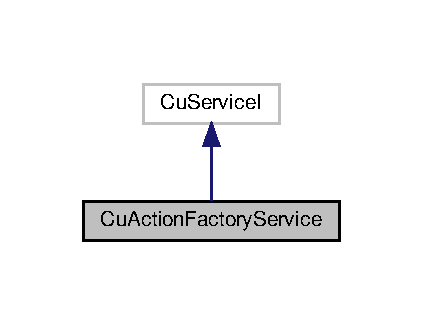
\includegraphics[width=203pt]{classCuActionFactoryService__inherit__graph}
\end{center}
\end{figure}
\subsection*{Public Types}
\begin{DoxyCompactItemize}
\item 
enum \textbf{ Type} \{ \textbf{ Cu\+Action\+Factory\+Service\+Type} = Cu\+Services\+:\+:User + 21
 \}
\end{DoxyCompactItemize}
\subsection*{Public Member Functions}
\begin{DoxyCompactItemize}
\item 
\textbf{ Cu\+Action\+Factory\+Service} ()
\item 
virtual \textbf{ $\sim$\+Cu\+Action\+Factory\+Service} ()
\item 
\textbf{ Cu\+Epics\+ActionI} $\ast$ \textbf{ register\+Action} (const std\+::string \&src, const \textbf{ Cu\+Epics\+Action\+FactoryI} \&f, \textbf{ Cumbia\+Epics} $\ast$ct)
\item 
\textbf{ Cu\+Epics\+ActionI} $\ast$ \textbf{ find\+Action} (const std\+::string \&name, \textbf{ Cu\+Epics\+Action\+I\+::\+Type} at)
\item 
\textbf{ Cu\+Epics\+ActionI} $\ast$ \textbf{ find\+Action} (const std\+::string \&src, \textbf{ Cu\+Epics\+Action\+I\+::\+Type} at, Cu\+Data\+Listener $\ast$l)
\item 
std\+::string \textbf{ get\+Last\+Error} () const
\item 
void \textbf{ unregister\+Action} (const std\+::string \&src, \textbf{ Cu\+Epics\+Action\+I\+::\+Type} at)
\item 
void \textbf{ delete\+Actions} ()
\item 
std\+::string \textbf{ get\+Name} () const
\item 
Cu\+Services\+::\+Type \textbf{ get\+Type} () const
\end{DoxyCompactItemize}


\subsection{Member Enumeration Documentation}
\mbox{\label{classCuActionFactoryService_ad2bb6770622dc3dc24a5846f818e8bdc}} 
\index{Cu\+Action\+Factory\+Service@{Cu\+Action\+Factory\+Service}!Type@{Type}}
\index{Type@{Type}!Cu\+Action\+Factory\+Service@{Cu\+Action\+Factory\+Service}}
\subsubsection{Type}
{\footnotesize\ttfamily enum \textbf{ Cu\+Action\+Factory\+Service\+::\+Type}}

\begin{DoxyEnumFields}{Enumerator}
\raisebox{\heightof{T}}[0pt][0pt]{\index{Cu\+Action\+Factory\+Service\+Type@{Cu\+Action\+Factory\+Service\+Type}!Cu\+Action\+Factory\+Service@{Cu\+Action\+Factory\+Service}}\index{Cu\+Action\+Factory\+Service@{Cu\+Action\+Factory\+Service}!Cu\+Action\+Factory\+Service\+Type@{Cu\+Action\+Factory\+Service\+Type}}}\mbox{\label{classCuActionFactoryService_ad2bb6770622dc3dc24a5846f818e8bdcafb23f61f823444e6df483206eb9b7e11}} 
Cu\+Action\+Factory\+Service\+Type&\\
\hline

\end{DoxyEnumFields}


\subsection{Constructor \& Destructor Documentation}
\mbox{\label{classCuActionFactoryService_a2abdf4c25df1445768d4da7c04df50dd}} 
\index{Cu\+Action\+Factory\+Service@{Cu\+Action\+Factory\+Service}!Cu\+Action\+Factory\+Service@{Cu\+Action\+Factory\+Service}}
\index{Cu\+Action\+Factory\+Service@{Cu\+Action\+Factory\+Service}!Cu\+Action\+Factory\+Service@{Cu\+Action\+Factory\+Service}}
\subsubsection{Cu\+Action\+Factory\+Service()}
{\footnotesize\ttfamily Cu\+Action\+Factory\+Service\+::\+Cu\+Action\+Factory\+Service (\begin{DoxyParamCaption}{ }\end{DoxyParamCaption})}



References Cu\+Action\+Factory\+Service\+Private\+::log, and Cu\+Action\+Factory\+Service\+Private\+::log\+Impl.

\mbox{\label{classCuActionFactoryService_a6555fc4a7ea2d07e1a9cb3080c690a54}} 
\index{Cu\+Action\+Factory\+Service@{Cu\+Action\+Factory\+Service}!````~Cu\+Action\+Factory\+Service@{$\sim$\+Cu\+Action\+Factory\+Service}}
\index{````~Cu\+Action\+Factory\+Service@{$\sim$\+Cu\+Action\+Factory\+Service}!Cu\+Action\+Factory\+Service@{Cu\+Action\+Factory\+Service}}
\subsubsection{$\sim$\+Cu\+Action\+Factory\+Service()}
{\footnotesize\ttfamily Cu\+Action\+Factory\+Service\+::$\sim$\+Cu\+Action\+Factory\+Service (\begin{DoxyParamCaption}{ }\end{DoxyParamCaption})\hspace{0.3cm}{\ttfamily [virtual]}}



References Cu\+Action\+Factory\+Service\+Private\+::log, and Cu\+Action\+Factory\+Service\+Private\+::log\+Impl.



\subsection{Member Function Documentation}
\mbox{\label{classCuActionFactoryService_af343d01dcdd88642a684fb091fd3701e}} 
\index{Cu\+Action\+Factory\+Service@{Cu\+Action\+Factory\+Service}!delete\+Actions@{delete\+Actions}}
\index{delete\+Actions@{delete\+Actions}!Cu\+Action\+Factory\+Service@{Cu\+Action\+Factory\+Service}}
\subsubsection{delete\+Actions()}
{\footnotesize\ttfamily void Cu\+Action\+Factory\+Service\+::delete\+Actions (\begin{DoxyParamCaption}{ }\end{DoxyParamCaption})}



References Cu\+Action\+Factory\+Service\+Private\+::actions, and Cu\+Action\+Factory\+Service\+Private\+::mutex.



Referenced by Cumbia\+Epics\+::$\sim$\+Cumbia\+Epics().

\mbox{\label{classCuActionFactoryService_a91f61fed56b625368e433fd8a27cb6f8}} 
\index{Cu\+Action\+Factory\+Service@{Cu\+Action\+Factory\+Service}!find\+Action@{find\+Action}}
\index{find\+Action@{find\+Action}!Cu\+Action\+Factory\+Service@{Cu\+Action\+Factory\+Service}}
\subsubsection{find\+Action()\hspace{0.1cm}{\footnotesize\ttfamily [1/2]}}
{\footnotesize\ttfamily \textbf{ Cu\+Epics\+ActionI}$\ast$ Cu\+Action\+Factory\+Service\+::find\+Action (\begin{DoxyParamCaption}\item[{const std\+::string \&}]{name,  }\item[{\textbf{ Cu\+Epics\+Action\+I\+::\+Type}}]{at }\end{DoxyParamCaption})}



Referenced by Cumbia\+Epics\+::add\+Action(), Cumbia\+Epics\+::find\+Action(), and Cumbia\+Epics\+::unlink\+Listener().

\mbox{\label{classCuActionFactoryService_a22e2c9c85c25782c0eddda54a5a9c340}} 
\index{Cu\+Action\+Factory\+Service@{Cu\+Action\+Factory\+Service}!find\+Action@{find\+Action}}
\index{find\+Action@{find\+Action}!Cu\+Action\+Factory\+Service@{Cu\+Action\+Factory\+Service}}
\subsubsection{find\+Action()\hspace{0.1cm}{\footnotesize\ttfamily [2/2]}}
{\footnotesize\ttfamily \textbf{ Cu\+Epics\+ActionI} $\ast$ Cu\+Action\+Factory\+Service\+::find\+Action (\begin{DoxyParamCaption}\item[{const std\+::string \&}]{src,  }\item[{\textbf{ Cu\+Epics\+Action\+I\+::\+Type}}]{at,  }\item[{Cu\+Data\+Listener $\ast$}]{l }\end{DoxyParamCaption})}



References Cu\+Action\+Factory\+Service\+Private\+::actions, and Cu\+Action\+Factory\+Service\+Private\+::mutex.

\mbox{\label{classCuActionFactoryService_ad6eda198d36413ff1e5c45f4ec96cc9a}} 
\index{Cu\+Action\+Factory\+Service@{Cu\+Action\+Factory\+Service}!get\+Last\+Error@{get\+Last\+Error}}
\index{get\+Last\+Error@{get\+Last\+Error}!Cu\+Action\+Factory\+Service@{Cu\+Action\+Factory\+Service}}
\subsubsection{get\+Last\+Error()}
{\footnotesize\ttfamily string Cu\+Action\+Factory\+Service\+::get\+Last\+Error (\begin{DoxyParamCaption}{ }\end{DoxyParamCaption}) const}



References Cu\+Action\+Factory\+Service\+Private\+::last\+Error.

\mbox{\label{classCuActionFactoryService_aa13ec3fcb56035e6f8a9137f1b2d3b6a}} 
\index{Cu\+Action\+Factory\+Service@{Cu\+Action\+Factory\+Service}!get\+Name@{get\+Name}}
\index{get\+Name@{get\+Name}!Cu\+Action\+Factory\+Service@{Cu\+Action\+Factory\+Service}}
\subsubsection{get\+Name()}
{\footnotesize\ttfamily std\+::string Cu\+Action\+Factory\+Service\+::get\+Name (\begin{DoxyParamCaption}{ }\end{DoxyParamCaption}) const}

\mbox{\label{classCuActionFactoryService_a1ec587dda23b3cdfdcc7b78b170ed7e3}} 
\index{Cu\+Action\+Factory\+Service@{Cu\+Action\+Factory\+Service}!get\+Type@{get\+Type}}
\index{get\+Type@{get\+Type}!Cu\+Action\+Factory\+Service@{Cu\+Action\+Factory\+Service}}
\subsubsection{get\+Type()}
{\footnotesize\ttfamily Cu\+Services\+::\+Type Cu\+Action\+Factory\+Service\+::get\+Type (\begin{DoxyParamCaption}{ }\end{DoxyParamCaption}) const}



References Cu\+Action\+Factory\+Service\+Type.

\mbox{\label{classCuActionFactoryService_adb063732f244608930bdd1961ddcc33c}} 
\index{Cu\+Action\+Factory\+Service@{Cu\+Action\+Factory\+Service}!register\+Action@{register\+Action}}
\index{register\+Action@{register\+Action}!Cu\+Action\+Factory\+Service@{Cu\+Action\+Factory\+Service}}
\subsubsection{register\+Action()}
{\footnotesize\ttfamily \textbf{ Cu\+Epics\+ActionI} $\ast$ Cu\+Action\+Factory\+Service\+::register\+Action (\begin{DoxyParamCaption}\item[{const std\+::string \&}]{src,  }\item[{const \textbf{ Cu\+Epics\+Action\+FactoryI} \&}]{f,  }\item[{\textbf{ Cumbia\+Epics} $\ast$}]{ct }\end{DoxyParamCaption})}



References Cu\+Action\+Factory\+Service\+Private\+::actions, Cu\+Epics\+Action\+Factory\+I\+::create(), Cu\+Epics\+Action\+Factory\+I\+::get\+Type(), and Cu\+Action\+Factory\+Service\+Private\+::mutex.



Referenced by Cumbia\+Epics\+::add\+Action().

\mbox{\label{classCuActionFactoryService_adc725da0c6a8e068b76aa4daaefb5f45}} 
\index{Cu\+Action\+Factory\+Service@{Cu\+Action\+Factory\+Service}!unregister\+Action@{unregister\+Action}}
\index{unregister\+Action@{unregister\+Action}!Cu\+Action\+Factory\+Service@{Cu\+Action\+Factory\+Service}}
\subsubsection{unregister\+Action()}
{\footnotesize\ttfamily void Cu\+Action\+Factory\+Service\+::unregister\+Action (\begin{DoxyParamCaption}\item[{const std\+::string \&}]{src,  }\item[{\textbf{ Cu\+Epics\+Action\+I\+::\+Type}}]{at }\end{DoxyParamCaption})}



References Cu\+Action\+Factory\+Service\+Private\+::actions, and Cu\+Action\+Factory\+Service\+Private\+::mutex.



Referenced by Cu\+Put\+::on\+Result(), Cu\+Ep\+Configuration\+::on\+Result(), and Cu\+Monitor\+::on\+Result().



The documentation for this class was generated from the following files\+:\begin{DoxyCompactItemize}
\item 
\textbf{ cuepactionfactoryservice.\+h}\item 
\textbf{ cuepactionfactoryservice.\+cpp}\end{DoxyCompactItemize}

\section{Cu\+Action\+Factory\+Service\+Private Class Reference}
\label{classCuActionFactoryServicePrivate}\index{Cu\+Action\+Factory\+Service\+Private@{Cu\+Action\+Factory\+Service\+Private}}
\subsection*{Public Attributes}
\begin{DoxyCompactItemize}
\item 
std\+::list$<$ \textbf{ Cu\+Epics\+ActionI} $\ast$$>$ \textbf{ actions}
\item 
std\+::mutex \textbf{ mutex}
\item 
std\+::string \textbf{ last\+Error}
\item 
Cu\+Log $\ast$ \textbf{ log}
\item 
Cu\+Log\+ImplI $\ast$ \textbf{ log\+Impl}
\end{DoxyCompactItemize}


\subsection{Member Data Documentation}
\mbox{\label{classCuActionFactoryServicePrivate_a502adf0b8a4a3bc68922f5977eb2d179}} 
\index{Cu\+Action\+Factory\+Service\+Private@{Cu\+Action\+Factory\+Service\+Private}!actions@{actions}}
\index{actions@{actions}!Cu\+Action\+Factory\+Service\+Private@{Cu\+Action\+Factory\+Service\+Private}}
\subsubsection{actions}
{\footnotesize\ttfamily std\+::list$<$\textbf{ Cu\+Epics\+ActionI} $\ast$ $>$ Cu\+Action\+Factory\+Service\+Private\+::actions}



Referenced by Cu\+Action\+Factory\+Service\+::delete\+Actions(), Cu\+Action\+Factory\+Service\+::find\+Action(), Cu\+Action\+Factory\+Service\+::register\+Action(), and Cu\+Action\+Factory\+Service\+::unregister\+Action().

\mbox{\label{classCuActionFactoryServicePrivate_a36106c47d6eee3f8bfcccfe8c8e22480}} 
\index{Cu\+Action\+Factory\+Service\+Private@{Cu\+Action\+Factory\+Service\+Private}!last\+Error@{last\+Error}}
\index{last\+Error@{last\+Error}!Cu\+Action\+Factory\+Service\+Private@{Cu\+Action\+Factory\+Service\+Private}}
\subsubsection{last\+Error}
{\footnotesize\ttfamily std\+::string Cu\+Action\+Factory\+Service\+Private\+::last\+Error}



Referenced by Cu\+Action\+Factory\+Service\+::get\+Last\+Error().

\mbox{\label{classCuActionFactoryServicePrivate_a4091f273cc929ea6d1d1593fc8e71801}} 
\index{Cu\+Action\+Factory\+Service\+Private@{Cu\+Action\+Factory\+Service\+Private}!log@{log}}
\index{log@{log}!Cu\+Action\+Factory\+Service\+Private@{Cu\+Action\+Factory\+Service\+Private}}
\subsubsection{log}
{\footnotesize\ttfamily Cu\+Log$\ast$ Cu\+Action\+Factory\+Service\+Private\+::log}



Referenced by Cu\+Action\+Factory\+Service\+::\+Cu\+Action\+Factory\+Service(), and Cu\+Action\+Factory\+Service\+::$\sim$\+Cu\+Action\+Factory\+Service().

\mbox{\label{classCuActionFactoryServicePrivate_aa9d42615edd8d492e5e19fa1a92076a3}} 
\index{Cu\+Action\+Factory\+Service\+Private@{Cu\+Action\+Factory\+Service\+Private}!log\+Impl@{log\+Impl}}
\index{log\+Impl@{log\+Impl}!Cu\+Action\+Factory\+Service\+Private@{Cu\+Action\+Factory\+Service\+Private}}
\subsubsection{log\+Impl}
{\footnotesize\ttfamily Cu\+Log\+ImplI$\ast$ Cu\+Action\+Factory\+Service\+Private\+::log\+Impl}



Referenced by Cu\+Action\+Factory\+Service\+::\+Cu\+Action\+Factory\+Service(), and Cu\+Action\+Factory\+Service\+::$\sim$\+Cu\+Action\+Factory\+Service().

\mbox{\label{classCuActionFactoryServicePrivate_a6035d66853a23e784840834ad06954d3}} 
\index{Cu\+Action\+Factory\+Service\+Private@{Cu\+Action\+Factory\+Service\+Private}!mutex@{mutex}}
\index{mutex@{mutex}!Cu\+Action\+Factory\+Service\+Private@{Cu\+Action\+Factory\+Service\+Private}}
\subsubsection{mutex}
{\footnotesize\ttfamily std\+::mutex Cu\+Action\+Factory\+Service\+Private\+::mutex}



Referenced by Cu\+Action\+Factory\+Service\+::delete\+Actions(), Cu\+Action\+Factory\+Service\+::find\+Action(), Cu\+Action\+Factory\+Service\+::register\+Action(), and Cu\+Action\+Factory\+Service\+::unregister\+Action().



The documentation for this class was generated from the following file\+:\begin{DoxyCompactItemize}
\item 
\textbf{ cuepactionfactoryservice.\+cpp}\end{DoxyCompactItemize}

\section{Cu\+Ep\+C\+A\+Service Class Reference}
\label{classCuEpCAService}\index{Cu\+Ep\+C\+A\+Service@{Cu\+Ep\+C\+A\+Service}}


{\ttfamily \#include $<$cuepcaservice.\+h$>$}



Inheritance diagram for Cu\+Ep\+C\+A\+Service\+:\nopagebreak
\begin{figure}[H]
\begin{center}
\leavevmode
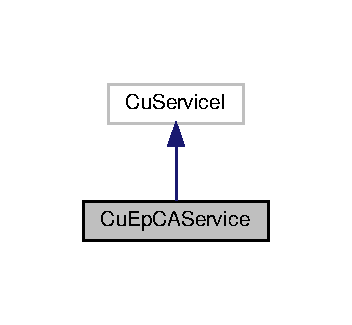
\includegraphics[width=169pt]{classCuEpCAService__inherit__graph}
\end{center}
\end{figure}
\subsection*{Public Types}
\begin{DoxyCompactItemize}
\item 
enum \textbf{ Type} \{ \textbf{ Cu\+Epics\+Channel\+Access\+Service\+Type} = Cu\+Services\+:\+:User + 30
 \}
\end{DoxyCompactItemize}
\subsection*{Public Member Functions}
\begin{DoxyCompactItemize}
\item 
\textbf{ Cu\+Ep\+C\+A\+Service} ()
\item 
virtual \textbf{ $\sim$\+Cu\+Ep\+C\+A\+Service} ()
\item 
int \textbf{ get\+Result} () const
\item 
std\+::string \textbf{ get\+Status} () const
\item 
std\+::\+\_\+\+\_\+cxx11\+::string \textbf{ get\+Name} () const
\item 
Cu\+Services\+::\+Type \textbf{ get\+Type} () const
\end{DoxyCompactItemize}


\subsection{Member Enumeration Documentation}
\mbox{\label{classCuEpCAService_adcdba168d756f3897faa7d3ebe47aaa6}} 
\index{Cu\+Ep\+C\+A\+Service@{Cu\+Ep\+C\+A\+Service}!Type@{Type}}
\index{Type@{Type}!Cu\+Ep\+C\+A\+Service@{Cu\+Ep\+C\+A\+Service}}
\subsubsection{Type}
{\footnotesize\ttfamily enum \textbf{ Cu\+Ep\+C\+A\+Service\+::\+Type}}

\begin{DoxyEnumFields}{Enumerator}
\raisebox{\heightof{T}}[0pt][0pt]{\index{Cu\+Epics\+Channel\+Access\+Service\+Type@{Cu\+Epics\+Channel\+Access\+Service\+Type}!Cu\+Ep\+C\+A\+Service@{Cu\+Ep\+C\+A\+Service}}\index{Cu\+Ep\+C\+A\+Service@{Cu\+Ep\+C\+A\+Service}!Cu\+Epics\+Channel\+Access\+Service\+Type@{Cu\+Epics\+Channel\+Access\+Service\+Type}}}\mbox{\label{classCuEpCAService_adcdba168d756f3897faa7d3ebe47aaa6aea3ba7dcbe8a2a30b8a5c7704055ae7c}} 
Cu\+Epics\+Channel\+Access\+Service\+Type&\\
\hline

\end{DoxyEnumFields}


\subsection{Constructor \& Destructor Documentation}
\mbox{\label{classCuEpCAService_aa06ad84872aa80a6bb25c986ba69a9db}} 
\index{Cu\+Ep\+C\+A\+Service@{Cu\+Ep\+C\+A\+Service}!Cu\+Ep\+C\+A\+Service@{Cu\+Ep\+C\+A\+Service}}
\index{Cu\+Ep\+C\+A\+Service@{Cu\+Ep\+C\+A\+Service}!Cu\+Ep\+C\+A\+Service@{Cu\+Ep\+C\+A\+Service}}
\subsubsection{Cu\+Ep\+C\+A\+Service()}
{\footnotesize\ttfamily Cu\+Ep\+C\+A\+Service\+::\+Cu\+Ep\+C\+A\+Service (\begin{DoxyParamCaption}{ }\end{DoxyParamCaption})}

\mbox{\label{classCuEpCAService_aa8b4a8fd8b45d7ff1583bad25791de49}} 
\index{Cu\+Ep\+C\+A\+Service@{Cu\+Ep\+C\+A\+Service}!````~Cu\+Ep\+C\+A\+Service@{$\sim$\+Cu\+Ep\+C\+A\+Service}}
\index{````~Cu\+Ep\+C\+A\+Service@{$\sim$\+Cu\+Ep\+C\+A\+Service}!Cu\+Ep\+C\+A\+Service@{Cu\+Ep\+C\+A\+Service}}
\subsubsection{$\sim$\+Cu\+Ep\+C\+A\+Service()}
{\footnotesize\ttfamily Cu\+Ep\+C\+A\+Service\+::$\sim$\+Cu\+Ep\+C\+A\+Service (\begin{DoxyParamCaption}{ }\end{DoxyParamCaption})\hspace{0.3cm}{\ttfamily [virtual]}}



\subsection{Member Function Documentation}
\mbox{\label{classCuEpCAService_abd0d2b61db9f51c134f95202f29fd458}} 
\index{Cu\+Ep\+C\+A\+Service@{Cu\+Ep\+C\+A\+Service}!get\+Name@{get\+Name}}
\index{get\+Name@{get\+Name}!Cu\+Ep\+C\+A\+Service@{Cu\+Ep\+C\+A\+Service}}
\subsubsection{get\+Name()}
{\footnotesize\ttfamily std\+::\+\_\+\+\_\+cxx11\+::string Cu\+Ep\+C\+A\+Service\+::get\+Name (\begin{DoxyParamCaption}{ }\end{DoxyParamCaption}) const}

\mbox{\label{classCuEpCAService_aeb8902066b2106726400024072a5b926}} 
\index{Cu\+Ep\+C\+A\+Service@{Cu\+Ep\+C\+A\+Service}!get\+Result@{get\+Result}}
\index{get\+Result@{get\+Result}!Cu\+Ep\+C\+A\+Service@{Cu\+Ep\+C\+A\+Service}}
\subsubsection{get\+Result()}
{\footnotesize\ttfamily int Cu\+Ep\+C\+A\+Service\+::get\+Result (\begin{DoxyParamCaption}{ }\end{DoxyParamCaption}) const}

\mbox{\label{classCuEpCAService_a16a550d2dd24d730fd424bce8a6210d4}} 
\index{Cu\+Ep\+C\+A\+Service@{Cu\+Ep\+C\+A\+Service}!get\+Status@{get\+Status}}
\index{get\+Status@{get\+Status}!Cu\+Ep\+C\+A\+Service@{Cu\+Ep\+C\+A\+Service}}
\subsubsection{get\+Status()}
{\footnotesize\ttfamily string Cu\+Ep\+C\+A\+Service\+::get\+Status (\begin{DoxyParamCaption}{ }\end{DoxyParamCaption}) const}

\mbox{\label{classCuEpCAService_a6ad34e2bf4b442b315cded512d611cf3}} 
\index{Cu\+Ep\+C\+A\+Service@{Cu\+Ep\+C\+A\+Service}!get\+Type@{get\+Type}}
\index{get\+Type@{get\+Type}!Cu\+Ep\+C\+A\+Service@{Cu\+Ep\+C\+A\+Service}}
\subsubsection{get\+Type()}
{\footnotesize\ttfamily Cu\+Services\+::\+Type Cu\+Ep\+C\+A\+Service\+::get\+Type (\begin{DoxyParamCaption}{ }\end{DoxyParamCaption}) const}



References Cu\+Epics\+Channel\+Access\+Service\+Type.



The documentation for this class was generated from the following files\+:\begin{DoxyCompactItemize}
\item 
\textbf{ cuepcaservice.\+h}\item 
\textbf{ cuepcaservice.\+cpp}\end{DoxyCompactItemize}

\section{Cu\+Ep\+Config\+Activity Class Reference}
\label{classCuEpConfigActivity}\index{Cu\+Ep\+Config\+Activity@{Cu\+Ep\+Config\+Activity}}


{\ttfamily \#include $<$cuepconfigactivity.\+h$>$}



Inheritance diagram for Cu\+Ep\+Config\+Activity\+:\nopagebreak
\begin{figure}[H]
\begin{center}
\leavevmode
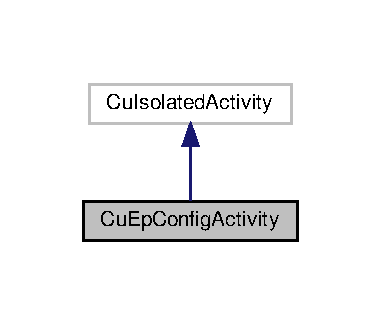
\includegraphics[width=183pt]{classCuEpConfigActivity__inherit__graph}
\end{center}
\end{figure}
\subsection*{Public Types}
\begin{DoxyCompactItemize}
\item 
enum \textbf{ Type} \{ \textbf{ Cu\+Att\+Config\+Activity\+Type} = Cu\+Activity\+:\+:User + 5
 \}
\end{DoxyCompactItemize}
\subsection*{Public Member Functions}
\begin{DoxyCompactItemize}
\item 
\textbf{ Cu\+Ep\+Config\+Activity} (const Cu\+Data \&tok, \textbf{ Cu\+Ep\+C\+A\+Service} $\ast$df)
\item 
void \textbf{ set\+Desired\+Attribute\+Properties} (const std\+::vector$<$ std\+::string $>$ \&props)
\item 
virtual \textbf{ $\sim$\+Cu\+Ep\+Config\+Activity} ()
\item 
int \textbf{ get\+Type} () const
\item 
void \textbf{ event} (Cu\+Activity\+Event $\ast$e)
\item 
bool \textbf{ matches} (const Cu\+Data \&token) const
\item 
int \textbf{ repeat} () const
\end{DoxyCompactItemize}
\subsection*{Protected Member Functions}
\begin{DoxyCompactItemize}
\item 
void \textbf{ init} ()
\item 
void \textbf{ execute} ()
\item 
void \textbf{ on\+Exit} ()
\end{DoxyCompactItemize}


\subsection{Member Enumeration Documentation}
\mbox{\label{classCuEpConfigActivity_ad97b7e37d22827c7f502c536d0a7839b}} 
\index{Cu\+Ep\+Config\+Activity@{Cu\+Ep\+Config\+Activity}!Type@{Type}}
\index{Type@{Type}!Cu\+Ep\+Config\+Activity@{Cu\+Ep\+Config\+Activity}}
\subsubsection{Type}
{\footnotesize\ttfamily enum \textbf{ Cu\+Ep\+Config\+Activity\+::\+Type}}

\begin{DoxyEnumFields}{Enumerator}
\raisebox{\heightof{T}}[0pt][0pt]{\index{Cu\+Att\+Config\+Activity\+Type@{Cu\+Att\+Config\+Activity\+Type}!Cu\+Ep\+Config\+Activity@{Cu\+Ep\+Config\+Activity}}\index{Cu\+Ep\+Config\+Activity@{Cu\+Ep\+Config\+Activity}!Cu\+Att\+Config\+Activity\+Type@{Cu\+Att\+Config\+Activity\+Type}}}\mbox{\label{classCuEpConfigActivity_ad97b7e37d22827c7f502c536d0a7839ba43fc0fe99f1fcfe4bf31e8f05acfce04}} 
Cu\+Att\+Config\+Activity\+Type&\\
\hline

\end{DoxyEnumFields}


\subsection{Constructor \& Destructor Documentation}
\mbox{\label{classCuEpConfigActivity_a246067a4a8d5ea1a71e34c76fe149f6b}} 
\index{Cu\+Ep\+Config\+Activity@{Cu\+Ep\+Config\+Activity}!Cu\+Ep\+Config\+Activity@{Cu\+Ep\+Config\+Activity}}
\index{Cu\+Ep\+Config\+Activity@{Cu\+Ep\+Config\+Activity}!Cu\+Ep\+Config\+Activity@{Cu\+Ep\+Config\+Activity}}
\subsubsection{Cu\+Ep\+Config\+Activity()}
{\footnotesize\ttfamily Cu\+Ep\+Config\+Activity\+::\+Cu\+Ep\+Config\+Activity (\begin{DoxyParamCaption}\item[{const Cu\+Data \&}]{tok,  }\item[{\textbf{ Cu\+Ep\+C\+A\+Service} $\ast$}]{df }\end{DoxyParamCaption})}



References Cu\+Ep\+Config\+Activity\+Private\+::ep\+\_\+service, Cu\+Ep\+Config\+Activity\+Private\+::err, Cu\+Ep\+Config\+Activity\+Private\+::exiting, and Cu\+Ep\+Config\+Activity\+Private\+::other\+\_\+thread\+\_\+id.

\mbox{\label{classCuEpConfigActivity_ae9597a3d808a75787032e3281eb9a726}} 
\index{Cu\+Ep\+Config\+Activity@{Cu\+Ep\+Config\+Activity}!````~Cu\+Ep\+Config\+Activity@{$\sim$\+Cu\+Ep\+Config\+Activity}}
\index{````~Cu\+Ep\+Config\+Activity@{$\sim$\+Cu\+Ep\+Config\+Activity}!Cu\+Ep\+Config\+Activity@{Cu\+Ep\+Config\+Activity}}
\subsubsection{$\sim$\+Cu\+Ep\+Config\+Activity()}
{\footnotesize\ttfamily Cu\+Ep\+Config\+Activity\+::$\sim$\+Cu\+Ep\+Config\+Activity (\begin{DoxyParamCaption}{ }\end{DoxyParamCaption})\hspace{0.3cm}{\ttfamily [virtual]}}



\subsection{Member Function Documentation}
\mbox{\label{classCuEpConfigActivity_af9199f7b7db2d37c23a513176bae0421}} 
\index{Cu\+Ep\+Config\+Activity@{Cu\+Ep\+Config\+Activity}!event@{event}}
\index{event@{event}!Cu\+Ep\+Config\+Activity@{Cu\+Ep\+Config\+Activity}}
\subsubsection{event()}
{\footnotesize\ttfamily void Cu\+Ep\+Config\+Activity\+::event (\begin{DoxyParamCaption}\item[{Cu\+Activity\+Event $\ast$}]{e }\end{DoxyParamCaption})}

\mbox{\label{classCuEpConfigActivity_a708ea3f341b7fc34110015fedbfdab59}} 
\index{Cu\+Ep\+Config\+Activity@{Cu\+Ep\+Config\+Activity}!execute@{execute}}
\index{execute@{execute}!Cu\+Ep\+Config\+Activity@{Cu\+Ep\+Config\+Activity}}
\subsubsection{execute()}
{\footnotesize\ttfamily void Cu\+Ep\+Config\+Activity\+::execute (\begin{DoxyParamCaption}{ }\end{DoxyParamCaption})\hspace{0.3cm}{\ttfamily [protected]}}



References Cu\+Ep\+Config\+Activity\+Private\+::err, Cu\+Epics\+World\+::fill\+Thread\+Info(), Cu\+Ep\+Config\+Activity\+Private\+::msg, and Cu\+Ep\+Config\+Activity\+Private\+::my\+\_\+thread\+\_\+id.

\mbox{\label{classCuEpConfigActivity_ae92b93cb2a17303daf9eb7d4702c43b8}} 
\index{Cu\+Ep\+Config\+Activity@{Cu\+Ep\+Config\+Activity}!get\+Type@{get\+Type}}
\index{get\+Type@{get\+Type}!Cu\+Ep\+Config\+Activity@{Cu\+Ep\+Config\+Activity}}
\subsubsection{get\+Type()}
{\footnotesize\ttfamily int Cu\+Ep\+Config\+Activity\+::get\+Type (\begin{DoxyParamCaption}{ }\end{DoxyParamCaption}) const}



References Cu\+Att\+Config\+Activity\+Type.

\mbox{\label{classCuEpConfigActivity_a2ce6d85ed44cb4bafaca0ea1341a50a8}} 
\index{Cu\+Ep\+Config\+Activity@{Cu\+Ep\+Config\+Activity}!init@{init}}
\index{init@{init}!Cu\+Ep\+Config\+Activity@{Cu\+Ep\+Config\+Activity}}
\subsubsection{init()}
{\footnotesize\ttfamily void Cu\+Ep\+Config\+Activity\+::init (\begin{DoxyParamCaption}{ }\end{DoxyParamCaption})\hspace{0.3cm}{\ttfamily [protected]}}



References Cu\+Ep\+Config\+Activity\+Private\+::my\+\_\+thread\+\_\+id, and Cu\+Ep\+Config\+Activity\+Private\+::other\+\_\+thread\+\_\+id.

\mbox{\label{classCuEpConfigActivity_aeba28440d3334d01a17c2968f1dd8271}} 
\index{Cu\+Ep\+Config\+Activity@{Cu\+Ep\+Config\+Activity}!matches@{matches}}
\index{matches@{matches}!Cu\+Ep\+Config\+Activity@{Cu\+Ep\+Config\+Activity}}
\subsubsection{matches()}
{\footnotesize\ttfamily bool Cu\+Ep\+Config\+Activity\+::matches (\begin{DoxyParamCaption}\item[{const Cu\+Data \&}]{token }\end{DoxyParamCaption}) const}

\mbox{\label{classCuEpConfigActivity_af9037bd055fdb74ee7ab29e37306b814}} 
\index{Cu\+Ep\+Config\+Activity@{Cu\+Ep\+Config\+Activity}!on\+Exit@{on\+Exit}}
\index{on\+Exit@{on\+Exit}!Cu\+Ep\+Config\+Activity@{Cu\+Ep\+Config\+Activity}}
\subsubsection{on\+Exit()}
{\footnotesize\ttfamily void Cu\+Ep\+Config\+Activity\+::on\+Exit (\begin{DoxyParamCaption}{ }\end{DoxyParamCaption})\hspace{0.3cm}{\ttfamily [protected]}}



References Cu\+Ep\+Config\+Activity\+Private\+::err, Cu\+Ep\+Config\+Activity\+Private\+::exiting, Cu\+Epics\+World\+::fill\+Thread\+Info(), Cu\+Ep\+Config\+Activity\+Private\+::msg, and Cu\+Ep\+Config\+Activity\+Private\+::my\+\_\+thread\+\_\+id.

\mbox{\label{classCuEpConfigActivity_afca293c4f124ca27f464f210b11b8ed4}} 
\index{Cu\+Ep\+Config\+Activity@{Cu\+Ep\+Config\+Activity}!repeat@{repeat}}
\index{repeat@{repeat}!Cu\+Ep\+Config\+Activity@{Cu\+Ep\+Config\+Activity}}
\subsubsection{repeat()}
{\footnotesize\ttfamily int Cu\+Ep\+Config\+Activity\+::repeat (\begin{DoxyParamCaption}{ }\end{DoxyParamCaption}) const}

\mbox{\label{classCuEpConfigActivity_aba4a5e72e609367f58b975a5df9f91c2}} 
\index{Cu\+Ep\+Config\+Activity@{Cu\+Ep\+Config\+Activity}!set\+Desired\+Attribute\+Properties@{set\+Desired\+Attribute\+Properties}}
\index{set\+Desired\+Attribute\+Properties@{set\+Desired\+Attribute\+Properties}!Cu\+Ep\+Config\+Activity@{Cu\+Ep\+Config\+Activity}}
\subsubsection{set\+Desired\+Attribute\+Properties()}
{\footnotesize\ttfamily void Cu\+Ep\+Config\+Activity\+::set\+Desired\+Attribute\+Properties (\begin{DoxyParamCaption}\item[{const std\+::vector$<$ std\+::string $>$ \&}]{props }\end{DoxyParamCaption})}



References Cu\+Ep\+Config\+Activity\+Private\+::props.



The documentation for this class was generated from the following files\+:\begin{DoxyCompactItemize}
\item 
\textbf{ cuepconfigactivity.\+h}\item 
\textbf{ cuepconfigactivity.\+cpp}\end{DoxyCompactItemize}

\section{Cu\+Ep\+Config\+Activity\+Private Class Reference}
\label{classCuEpConfigActivityPrivate}\index{Cu\+Ep\+Config\+Activity\+Private@{Cu\+Ep\+Config\+Activity\+Private}}
\subsection*{Public Attributes}
\begin{DoxyCompactItemize}
\item 
\textbf{ Cu\+Ep\+C\+A\+Service} $\ast$ \textbf{ ep\+\_\+service}
\item 
std\+::string \textbf{ msg}
\item 
bool \textbf{ err}
\item 
pthread\+\_\+t \textbf{ my\+\_\+thread\+\_\+id}
\item 
pthread\+\_\+t \textbf{ other\+\_\+thread\+\_\+id}
\item 
std\+::vector$<$ std\+::string $>$ \textbf{ props}
\item 
bool \textbf{ exiting}
\end{DoxyCompactItemize}


\subsection{Member Data Documentation}
\mbox{\label{classCuEpConfigActivityPrivate_a04bb0b3ccf954c6664bab6469545017d}} 
\index{Cu\+Ep\+Config\+Activity\+Private@{Cu\+Ep\+Config\+Activity\+Private}!ep\+\_\+service@{ep\+\_\+service}}
\index{ep\+\_\+service@{ep\+\_\+service}!Cu\+Ep\+Config\+Activity\+Private@{Cu\+Ep\+Config\+Activity\+Private}}
\subsubsection{ep\+\_\+service}
{\footnotesize\ttfamily \textbf{ Cu\+Ep\+C\+A\+Service}$\ast$ Cu\+Ep\+Config\+Activity\+Private\+::ep\+\_\+service}



Referenced by Cu\+Ep\+Config\+Activity\+::\+Cu\+Ep\+Config\+Activity().

\mbox{\label{classCuEpConfigActivityPrivate_ab85123ed5399f3459ddcc6acf9563588}} 
\index{Cu\+Ep\+Config\+Activity\+Private@{Cu\+Ep\+Config\+Activity\+Private}!err@{err}}
\index{err@{err}!Cu\+Ep\+Config\+Activity\+Private@{Cu\+Ep\+Config\+Activity\+Private}}
\subsubsection{err}
{\footnotesize\ttfamily bool Cu\+Ep\+Config\+Activity\+Private\+::err}



Referenced by Cu\+Ep\+Config\+Activity\+::\+Cu\+Ep\+Config\+Activity(), Cu\+Ep\+Config\+Activity\+::execute(), and Cu\+Ep\+Config\+Activity\+::on\+Exit().

\mbox{\label{classCuEpConfigActivityPrivate_a7af8e2037c937736127bc9831356d975}} 
\index{Cu\+Ep\+Config\+Activity\+Private@{Cu\+Ep\+Config\+Activity\+Private}!exiting@{exiting}}
\index{exiting@{exiting}!Cu\+Ep\+Config\+Activity\+Private@{Cu\+Ep\+Config\+Activity\+Private}}
\subsubsection{exiting}
{\footnotesize\ttfamily bool Cu\+Ep\+Config\+Activity\+Private\+::exiting}



Referenced by Cu\+Ep\+Config\+Activity\+::\+Cu\+Ep\+Config\+Activity(), and Cu\+Ep\+Config\+Activity\+::on\+Exit().

\mbox{\label{classCuEpConfigActivityPrivate_a3ce255a920ffc468409c8615d6648bb5}} 
\index{Cu\+Ep\+Config\+Activity\+Private@{Cu\+Ep\+Config\+Activity\+Private}!msg@{msg}}
\index{msg@{msg}!Cu\+Ep\+Config\+Activity\+Private@{Cu\+Ep\+Config\+Activity\+Private}}
\subsubsection{msg}
{\footnotesize\ttfamily std\+::string Cu\+Ep\+Config\+Activity\+Private\+::msg}



Referenced by Cu\+Ep\+Config\+Activity\+::execute(), and Cu\+Ep\+Config\+Activity\+::on\+Exit().

\mbox{\label{classCuEpConfigActivityPrivate_a8ba2277d7f0ccb129ed4a9d87a79e57c}} 
\index{Cu\+Ep\+Config\+Activity\+Private@{Cu\+Ep\+Config\+Activity\+Private}!my\+\_\+thread\+\_\+id@{my\+\_\+thread\+\_\+id}}
\index{my\+\_\+thread\+\_\+id@{my\+\_\+thread\+\_\+id}!Cu\+Ep\+Config\+Activity\+Private@{Cu\+Ep\+Config\+Activity\+Private}}
\subsubsection{my\+\_\+thread\+\_\+id}
{\footnotesize\ttfamily pthread\+\_\+t Cu\+Ep\+Config\+Activity\+Private\+::my\+\_\+thread\+\_\+id}



Referenced by Cu\+Ep\+Config\+Activity\+::execute(), Cu\+Ep\+Config\+Activity\+::init(), and Cu\+Ep\+Config\+Activity\+::on\+Exit().

\mbox{\label{classCuEpConfigActivityPrivate_ade98f30dbb876ad9a87c7c9893f4eb31}} 
\index{Cu\+Ep\+Config\+Activity\+Private@{Cu\+Ep\+Config\+Activity\+Private}!other\+\_\+thread\+\_\+id@{other\+\_\+thread\+\_\+id}}
\index{other\+\_\+thread\+\_\+id@{other\+\_\+thread\+\_\+id}!Cu\+Ep\+Config\+Activity\+Private@{Cu\+Ep\+Config\+Activity\+Private}}
\subsubsection{other\+\_\+thread\+\_\+id}
{\footnotesize\ttfamily pthread\+\_\+t Cu\+Ep\+Config\+Activity\+Private\+::other\+\_\+thread\+\_\+id}



Referenced by Cu\+Ep\+Config\+Activity\+::\+Cu\+Ep\+Config\+Activity(), and Cu\+Ep\+Config\+Activity\+::init().

\mbox{\label{classCuEpConfigActivityPrivate_a71e5bb7d57024f473457208bd13436f5}} 
\index{Cu\+Ep\+Config\+Activity\+Private@{Cu\+Ep\+Config\+Activity\+Private}!props@{props}}
\index{props@{props}!Cu\+Ep\+Config\+Activity\+Private@{Cu\+Ep\+Config\+Activity\+Private}}
\subsubsection{props}
{\footnotesize\ttfamily std\+::vector$<$std\+::string$>$ Cu\+Ep\+Config\+Activity\+Private\+::props}



Referenced by Cu\+Ep\+Config\+Activity\+::set\+Desired\+Attribute\+Properties().



The documentation for this class was generated from the following file\+:\begin{DoxyCompactItemize}
\item 
\textbf{ cuepconfigactivity.\+cpp}\end{DoxyCompactItemize}

\section{Cu\+Ep\+Configuration Class Reference}
\label{classCuEpConfiguration}\index{Cu\+Ep\+Configuration@{Cu\+Ep\+Configuration}}


{\ttfamily \#include $<$cuepconfiguration.\+h$>$}



Inheritance diagram for Cu\+Ep\+Configuration\+:\nopagebreak
\begin{figure}[H]
\begin{center}
\leavevmode
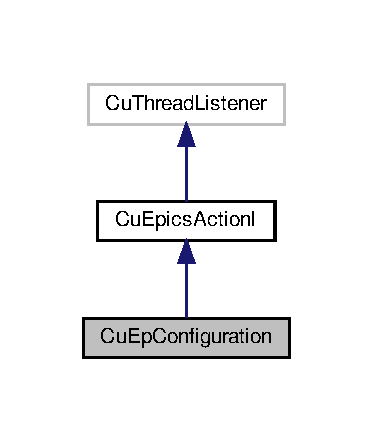
\includegraphics[width=179pt]{classCuEpConfiguration__inherit__graph}
\end{center}
\end{figure}
\subsection*{Public Member Functions}
\begin{DoxyCompactItemize}
\item 
\textbf{ Cu\+Ep\+Configuration} (const \textbf{ Ep\+Source} \&src, \textbf{ Cumbia\+Epics} $\ast$ct)
\item 
virtual \textbf{ $\sim$\+Cu\+Ep\+Configuration} ()
\item 
void \textbf{ set\+Desired\+Attribute\+Properties} (const std\+::vector$<$ std\+::string $>$ props)
\item 
void \textbf{ on\+Progress} (int, int, const Cu\+Data \&)
\item 
void \textbf{ on\+Result} (const Cu\+Data \&data)
\item 
Cu\+Data \textbf{ get\+Token} () const
\item 
\textbf{ Ep\+Source} \textbf{ get\+Source} () const
\item 
\textbf{ Type} \textbf{ get\+Type} () const
\item 
void \textbf{ add\+Data\+Listener} (Cu\+Data\+Listener $\ast$l)
\item 
void \textbf{ remove\+Data\+Listener} (Cu\+Data\+Listener $\ast$l)
\item 
void \textbf{ send\+Data} (const Cu\+Data \&data)
\item 
void \textbf{ get\+Data} (Cu\+Data \&d\+\_\+inout) const
\item 
size\+\_\+t \textbf{ data\+Listeners\+Count} ()
\item 
void \textbf{ start} ()
\item 
void \textbf{ stop} ()
\end{DoxyCompactItemize}
\subsection*{Additional Inherited Members}


\subsection{Constructor \& Destructor Documentation}
\mbox{\label{classCuEpConfiguration_ab7b8c24a042b2c933c6d68bcc0e2665f}} 
\index{Cu\+Ep\+Configuration@{Cu\+Ep\+Configuration}!Cu\+Ep\+Configuration@{Cu\+Ep\+Configuration}}
\index{Cu\+Ep\+Configuration@{Cu\+Ep\+Configuration}!Cu\+Ep\+Configuration@{Cu\+Ep\+Configuration}}
\subsubsection{Cu\+Ep\+Configuration()}
{\footnotesize\ttfamily Cu\+Ep\+Configuration\+::\+Cu\+Ep\+Configuration (\begin{DoxyParamCaption}\item[{const \textbf{ Ep\+Source} \&}]{src,  }\item[{\textbf{ Cumbia\+Epics} $\ast$}]{ct }\end{DoxyParamCaption})}



References Cu\+T\+Att\+Configuration\+Private\+::cumbia\+\_\+t, and Cu\+T\+Att\+Configuration\+Private\+::tsrc.

\mbox{\label{classCuEpConfiguration_a334369fe721dc889042f178ab13ace21}} 
\index{Cu\+Ep\+Configuration@{Cu\+Ep\+Configuration}!````~Cu\+Ep\+Configuration@{$\sim$\+Cu\+Ep\+Configuration}}
\index{````~Cu\+Ep\+Configuration@{$\sim$\+Cu\+Ep\+Configuration}!Cu\+Ep\+Configuration@{Cu\+Ep\+Configuration}}
\subsubsection{$\sim$\+Cu\+Ep\+Configuration()}
{\footnotesize\ttfamily Cu\+Ep\+Configuration\+::$\sim$\+Cu\+Ep\+Configuration (\begin{DoxyParamCaption}{ }\end{DoxyParamCaption})\hspace{0.3cm}{\ttfamily [virtual]}}



\subsection{Member Function Documentation}
\mbox{\label{classCuEpConfiguration_a4f89b2a4514f6d8135d7c2e0c0b626dd}} 
\index{Cu\+Ep\+Configuration@{Cu\+Ep\+Configuration}!add\+Data\+Listener@{add\+Data\+Listener}}
\index{add\+Data\+Listener@{add\+Data\+Listener}!Cu\+Ep\+Configuration@{Cu\+Ep\+Configuration}}
\subsubsection{add\+Data\+Listener()}
{\footnotesize\ttfamily void Cu\+Ep\+Configuration\+::add\+Data\+Listener (\begin{DoxyParamCaption}\item[{Cu\+Data\+Listener $\ast$}]{l }\end{DoxyParamCaption})\hspace{0.3cm}{\ttfamily [virtual]}}



Implements \textbf{ Cu\+Epics\+ActionI} \doxyref{}{p.}{classCuEpicsActionI_a8e6c0261f02cb237d612e097fee6dc4a}.



References Cu\+T\+Att\+Configuration\+Private\+::conf\+\_\+data, and Cu\+T\+Att\+Configuration\+Private\+::listeners.

\mbox{\label{classCuEpConfiguration_ad7c394d3a0b0881091cb7c918b7fd1cf}} 
\index{Cu\+Ep\+Configuration@{Cu\+Ep\+Configuration}!data\+Listeners\+Count@{data\+Listeners\+Count}}
\index{data\+Listeners\+Count@{data\+Listeners\+Count}!Cu\+Ep\+Configuration@{Cu\+Ep\+Configuration}}
\subsubsection{data\+Listeners\+Count()}
{\footnotesize\ttfamily size\+\_\+t Cu\+Ep\+Configuration\+::data\+Listeners\+Count (\begin{DoxyParamCaption}{ }\end{DoxyParamCaption})\hspace{0.3cm}{\ttfamily [virtual]}}



Implements \textbf{ Cu\+Epics\+ActionI} \doxyref{}{p.}{classCuEpicsActionI_af7b509410aaee059c3105dfb10b33ee7}.



References Cu\+T\+Att\+Configuration\+Private\+::listeners.

\mbox{\label{classCuEpConfiguration_a1941fa5e0812068058b17cf9f9827c4d}} 
\index{Cu\+Ep\+Configuration@{Cu\+Ep\+Configuration}!get\+Data@{get\+Data}}
\index{get\+Data@{get\+Data}!Cu\+Ep\+Configuration@{Cu\+Ep\+Configuration}}
\subsubsection{get\+Data()}
{\footnotesize\ttfamily void Cu\+Ep\+Configuration\+::get\+Data (\begin{DoxyParamCaption}\item[{Cu\+Data \&}]{d\+\_\+inout }\end{DoxyParamCaption}) const\hspace{0.3cm}{\ttfamily [virtual]}}



Implements \textbf{ Cu\+Epics\+ActionI} \doxyref{}{p.}{classCuEpicsActionI_a063d9436f8a6b84a22a384d06c3996bd}.

\mbox{\label{classCuEpConfiguration_a3fdc803bd3890ec9a39486ae5e7382b3}} 
\index{Cu\+Ep\+Configuration@{Cu\+Ep\+Configuration}!get\+Source@{get\+Source}}
\index{get\+Source@{get\+Source}!Cu\+Ep\+Configuration@{Cu\+Ep\+Configuration}}
\subsubsection{get\+Source()}
{\footnotesize\ttfamily \textbf{ Ep\+Source} Cu\+Ep\+Configuration\+::get\+Source (\begin{DoxyParamCaption}{ }\end{DoxyParamCaption}) const\hspace{0.3cm}{\ttfamily [virtual]}}



Implements \textbf{ Cu\+Epics\+ActionI} \doxyref{}{p.}{classCuEpicsActionI_a2c97ba6d9bbd9e98fec51aa92d2becb6}.



References Cu\+T\+Att\+Configuration\+Private\+::tsrc.

\mbox{\label{classCuEpConfiguration_a7d87941432e0fdeb549085078808f18c}} 
\index{Cu\+Ep\+Configuration@{Cu\+Ep\+Configuration}!get\+Token@{get\+Token}}
\index{get\+Token@{get\+Token}!Cu\+Ep\+Configuration@{Cu\+Ep\+Configuration}}
\subsubsection{get\+Token()}
{\footnotesize\ttfamily Cu\+Data Cu\+Ep\+Configuration\+::get\+Token (\begin{DoxyParamCaption}{ }\end{DoxyParamCaption}) const}



References Ep\+Source\+::get\+Name(), and Cu\+T\+Att\+Configuration\+Private\+::tsrc.

\mbox{\label{classCuEpConfiguration_afe9b397877ed5311df2176244ca5112f}} 
\index{Cu\+Ep\+Configuration@{Cu\+Ep\+Configuration}!get\+Type@{get\+Type}}
\index{get\+Type@{get\+Type}!Cu\+Ep\+Configuration@{Cu\+Ep\+Configuration}}
\subsubsection{get\+Type()}
{\footnotesize\ttfamily \textbf{ Cu\+Epics\+Action\+I\+::\+Type} Cu\+Ep\+Configuration\+::get\+Type (\begin{DoxyParamCaption}{ }\end{DoxyParamCaption}) const\hspace{0.3cm}{\ttfamily [virtual]}}



Implements \textbf{ Cu\+Epics\+ActionI} \doxyref{}{p.}{classCuEpicsActionI_a7386456fda8f1fe44dac1960842b96a6}.



References Cu\+Epics\+Action\+I\+::\+Att\+Config.



Referenced by on\+Result().

\mbox{\label{classCuEpConfiguration_af05f41610f4f53da34e875124e47ce9b}} 
\index{Cu\+Ep\+Configuration@{Cu\+Ep\+Configuration}!on\+Progress@{on\+Progress}}
\index{on\+Progress@{on\+Progress}!Cu\+Ep\+Configuration@{Cu\+Ep\+Configuration}}
\subsubsection{on\+Progress()}
{\footnotesize\ttfamily void Cu\+Ep\+Configuration\+::on\+Progress (\begin{DoxyParamCaption}\item[{int}]{step,  }\item[{int}]{total,  }\item[{const Cu\+Data \&}]{data }\end{DoxyParamCaption})}

\mbox{\label{classCuEpConfiguration_a8da11e3c75597a821f96d623b4a52e7c}} 
\index{Cu\+Ep\+Configuration@{Cu\+Ep\+Configuration}!on\+Result@{on\+Result}}
\index{on\+Result@{on\+Result}!Cu\+Ep\+Configuration@{Cu\+Ep\+Configuration}}
\subsubsection{on\+Result()}
{\footnotesize\ttfamily void Cu\+Ep\+Configuration\+::on\+Result (\begin{DoxyParamCaption}\item[{const Cu\+Data \&}]{data }\end{DoxyParamCaption})}



References Cu\+T\+Att\+Configuration\+Private\+::conf\+\_\+data, Cu\+Action\+Factory\+Service\+::\+Cu\+Action\+Factory\+Service\+Type, Cu\+T\+Att\+Configuration\+Private\+::cumbia\+\_\+t, Ep\+Source\+::get\+Name(), get\+Type(), Cu\+T\+Att\+Configuration\+Private\+::listeners, Cu\+T\+Att\+Configuration\+Private\+::tsrc, and Cu\+Action\+Factory\+Service\+::unregister\+Action().

\mbox{\label{classCuEpConfiguration_a45ceb248426de776e465bf06ce94e042}} 
\index{Cu\+Ep\+Configuration@{Cu\+Ep\+Configuration}!remove\+Data\+Listener@{remove\+Data\+Listener}}
\index{remove\+Data\+Listener@{remove\+Data\+Listener}!Cu\+Ep\+Configuration@{Cu\+Ep\+Configuration}}
\subsubsection{remove\+Data\+Listener()}
{\footnotesize\ttfamily void Cu\+Ep\+Configuration\+::remove\+Data\+Listener (\begin{DoxyParamCaption}\item[{Cu\+Data\+Listener $\ast$}]{l }\end{DoxyParamCaption})\hspace{0.3cm}{\ttfamily [virtual]}}



Implements \textbf{ Cu\+Epics\+ActionI} \doxyref{}{p.}{classCuEpicsActionI_a5f5c5045ae8f93ed95794538c495dfdf}.



References Cu\+T\+Att\+Configuration\+Private\+::listeners, and stop().

\mbox{\label{classCuEpConfiguration_ad40463466a0d3f298c2bc155115ffcd8}} 
\index{Cu\+Ep\+Configuration@{Cu\+Ep\+Configuration}!send\+Data@{send\+Data}}
\index{send\+Data@{send\+Data}!Cu\+Ep\+Configuration@{Cu\+Ep\+Configuration}}
\subsubsection{send\+Data()}
{\footnotesize\ttfamily void Cu\+Ep\+Configuration\+::send\+Data (\begin{DoxyParamCaption}\item[{const Cu\+Data \&}]{data }\end{DoxyParamCaption})\hspace{0.3cm}{\ttfamily [virtual]}}



Implements \textbf{ Cu\+Epics\+ActionI} \doxyref{}{p.}{classCuEpicsActionI_acced5eb52ec2b30b2f21ca30b043d683}.

\mbox{\label{classCuEpConfiguration_a366242060e397fcab676a1863f87a6d4}} 
\index{Cu\+Ep\+Configuration@{Cu\+Ep\+Configuration}!set\+Desired\+Attribute\+Properties@{set\+Desired\+Attribute\+Properties}}
\index{set\+Desired\+Attribute\+Properties@{set\+Desired\+Attribute\+Properties}!Cu\+Ep\+Configuration@{Cu\+Ep\+Configuration}}
\subsubsection{set\+Desired\+Attribute\+Properties()}
{\footnotesize\ttfamily void Cu\+Ep\+Configuration\+::set\+Desired\+Attribute\+Properties (\begin{DoxyParamCaption}\item[{const std\+::vector$<$ std\+::string $>$}]{props }\end{DoxyParamCaption})}



References Cu\+T\+Att\+Configuration\+Private\+::desired\+\_\+props.



Referenced by Cu\+Epics\+Att\+Conf\+Factory\+::create(), and start().

\mbox{\label{classCuEpConfiguration_a322fd687e6c2ee0e33b9e8a7b1b0bead}} 
\index{Cu\+Ep\+Configuration@{Cu\+Ep\+Configuration}!start@{start}}
\index{start@{start}!Cu\+Ep\+Configuration@{Cu\+Ep\+Configuration}}
\subsubsection{start()}
{\footnotesize\ttfamily void Cu\+Ep\+Configuration\+::start (\begin{DoxyParamCaption}{ }\end{DoxyParamCaption})\hspace{0.3cm}{\ttfamily [virtual]}}



Implements \textbf{ Cu\+Epics\+ActionI} \doxyref{}{p.}{classCuEpicsActionI_aa6b252261a7763d5e4266b9a68042cac}.



References Cu\+T\+Att\+Configuration\+Private\+::activity, Cu\+Ep\+C\+A\+Service\+::\+Cu\+Epics\+Channel\+Access\+Service\+Type, Cu\+T\+Att\+Configuration\+Private\+::cumbia\+\_\+t, Cu\+T\+Att\+Configuration\+Private\+::desired\+\_\+props, Ep\+Source\+::get\+I\+O\+C(), Ep\+Source\+::get\+Name(), Ep\+Source\+::get\+P\+V(), Cumbia\+Epics\+::get\+Thread\+Events\+Bridge\+Factory(), Cumbia\+Epics\+::get\+Thread\+Factory\+Impl(), Ep\+Source\+::get\+Type(), Ep\+Source\+::\+PV, set\+Desired\+Attribute\+Properties(), and Cu\+T\+Att\+Configuration\+Private\+::tsrc.

\mbox{\label{classCuEpConfiguration_aba9655517430a9bc4c9dd41ff9eb6ba7}} 
\index{Cu\+Ep\+Configuration@{Cu\+Ep\+Configuration}!stop@{stop}}
\index{stop@{stop}!Cu\+Ep\+Configuration@{Cu\+Ep\+Configuration}}
\subsubsection{stop()}
{\footnotesize\ttfamily void Cu\+Ep\+Configuration\+::stop (\begin{DoxyParamCaption}{ }\end{DoxyParamCaption})\hspace{0.3cm}{\ttfamily [virtual]}}



Implements \textbf{ Cu\+Epics\+ActionI} \doxyref{}{p.}{classCuEpicsActionI_adf2f365700c5cc859929db4495216323}.



Referenced by remove\+Data\+Listener().



The documentation for this class was generated from the following files\+:\begin{DoxyCompactItemize}
\item 
\textbf{ cuepconfiguration.\+h}\item 
\textbf{ cuepconfiguration.\+cpp}\end{DoxyCompactItemize}

\section{Cu\+Epics\+Action\+FactoryI Class Reference}
\label{classCuEpicsActionFactoryI}\index{Cu\+Epics\+Action\+FactoryI@{Cu\+Epics\+Action\+FactoryI}}


{\ttfamily \#include $<$cuepactionfactoryi.\+h$>$}



Inheritance diagram for Cu\+Epics\+Action\+FactoryI\+:\nopagebreak
\begin{figure}[H]
\begin{center}
\leavevmode
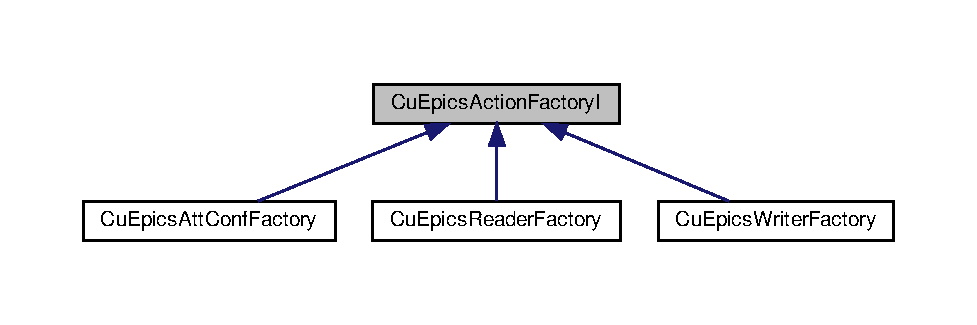
\includegraphics[width=350pt]{classCuEpicsActionFactoryI__inherit__graph}
\end{center}
\end{figure}
\subsection*{Public Member Functions}
\begin{DoxyCompactItemize}
\item 
\textbf{ Cu\+Epics\+Action\+FactoryI} ()
\item 
virtual \textbf{ Cu\+Epics\+ActionI} $\ast$ \textbf{ create} (const std\+::string \&source, \textbf{ Cumbia\+Epics} $\ast$ct) const =0
\item 
virtual \textbf{ Cu\+Epics\+Action\+I\+::\+Type} \textbf{ get\+Type} () const =0
\begin{DoxyCompactList}\small\item\em Return the type of action that the factory creates. \end{DoxyCompactList}\end{DoxyCompactItemize}


\subsection{Constructor \& Destructor Documentation}
\mbox{\label{classCuEpicsActionFactoryI_ae143654e9253d45fedddb91691f547b2}} 
\index{Cu\+Epics\+Action\+FactoryI@{Cu\+Epics\+Action\+FactoryI}!Cu\+Epics\+Action\+FactoryI@{Cu\+Epics\+Action\+FactoryI}}
\index{Cu\+Epics\+Action\+FactoryI@{Cu\+Epics\+Action\+FactoryI}!Cu\+Epics\+Action\+FactoryI@{Cu\+Epics\+Action\+FactoryI}}
\subsubsection{Cu\+Epics\+Action\+Factory\+I()}
{\footnotesize\ttfamily Cu\+Epics\+Action\+Factory\+I\+::\+Cu\+Epics\+Action\+FactoryI (\begin{DoxyParamCaption}{ }\end{DoxyParamCaption})\hspace{0.3cm}{\ttfamily [inline]}}



\subsection{Member Function Documentation}
\mbox{\label{classCuEpicsActionFactoryI_a37e60f748fad19a87626578f8badccf9}} 
\index{Cu\+Epics\+Action\+FactoryI@{Cu\+Epics\+Action\+FactoryI}!create@{create}}
\index{create@{create}!Cu\+Epics\+Action\+FactoryI@{Cu\+Epics\+Action\+FactoryI}}
\subsubsection{create()}
{\footnotesize\ttfamily virtual \textbf{ Cu\+Epics\+ActionI}$\ast$ Cu\+Epics\+Action\+Factory\+I\+::create (\begin{DoxyParamCaption}\item[{const std\+::string \&}]{source,  }\item[{\textbf{ Cumbia\+Epics} $\ast$}]{ct }\end{DoxyParamCaption}) const\hspace{0.3cm}{\ttfamily [pure virtual]}}



Implemented in \textbf{ Cu\+Epics\+Att\+Conf\+Factory} \doxyref{}{p.}{classCuEpicsAttConfFactory_ab44c19d1a61e57eb6044b46d616a3870}, \textbf{ Cu\+Epics\+Writer\+Factory} \doxyref{}{p.}{classCuEpicsWriterFactory_a5244cc75c1b4c4363506811c138d4411}, and \textbf{ Cu\+Epics\+Reader\+Factory} \doxyref{}{p.}{classCuEpicsReaderFactory_a935c44529bf2a9fd125093e95a1a476e}.



Referenced by Cu\+Action\+Factory\+Service\+::register\+Action().

\mbox{\label{classCuEpicsActionFactoryI_a8fe66bee4e67d957765071ef9d70815f}} 
\index{Cu\+Epics\+Action\+FactoryI@{Cu\+Epics\+Action\+FactoryI}!get\+Type@{get\+Type}}
\index{get\+Type@{get\+Type}!Cu\+Epics\+Action\+FactoryI@{Cu\+Epics\+Action\+FactoryI}}
\subsubsection{get\+Type()}
{\footnotesize\ttfamily virtual \textbf{ Cu\+Epics\+Action\+I\+::\+Type} Cu\+Epics\+Action\+Factory\+I\+::get\+Type (\begin{DoxyParamCaption}{ }\end{DoxyParamCaption}) const\hspace{0.3cm}{\ttfamily [pure virtual]}}



Return the type of action that the factory creates. 

\begin{DoxyReturn}{Returns}
the type of action that the factory creates 
\end{DoxyReturn}


Implemented in \textbf{ Cu\+Epics\+Att\+Conf\+Factory} \doxyref{}{p.}{classCuEpicsAttConfFactory_a5c7919a94d1f3d7362de21610ff9b480}, \textbf{ Cu\+Epics\+Writer\+Factory} \doxyref{}{p.}{classCuEpicsWriterFactory_a1c07cf03b37a3648240c5bddae90b669}, and \textbf{ Cu\+Epics\+Reader\+Factory} \doxyref{}{p.}{classCuEpicsReaderFactory_a2fae8622fb4054cfa0a829c341252e68}.



Referenced by Cumbia\+Epics\+::add\+Action(), and Cu\+Action\+Factory\+Service\+::register\+Action().



The documentation for this class was generated from the following file\+:\begin{DoxyCompactItemize}
\item 
\textbf{ cuepactionfactoryi.\+h}\end{DoxyCompactItemize}

\section{Cu\+Epics\+ActionI Class Reference}
\label{classCuEpicsActionI}\index{Cu\+Epics\+ActionI@{Cu\+Epics\+ActionI}}


an interface for an E\+P\+I\+CS {\itshape action}, as a reader (implemented) or a writer (not yet implemented)  




{\ttfamily \#include $<$cuepactioni.\+h$>$}



Inheritance diagram for Cu\+Epics\+ActionI\+:\nopagebreak
\begin{figure}[H]
\begin{center}
\leavevmode
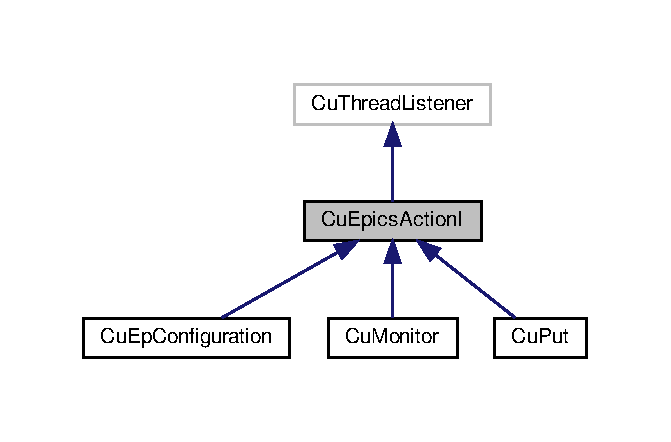
\includegraphics[width=322pt]{classCuEpicsActionI__inherit__graph}
\end{center}
\end{figure}
\subsection*{Public Types}
\begin{DoxyCompactItemize}
\item 
enum \textbf{ Type} \{ \newline
\textbf{ Reader} = 0, 
\textbf{ Writer}, 
\textbf{ Multi\+Reader}, 
\textbf{ Multi\+Writer}, 
\newline
\textbf{ Att\+Config}
 \}
\end{DoxyCompactItemize}
\subsection*{Public Member Functions}
\begin{DoxyCompactItemize}
\item 
virtual \textbf{ $\sim$\+Cu\+Epics\+ActionI} ()
\item 
virtual \textbf{ Ep\+Source} \textbf{ get\+Source} () const =0
\item 
virtual \textbf{ Type} \textbf{ get\+Type} () const =0
\item 
virtual void \textbf{ add\+Data\+Listener} (Cu\+Data\+Listener $\ast$l)=0
\item 
virtual void \textbf{ remove\+Data\+Listener} (Cu\+Data\+Listener $\ast$l)=0
\item 
virtual size\+\_\+t \textbf{ data\+Listeners\+Count} ()=0
\item 
virtual void \textbf{ start} ()=0
\item 
virtual void \textbf{ stop} ()=0
\item 
virtual void \textbf{ send\+Data} (const Cu\+Data \&data)=0
\item 
virtual void \textbf{ get\+Data} (Cu\+Data \&d\+\_\+inout) const =0
\end{DoxyCompactItemize}


\subsection{Detailed Description}
an interface for an E\+P\+I\+CS {\itshape action}, as a reader (implemented) or a writer (not yet implemented) 

A \doxyref{Cu\+Epics\+ActionI}{p.}{classCuEpicsActionI} describes what readers or writers usually do. They do {\itshape actions}, and they must adhere to this interface that requires to

\begin{DoxyItemize}
\item add or remove data listeners, that are updated by Cu\+Thread\+Listener\+::on\+Progress and Cu\+Thread\+Listener\+::on\+Result \item declare the type of action (Reader, Writer, ... -\/ see the Type enum) \item provide a start and a stop method where activities are instantiated and registered with Cumbia\+::register\+Activity and finally unregistered with Cumbia\+::unregister\+Activity \item provide an exiting method\end{DoxyItemize}
\begin{DoxyParagraph}{Examples}
\doxyref{Cu\+Monitor}{p.}{classCuMonitor} 
\end{DoxyParagraph}


\subsection{Member Enumeration Documentation}
\mbox{\label{classCuEpicsActionI_a6aa242a78ab0923128ee7240e8cb4996}} 
\index{Cu\+Epics\+ActionI@{Cu\+Epics\+ActionI}!Type@{Type}}
\index{Type@{Type}!Cu\+Epics\+ActionI@{Cu\+Epics\+ActionI}}
\subsubsection{Type}
{\footnotesize\ttfamily enum \textbf{ Cu\+Epics\+Action\+I\+::\+Type}}

\begin{DoxyEnumFields}{Enumerator}
\raisebox{\heightof{T}}[0pt][0pt]{\index{Reader@{Reader}!Cu\+Epics\+ActionI@{Cu\+Epics\+ActionI}}\index{Cu\+Epics\+ActionI@{Cu\+Epics\+ActionI}!Reader@{Reader}}}\mbox{\label{classCuEpicsActionI_a6aa242a78ab0923128ee7240e8cb4996abec6454a2228324af9a9a8d609139eea}} 
Reader&\\
\hline

\raisebox{\heightof{T}}[0pt][0pt]{\index{Writer@{Writer}!Cu\+Epics\+ActionI@{Cu\+Epics\+ActionI}}\index{Cu\+Epics\+ActionI@{Cu\+Epics\+ActionI}!Writer@{Writer}}}\mbox{\label{classCuEpicsActionI_a6aa242a78ab0923128ee7240e8cb4996a2814e834b6118236b30b68e1b1a09892}} 
Writer&\\
\hline

\raisebox{\heightof{T}}[0pt][0pt]{\index{Multi\+Reader@{Multi\+Reader}!Cu\+Epics\+ActionI@{Cu\+Epics\+ActionI}}\index{Cu\+Epics\+ActionI@{Cu\+Epics\+ActionI}!Multi\+Reader@{Multi\+Reader}}}\mbox{\label{classCuEpicsActionI_a6aa242a78ab0923128ee7240e8cb4996abe95488059ac6b8ffda43188e8f3c25c}} 
Multi\+Reader&\\
\hline

\raisebox{\heightof{T}}[0pt][0pt]{\index{Multi\+Writer@{Multi\+Writer}!Cu\+Epics\+ActionI@{Cu\+Epics\+ActionI}}\index{Cu\+Epics\+ActionI@{Cu\+Epics\+ActionI}!Multi\+Writer@{Multi\+Writer}}}\mbox{\label{classCuEpicsActionI_a6aa242a78ab0923128ee7240e8cb4996a7e4de54ba7d4989a3f9cda912497eda9}} 
Multi\+Writer&\\
\hline

\raisebox{\heightof{T}}[0pt][0pt]{\index{Att\+Config@{Att\+Config}!Cu\+Epics\+ActionI@{Cu\+Epics\+ActionI}}\index{Cu\+Epics\+ActionI@{Cu\+Epics\+ActionI}!Att\+Config@{Att\+Config}}}\mbox{\label{classCuEpicsActionI_a6aa242a78ab0923128ee7240e8cb4996a68151bef7b6137ea7871d96d1d9db3dc}} 
Att\+Config&\\
\hline

\end{DoxyEnumFields}


\subsection{Constructor \& Destructor Documentation}
\mbox{\label{classCuEpicsActionI_a7bcac707951c151e690c10bfed969408}} 
\index{Cu\+Epics\+ActionI@{Cu\+Epics\+ActionI}!````~Cu\+Epics\+ActionI@{$\sim$\+Cu\+Epics\+ActionI}}
\index{````~Cu\+Epics\+ActionI@{$\sim$\+Cu\+Epics\+ActionI}!Cu\+Epics\+ActionI@{Cu\+Epics\+ActionI}}
\subsubsection{$\sim$\+Cu\+Epics\+Action\+I()}
{\footnotesize\ttfamily virtual Cu\+Epics\+Action\+I\+::$\sim$\+Cu\+Epics\+ActionI (\begin{DoxyParamCaption}{ }\end{DoxyParamCaption})\hspace{0.3cm}{\ttfamily [inline]}, {\ttfamily [virtual]}}



\subsection{Member Function Documentation}
\mbox{\label{classCuEpicsActionI_a8e6c0261f02cb237d612e097fee6dc4a}} 
\index{Cu\+Epics\+ActionI@{Cu\+Epics\+ActionI}!add\+Data\+Listener@{add\+Data\+Listener}}
\index{add\+Data\+Listener@{add\+Data\+Listener}!Cu\+Epics\+ActionI@{Cu\+Epics\+ActionI}}
\subsubsection{add\+Data\+Listener()}
{\footnotesize\ttfamily virtual void Cu\+Epics\+Action\+I\+::add\+Data\+Listener (\begin{DoxyParamCaption}\item[{Cu\+Data\+Listener $\ast$}]{l }\end{DoxyParamCaption})\hspace{0.3cm}{\ttfamily [pure virtual]}}



Implemented in \textbf{ Cu\+Monitor} \doxyref{}{p.}{classCuMonitor_ac82feb2bd46c4a7b80c8803d8c2716e9}, \textbf{ Cu\+Ep\+Configuration} \doxyref{}{p.}{classCuEpConfiguration_a4f89b2a4514f6d8135d7c2e0c0b626dd}, and \textbf{ Cu\+Put} \doxyref{}{p.}{classCuPut_a304735be4bbef6c03d30862dd69e9213}.



Referenced by Cumbia\+Epics\+::add\+Action().

\mbox{\label{classCuEpicsActionI_af7b509410aaee059c3105dfb10b33ee7}} 
\index{Cu\+Epics\+ActionI@{Cu\+Epics\+ActionI}!data\+Listeners\+Count@{data\+Listeners\+Count}}
\index{data\+Listeners\+Count@{data\+Listeners\+Count}!Cu\+Epics\+ActionI@{Cu\+Epics\+ActionI}}
\subsubsection{data\+Listeners\+Count()}
{\footnotesize\ttfamily virtual size\+\_\+t Cu\+Epics\+Action\+I\+::data\+Listeners\+Count (\begin{DoxyParamCaption}{ }\end{DoxyParamCaption})\hspace{0.3cm}{\ttfamily [pure virtual]}}



Implemented in \textbf{ Cu\+Monitor} \doxyref{}{p.}{classCuMonitor_a269325e57d5e989c8904ebb12614db43}, \textbf{ Cu\+Ep\+Configuration} \doxyref{}{p.}{classCuEpConfiguration_ad7c394d3a0b0881091cb7c918b7fd1cf}, and \textbf{ Cu\+Put} \doxyref{}{p.}{classCuPut_ac342b254939cd2fc532210fd1ec55c1e}.

\mbox{\label{classCuEpicsActionI_a063d9436f8a6b84a22a384d06c3996bd}} 
\index{Cu\+Epics\+ActionI@{Cu\+Epics\+ActionI}!get\+Data@{get\+Data}}
\index{get\+Data@{get\+Data}!Cu\+Epics\+ActionI@{Cu\+Epics\+ActionI}}
\subsubsection{get\+Data()}
{\footnotesize\ttfamily virtual void Cu\+Epics\+Action\+I\+::get\+Data (\begin{DoxyParamCaption}\item[{Cu\+Data \&}]{d\+\_\+inout }\end{DoxyParamCaption}) const\hspace{0.3cm}{\ttfamily [pure virtual]}}



Implemented in \textbf{ Cu\+Monitor} \doxyref{}{p.}{classCuMonitor_aceebd11ad99f54e64538bd1620377869}, \textbf{ Cu\+Put} \doxyref{}{p.}{classCuPut_a12b24fa9a83564254812fb29c169dfd9}, and \textbf{ Cu\+Ep\+Configuration} \doxyref{}{p.}{classCuEpConfiguration_a1941fa5e0812068058b17cf9f9827c4d}.

\mbox{\label{classCuEpicsActionI_a2c97ba6d9bbd9e98fec51aa92d2becb6}} 
\index{Cu\+Epics\+ActionI@{Cu\+Epics\+ActionI}!get\+Source@{get\+Source}}
\index{get\+Source@{get\+Source}!Cu\+Epics\+ActionI@{Cu\+Epics\+ActionI}}
\subsubsection{get\+Source()}
{\footnotesize\ttfamily virtual \textbf{ Ep\+Source} Cu\+Epics\+Action\+I\+::get\+Source (\begin{DoxyParamCaption}{ }\end{DoxyParamCaption}) const\hspace{0.3cm}{\ttfamily [pure virtual]}}



Implemented in \textbf{ Cu\+Monitor} \doxyref{}{p.}{classCuMonitor_ae904ab4e124c106476a552cc982e07e6}, \textbf{ Cu\+Ep\+Configuration} \doxyref{}{p.}{classCuEpConfiguration_a3fdc803bd3890ec9a39486ae5e7382b3}, and \textbf{ Cu\+Put} \doxyref{}{p.}{classCuPut_a7ede2832b45255e30fae59388f0873b4}.

\mbox{\label{classCuEpicsActionI_a7386456fda8f1fe44dac1960842b96a6}} 
\index{Cu\+Epics\+ActionI@{Cu\+Epics\+ActionI}!get\+Type@{get\+Type}}
\index{get\+Type@{get\+Type}!Cu\+Epics\+ActionI@{Cu\+Epics\+ActionI}}
\subsubsection{get\+Type()}
{\footnotesize\ttfamily virtual \textbf{ Type} Cu\+Epics\+Action\+I\+::get\+Type (\begin{DoxyParamCaption}{ }\end{DoxyParamCaption}) const\hspace{0.3cm}{\ttfamily [pure virtual]}}



Implemented in \textbf{ Cu\+Monitor} \doxyref{}{p.}{classCuMonitor_acaffe461ab729a2a0af48a4c77a94292}, \textbf{ Cu\+Ep\+Configuration} \doxyref{}{p.}{classCuEpConfiguration_afe9b397877ed5311df2176244ca5112f}, and \textbf{ Cu\+Put} \doxyref{}{p.}{classCuPut_aace1d281b4a27ee445aa023ce0d12483}.

\mbox{\label{classCuEpicsActionI_a5f5c5045ae8f93ed95794538c495dfdf}} 
\index{Cu\+Epics\+ActionI@{Cu\+Epics\+ActionI}!remove\+Data\+Listener@{remove\+Data\+Listener}}
\index{remove\+Data\+Listener@{remove\+Data\+Listener}!Cu\+Epics\+ActionI@{Cu\+Epics\+ActionI}}
\subsubsection{remove\+Data\+Listener()}
{\footnotesize\ttfamily virtual void Cu\+Epics\+Action\+I\+::remove\+Data\+Listener (\begin{DoxyParamCaption}\item[{Cu\+Data\+Listener $\ast$}]{l }\end{DoxyParamCaption})\hspace{0.3cm}{\ttfamily [pure virtual]}}



Implemented in \textbf{ Cu\+Monitor} \doxyref{}{p.}{classCuMonitor_a5b4b77c29cfb45591f4e4a486c8e5000}, \textbf{ Cu\+Ep\+Configuration} \doxyref{}{p.}{classCuEpConfiguration_a45ceb248426de776e465bf06ce94e042}, and \textbf{ Cu\+Put} \doxyref{}{p.}{classCuPut_aea881574b86c093293ea4b16749aa187}.



Referenced by Cumbia\+Epics\+::unlink\+Listener().

\mbox{\label{classCuEpicsActionI_acced5eb52ec2b30b2f21ca30b043d683}} 
\index{Cu\+Epics\+ActionI@{Cu\+Epics\+ActionI}!send\+Data@{send\+Data}}
\index{send\+Data@{send\+Data}!Cu\+Epics\+ActionI@{Cu\+Epics\+ActionI}}
\subsubsection{send\+Data()}
{\footnotesize\ttfamily virtual void Cu\+Epics\+Action\+I\+::send\+Data (\begin{DoxyParamCaption}\item[{const Cu\+Data \&}]{data }\end{DoxyParamCaption})\hspace{0.3cm}{\ttfamily [pure virtual]}}



Implemented in \textbf{ Cu\+Monitor} \doxyref{}{p.}{classCuMonitor_ad40b612c2d9b8864d92523a40e5e663a}, \textbf{ Cu\+Put} \doxyref{}{p.}{classCuPut_aa157f27047f346c478acb8f7bd64f818}, and \textbf{ Cu\+Ep\+Configuration} \doxyref{}{p.}{classCuEpConfiguration_ad40463466a0d3f298c2bc155115ffcd8}.

\mbox{\label{classCuEpicsActionI_aa6b252261a7763d5e4266b9a68042cac}} 
\index{Cu\+Epics\+ActionI@{Cu\+Epics\+ActionI}!start@{start}}
\index{start@{start}!Cu\+Epics\+ActionI@{Cu\+Epics\+ActionI}}
\subsubsection{start()}
{\footnotesize\ttfamily void Cu\+Epics\+Action\+I\+::start (\begin{DoxyParamCaption}{ }\end{DoxyParamCaption})\hspace{0.3cm}{\ttfamily [pure virtual]}}



Implemented in \textbf{ Cu\+Monitor} \doxyref{}{p.}{classCuMonitor_a120832bff1f21fab34cf3a4bcf43af60}, \textbf{ Cu\+Ep\+Configuration} \doxyref{}{p.}{classCuEpConfiguration_a322fd687e6c2ee0e33b9e8a7b1b0bead}, and \textbf{ Cu\+Put} \doxyref{}{p.}{classCuPut_a6f22cba2a2d20376c912d017eeb09236}.



Referenced by Cumbia\+Epics\+::add\+Action().

\mbox{\label{classCuEpicsActionI_adf2f365700c5cc859929db4495216323}} 
\index{Cu\+Epics\+ActionI@{Cu\+Epics\+ActionI}!stop@{stop}}
\index{stop@{stop}!Cu\+Epics\+ActionI@{Cu\+Epics\+ActionI}}
\subsubsection{stop()}
{\footnotesize\ttfamily void Cu\+Epics\+Action\+I\+::stop (\begin{DoxyParamCaption}{ }\end{DoxyParamCaption})\hspace{0.3cm}{\ttfamily [pure virtual]}}



Implemented in \textbf{ Cu\+Monitor} \doxyref{}{p.}{classCuMonitor_a03599f48c24d5f9ba63304a0f03cb144}, \textbf{ Cu\+Ep\+Configuration} \doxyref{}{p.}{classCuEpConfiguration_aba9655517430a9bc4c9dd41ff9eb6ba7}, and \textbf{ Cu\+Put} \doxyref{}{p.}{classCuPut_a04c85dea0e8c18f0ba4ee6b572848b8a}.



The documentation for this class was generated from the following files\+:\begin{DoxyCompactItemize}
\item 
\textbf{ cuepactioni.\+h}\item 
\textbf{ cuepactioni.\+cpp}\end{DoxyCompactItemize}

\section{Cu\+Epics\+Att\+Conf\+Factory Class Reference}
\label{classCuEpicsAttConfFactory}\index{Cu\+Epics\+Att\+Conf\+Factory@{Cu\+Epics\+Att\+Conf\+Factory}}


{\ttfamily \#include $<$cuepactionfactories.\+h$>$}



Inheritance diagram for Cu\+Epics\+Att\+Conf\+Factory\+:\nopagebreak
\begin{figure}[H]
\begin{center}
\leavevmode
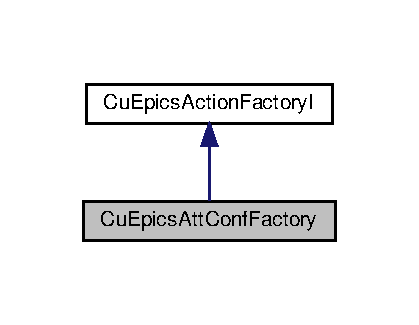
\includegraphics[width=201pt]{classCuEpicsAttConfFactory__inherit__graph}
\end{center}
\end{figure}
\subsection*{Public Member Functions}
\begin{DoxyCompactItemize}
\item 
\textbf{ Cu\+Epics\+Att\+Conf\+Factory} ()
\item 
void \textbf{ fetch\+Attribute\+History} (bool fetch)
\item 
void \textbf{ set\+Desired\+Attribute\+Properties} (const std\+::vector$<$ std\+::string $>$ props)
\item 
\textbf{ Cu\+Epics\+ActionI} $\ast$ \textbf{ create} (const std\+::string \&s, \textbf{ Cumbia\+Epics} $\ast$ct) const
\item 
\textbf{ Cu\+Epics\+Action\+I\+::\+Type} \textbf{ get\+Type} () const
\begin{DoxyCompactList}\small\item\em Return the type of action that the factory creates. \end{DoxyCompactList}\end{DoxyCompactItemize}


\subsection{Constructor \& Destructor Documentation}
\mbox{\label{classCuEpicsAttConfFactory_abe7be55c604a2cac2b67bd060d56b219}} 
\index{Cu\+Epics\+Att\+Conf\+Factory@{Cu\+Epics\+Att\+Conf\+Factory}!Cu\+Epics\+Att\+Conf\+Factory@{Cu\+Epics\+Att\+Conf\+Factory}}
\index{Cu\+Epics\+Att\+Conf\+Factory@{Cu\+Epics\+Att\+Conf\+Factory}!Cu\+Epics\+Att\+Conf\+Factory@{Cu\+Epics\+Att\+Conf\+Factory}}
\subsubsection{Cu\+Epics\+Att\+Conf\+Factory()}
{\footnotesize\ttfamily Cu\+Epics\+Att\+Conf\+Factory\+::\+Cu\+Epics\+Att\+Conf\+Factory (\begin{DoxyParamCaption}{ }\end{DoxyParamCaption})}



\subsection{Member Function Documentation}
\mbox{\label{classCuEpicsAttConfFactory_ab44c19d1a61e57eb6044b46d616a3870}} 
\index{Cu\+Epics\+Att\+Conf\+Factory@{Cu\+Epics\+Att\+Conf\+Factory}!create@{create}}
\index{create@{create}!Cu\+Epics\+Att\+Conf\+Factory@{Cu\+Epics\+Att\+Conf\+Factory}}
\subsubsection{create()}
{\footnotesize\ttfamily \textbf{ Cu\+Epics\+ActionI} $\ast$ Cu\+Epics\+Att\+Conf\+Factory\+::create (\begin{DoxyParamCaption}\item[{const std\+::string \&}]{s,  }\item[{\textbf{ Cumbia\+Epics} $\ast$}]{ct }\end{DoxyParamCaption}) const\hspace{0.3cm}{\ttfamily [virtual]}}



Implements \textbf{ Cu\+Epics\+Action\+FactoryI} \doxyref{}{p.}{classCuEpicsActionFactoryI_a37e60f748fad19a87626578f8badccf9}.



References Cu\+Ep\+Configuration\+::set\+Desired\+Attribute\+Properties().

\mbox{\label{classCuEpicsAttConfFactory_ab7e1293f4b38ea52547de4feb98783d2}} 
\index{Cu\+Epics\+Att\+Conf\+Factory@{Cu\+Epics\+Att\+Conf\+Factory}!fetch\+Attribute\+History@{fetch\+Attribute\+History}}
\index{fetch\+Attribute\+History@{fetch\+Attribute\+History}!Cu\+Epics\+Att\+Conf\+Factory@{Cu\+Epics\+Att\+Conf\+Factory}}
\subsubsection{fetch\+Attribute\+History()}
{\footnotesize\ttfamily void Cu\+Epics\+Att\+Conf\+Factory\+::fetch\+Attribute\+History (\begin{DoxyParamCaption}\item[{bool}]{fetch }\end{DoxyParamCaption})}

\mbox{\label{classCuEpicsAttConfFactory_a5c7919a94d1f3d7362de21610ff9b480}} 
\index{Cu\+Epics\+Att\+Conf\+Factory@{Cu\+Epics\+Att\+Conf\+Factory}!get\+Type@{get\+Type}}
\index{get\+Type@{get\+Type}!Cu\+Epics\+Att\+Conf\+Factory@{Cu\+Epics\+Att\+Conf\+Factory}}
\subsubsection{get\+Type()}
{\footnotesize\ttfamily \textbf{ Cu\+Epics\+Action\+I\+::\+Type} Cu\+Epics\+Att\+Conf\+Factory\+::get\+Type (\begin{DoxyParamCaption}{ }\end{DoxyParamCaption}) const\hspace{0.3cm}{\ttfamily [virtual]}}



Return the type of action that the factory creates. 

\begin{DoxyReturn}{Returns}
the type of action that the factory creates 
\end{DoxyReturn}


Implements \textbf{ Cu\+Epics\+Action\+FactoryI} \doxyref{}{p.}{classCuEpicsActionFactoryI_a8fe66bee4e67d957765071ef9d70815f}.



References Cu\+Epics\+Action\+I\+::\+Att\+Config.

\mbox{\label{classCuEpicsAttConfFactory_ae03e4f3a2b8a3cfe3be164ec62d80e34}} 
\index{Cu\+Epics\+Att\+Conf\+Factory@{Cu\+Epics\+Att\+Conf\+Factory}!set\+Desired\+Attribute\+Properties@{set\+Desired\+Attribute\+Properties}}
\index{set\+Desired\+Attribute\+Properties@{set\+Desired\+Attribute\+Properties}!Cu\+Epics\+Att\+Conf\+Factory@{Cu\+Epics\+Att\+Conf\+Factory}}
\subsubsection{set\+Desired\+Attribute\+Properties()}
{\footnotesize\ttfamily void Cu\+Epics\+Att\+Conf\+Factory\+::set\+Desired\+Attribute\+Properties (\begin{DoxyParamCaption}\item[{const std\+::vector$<$ std\+::string $>$}]{props }\end{DoxyParamCaption})}



The documentation for this class was generated from the following files\+:\begin{DoxyCompactItemize}
\item 
\textbf{ cuepactionfactories.\+h}\item 
\textbf{ cuepactionfactories.\+cpp}\end{DoxyCompactItemize}

\section{Cu\+Epics\+Reader\+Factory Class Reference}
\label{classCuEpicsReaderFactory}\index{Cu\+Epics\+Reader\+Factory@{Cu\+Epics\+Reader\+Factory}}


{\ttfamily \#include $<$cuepactionfactories.\+h$>$}



Inheritance diagram for Cu\+Epics\+Reader\+Factory\+:\nopagebreak
\begin{figure}[H]
\begin{center}
\leavevmode
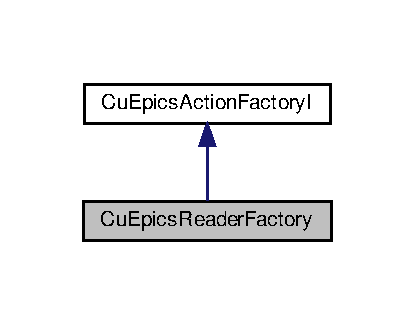
\includegraphics[width=199pt]{classCuEpicsReaderFactory__inherit__graph}
\end{center}
\end{figure}
\subsection*{Public Member Functions}
\begin{DoxyCompactItemize}
\item 
\textbf{ Cu\+Epics\+Reader\+Factory} ()
\item 
void \textbf{ set\+Options} (const Cu\+Data \&o)
\item 
virtual \textbf{ $\sim$\+Cu\+Epics\+Reader\+Factory} ()
\item 
\textbf{ Cu\+Epics\+ActionI} $\ast$ \textbf{ create} (const std\+::string \&s, \textbf{ Cumbia\+Epics} $\ast$ct) const
\item 
\textbf{ Cu\+Epics\+Action\+I\+::\+Type} \textbf{ get\+Type} () const
\begin{DoxyCompactList}\small\item\em Return the type of action that the factory creates. \end{DoxyCompactList}\item 
bool \textbf{ is\+Shareable} () const
\end{DoxyCompactItemize}


\subsection{Constructor \& Destructor Documentation}
\mbox{\label{classCuEpicsReaderFactory_abced8817bd86b9dc6aeb50a39961f2a6}} 
\index{Cu\+Epics\+Reader\+Factory@{Cu\+Epics\+Reader\+Factory}!Cu\+Epics\+Reader\+Factory@{Cu\+Epics\+Reader\+Factory}}
\index{Cu\+Epics\+Reader\+Factory@{Cu\+Epics\+Reader\+Factory}!Cu\+Epics\+Reader\+Factory@{Cu\+Epics\+Reader\+Factory}}
\subsubsection{Cu\+Epics\+Reader\+Factory()}
{\footnotesize\ttfamily Cu\+Epics\+Reader\+Factory\+::\+Cu\+Epics\+Reader\+Factory (\begin{DoxyParamCaption}{ }\end{DoxyParamCaption})}



References Cu\+Monitor\+::\+Monitor\+Refresh.

\mbox{\label{classCuEpicsReaderFactory_a63f8295819398ebead164fb6fb31c75f}} 
\index{Cu\+Epics\+Reader\+Factory@{Cu\+Epics\+Reader\+Factory}!````~Cu\+Epics\+Reader\+Factory@{$\sim$\+Cu\+Epics\+Reader\+Factory}}
\index{````~Cu\+Epics\+Reader\+Factory@{$\sim$\+Cu\+Epics\+Reader\+Factory}!Cu\+Epics\+Reader\+Factory@{Cu\+Epics\+Reader\+Factory}}
\subsubsection{$\sim$\+Cu\+Epics\+Reader\+Factory()}
{\footnotesize\ttfamily Cu\+Epics\+Reader\+Factory\+::$\sim$\+Cu\+Epics\+Reader\+Factory (\begin{DoxyParamCaption}{ }\end{DoxyParamCaption})\hspace{0.3cm}{\ttfamily [virtual]}}



\subsection{Member Function Documentation}
\mbox{\label{classCuEpicsReaderFactory_a935c44529bf2a9fd125093e95a1a476e}} 
\index{Cu\+Epics\+Reader\+Factory@{Cu\+Epics\+Reader\+Factory}!create@{create}}
\index{create@{create}!Cu\+Epics\+Reader\+Factory@{Cu\+Epics\+Reader\+Factory}}
\subsubsection{create()}
{\footnotesize\ttfamily \textbf{ Cu\+Epics\+ActionI} $\ast$ Cu\+Epics\+Reader\+Factory\+::create (\begin{DoxyParamCaption}\item[{const std\+::string \&}]{s,  }\item[{\textbf{ Cumbia\+Epics} $\ast$}]{ct }\end{DoxyParamCaption}) const\hspace{0.3cm}{\ttfamily [virtual]}}



Implements \textbf{ Cu\+Epics\+Action\+FactoryI} \doxyref{}{p.}{classCuEpicsActionFactoryI_a37e60f748fad19a87626578f8badccf9}.



References Cu\+Monitor\+::set\+Period(), and Cu\+Monitor\+::set\+Refresh\+Mode().

\mbox{\label{classCuEpicsReaderFactory_a2fae8622fb4054cfa0a829c341252e68}} 
\index{Cu\+Epics\+Reader\+Factory@{Cu\+Epics\+Reader\+Factory}!get\+Type@{get\+Type}}
\index{get\+Type@{get\+Type}!Cu\+Epics\+Reader\+Factory@{Cu\+Epics\+Reader\+Factory}}
\subsubsection{get\+Type()}
{\footnotesize\ttfamily \textbf{ Cu\+Epics\+Action\+I\+::\+Type} Cu\+Epics\+Reader\+Factory\+::get\+Type (\begin{DoxyParamCaption}{ }\end{DoxyParamCaption}) const\hspace{0.3cm}{\ttfamily [virtual]}}



Return the type of action that the factory creates. 

\begin{DoxyReturn}{Returns}
the type of action that the factory creates 
\end{DoxyReturn}


Implements \textbf{ Cu\+Epics\+Action\+FactoryI} \doxyref{}{p.}{classCuEpicsActionFactoryI_a8fe66bee4e67d957765071ef9d70815f}.



References Cu\+Epics\+Action\+I\+::\+Reader.

\mbox{\label{classCuEpicsReaderFactory_ab5e57e41c757ded3f35cd861633e0ab2}} 
\index{Cu\+Epics\+Reader\+Factory@{Cu\+Epics\+Reader\+Factory}!is\+Shareable@{is\+Shareable}}
\index{is\+Shareable@{is\+Shareable}!Cu\+Epics\+Reader\+Factory@{Cu\+Epics\+Reader\+Factory}}
\subsubsection{is\+Shareable()}
{\footnotesize\ttfamily bool Cu\+Epics\+Reader\+Factory\+::is\+Shareable (\begin{DoxyParamCaption}{ }\end{DoxyParamCaption}) const}

\mbox{\label{classCuEpicsReaderFactory_a12a4143e8e7f27778ebfa27d76e0f6c9}} 
\index{Cu\+Epics\+Reader\+Factory@{Cu\+Epics\+Reader\+Factory}!set\+Options@{set\+Options}}
\index{set\+Options@{set\+Options}!Cu\+Epics\+Reader\+Factory@{Cu\+Epics\+Reader\+Factory}}
\subsubsection{set\+Options()}
{\footnotesize\ttfamily void Cu\+Epics\+Reader\+Factory\+::set\+Options (\begin{DoxyParamCaption}\item[{const Cu\+Data \&}]{o }\end{DoxyParamCaption})}



The documentation for this class was generated from the following files\+:\begin{DoxyCompactItemize}
\item 
\textbf{ cuepactionfactories.\+h}\item 
\textbf{ cuepactionfactories.\+cpp}\end{DoxyCompactItemize}

\section{Cu\+Epics\+Read\+Options Class Reference}
\label{classCuEpicsReadOptions}\index{Cu\+Epics\+Read\+Options@{Cu\+Epics\+Read\+Options}}


{\ttfamily \#include $<$cuepreadoptions.\+h$>$}

\subsection*{Public Member Functions}
\begin{DoxyCompactItemize}
\item 
\textbf{ Cu\+Epics\+Read\+Options} ()
\item 
\textbf{ Cu\+Epics\+Read\+Options} (int per, \textbf{ Cu\+Monitor\+::\+Refresh\+Mode} mod)
\end{DoxyCompactItemize}
\subsection*{Public Attributes}
\begin{DoxyCompactItemize}
\item 
int \textbf{ period}
\item 
\textbf{ Cu\+Monitor\+::\+Refresh\+Mode} \textbf{ mode}
\end{DoxyCompactItemize}


\subsection{Constructor \& Destructor Documentation}
\mbox{\label{classCuEpicsReadOptions_a5dbf0709cac6c214535b27393ff497d2}} 
\index{Cu\+Epics\+Read\+Options@{Cu\+Epics\+Read\+Options}!Cu\+Epics\+Read\+Options@{Cu\+Epics\+Read\+Options}}
\index{Cu\+Epics\+Read\+Options@{Cu\+Epics\+Read\+Options}!Cu\+Epics\+Read\+Options@{Cu\+Epics\+Read\+Options}}
\subsubsection{Cu\+Epics\+Read\+Options()\hspace{0.1cm}{\footnotesize\ttfamily [1/2]}}
{\footnotesize\ttfamily Cu\+Epics\+Read\+Options\+::\+Cu\+Epics\+Read\+Options (\begin{DoxyParamCaption}{ }\end{DoxyParamCaption})}



References mode, Cu\+Monitor\+::\+Monitor\+Refresh, and period.

\mbox{\label{classCuEpicsReadOptions_a400ad3c4dc95bed995b2ab07c939b1eb}} 
\index{Cu\+Epics\+Read\+Options@{Cu\+Epics\+Read\+Options}!Cu\+Epics\+Read\+Options@{Cu\+Epics\+Read\+Options}}
\index{Cu\+Epics\+Read\+Options@{Cu\+Epics\+Read\+Options}!Cu\+Epics\+Read\+Options@{Cu\+Epics\+Read\+Options}}
\subsubsection{Cu\+Epics\+Read\+Options()\hspace{0.1cm}{\footnotesize\ttfamily [2/2]}}
{\footnotesize\ttfamily Cu\+Epics\+Read\+Options\+::\+Cu\+Epics\+Read\+Options (\begin{DoxyParamCaption}\item[{int}]{per,  }\item[{\textbf{ Cu\+Monitor\+::\+Refresh\+Mode}}]{mod }\end{DoxyParamCaption})}



References mode, and period.



\subsection{Member Data Documentation}
\mbox{\label{classCuEpicsReadOptions_a5d89b8bae8dc8196563396104f867dbd}} 
\index{Cu\+Epics\+Read\+Options@{Cu\+Epics\+Read\+Options}!mode@{mode}}
\index{mode@{mode}!Cu\+Epics\+Read\+Options@{Cu\+Epics\+Read\+Options}}
\subsubsection{mode}
{\footnotesize\ttfamily \textbf{ Cu\+Monitor\+::\+Refresh\+Mode} Cu\+Epics\+Read\+Options\+::mode}



Referenced by Cu\+Epics\+Read\+Options().

\mbox{\label{classCuEpicsReadOptions_aeef25d2ce0802fa8c763863827710098}} 
\index{Cu\+Epics\+Read\+Options@{Cu\+Epics\+Read\+Options}!period@{period}}
\index{period@{period}!Cu\+Epics\+Read\+Options@{Cu\+Epics\+Read\+Options}}
\subsubsection{period}
{\footnotesize\ttfamily int Cu\+Epics\+Read\+Options\+::period}



Referenced by Cu\+Epics\+Read\+Options().



The documentation for this class was generated from the following files\+:\begin{DoxyCompactItemize}
\item 
\textbf{ cuepreadoptions.\+h}\item 
\textbf{ cuepreadoptions.\+cpp}\end{DoxyCompactItemize}

\section{Cu\+Epics\+World Class Reference}
\label{classCuEpicsWorld}\index{Cu\+Epics\+World@{Cu\+Epics\+World}}


{\ttfamily \#include $<$cuepics-\/world.\+h$>$}

\subsection*{Public Member Functions}
\begin{DoxyCompactItemize}
\item 
\textbf{ Cu\+Epics\+World} ()
\item 
virtual \textbf{ $\sim$\+Cu\+Epics\+World} ()
\item 
std\+::string \textbf{ get\+Last\+Message} () const
\item 
void \textbf{ fill\+Thread\+Info} (Cu\+Data \&d, const Cu\+Activity $\ast$a)
\item 
bool \textbf{ error} () const
\item 
bool \textbf{ source\+\_\+valid} (const std\+::string \&s) const
\item 
void \textbf{ extract\+Data} (const \textbf{ Cu\+PV} $\ast$\+\_\+pv, Cu\+Data \&da) const
\item 
std\+::string \textbf{ extract\+Exception} (struct exception\+\_\+handler\+\_\+args excargs, Cu\+Data \&d) const
\begin{DoxyCompactList}\small\item\em fills the input Cu\+Data with exception information. \end{DoxyCompactList}\item 
{\footnotesize template$<$class T $>$ }\\void \textbf{ put\+Timestamp} (void $\ast$ep\+\_\+data, Cu\+Data \&d) const
\item 
{\footnotesize template$<$class T $>$ }\\void \textbf{ put\+Ctrl\+Data} (void $\ast$ep\+\_\+data, Cu\+Data \&d) const
\item 
void \textbf{ set\+Src\+Patterns} (const std\+::vector$<$ std\+::string $>$ \&p)
\item 
std\+::vector$<$ std\+::string $>$ \textbf{ src\+Patterns} () const
\end{DoxyCompactItemize}


\subsection{Constructor \& Destructor Documentation}
\mbox{\label{classCuEpicsWorld_ab42c206f9bad4e5491052ddeda4ac773}} 
\index{Cu\+Epics\+World@{Cu\+Epics\+World}!Cu\+Epics\+World@{Cu\+Epics\+World}}
\index{Cu\+Epics\+World@{Cu\+Epics\+World}!Cu\+Epics\+World@{Cu\+Epics\+World}}
\subsubsection{Cu\+Epics\+World()}
{\footnotesize\ttfamily Cu\+Epics\+World\+::\+Cu\+Epics\+World (\begin{DoxyParamCaption}{ }\end{DoxyParamCaption})}



References Cu\+Epics\+World\+Private\+::src\+\_\+patterns.

\mbox{\label{classCuEpicsWorld_a48e6dc05f7b79752047a3cf20ea4b61b}} 
\index{Cu\+Epics\+World@{Cu\+Epics\+World}!````~Cu\+Epics\+World@{$\sim$\+Cu\+Epics\+World}}
\index{````~Cu\+Epics\+World@{$\sim$\+Cu\+Epics\+World}!Cu\+Epics\+World@{Cu\+Epics\+World}}
\subsubsection{$\sim$\+Cu\+Epics\+World()}
{\footnotesize\ttfamily Cu\+Epics\+World\+::$\sim$\+Cu\+Epics\+World (\begin{DoxyParamCaption}{ }\end{DoxyParamCaption})\hspace{0.3cm}{\ttfamily [virtual]}}



\subsection{Member Function Documentation}
\mbox{\label{classCuEpicsWorld_a01c2f45af889d0bf2f2a1f0dae877624}} 
\index{Cu\+Epics\+World@{Cu\+Epics\+World}!error@{error}}
\index{error@{error}!Cu\+Epics\+World@{Cu\+Epics\+World}}
\subsubsection{error()}
{\footnotesize\ttfamily bool Cu\+Epics\+World\+::error (\begin{DoxyParamCaption}{ }\end{DoxyParamCaption}) const}



References Cu\+Epics\+World\+Private\+::error.



Referenced by Cu\+Monitor\+Activity\+::event\+\_\+handler().

\mbox{\label{classCuEpicsWorld_ada0feac3aef6923b41d9913664d96e88}} 
\index{Cu\+Epics\+World@{Cu\+Epics\+World}!extract\+Data@{extract\+Data}}
\index{extract\+Data@{extract\+Data}!Cu\+Epics\+World@{Cu\+Epics\+World}}
\subsubsection{extract\+Data()}
{\footnotesize\ttfamily void Cu\+Epics\+World\+::extract\+Data (\begin{DoxyParamCaption}\item[{const \textbf{ Cu\+PV} $\ast$}]{\+\_\+pv,  }\item[{Cu\+Data \&}]{da }\end{DoxyParamCaption}) const}



References Cu\+P\+V\+::dbr\+Type, Cu\+Epics\+World\+Private\+::error, Cu\+Epics\+World\+Private\+::message, Cu\+P\+V\+::n\+Elems, and Cu\+P\+V\+::value.



Referenced by Cu\+Monitor\+Activity\+::event\+\_\+handler().

\mbox{\label{classCuEpicsWorld_aebd4c38ec2d510f69de4708fb0a7638c}} 
\index{Cu\+Epics\+World@{Cu\+Epics\+World}!extract\+Exception@{extract\+Exception}}
\index{extract\+Exception@{extract\+Exception}!Cu\+Epics\+World@{Cu\+Epics\+World}}
\subsubsection{extract\+Exception()}
{\footnotesize\ttfamily std\+::string Cu\+Epics\+World\+::extract\+Exception (\begin{DoxyParamCaption}\item[{struct exception\+\_\+handler\+\_\+args}]{excargs,  }\item[{Cu\+Data \&}]{da }\end{DoxyParamCaption}) const}



fills the input Cu\+Data with exception information. 

\begin{DoxyReturn}{Returns}
a string representation of the available error information 
\end{DoxyReturn}


Referenced by Cu\+Monitor\+Activity\+::exception\+\_\+handler().

\mbox{\label{classCuEpicsWorld_a6316206157828d6bbecd2a22c5e32b12}} 
\index{Cu\+Epics\+World@{Cu\+Epics\+World}!fill\+Thread\+Info@{fill\+Thread\+Info}}
\index{fill\+Thread\+Info@{fill\+Thread\+Info}!Cu\+Epics\+World@{Cu\+Epics\+World}}
\subsubsection{fill\+Thread\+Info()}
{\footnotesize\ttfamily void Cu\+Epics\+World\+::fill\+Thread\+Info (\begin{DoxyParamCaption}\item[{Cu\+Data \&}]{d,  }\item[{const Cu\+Activity $\ast$}]{a }\end{DoxyParamCaption})}



Referenced by Cu\+Monitor\+Activity\+::event\+\_\+handler(), Cu\+Ep\+Config\+Activity\+::execute(), Cu\+Write\+Activity\+::on\+Exit(), Cu\+Ep\+Config\+Activity\+::on\+Exit(), and Cu\+Monitor\+Activity\+::on\+Exit().

\mbox{\label{classCuEpicsWorld_a0f5eb329733ebae6077a440c7610d98d}} 
\index{Cu\+Epics\+World@{Cu\+Epics\+World}!get\+Last\+Message@{get\+Last\+Message}}
\index{get\+Last\+Message@{get\+Last\+Message}!Cu\+Epics\+World@{Cu\+Epics\+World}}
\subsubsection{get\+Last\+Message()}
{\footnotesize\ttfamily std\+::string Cu\+Epics\+World\+::get\+Last\+Message (\begin{DoxyParamCaption}{ }\end{DoxyParamCaption}) const}



References Cu\+Epics\+World\+Private\+::message.



Referenced by Cu\+Monitor\+Activity\+::event\+\_\+handler().

\mbox{\label{classCuEpicsWorld_ab9e49deeb1b16c19b750e8352b9434ca}} 
\index{Cu\+Epics\+World@{Cu\+Epics\+World}!put\+Ctrl\+Data@{put\+Ctrl\+Data}}
\index{put\+Ctrl\+Data@{put\+Ctrl\+Data}!Cu\+Epics\+World@{Cu\+Epics\+World}}
\subsubsection{put\+Ctrl\+Data()}
{\footnotesize\ttfamily template$<$class T $>$ \\
void Cu\+Epics\+World\+::put\+Ctrl\+Data (\begin{DoxyParamCaption}\item[{void $\ast$}]{ep\+\_\+data,  }\item[{Cu\+Data \&}]{d }\end{DoxyParamCaption}) const}

\mbox{\label{classCuEpicsWorld_a02a981b4a4b8729d98b047b3d1a5662a}} 
\index{Cu\+Epics\+World@{Cu\+Epics\+World}!put\+Timestamp@{put\+Timestamp}}
\index{put\+Timestamp@{put\+Timestamp}!Cu\+Epics\+World@{Cu\+Epics\+World}}
\subsubsection{put\+Timestamp()}
{\footnotesize\ttfamily template$<$class T $>$ \\
void Cu\+Epics\+World\+::put\+Timestamp (\begin{DoxyParamCaption}\item[{void $\ast$}]{ep\+\_\+data,  }\item[{Cu\+Data \&}]{d }\end{DoxyParamCaption}) const}



References T\+I\+M\+E\+T\+E\+X\+T\+L\+EN.

\mbox{\label{classCuEpicsWorld_aeb1f075f1deaffc53098ab74b2f14c14}} 
\index{Cu\+Epics\+World@{Cu\+Epics\+World}!set\+Src\+Patterns@{set\+Src\+Patterns}}
\index{set\+Src\+Patterns@{set\+Src\+Patterns}!Cu\+Epics\+World@{Cu\+Epics\+World}}
\subsubsection{set\+Src\+Patterns()}
{\footnotesize\ttfamily void Cu\+Epics\+World\+::set\+Src\+Patterns (\begin{DoxyParamCaption}\item[{const std\+::vector$<$ std\+::string $>$ \&}]{p }\end{DoxyParamCaption})}



References Cu\+Epics\+World\+Private\+::src\+\_\+patterns.

\mbox{\label{classCuEpicsWorld_af94537fdd5cbbd6bed7cfd2fd35777db}} 
\index{Cu\+Epics\+World@{Cu\+Epics\+World}!source\+\_\+valid@{source\+\_\+valid}}
\index{source\+\_\+valid@{source\+\_\+valid}!Cu\+Epics\+World@{Cu\+Epics\+World}}
\subsubsection{source\+\_\+valid()}
{\footnotesize\ttfamily bool Cu\+Epics\+World\+::source\+\_\+valid (\begin{DoxyParamCaption}\item[{const std\+::string \&}]{s }\end{DoxyParamCaption}) const}



Referenced by Cumbia\+Epics\+::add\+Action().

\mbox{\label{classCuEpicsWorld_ab520509e400ee75726e2b8a7eac58752}} 
\index{Cu\+Epics\+World@{Cu\+Epics\+World}!src\+Patterns@{src\+Patterns}}
\index{src\+Patterns@{src\+Patterns}!Cu\+Epics\+World@{Cu\+Epics\+World}}
\subsubsection{src\+Patterns()}
{\footnotesize\ttfamily std\+::vector$<$ std\+::string $>$ Cu\+Epics\+World\+::src\+Patterns (\begin{DoxyParamCaption}{ }\end{DoxyParamCaption}) const}



References Cu\+Epics\+World\+Private\+::src\+\_\+patterns.



The documentation for this class was generated from the following files\+:\begin{DoxyCompactItemize}
\item 
\textbf{ cuepics-\/world.\+h}\item 
\textbf{ cuepics-\/world.\+cpp}\end{DoxyCompactItemize}

\section{Cu\+Epics\+World\+Config Class Reference}
\label{classCuEpicsWorldConfig}\index{Cu\+Epics\+World\+Config@{Cu\+Epics\+World\+Config}}


A class containing some configurations useful to several other objects.  




{\ttfamily \#include $<$cuepics-\/world-\/config.\+h$>$}

\subsection*{Public Member Functions}
\begin{DoxyCompactItemize}
\item 
\textbf{ Cu\+Epics\+World\+Config} ()
\item 
virtual \textbf{ $\sim$\+Cu\+Epics\+World\+Config} ()
\item 
const std\+::string \textbf{ quality\+Color} (int q) const
\item 
void \textbf{ set\+Quality\+Color} (int, const std\+::string \&)
\item 
int \textbf{ quality\+Color\+Count} () const
\item 
std\+::string \textbf{ success\+Color} (bool success) const
\item 
void \textbf{ set\+Success\+Color} (bool success, const std\+::string \&colorname)
\item 
void \textbf{ set\+Quality\+String} (int, std\+::string)
\item 
std\+::string \textbf{ quality\+String} (int q) const
\item 
std\+::map$<$ int, std\+::string $>$ \textbf{ quality\+Strings} ()
\item 
std\+::map$<$ int, std\+::string $>$ \textbf{ quality\+Color\+Names} ()
\item 
void \textbf{ set\+Override\+Values\+Attribute\+Property\+Name} (const std\+::string \&name)
\begin{DoxyCompactList}\small\item\em set the attribute property name for the Q\+Epics\+Auto\+Configuration \char`\"{}values\char`\"{} retrieval \end{DoxyCompactList}\item 
std\+::string \textbf{ values\+Attribute\+Property\+Name} ()
\end{DoxyCompactItemize}


\subsection{Detailed Description}
A class containing some configurations useful to several other objects. 

\subsection{Constructor \& Destructor Documentation}
\mbox{\label{classCuEpicsWorldConfig_abf49532d05fceb6a071dcfd81065a3b4}} 
\index{Cu\+Epics\+World\+Config@{Cu\+Epics\+World\+Config}!Cu\+Epics\+World\+Config@{Cu\+Epics\+World\+Config}}
\index{Cu\+Epics\+World\+Config@{Cu\+Epics\+World\+Config}!Cu\+Epics\+World\+Config@{Cu\+Epics\+World\+Config}}
\subsubsection{Cu\+Epics\+World\+Config()}
{\footnotesize\ttfamily Cu\+Epics\+World\+Config\+::\+Cu\+Epics\+World\+Config (\begin{DoxyParamCaption}{ }\end{DoxyParamCaption})}



References Cu\+Epics\+World\+Config\+Private\+::success\+Colors, and Cu\+Epics\+World\+Config\+Private\+::value\+Attr\+Prop\+Name.

\mbox{\label{classCuEpicsWorldConfig_ad0dc7ec16ef0f9183cafe09a20870147}} 
\index{Cu\+Epics\+World\+Config@{Cu\+Epics\+World\+Config}!````~Cu\+Epics\+World\+Config@{$\sim$\+Cu\+Epics\+World\+Config}}
\index{````~Cu\+Epics\+World\+Config@{$\sim$\+Cu\+Epics\+World\+Config}!Cu\+Epics\+World\+Config@{Cu\+Epics\+World\+Config}}
\subsubsection{$\sim$\+Cu\+Epics\+World\+Config()}
{\footnotesize\ttfamily Cu\+Epics\+World\+Config\+::$\sim$\+Cu\+Epics\+World\+Config (\begin{DoxyParamCaption}{ }\end{DoxyParamCaption})\hspace{0.3cm}{\ttfamily [virtual]}}



\subsection{Member Function Documentation}
\mbox{\label{classCuEpicsWorldConfig_a7241b21109d73cbe5757359c84b35657}} 
\index{Cu\+Epics\+World\+Config@{Cu\+Epics\+World\+Config}!quality\+Color@{quality\+Color}}
\index{quality\+Color@{quality\+Color}!Cu\+Epics\+World\+Config@{Cu\+Epics\+World\+Config}}
\subsubsection{quality\+Color()}
{\footnotesize\ttfamily const std\+::string Cu\+Epics\+World\+Config\+::quality\+Color (\begin{DoxyParamCaption}\item[{int}]{q }\end{DoxyParamCaption}) const}



References Cu\+Epics\+World\+Config\+Private\+::quality\+Colors.

\mbox{\label{classCuEpicsWorldConfig_a10bead8731bb4ec1fff322922699ddf0}} 
\index{Cu\+Epics\+World\+Config@{Cu\+Epics\+World\+Config}!quality\+Color\+Count@{quality\+Color\+Count}}
\index{quality\+Color\+Count@{quality\+Color\+Count}!Cu\+Epics\+World\+Config@{Cu\+Epics\+World\+Config}}
\subsubsection{quality\+Color\+Count()}
{\footnotesize\ttfamily int Cu\+Epics\+World\+Config\+::quality\+Color\+Count (\begin{DoxyParamCaption}{ }\end{DoxyParamCaption}) const}



References Cu\+Epics\+World\+Config\+Private\+::quality\+Colors.

\mbox{\label{classCuEpicsWorldConfig_a27eb5ad034e1bc4f82fe722ae32c3005}} 
\index{Cu\+Epics\+World\+Config@{Cu\+Epics\+World\+Config}!quality\+Color\+Names@{quality\+Color\+Names}}
\index{quality\+Color\+Names@{quality\+Color\+Names}!Cu\+Epics\+World\+Config@{Cu\+Epics\+World\+Config}}
\subsubsection{quality\+Color\+Names()}
{\footnotesize\ttfamily std\+::map$<$ int, std\+::string $>$ Cu\+Epics\+World\+Config\+::quality\+Color\+Names (\begin{DoxyParamCaption}{ }\end{DoxyParamCaption})}



References Cu\+Epics\+World\+Config\+Private\+::quality\+Colors.

\mbox{\label{classCuEpicsWorldConfig_abe2beb55c16abf12f7b010702576979b}} 
\index{Cu\+Epics\+World\+Config@{Cu\+Epics\+World\+Config}!quality\+String@{quality\+String}}
\index{quality\+String@{quality\+String}!Cu\+Epics\+World\+Config@{Cu\+Epics\+World\+Config}}
\subsubsection{quality\+String()}
{\footnotesize\ttfamily std\+::string Cu\+Epics\+World\+Config\+::quality\+String (\begin{DoxyParamCaption}\item[{int}]{q }\end{DoxyParamCaption}) const}



References Cu\+Epics\+World\+Config\+Private\+::quality\+Strings.

\mbox{\label{classCuEpicsWorldConfig_a1661e7600ea2a3382a7b8a419c084906}} 
\index{Cu\+Epics\+World\+Config@{Cu\+Epics\+World\+Config}!quality\+Strings@{quality\+Strings}}
\index{quality\+Strings@{quality\+Strings}!Cu\+Epics\+World\+Config@{Cu\+Epics\+World\+Config}}
\subsubsection{quality\+Strings()}
{\footnotesize\ttfamily std\+::map$<$ int, std\+::string $>$ Cu\+Epics\+World\+Config\+::quality\+Strings (\begin{DoxyParamCaption}{ }\end{DoxyParamCaption})}



References Cu\+Epics\+World\+Config\+Private\+::quality\+Strings.

\mbox{\label{classCuEpicsWorldConfig_aa50bf286bebfd5367d5eabe3e1d3e3fe}} 
\index{Cu\+Epics\+World\+Config@{Cu\+Epics\+World\+Config}!set\+Override\+Values\+Attribute\+Property\+Name@{set\+Override\+Values\+Attribute\+Property\+Name}}
\index{set\+Override\+Values\+Attribute\+Property\+Name@{set\+Override\+Values\+Attribute\+Property\+Name}!Cu\+Epics\+World\+Config@{Cu\+Epics\+World\+Config}}
\subsubsection{set\+Override\+Values\+Attribute\+Property\+Name()}
{\footnotesize\ttfamily void Cu\+Epics\+World\+Config\+::set\+Override\+Values\+Attribute\+Property\+Name (\begin{DoxyParamCaption}\item[{const std\+::string \&}]{name }\end{DoxyParamCaption})}



set the attribute property name for the Q\+Epics\+Auto\+Configuration \char`\"{}values\char`\"{} retrieval 

This is a {\bfseries work around} to let Q\+Epics\+Auto\+Configuration provide the string list associated to the attribute property {\itshape values}, even if the attribute property hasn\textquotesingle{}t got the {\itshape standard name {\itshape values}}. 

References Cu\+Epics\+World\+Config\+Private\+::value\+Attr\+Prop\+Name.

\mbox{\label{classCuEpicsWorldConfig_a968e62eb41e16fb46bf53938ee6716f4}} 
\index{Cu\+Epics\+World\+Config@{Cu\+Epics\+World\+Config}!set\+Quality\+Color@{set\+Quality\+Color}}
\index{set\+Quality\+Color@{set\+Quality\+Color}!Cu\+Epics\+World\+Config@{Cu\+Epics\+World\+Config}}
\subsubsection{set\+Quality\+Color()}
{\footnotesize\ttfamily void Cu\+Epics\+World\+Config\+::set\+Quality\+Color (\begin{DoxyParamCaption}\item[{int}]{q,  }\item[{const std\+::string \&}]{c }\end{DoxyParamCaption})}



References Cu\+Epics\+World\+Config\+Private\+::quality\+Colors.

\mbox{\label{classCuEpicsWorldConfig_a3b7520bba46486d562d6d2660d4c22fe}} 
\index{Cu\+Epics\+World\+Config@{Cu\+Epics\+World\+Config}!set\+Quality\+String@{set\+Quality\+String}}
\index{set\+Quality\+String@{set\+Quality\+String}!Cu\+Epics\+World\+Config@{Cu\+Epics\+World\+Config}}
\subsubsection{set\+Quality\+String()}
{\footnotesize\ttfamily void Cu\+Epics\+World\+Config\+::set\+Quality\+String (\begin{DoxyParamCaption}\item[{int}]{q,  }\item[{std\+::string}]{s }\end{DoxyParamCaption})}



References Cu\+Epics\+World\+Config\+Private\+::quality\+Strings.

\mbox{\label{classCuEpicsWorldConfig_a35813a91365d8094c7508340a821289c}} 
\index{Cu\+Epics\+World\+Config@{Cu\+Epics\+World\+Config}!set\+Success\+Color@{set\+Success\+Color}}
\index{set\+Success\+Color@{set\+Success\+Color}!Cu\+Epics\+World\+Config@{Cu\+Epics\+World\+Config}}
\subsubsection{set\+Success\+Color()}
{\footnotesize\ttfamily void Cu\+Epics\+World\+Config\+::set\+Success\+Color (\begin{DoxyParamCaption}\item[{bool}]{success,  }\item[{const std\+::string \&}]{colorname }\end{DoxyParamCaption})}



References Cu\+Epics\+World\+Config\+Private\+::success\+Colors.

\mbox{\label{classCuEpicsWorldConfig_a510fee27abe8142522b347a54e270577}} 
\index{Cu\+Epics\+World\+Config@{Cu\+Epics\+World\+Config}!success\+Color@{success\+Color}}
\index{success\+Color@{success\+Color}!Cu\+Epics\+World\+Config@{Cu\+Epics\+World\+Config}}
\subsubsection{success\+Color()}
{\footnotesize\ttfamily std\+::string Cu\+Epics\+World\+Config\+::success\+Color (\begin{DoxyParamCaption}\item[{bool}]{success }\end{DoxyParamCaption}) const}



References Cu\+Epics\+World\+Config\+Private\+::success\+Colors.

\mbox{\label{classCuEpicsWorldConfig_a3ff739254a3d7ca6c24e931aa3ef80b5}} 
\index{Cu\+Epics\+World\+Config@{Cu\+Epics\+World\+Config}!values\+Attribute\+Property\+Name@{values\+Attribute\+Property\+Name}}
\index{values\+Attribute\+Property\+Name@{values\+Attribute\+Property\+Name}!Cu\+Epics\+World\+Config@{Cu\+Epics\+World\+Config}}
\subsubsection{values\+Attribute\+Property\+Name()}
{\footnotesize\ttfamily std\+::string Cu\+Epics\+World\+Config\+::values\+Attribute\+Property\+Name (\begin{DoxyParamCaption}{ }\end{DoxyParamCaption})}



References Cu\+Epics\+World\+Config\+Private\+::value\+Attr\+Prop\+Name.



The documentation for this class was generated from the following files\+:\begin{DoxyCompactItemize}
\item 
\textbf{ cuepics-\/world-\/config.\+h}\item 
\textbf{ cuepics-\/world-\/config.\+cpp}\end{DoxyCompactItemize}

\section{Cu\+Epics\+World\+Config\+Private Class Reference}
\label{classCuEpicsWorldConfigPrivate}\index{Cu\+Epics\+World\+Config\+Private@{Cu\+Epics\+World\+Config\+Private}}
\subsection*{Public Attributes}
\begin{DoxyCompactItemize}
\item 
std\+::map$<$ int, std\+::string $>$ \textbf{ quality\+Strings}
\item 
std\+::map$<$ int, std\+::string $>$ \textbf{ quality\+Colors}
\item 
std\+::map$<$ bool, std\+::string $>$ \textbf{ success\+Colors}
\item 
std\+::string \textbf{ value\+Attr\+Prop\+Name}
\end{DoxyCompactItemize}


\subsection{Member Data Documentation}
\mbox{\label{classCuEpicsWorldConfigPrivate_ab4de0c9e85665f807870f9d98e782d39}} 
\index{Cu\+Epics\+World\+Config\+Private@{Cu\+Epics\+World\+Config\+Private}!quality\+Colors@{quality\+Colors}}
\index{quality\+Colors@{quality\+Colors}!Cu\+Epics\+World\+Config\+Private@{Cu\+Epics\+World\+Config\+Private}}
\subsubsection{quality\+Colors}
{\footnotesize\ttfamily std\+::map$<$int, std\+::string$>$ Cu\+Epics\+World\+Config\+Private\+::quality\+Colors}



Referenced by Cu\+Epics\+World\+Config\+::quality\+Color(), Cu\+Epics\+World\+Config\+::quality\+Color\+Count(), Cu\+Epics\+World\+Config\+::quality\+Color\+Names(), and Cu\+Epics\+World\+Config\+::set\+Quality\+Color().

\mbox{\label{classCuEpicsWorldConfigPrivate_aa09f44a8b77d0404f2d13098a5e2c8d7}} 
\index{Cu\+Epics\+World\+Config\+Private@{Cu\+Epics\+World\+Config\+Private}!quality\+Strings@{quality\+Strings}}
\index{quality\+Strings@{quality\+Strings}!Cu\+Epics\+World\+Config\+Private@{Cu\+Epics\+World\+Config\+Private}}
\subsubsection{quality\+Strings}
{\footnotesize\ttfamily std\+::map$<$int, std\+::string$>$ Cu\+Epics\+World\+Config\+Private\+::quality\+Strings}



Referenced by Cu\+Epics\+World\+Config\+::quality\+String(), Cu\+Epics\+World\+Config\+::quality\+Strings(), and Cu\+Epics\+World\+Config\+::set\+Quality\+String().

\mbox{\label{classCuEpicsWorldConfigPrivate_a244f2beac45bda2ca2ff4de24f0e2943}} 
\index{Cu\+Epics\+World\+Config\+Private@{Cu\+Epics\+World\+Config\+Private}!success\+Colors@{success\+Colors}}
\index{success\+Colors@{success\+Colors}!Cu\+Epics\+World\+Config\+Private@{Cu\+Epics\+World\+Config\+Private}}
\subsubsection{success\+Colors}
{\footnotesize\ttfamily std\+::map$<$bool, std\+::string$>$ Cu\+Epics\+World\+Config\+Private\+::success\+Colors}



Referenced by Cu\+Epics\+World\+Config\+::\+Cu\+Epics\+World\+Config(), Cu\+Epics\+World\+Config\+::set\+Success\+Color(), and Cu\+Epics\+World\+Config\+::success\+Color().

\mbox{\label{classCuEpicsWorldConfigPrivate_a2ef8588f15f518d5fef22fcede82d8dc}} 
\index{Cu\+Epics\+World\+Config\+Private@{Cu\+Epics\+World\+Config\+Private}!value\+Attr\+Prop\+Name@{value\+Attr\+Prop\+Name}}
\index{value\+Attr\+Prop\+Name@{value\+Attr\+Prop\+Name}!Cu\+Epics\+World\+Config\+Private@{Cu\+Epics\+World\+Config\+Private}}
\subsubsection{value\+Attr\+Prop\+Name}
{\footnotesize\ttfamily std\+::string Cu\+Epics\+World\+Config\+Private\+::value\+Attr\+Prop\+Name}



Referenced by Cu\+Epics\+World\+Config\+::\+Cu\+Epics\+World\+Config(), Cu\+Epics\+World\+Config\+::set\+Override\+Values\+Attribute\+Property\+Name(), and Cu\+Epics\+World\+Config\+::values\+Attribute\+Property\+Name().



The documentation for this class was generated from the following file\+:\begin{DoxyCompactItemize}
\item 
\textbf{ cuepics-\/world-\/config.\+cpp}\end{DoxyCompactItemize}

\section{Cu\+Epics\+World\+Private Class Reference}
\label{classCuEpicsWorldPrivate}\index{Cu\+Epics\+World\+Private@{Cu\+Epics\+World\+Private}}
\subsection*{Public Attributes}
\begin{DoxyCompactItemize}
\item 
bool \textbf{ error}
\item 
std\+::string \textbf{ message}
\item 
\textbf{ Cu\+Epics\+World\+Config} \textbf{ t\+\_\+world\+\_\+conf}
\item 
std\+::vector$<$ std\+::string $>$ \textbf{ src\+\_\+patterns}
\end{DoxyCompactItemize}


\subsection{Member Data Documentation}
\mbox{\label{classCuEpicsWorldPrivate_a5feb953c60fdc236448247ff06f668a9}} 
\index{Cu\+Epics\+World\+Private@{Cu\+Epics\+World\+Private}!error@{error}}
\index{error@{error}!Cu\+Epics\+World\+Private@{Cu\+Epics\+World\+Private}}
\subsubsection{error}
{\footnotesize\ttfamily bool Cu\+Epics\+World\+Private\+::error}



Referenced by Cu\+Epics\+World\+::error(), and Cu\+Epics\+World\+::extract\+Data().

\mbox{\label{classCuEpicsWorldPrivate_a8c69f47e5e29d6c4234d741b1cf731ea}} 
\index{Cu\+Epics\+World\+Private@{Cu\+Epics\+World\+Private}!message@{message}}
\index{message@{message}!Cu\+Epics\+World\+Private@{Cu\+Epics\+World\+Private}}
\subsubsection{message}
{\footnotesize\ttfamily std\+::string Cu\+Epics\+World\+Private\+::message}



Referenced by Cu\+Epics\+World\+::extract\+Data(), and Cu\+Epics\+World\+::get\+Last\+Message().

\mbox{\label{classCuEpicsWorldPrivate_a3255e571eec96319ba251ce3207b9e60}} 
\index{Cu\+Epics\+World\+Private@{Cu\+Epics\+World\+Private}!src\+\_\+patterns@{src\+\_\+patterns}}
\index{src\+\_\+patterns@{src\+\_\+patterns}!Cu\+Epics\+World\+Private@{Cu\+Epics\+World\+Private}}
\subsubsection{src\+\_\+patterns}
{\footnotesize\ttfamily std\+::vector$<$std\+::string$>$ Cu\+Epics\+World\+Private\+::src\+\_\+patterns}



Referenced by Cu\+Epics\+World\+::\+Cu\+Epics\+World(), Cu\+Epics\+World\+::set\+Src\+Patterns(), and Cu\+Epics\+World\+::src\+Patterns().

\mbox{\label{classCuEpicsWorldPrivate_a4605a4b63eb708e188c97366e076e87f}} 
\index{Cu\+Epics\+World\+Private@{Cu\+Epics\+World\+Private}!t\+\_\+world\+\_\+conf@{t\+\_\+world\+\_\+conf}}
\index{t\+\_\+world\+\_\+conf@{t\+\_\+world\+\_\+conf}!Cu\+Epics\+World\+Private@{Cu\+Epics\+World\+Private}}
\subsubsection{t\+\_\+world\+\_\+conf}
{\footnotesize\ttfamily \textbf{ Cu\+Epics\+World\+Config} Cu\+Epics\+World\+Private\+::t\+\_\+world\+\_\+conf}



The documentation for this class was generated from the following file\+:\begin{DoxyCompactItemize}
\item 
\textbf{ cuepics-\/world.\+cpp}\end{DoxyCompactItemize}

\section{Cu\+Epics\+Writer\+Factory Class Reference}
\label{classCuEpicsWriterFactory}\index{Cu\+Epics\+Writer\+Factory@{Cu\+Epics\+Writer\+Factory}}


{\ttfamily \#include $<$cuepactionfactories.\+h$>$}



Inheritance diagram for Cu\+Epics\+Writer\+Factory\+:\nopagebreak
\begin{figure}[H]
\begin{center}
\leavevmode
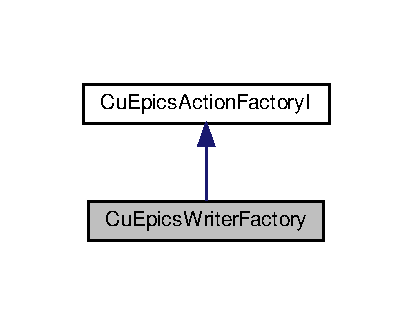
\includegraphics[width=198pt]{classCuEpicsWriterFactory__inherit__graph}
\end{center}
\end{figure}
\subsection*{Public Member Functions}
\begin{DoxyCompactItemize}
\item 
\textbf{ Cu\+Epics\+Writer\+Factory} ()
\item 
void \textbf{ set\+Write\+Value} (const Cu\+Variant \&write\+\_\+val)
\item 
\textbf{ Cu\+Epics\+ActionI} $\ast$ \textbf{ create} (const std\+::string \&s, \textbf{ Cumbia\+Epics} $\ast$ct) const
\item 
\textbf{ Cu\+Epics\+Action\+I\+::\+Type} \textbf{ get\+Type} () const
\begin{DoxyCompactList}\small\item\em Return the type of action that the factory creates. \end{DoxyCompactList}\item 
bool \textbf{ is\+Shareable} () const
\end{DoxyCompactItemize}


\subsection{Constructor \& Destructor Documentation}
\mbox{\label{classCuEpicsWriterFactory_a495f3c5b18c1d90c63fdbb66b1f91458}} 
\index{Cu\+Epics\+Writer\+Factory@{Cu\+Epics\+Writer\+Factory}!Cu\+Epics\+Writer\+Factory@{Cu\+Epics\+Writer\+Factory}}
\index{Cu\+Epics\+Writer\+Factory@{Cu\+Epics\+Writer\+Factory}!Cu\+Epics\+Writer\+Factory@{Cu\+Epics\+Writer\+Factory}}
\subsubsection{Cu\+Epics\+Writer\+Factory()}
{\footnotesize\ttfamily Cu\+Epics\+Writer\+Factory\+::\+Cu\+Epics\+Writer\+Factory (\begin{DoxyParamCaption}{ }\end{DoxyParamCaption})}



\subsection{Member Function Documentation}
\mbox{\label{classCuEpicsWriterFactory_a5244cc75c1b4c4363506811c138d4411}} 
\index{Cu\+Epics\+Writer\+Factory@{Cu\+Epics\+Writer\+Factory}!create@{create}}
\index{create@{create}!Cu\+Epics\+Writer\+Factory@{Cu\+Epics\+Writer\+Factory}}
\subsubsection{create()}
{\footnotesize\ttfamily \textbf{ Cu\+Epics\+ActionI} $\ast$ Cu\+Epics\+Writer\+Factory\+::create (\begin{DoxyParamCaption}\item[{const std\+::string \&}]{s,  }\item[{\textbf{ Cumbia\+Epics} $\ast$}]{ct }\end{DoxyParamCaption}) const\hspace{0.3cm}{\ttfamily [virtual]}}



Implements \textbf{ Cu\+Epics\+Action\+FactoryI} \doxyref{}{p.}{classCuEpicsActionFactoryI_a37e60f748fad19a87626578f8badccf9}.



References Cu\+Put\+::set\+Write\+Value().

\mbox{\label{classCuEpicsWriterFactory_a1c07cf03b37a3648240c5bddae90b669}} 
\index{Cu\+Epics\+Writer\+Factory@{Cu\+Epics\+Writer\+Factory}!get\+Type@{get\+Type}}
\index{get\+Type@{get\+Type}!Cu\+Epics\+Writer\+Factory@{Cu\+Epics\+Writer\+Factory}}
\subsubsection{get\+Type()}
{\footnotesize\ttfamily \textbf{ Cu\+Epics\+Action\+I\+::\+Type} Cu\+Epics\+Writer\+Factory\+::get\+Type (\begin{DoxyParamCaption}{ }\end{DoxyParamCaption}) const\hspace{0.3cm}{\ttfamily [virtual]}}



Return the type of action that the factory creates. 

\begin{DoxyReturn}{Returns}
the type of action that the factory creates 
\end{DoxyReturn}


Implements \textbf{ Cu\+Epics\+Action\+FactoryI} \doxyref{}{p.}{classCuEpicsActionFactoryI_a8fe66bee4e67d957765071ef9d70815f}.



References Cu\+Epics\+Action\+I\+::\+Writer.

\mbox{\label{classCuEpicsWriterFactory_a27bf5c63111b38add7fca0df21490baf}} 
\index{Cu\+Epics\+Writer\+Factory@{Cu\+Epics\+Writer\+Factory}!is\+Shareable@{is\+Shareable}}
\index{is\+Shareable@{is\+Shareable}!Cu\+Epics\+Writer\+Factory@{Cu\+Epics\+Writer\+Factory}}
\subsubsection{is\+Shareable()}
{\footnotesize\ttfamily bool Cu\+Epics\+Writer\+Factory\+::is\+Shareable (\begin{DoxyParamCaption}{ }\end{DoxyParamCaption}) const}

\mbox{\label{classCuEpicsWriterFactory_aac0e5d04e15f2c72e488bbc962cadadc}} 
\index{Cu\+Epics\+Writer\+Factory@{Cu\+Epics\+Writer\+Factory}!set\+Write\+Value@{set\+Write\+Value}}
\index{set\+Write\+Value@{set\+Write\+Value}!Cu\+Epics\+Writer\+Factory@{Cu\+Epics\+Writer\+Factory}}
\subsubsection{set\+Write\+Value()}
{\footnotesize\ttfamily void Cu\+Epics\+Writer\+Factory\+::set\+Write\+Value (\begin{DoxyParamCaption}\item[{const Cu\+Variant \&}]{write\+\_\+val }\end{DoxyParamCaption})}



The documentation for this class was generated from the following files\+:\begin{DoxyCompactItemize}
\item 
\textbf{ cuepactionfactories.\+h}\item 
\textbf{ cuepactionfactories.\+cpp}\end{DoxyCompactItemize}

\section{Cumbia\+Epics Class Reference}
\label{classCumbiaEpics}\index{Cumbia\+Epics@{Cumbia\+Epics}}


Cumbia implementation over the E\+P\+I\+CS control system.  




{\ttfamily \#include $<$cumbiaepics.\+h$>$}



Inheritance diagram for Cumbia\+Epics\+:\nopagebreak
\begin{figure}[H]
\begin{center}
\leavevmode
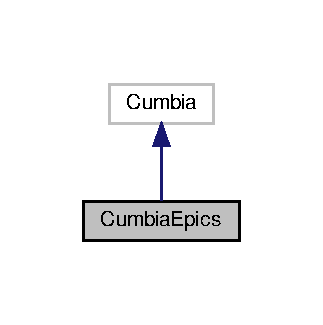
\includegraphics[width=155pt]{classCumbiaEpics__inherit__graph}
\end{center}
\end{figure}
\subsection*{Public Types}
\begin{DoxyCompactItemize}
\item 
enum \textbf{ Type} \{ \textbf{ Cumbia\+Epics\+Type} = Cumbia\+:\+:Cumbia\+User\+Type + 1
 \}
\end{DoxyCompactItemize}
\subsection*{Public Member Functions}
\begin{DoxyCompactItemize}
\item 
\textbf{ Cumbia\+Epics} ()
\item 
\textbf{ Cumbia\+Epics} (Cu\+Thread\+Factory\+ImplI $\ast$tfi, Cu\+Threads\+Event\+Bridge\+Factory\+\_\+I $\ast$teb)
\item 
void \textbf{ set\+Thread\+Factory\+Impl} (Cu\+Thread\+Factory\+ImplI $\ast$tfi)
\item 
void \textbf{ set\+Thread\+Events\+Bridge\+Factory} (Cu\+Threads\+Event\+Bridge\+Factory\+\_\+I $\ast$teb)
\item 
\textbf{ $\sim$\+Cumbia\+Epics} ()
\item 
void \textbf{ add\+Action} (const std\+::string \&source, Cu\+Data\+Listener $\ast$l, const \textbf{ Cu\+Epics\+Action\+FactoryI} \&f)
\item 
void \textbf{ unlink\+Listener} (const std\+::string \&source, \textbf{ Cu\+Epics\+Action\+I\+::\+Type} t, Cu\+Data\+Listener $\ast$l)
\item 
\textbf{ Cu\+Epics\+ActionI} $\ast$ \textbf{ find\+Action} (const std\+::string \&source, \textbf{ Cu\+Epics\+Action\+I\+::\+Type} t) const
\item 
Cu\+Thread\+Factory\+ImplI $\ast$ \textbf{ get\+Thread\+Factory\+Impl} () const
\item 
Cu\+Threads\+Event\+Bridge\+Factory\+\_\+I $\ast$ \textbf{ get\+Thread\+Events\+Bridge\+Factory} () const
\item 
virtual int \textbf{ get\+Type} () const
\end{DoxyCompactItemize}


\subsection{Detailed Description}
Cumbia implementation over the E\+P\+I\+CS control system. 

The {\itshape \doxyref{Cumbia\+Epics}{p.}{classCumbiaEpics}} class is an extension of the {\itshape Cumbia} base one. Its main task is managing the so called {\itshape actions}. An {\itshape action} represents a task associated to an E\+P\+I\+CS {\itshape pv} (called source). Presently, reading from E\+P\+I\+CS is the only action that can be accomplished by {\itshape cumbia-\/epics}. More types of actions are foreseen, such as a writer implementation. {\itshape Cu\+Ep\+ActionI} defines the interface of an action. Operations include adding or removing data listeners, starting and stopping an action, sending and getting data to and from the underlying thread (for example retrieve or change the polling period of a source). {\itshape \doxyref{Cu\+Monitor}{p.}{classCuMonitor}} implements the interface and holds a reference to an activity designed to receive events from {\itshape E\+P\+I\+CS}. 

\subsection{Member Enumeration Documentation}
\mbox{\label{classCumbiaEpics_a81447e0a64b0c0212c109f8c326fdae2}} 
\index{Cumbia\+Epics@{Cumbia\+Epics}!Type@{Type}}
\index{Type@{Type}!Cumbia\+Epics@{Cumbia\+Epics}}
\subsubsection{Type}
{\footnotesize\ttfamily enum \textbf{ Cumbia\+Epics\+::\+Type}}

\begin{DoxyEnumFields}{Enumerator}
\raisebox{\heightof{T}}[0pt][0pt]{\index{Cumbia\+Epics\+Type@{Cumbia\+Epics\+Type}!Cumbia\+Epics@{Cumbia\+Epics}}\index{Cumbia\+Epics@{Cumbia\+Epics}!Cumbia\+Epics\+Type@{Cumbia\+Epics\+Type}}}\mbox{\label{classCumbiaEpics_a81447e0a64b0c0212c109f8c326fdae2adbb35c89e0745de7129176f36c9fec16}} 
Cumbia\+Epics\+Type&\\
\hline

\end{DoxyEnumFields}


\subsection{Constructor \& Destructor Documentation}
\mbox{\label{classCumbiaEpics_a51d6db3f34125d583d474e6f1de51e1c}} 
\index{Cumbia\+Epics@{Cumbia\+Epics}!Cumbia\+Epics@{Cumbia\+Epics}}
\index{Cumbia\+Epics@{Cumbia\+Epics}!Cumbia\+Epics@{Cumbia\+Epics}}
\subsubsection{Cumbia\+Epics()\hspace{0.1cm}{\footnotesize\ttfamily [1/2]}}
{\footnotesize\ttfamily Cumbia\+Epics\+::\+Cumbia\+Epics (\begin{DoxyParamCaption}{ }\end{DoxyParamCaption})}

\mbox{\label{classCumbiaEpics_a9821d489774aa25b128ad4e3a8e08577}} 
\index{Cumbia\+Epics@{Cumbia\+Epics}!Cumbia\+Epics@{Cumbia\+Epics}}
\index{Cumbia\+Epics@{Cumbia\+Epics}!Cumbia\+Epics@{Cumbia\+Epics}}
\subsubsection{Cumbia\+Epics()\hspace{0.1cm}{\footnotesize\ttfamily [2/2]}}
{\footnotesize\ttfamily Cumbia\+Epics\+::\+Cumbia\+Epics (\begin{DoxyParamCaption}\item[{Cu\+Thread\+Factory\+ImplI $\ast$}]{tfi,  }\item[{Cu\+Threads\+Event\+Bridge\+Factory\+\_\+I $\ast$}]{teb }\end{DoxyParamCaption})}

\mbox{\label{classCumbiaEpics_ab1e78162da4328a5fbe0b1cc9de4ca8e}} 
\index{Cumbia\+Epics@{Cumbia\+Epics}!````~Cumbia\+Epics@{$\sim$\+Cumbia\+Epics}}
\index{````~Cumbia\+Epics@{$\sim$\+Cumbia\+Epics}!Cumbia\+Epics@{Cumbia\+Epics}}
\subsubsection{$\sim$\+Cumbia\+Epics()}
{\footnotesize\ttfamily Cumbia\+Epics\+::$\sim$\+Cumbia\+Epics (\begin{DoxyParamCaption}{ }\end{DoxyParamCaption})}



References Cu\+Action\+Factory\+Service\+::\+Cu\+Action\+Factory\+Service\+Type, and Cu\+Action\+Factory\+Service\+::delete\+Actions().



\subsection{Member Function Documentation}
\mbox{\label{classCumbiaEpics_a76a8da66c5f0d7b8984aafc18483a537}} 
\index{Cumbia\+Epics@{Cumbia\+Epics}!add\+Action@{add\+Action}}
\index{add\+Action@{add\+Action}!Cumbia\+Epics@{Cumbia\+Epics}}
\subsubsection{add\+Action()}
{\footnotesize\ttfamily void Cumbia\+Epics\+::add\+Action (\begin{DoxyParamCaption}\item[{const std\+::string \&}]{source,  }\item[{Cu\+Data\+Listener $\ast$}]{l,  }\item[{const \textbf{ Cu\+Epics\+Action\+FactoryI} \&}]{f }\end{DoxyParamCaption})}



References Cu\+Epics\+Action\+I\+::add\+Data\+Listener(), Cu\+Action\+Factory\+Service\+::\+Cu\+Action\+Factory\+Service\+Type, Cu\+Action\+Factory\+Service\+::find\+Action(), Cu\+Epics\+Action\+Factory\+I\+::get\+Type(), Cu\+Action\+Factory\+Service\+::register\+Action(), Cu\+Epics\+World\+::source\+\_\+valid(), and Cu\+Epics\+Action\+I\+::start().

\mbox{\label{classCumbiaEpics_a256da67f6a299263c61d3883b1fe6e28}} 
\index{Cumbia\+Epics@{Cumbia\+Epics}!find\+Action@{find\+Action}}
\index{find\+Action@{find\+Action}!Cumbia\+Epics@{Cumbia\+Epics}}
\subsubsection{find\+Action()}
{\footnotesize\ttfamily \textbf{ Cu\+Epics\+ActionI} $\ast$ Cumbia\+Epics\+::find\+Action (\begin{DoxyParamCaption}\item[{const std\+::string \&}]{source,  }\item[{\textbf{ Cu\+Epics\+Action\+I\+::\+Type}}]{t }\end{DoxyParamCaption}) const}



References Cu\+Action\+Factory\+Service\+::\+Cu\+Action\+Factory\+Service\+Type, and Cu\+Action\+Factory\+Service\+::find\+Action().

\mbox{\label{classCumbiaEpics_aba7f07cee7aced59d7d49cf64fac10d7}} 
\index{Cumbia\+Epics@{Cumbia\+Epics}!get\+Thread\+Events\+Bridge\+Factory@{get\+Thread\+Events\+Bridge\+Factory}}
\index{get\+Thread\+Events\+Bridge\+Factory@{get\+Thread\+Events\+Bridge\+Factory}!Cumbia\+Epics@{Cumbia\+Epics}}
\subsubsection{get\+Thread\+Events\+Bridge\+Factory()}
{\footnotesize\ttfamily Cu\+Threads\+Event\+Bridge\+Factory\+\_\+I $\ast$ Cumbia\+Epics\+::get\+Thread\+Events\+Bridge\+Factory (\begin{DoxyParamCaption}{ }\end{DoxyParamCaption}) const}



Referenced by Cu\+Put\+::start(), and Cu\+Ep\+Configuration\+::start().

\mbox{\label{classCumbiaEpics_a307b03878ba54b2f6014db1bada96c26}} 
\index{Cumbia\+Epics@{Cumbia\+Epics}!get\+Thread\+Factory\+Impl@{get\+Thread\+Factory\+Impl}}
\index{get\+Thread\+Factory\+Impl@{get\+Thread\+Factory\+Impl}!Cumbia\+Epics@{Cumbia\+Epics}}
\subsubsection{get\+Thread\+Factory\+Impl()}
{\footnotesize\ttfamily Cu\+Thread\+Factory\+ImplI $\ast$ Cumbia\+Epics\+::get\+Thread\+Factory\+Impl (\begin{DoxyParamCaption}{ }\end{DoxyParamCaption}) const}



Referenced by Cu\+Put\+::start(), and Cu\+Ep\+Configuration\+::start().

\mbox{\label{classCumbiaEpics_a653cac39c302ebdbad24fead072b8c31}} 
\index{Cumbia\+Epics@{Cumbia\+Epics}!get\+Type@{get\+Type}}
\index{get\+Type@{get\+Type}!Cumbia\+Epics@{Cumbia\+Epics}}
\subsubsection{get\+Type()}
{\footnotesize\ttfamily int Cumbia\+Epics\+::get\+Type (\begin{DoxyParamCaption}{ }\end{DoxyParamCaption}) const\hspace{0.3cm}{\ttfamily [virtual]}}



References Cumbia\+Epics\+Type.

\mbox{\label{classCumbiaEpics_a326e9065965daf1d0449b7aa089daba7}} 
\index{Cumbia\+Epics@{Cumbia\+Epics}!set\+Thread\+Events\+Bridge\+Factory@{set\+Thread\+Events\+Bridge\+Factory}}
\index{set\+Thread\+Events\+Bridge\+Factory@{set\+Thread\+Events\+Bridge\+Factory}!Cumbia\+Epics@{Cumbia\+Epics}}
\subsubsection{set\+Thread\+Events\+Bridge\+Factory()}
{\footnotesize\ttfamily void Cumbia\+Epics\+::set\+Thread\+Events\+Bridge\+Factory (\begin{DoxyParamCaption}\item[{Cu\+Threads\+Event\+Bridge\+Factory\+\_\+I $\ast$}]{teb }\end{DoxyParamCaption})}

\mbox{\label{classCumbiaEpics_ad71f5d1e7f8822a9d99deefdf03eaa50}} 
\index{Cumbia\+Epics@{Cumbia\+Epics}!set\+Thread\+Factory\+Impl@{set\+Thread\+Factory\+Impl}}
\index{set\+Thread\+Factory\+Impl@{set\+Thread\+Factory\+Impl}!Cumbia\+Epics@{Cumbia\+Epics}}
\subsubsection{set\+Thread\+Factory\+Impl()}
{\footnotesize\ttfamily void Cumbia\+Epics\+::set\+Thread\+Factory\+Impl (\begin{DoxyParamCaption}\item[{Cu\+Thread\+Factory\+ImplI $\ast$}]{tfi }\end{DoxyParamCaption})}

\mbox{\label{classCumbiaEpics_af72ad48c477111ae0607995e34bd3ba7}} 
\index{Cumbia\+Epics@{Cumbia\+Epics}!unlink\+Listener@{unlink\+Listener}}
\index{unlink\+Listener@{unlink\+Listener}!Cumbia\+Epics@{Cumbia\+Epics}}
\subsubsection{unlink\+Listener()}
{\footnotesize\ttfamily void Cumbia\+Epics\+::unlink\+Listener (\begin{DoxyParamCaption}\item[{const std\+::string \&}]{source,  }\item[{\textbf{ Cu\+Epics\+Action\+I\+::\+Type}}]{t,  }\item[{Cu\+Data\+Listener $\ast$}]{l }\end{DoxyParamCaption})}



References Cu\+Action\+Factory\+Service\+::\+Cu\+Action\+Factory\+Service\+Type, Cu\+Action\+Factory\+Service\+::find\+Action(), and Cu\+Epics\+Action\+I\+::remove\+Data\+Listener().



The documentation for this class was generated from the following files\+:\begin{DoxyCompactItemize}
\item 
\textbf{ cumbiaepics.\+h}\item 
\textbf{ cumbiaepics.\+cpp}\end{DoxyCompactItemize}

\section{Cu\+Monitor Class Reference}
\label{classCuMonitor}\index{Cu\+Monitor@{Cu\+Monitor}}


{\ttfamily \#include $<$cumonitor.\+h$>$}



Inheritance diagram for Cu\+Monitor\+:\nopagebreak
\begin{figure}[H]
\begin{center}
\leavevmode
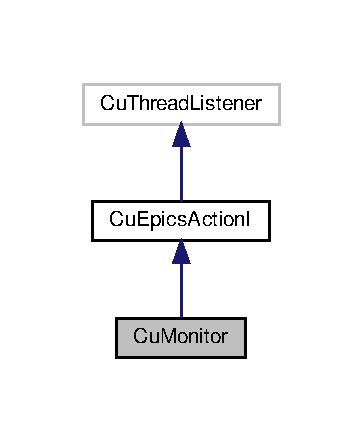
\includegraphics[width=174pt]{classCuMonitor__inherit__graph}
\end{center}
\end{figure}
\subsection*{Public Types}
\begin{DoxyCompactItemize}
\item 
enum \textbf{ Refresh\+Mode} \{ \textbf{ Monitor\+Refresh} = 0, 
\textbf{ Manual}
 \}
\end{DoxyCompactItemize}
\subsection*{Public Member Functions}
\begin{DoxyCompactItemize}
\item 
\textbf{ Cu\+Monitor} (const \textbf{ Ep\+Source} \&src, \textbf{ Cumbia\+Epics} $\ast$ct)
\item 
\textbf{ $\sim$\+Cu\+Monitor} ()
\item 
void \textbf{ on\+Progress} (int step, int total, const Cu\+Data \&data)
\item 
void \textbf{ on\+Result} (const Cu\+Data \&data)
\item 
Cu\+Data \textbf{ get\+Token} () const
\item 
\textbf{ Ep\+Source} \textbf{ get\+Source} () const
\item 
\textbf{ Cu\+Epics\+Action\+I\+::\+Type} \textbf{ get\+Type} () const
\item 
void \textbf{ send\+Data} (const Cu\+Data \&data)
\item 
void \textbf{ get\+Data} (Cu\+Data \&inout) const
\item 
void \textbf{ set\+Refresh\+Mode} (\textbf{ Refresh\+Mode} rm)
\item 
\textbf{ Refresh\+Mode} \textbf{ refresh\+Mode} () const
\item 
void \textbf{ set\+Period} (int millis)
\item 
int \textbf{ period} () const
\item 
void \textbf{ start} ()
\item 
void \textbf{ stop} ()
\item 
void \textbf{ add\+Data\+Listener} (Cu\+Data\+Listener $\ast$l)
\item 
void \textbf{ remove\+Data\+Listener} (Cu\+Data\+Listener $\ast$l)
\item 
size\+\_\+t \textbf{ data\+Listeners\+Count} ()
\end{DoxyCompactItemize}


\subsection{Member Enumeration Documentation}
\mbox{\label{classCuMonitor_a2305dcd4407608a18f4974baadea56bc}} 
\index{Cu\+Monitor@{Cu\+Monitor}!Refresh\+Mode@{Refresh\+Mode}}
\index{Refresh\+Mode@{Refresh\+Mode}!Cu\+Monitor@{Cu\+Monitor}}
\subsubsection{Refresh\+Mode}
{\footnotesize\ttfamily enum \textbf{ Cu\+Monitor\+::\+Refresh\+Mode}}

\begin{DoxyEnumFields}{Enumerator}
\raisebox{\heightof{T}}[0pt][0pt]{\index{Monitor\+Refresh@{Monitor\+Refresh}!Cu\+Monitor@{Cu\+Monitor}}\index{Cu\+Monitor@{Cu\+Monitor}!Monitor\+Refresh@{Monitor\+Refresh}}}\mbox{\label{classCuMonitor_a2305dcd4407608a18f4974baadea56bca4c7227e361f9e94143836c315283fa4e}} 
Monitor\+Refresh&\\
\hline

\raisebox{\heightof{T}}[0pt][0pt]{\index{Manual@{Manual}!Cu\+Monitor@{Cu\+Monitor}}\index{Cu\+Monitor@{Cu\+Monitor}!Manual@{Manual}}}\mbox{\label{classCuMonitor_a2305dcd4407608a18f4974baadea56bca6727f64817e0b5c42ab6710f02ce4715}} 
Manual&\\
\hline

\end{DoxyEnumFields}


\subsection{Constructor \& Destructor Documentation}
\mbox{\label{classCuMonitor_af2cbc5330ba637aca4a34652ca80bbb1}} 
\index{Cu\+Monitor@{Cu\+Monitor}!Cu\+Monitor@{Cu\+Monitor}}
\index{Cu\+Monitor@{Cu\+Monitor}!Cu\+Monitor@{Cu\+Monitor}}
\subsubsection{Cu\+Monitor()}
{\footnotesize\ttfamily Cu\+Monitor\+::\+Cu\+Monitor (\begin{DoxyParamCaption}\item[{const \textbf{ Ep\+Source} \&}]{src,  }\item[{\textbf{ Cumbia\+Epics} $\ast$}]{ct }\end{DoxyParamCaption})}



References Cu\+Monitor\+Private\+::cumbia\+\_\+e, Cu\+Monitor\+Private\+::current\+\_\+activity, Cu\+Monitor\+Private\+::exit, Cu\+Monitor\+Private\+::li, Cu\+Monitor\+Private\+::log, Monitor\+Refresh, Cu\+Monitor\+Private\+::period, Cu\+Monitor\+Private\+::refresh\+\_\+mode, and Cu\+Monitor\+Private\+::tsrc.

\mbox{\label{classCuMonitor_ab2ddd33172dea78aeb2033ee269bc334}} 
\index{Cu\+Monitor@{Cu\+Monitor}!````~Cu\+Monitor@{$\sim$\+Cu\+Monitor}}
\index{````~Cu\+Monitor@{$\sim$\+Cu\+Monitor}!Cu\+Monitor@{Cu\+Monitor}}
\subsubsection{$\sim$\+Cu\+Monitor()}
{\footnotesize\ttfamily Cu\+Monitor\+::$\sim$\+Cu\+Monitor (\begin{DoxyParamCaption}{ }\end{DoxyParamCaption})}



\subsection{Member Function Documentation}
\mbox{\label{classCuMonitor_ac82feb2bd46c4a7b80c8803d8c2716e9}} 
\index{Cu\+Monitor@{Cu\+Monitor}!add\+Data\+Listener@{add\+Data\+Listener}}
\index{add\+Data\+Listener@{add\+Data\+Listener}!Cu\+Monitor@{Cu\+Monitor}}
\subsubsection{add\+Data\+Listener()}
{\footnotesize\ttfamily void Cu\+Monitor\+::add\+Data\+Listener (\begin{DoxyParamCaption}\item[{Cu\+Data\+Listener $\ast$}]{l }\end{DoxyParamCaption})\hspace{0.3cm}{\ttfamily [virtual]}}



Implements \textbf{ Cu\+Epics\+ActionI} \doxyref{}{p.}{classCuEpicsActionI_a8e6c0261f02cb237d612e097fee6dc4a}.



References Cu\+Monitor\+Private\+::listeners.

\mbox{\label{classCuMonitor_a269325e57d5e989c8904ebb12614db43}} 
\index{Cu\+Monitor@{Cu\+Monitor}!data\+Listeners\+Count@{data\+Listeners\+Count}}
\index{data\+Listeners\+Count@{data\+Listeners\+Count}!Cu\+Monitor@{Cu\+Monitor}}
\subsubsection{data\+Listeners\+Count()}
{\footnotesize\ttfamily size\+\_\+t Cu\+Monitor\+::data\+Listeners\+Count (\begin{DoxyParamCaption}{ }\end{DoxyParamCaption})\hspace{0.3cm}{\ttfamily [virtual]}}



Implements \textbf{ Cu\+Epics\+ActionI} \doxyref{}{p.}{classCuEpicsActionI_af7b509410aaee059c3105dfb10b33ee7}.



References Cu\+Monitor\+Private\+::listeners.

\mbox{\label{classCuMonitor_aceebd11ad99f54e64538bd1620377869}} 
\index{Cu\+Monitor@{Cu\+Monitor}!get\+Data@{get\+Data}}
\index{get\+Data@{get\+Data}!Cu\+Monitor@{Cu\+Monitor}}
\subsubsection{get\+Data()}
{\footnotesize\ttfamily void Cu\+Monitor\+::get\+Data (\begin{DoxyParamCaption}\item[{Cu\+Data \&}]{inout }\end{DoxyParamCaption}) const\hspace{0.3cm}{\ttfamily [virtual]}}



Implements \textbf{ Cu\+Epics\+ActionI} \doxyref{}{p.}{classCuEpicsActionI_a063d9436f8a6b84a22a384d06c3996bd}.



References Cu\+Monitor\+Private\+::period, and Cu\+Monitor\+Private\+::refresh\+\_\+mode.

\mbox{\label{classCuMonitor_ae904ab4e124c106476a552cc982e07e6}} 
\index{Cu\+Monitor@{Cu\+Monitor}!get\+Source@{get\+Source}}
\index{get\+Source@{get\+Source}!Cu\+Monitor@{Cu\+Monitor}}
\subsubsection{get\+Source()}
{\footnotesize\ttfamily \textbf{ Ep\+Source} Cu\+Monitor\+::get\+Source (\begin{DoxyParamCaption}{ }\end{DoxyParamCaption}) const\hspace{0.3cm}{\ttfamily [virtual]}}



Implements \textbf{ Cu\+Epics\+ActionI} \doxyref{}{p.}{classCuEpicsActionI_a2c97ba6d9bbd9e98fec51aa92d2becb6}.



References Cu\+Monitor\+Private\+::tsrc.

\mbox{\label{classCuMonitor_a23d9d4d7ae899d0e8fb1914b4af615ad}} 
\index{Cu\+Monitor@{Cu\+Monitor}!get\+Token@{get\+Token}}
\index{get\+Token@{get\+Token}!Cu\+Monitor@{Cu\+Monitor}}
\subsubsection{get\+Token()}
{\footnotesize\ttfamily Cu\+Data Cu\+Monitor\+::get\+Token (\begin{DoxyParamCaption}{ }\end{DoxyParamCaption}) const}



References Ep\+Source\+::get\+Name(), and Cu\+Monitor\+Private\+::tsrc.



Referenced by stop().

\mbox{\label{classCuMonitor_acaffe461ab729a2a0af48a4c77a94292}} 
\index{Cu\+Monitor@{Cu\+Monitor}!get\+Type@{get\+Type}}
\index{get\+Type@{get\+Type}!Cu\+Monitor@{Cu\+Monitor}}
\subsubsection{get\+Type()}
{\footnotesize\ttfamily \textbf{ Cu\+Epics\+Action\+I\+::\+Type} Cu\+Monitor\+::get\+Type (\begin{DoxyParamCaption}{ }\end{DoxyParamCaption}) const\hspace{0.3cm}{\ttfamily [virtual]}}



Implements \textbf{ Cu\+Epics\+ActionI} \doxyref{}{p.}{classCuEpicsActionI_a7386456fda8f1fe44dac1960842b96a6}.



References Cu\+Epics\+Action\+I\+::\+Reader.



Referenced by on\+Result().

\mbox{\label{classCuMonitor_a48187e5840b322239c777a47bff0bb18}} 
\index{Cu\+Monitor@{Cu\+Monitor}!on\+Progress@{on\+Progress}}
\index{on\+Progress@{on\+Progress}!Cu\+Monitor@{Cu\+Monitor}}
\subsubsection{on\+Progress()}
{\footnotesize\ttfamily void Cu\+Monitor\+::on\+Progress (\begin{DoxyParamCaption}\item[{int}]{step,  }\item[{int}]{total,  }\item[{const Cu\+Data \&}]{data }\end{DoxyParamCaption})}

\mbox{\label{classCuMonitor_a69e850603aba7f40f630d109d57ae0a2}} 
\index{Cu\+Monitor@{Cu\+Monitor}!on\+Result@{on\+Result}}
\index{on\+Result@{on\+Result}!Cu\+Monitor@{Cu\+Monitor}}
\subsubsection{on\+Result()}
{\footnotesize\ttfamily void Cu\+Monitor\+::on\+Result (\begin{DoxyParamCaption}\item[{const Cu\+Data \&}]{data }\end{DoxyParamCaption})}



References Cu\+Action\+Factory\+Service\+::\+Cu\+Action\+Factory\+Service\+Type, Cu\+Monitor\+Private\+::cumbia\+\_\+e, Cu\+Monitor\+Private\+::current\+\_\+activity, Cu\+Monitor\+Private\+::exit, Ep\+Source\+::get\+Name(), get\+Type(), Cu\+Monitor\+Private\+::listeners, Cu\+Monitor\+Private\+::tsrc, and Cu\+Action\+Factory\+Service\+::unregister\+Action().

\mbox{\label{classCuMonitor_af8afc0c1b90ed0f4e1866fbb7d690e05}} 
\index{Cu\+Monitor@{Cu\+Monitor}!period@{period}}
\index{period@{period}!Cu\+Monitor@{Cu\+Monitor}}
\subsubsection{period()}
{\footnotesize\ttfamily int Cu\+Monitor\+::period (\begin{DoxyParamCaption}{ }\end{DoxyParamCaption}) const}



References Cu\+Monitor\+Private\+::period.

\mbox{\label{classCuMonitor_a4dc96cd9da274381d93e5f0d373698e2}} 
\index{Cu\+Monitor@{Cu\+Monitor}!refresh\+Mode@{refresh\+Mode}}
\index{refresh\+Mode@{refresh\+Mode}!Cu\+Monitor@{Cu\+Monitor}}
\subsubsection{refresh\+Mode()}
{\footnotesize\ttfamily \textbf{ Cu\+Monitor\+::\+Refresh\+Mode} Cu\+Monitor\+::refresh\+Mode (\begin{DoxyParamCaption}{ }\end{DoxyParamCaption}) const}



References Cu\+Monitor\+Private\+::refresh\+\_\+mode.

\mbox{\label{classCuMonitor_a5b4b77c29cfb45591f4e4a486c8e5000}} 
\index{Cu\+Monitor@{Cu\+Monitor}!remove\+Data\+Listener@{remove\+Data\+Listener}}
\index{remove\+Data\+Listener@{remove\+Data\+Listener}!Cu\+Monitor@{Cu\+Monitor}}
\subsubsection{remove\+Data\+Listener()}
{\footnotesize\ttfamily void Cu\+Monitor\+::remove\+Data\+Listener (\begin{DoxyParamCaption}\item[{Cu\+Data\+Listener $\ast$}]{l }\end{DoxyParamCaption})\hspace{0.3cm}{\ttfamily [virtual]}}



Implements \textbf{ Cu\+Epics\+ActionI} \doxyref{}{p.}{classCuEpicsActionI_a5f5c5045ae8f93ed95794538c495dfdf}.



References Cu\+Monitor\+Private\+::listeners, and stop().

\mbox{\label{classCuMonitor_ad40b612c2d9b8864d92523a40e5e663a}} 
\index{Cu\+Monitor@{Cu\+Monitor}!send\+Data@{send\+Data}}
\index{send\+Data@{send\+Data}!Cu\+Monitor@{Cu\+Monitor}}
\subsubsection{send\+Data()}
{\footnotesize\ttfamily void Cu\+Monitor\+::send\+Data (\begin{DoxyParamCaption}\item[{const Cu\+Data \&}]{data }\end{DoxyParamCaption})\hspace{0.3cm}{\ttfamily [virtual]}}



Implements \textbf{ Cu\+Epics\+ActionI} \doxyref{}{p.}{classCuEpicsActionI_acced5eb52ec2b30b2f21ca30b043d683}.



References Cu\+Monitor\+Activity\+::\+Cu\+Monitor\+Activity\+Type, Cu\+Monitor\+Private\+::current\+\_\+activity, Cu\+Monitor\+Private\+::period, Cu\+Monitor\+Private\+::refresh\+\_\+mode, and set\+Refresh\+Mode().

\mbox{\label{classCuMonitor_a80e523fa66da71cd767f60a39a5a6adb}} 
\index{Cu\+Monitor@{Cu\+Monitor}!set\+Period@{set\+Period}}
\index{set\+Period@{set\+Period}!Cu\+Monitor@{Cu\+Monitor}}
\subsubsection{set\+Period()}
{\footnotesize\ttfamily void Cu\+Monitor\+::set\+Period (\begin{DoxyParamCaption}\item[{int}]{millis }\end{DoxyParamCaption})}



References Cu\+Monitor\+Private\+::period.



Referenced by Cu\+Epics\+Reader\+Factory\+::create().

\mbox{\label{classCuMonitor_a6359ffb94a39fd4126192dc475cf3281}} 
\index{Cu\+Monitor@{Cu\+Monitor}!set\+Refresh\+Mode@{set\+Refresh\+Mode}}
\index{set\+Refresh\+Mode@{set\+Refresh\+Mode}!Cu\+Monitor@{Cu\+Monitor}}
\subsubsection{set\+Refresh\+Mode()}
{\footnotesize\ttfamily void Cu\+Monitor\+::set\+Refresh\+Mode (\begin{DoxyParamCaption}\item[{\textbf{ Cu\+Monitor\+::\+Refresh\+Mode}}]{rm }\end{DoxyParamCaption})}



Referenced by Cu\+Epics\+Reader\+Factory\+::create(), and send\+Data().

\mbox{\label{classCuMonitor_a120832bff1f21fab34cf3a4bcf43af60}} 
\index{Cu\+Monitor@{Cu\+Monitor}!start@{start}}
\index{start@{start}!Cu\+Monitor@{Cu\+Monitor}}
\subsubsection{start()}
{\footnotesize\ttfamily void Cu\+Monitor\+::start (\begin{DoxyParamCaption}{ }\end{DoxyParamCaption})\hspace{0.3cm}{\ttfamily [virtual]}}



Implements \textbf{ Cu\+Epics\+ActionI} \doxyref{}{p.}{classCuEpicsActionI_aa6b252261a7763d5e4266b9a68042cac}.

\mbox{\label{classCuMonitor_a03599f48c24d5f9ba63304a0f03cb144}} 
\index{Cu\+Monitor@{Cu\+Monitor}!stop@{stop}}
\index{stop@{stop}!Cu\+Monitor@{Cu\+Monitor}}
\subsubsection{stop()}
{\footnotesize\ttfamily void Cu\+Monitor\+::stop (\begin{DoxyParamCaption}{ }\end{DoxyParamCaption})\hspace{0.3cm}{\ttfamily [virtual]}}



Implements \textbf{ Cu\+Epics\+ActionI} \doxyref{}{p.}{classCuEpicsActionI_adf2f365700c5cc859929db4495216323}.



References Cu\+Monitor\+Private\+::cumbia\+\_\+e, Cu\+Monitor\+Activity\+::\+Cu\+Monitor\+Activity\+Type, Cu\+Monitor\+Private\+::current\+\_\+activity, Cu\+Monitor\+Private\+::exit, get\+Token(), and Cu\+Monitor\+Private\+::log.



Referenced by remove\+Data\+Listener().



The documentation for this class was generated from the following files\+:\begin{DoxyCompactItemize}
\item 
\textbf{ cumonitor.\+h}\item 
\textbf{ cumonitor.\+cpp}\end{DoxyCompactItemize}

\section{Cu\+Monitor\+Activity Class Reference}
\label{classCuMonitorActivity}\index{Cu\+Monitor\+Activity@{Cu\+Monitor\+Activity}}


{\ttfamily \#include $<$cumonitoractivity.\+h$>$}



Inheritance diagram for Cu\+Monitor\+Activity\+:\nopagebreak
\begin{figure}[H]
\begin{center}
\leavevmode
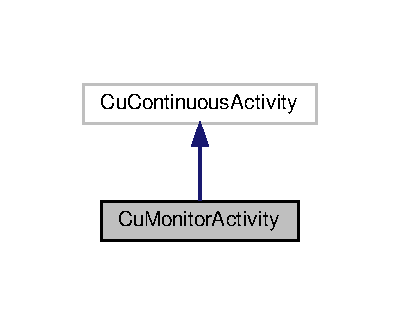
\includegraphics[width=192pt]{classCuMonitorActivity__inherit__graph}
\end{center}
\end{figure}
\subsection*{Public Types}
\begin{DoxyCompactItemize}
\item 
enum \textbf{ Type} \{ \textbf{ Cu\+Monitor\+Activity\+Type} = Cu\+Activity\+:\+:User + 16
 \}
\end{DoxyCompactItemize}
\subsection*{Public Member Functions}
\begin{DoxyCompactItemize}
\item 
\textbf{ Cu\+Monitor\+Activity} (const Cu\+Data \&token, \textbf{ Cu\+Ep\+C\+A\+Service} $\ast$ep\+\_\+s, const Cu\+Variant \&argins=std\+::vector$<$ std\+::string $>$())
\item 
\textbf{ $\sim$\+Cu\+Monitor\+Activity} ()
\item 
void \textbf{ set\+Argins} (const Cu\+Variant \&argins)
\item 
void \textbf{ event\+\_\+handler} (evargs args)
\item 
void \textbf{ connection\+\_\+handler} (connection\+\_\+handler\+\_\+args args)
\item 
void \textbf{ exception\+\_\+handler} (struct exception\+\_\+handler\+\_\+args excargs)
\item 
bool \textbf{ matches} (const Cu\+Data \&token) const
\item 
void \textbf{ event} (Cu\+Activity\+Event $\ast$e)
\item 
int \textbf{ get\+Type} () const
\item 
int \textbf{ repeat} () const
\end{DoxyCompactItemize}
\subsection*{Static Public Member Functions}
\begin{DoxyCompactItemize}
\item 
static void \textbf{ event\+\_\+handler\+\_\+cb} (evargs args)
\item 
static void \textbf{ connection\+\_\+handler\+\_\+cb} (connection\+\_\+handler\+\_\+args args)
\item 
static void \textbf{ exception\+\_\+handler\+\_\+cb} (struct exception\+\_\+handler\+\_\+args excargs)
\end{DoxyCompactItemize}
\subsection*{Protected Member Functions}
\begin{DoxyCompactItemize}
\item 
void \textbf{ init} ()
\item 
void \textbf{ execute} ()
\item 
void \textbf{ on\+Exit} ()
\end{DoxyCompactItemize}


\subsection{Member Enumeration Documentation}
\mbox{\label{classCuMonitorActivity_a9b300629c9bf253981975798e662c1b8}} 
\index{Cu\+Monitor\+Activity@{Cu\+Monitor\+Activity}!Type@{Type}}
\index{Type@{Type}!Cu\+Monitor\+Activity@{Cu\+Monitor\+Activity}}
\subsubsection{Type}
{\footnotesize\ttfamily enum \textbf{ Cu\+Monitor\+Activity\+::\+Type}}

\begin{DoxyEnumFields}{Enumerator}
\raisebox{\heightof{T}}[0pt][0pt]{\index{Cu\+Monitor\+Activity\+Type@{Cu\+Monitor\+Activity\+Type}!Cu\+Monitor\+Activity@{Cu\+Monitor\+Activity}}\index{Cu\+Monitor\+Activity@{Cu\+Monitor\+Activity}!Cu\+Monitor\+Activity\+Type@{Cu\+Monitor\+Activity\+Type}}}\mbox{\label{classCuMonitorActivity_a9b300629c9bf253981975798e662c1b8aba9592e133e9274c45ac7e2efcf9c81e}} 
Cu\+Monitor\+Activity\+Type&\\
\hline

\end{DoxyEnumFields}


\subsection{Constructor \& Destructor Documentation}
\mbox{\label{classCuMonitorActivity_af6604312a7d09913db86fec86d1e4a44}} 
\index{Cu\+Monitor\+Activity@{Cu\+Monitor\+Activity}!Cu\+Monitor\+Activity@{Cu\+Monitor\+Activity}}
\index{Cu\+Monitor\+Activity@{Cu\+Monitor\+Activity}!Cu\+Monitor\+Activity@{Cu\+Monitor\+Activity}}
\subsubsection{Cu\+Monitor\+Activity()}
{\footnotesize\ttfamily Cu\+Monitor\+Activity\+::\+Cu\+Monitor\+Activity (\begin{DoxyParamCaption}\item[{const Cu\+Data \&}]{token,  }\item[{\textbf{ Cu\+Ep\+C\+A\+Service} $\ast$}]{ep\+\_\+s,  }\item[{const Cu\+Variant \&}]{argins = {\ttfamily std\+:\+:vector$<$std\+:\+:string$>$()} }\end{DoxyParamCaption})}



References Cu\+Monitor\+Activity\+Private\+::argins, Cu\+Monitor\+Activity\+Private\+::device\+\_\+srvc, Cu\+Monitor\+Activity\+Private\+::err\+Cnt, Cu\+Monitor\+Activity\+Private\+::exiting, Cu\+Monitor\+Activity\+Private\+::other\+\_\+thread\+\_\+id, and Cu\+Monitor\+Activity\+Private\+::repeat.

\mbox{\label{classCuMonitorActivity_a09d298bf6e31647caa68ed854f42e72b}} 
\index{Cu\+Monitor\+Activity@{Cu\+Monitor\+Activity}!````~Cu\+Monitor\+Activity@{$\sim$\+Cu\+Monitor\+Activity}}
\index{````~Cu\+Monitor\+Activity@{$\sim$\+Cu\+Monitor\+Activity}!Cu\+Monitor\+Activity@{Cu\+Monitor\+Activity}}
\subsubsection{$\sim$\+Cu\+Monitor\+Activity()}
{\footnotesize\ttfamily Cu\+Monitor\+Activity\+::$\sim$\+Cu\+Monitor\+Activity (\begin{DoxyParamCaption}{ }\end{DoxyParamCaption})}



\subsection{Member Function Documentation}
\mbox{\label{classCuMonitorActivity_a71f2bc9f31906dc44b53a31c7a625661}} 
\index{Cu\+Monitor\+Activity@{Cu\+Monitor\+Activity}!connection\+\_\+handler@{connection\+\_\+handler}}
\index{connection\+\_\+handler@{connection\+\_\+handler}!Cu\+Monitor\+Activity@{Cu\+Monitor\+Activity}}
\subsubsection{connection\+\_\+handler()}
{\footnotesize\ttfamily void Cu\+Monitor\+Activity\+::connection\+\_\+handler (\begin{DoxyParamCaption}\item[{connection\+\_\+handler\+\_\+args}]{args }\end{DoxyParamCaption})}



References Cu\+P\+V\+::ch\+\_\+id, Cu\+P\+V\+::dbf\+Type, Cu\+P\+V\+::dbr\+Type, enum\+As\+Nr, event\+\_\+handler\+\_\+cb(), Cu\+P\+V\+::n\+Elems, Cu\+P\+V\+::once\+Connected, Cu\+P\+V\+::req\+Elems, and Cu\+P\+V\+::status.



Referenced by connection\+\_\+handler\+\_\+cb().

\mbox{\label{classCuMonitorActivity_a3431eb975b72609d04f682ff5f2152fb}} 
\index{Cu\+Monitor\+Activity@{Cu\+Monitor\+Activity}!connection\+\_\+handler\+\_\+cb@{connection\+\_\+handler\+\_\+cb}}
\index{connection\+\_\+handler\+\_\+cb@{connection\+\_\+handler\+\_\+cb}!Cu\+Monitor\+Activity@{Cu\+Monitor\+Activity}}
\subsubsection{connection\+\_\+handler\+\_\+cb()}
{\footnotesize\ttfamily void Cu\+Monitor\+Activity\+::connection\+\_\+handler\+\_\+cb (\begin{DoxyParamCaption}\item[{connection\+\_\+handler\+\_\+args}]{args }\end{DoxyParamCaption})\hspace{0.3cm}{\ttfamily [static]}}



References connection\+\_\+handler(), and Cu\+P\+V\+::monitor\+\_\+activity.



Referenced by init().

\mbox{\label{classCuMonitorActivity_a03d32b6b8dfc336985756910b166febc}} 
\index{Cu\+Monitor\+Activity@{Cu\+Monitor\+Activity}!event@{event}}
\index{event@{event}!Cu\+Monitor\+Activity@{Cu\+Monitor\+Activity}}
\subsubsection{event()}
{\footnotesize\ttfamily void Cu\+Monitor\+Activity\+::event (\begin{DoxyParamCaption}\item[{Cu\+Activity\+Event $\ast$}]{e }\end{DoxyParamCaption})}



References Cu\+Monitor\+Activity\+Private\+::my\+\_\+thread\+\_\+id.

\mbox{\label{classCuMonitorActivity_a3c754227c64d922e1f3b0e0a9287c1f4}} 
\index{Cu\+Monitor\+Activity@{Cu\+Monitor\+Activity}!event\+\_\+handler@{event\+\_\+handler}}
\index{event\+\_\+handler@{event\+\_\+handler}!Cu\+Monitor\+Activity@{Cu\+Monitor\+Activity}}
\subsubsection{event\+\_\+handler()}
{\footnotesize\ttfamily void Cu\+Monitor\+Activity\+::event\+\_\+handler (\begin{DoxyParamCaption}\item[{evargs}]{args }\end{DoxyParamCaption})}



References Cu\+P\+V\+::dbr\+Type, Cu\+Epics\+World\+::error(), Cu\+Epics\+World\+::extract\+Data(), Cu\+Epics\+World\+::fill\+Thread\+Info(), Cu\+Epics\+World\+::get\+Last\+Message(), Cu\+P\+V\+::name, Cu\+P\+V\+::n\+Elems, Cu\+P\+V\+::status, and Cu\+P\+V\+::value.



Referenced by event\+\_\+handler\+\_\+cb().

\mbox{\label{classCuMonitorActivity_a72f2cce818ca383a5d0eba77baa14838}} 
\index{Cu\+Monitor\+Activity@{Cu\+Monitor\+Activity}!event\+\_\+handler\+\_\+cb@{event\+\_\+handler\+\_\+cb}}
\index{event\+\_\+handler\+\_\+cb@{event\+\_\+handler\+\_\+cb}!Cu\+Monitor\+Activity@{Cu\+Monitor\+Activity}}
\subsubsection{event\+\_\+handler\+\_\+cb()}
{\footnotesize\ttfamily void Cu\+Monitor\+Activity\+::event\+\_\+handler\+\_\+cb (\begin{DoxyParamCaption}\item[{evargs}]{args }\end{DoxyParamCaption})\hspace{0.3cm}{\ttfamily [static]}}



References event\+\_\+handler(), and Cu\+P\+V\+::monitor\+\_\+activity.



Referenced by connection\+\_\+handler().

\mbox{\label{classCuMonitorActivity_a2a673ca8237588df5d6722ec325bd466}} 
\index{Cu\+Monitor\+Activity@{Cu\+Monitor\+Activity}!exception\+\_\+handler@{exception\+\_\+handler}}
\index{exception\+\_\+handler@{exception\+\_\+handler}!Cu\+Monitor\+Activity@{Cu\+Monitor\+Activity}}
\subsubsection{exception\+\_\+handler()}
{\footnotesize\ttfamily void Cu\+Monitor\+Activity\+::exception\+\_\+handler (\begin{DoxyParamCaption}\item[{struct exception\+\_\+handler\+\_\+args}]{excargs }\end{DoxyParamCaption})}



References Cu\+Epics\+World\+::extract\+Exception().



Referenced by exception\+\_\+handler\+\_\+cb().

\mbox{\label{classCuMonitorActivity_afc62496d0b4171ce99e073082e9b64da}} 
\index{Cu\+Monitor\+Activity@{Cu\+Monitor\+Activity}!exception\+\_\+handler\+\_\+cb@{exception\+\_\+handler\+\_\+cb}}
\index{exception\+\_\+handler\+\_\+cb@{exception\+\_\+handler\+\_\+cb}!Cu\+Monitor\+Activity@{Cu\+Monitor\+Activity}}
\subsubsection{exception\+\_\+handler\+\_\+cb()}
{\footnotesize\ttfamily void Cu\+Monitor\+Activity\+::exception\+\_\+handler\+\_\+cb (\begin{DoxyParamCaption}\item[{struct exception\+\_\+handler\+\_\+args}]{excargs }\end{DoxyParamCaption})\hspace{0.3cm}{\ttfamily [static]}}



References exception\+\_\+handler().



Referenced by init().

\mbox{\label{classCuMonitorActivity_aa639f58d03ad3b91cea5ab9b4f5319ee}} 
\index{Cu\+Monitor\+Activity@{Cu\+Monitor\+Activity}!execute@{execute}}
\index{execute@{execute}!Cu\+Monitor\+Activity@{Cu\+Monitor\+Activity}}
\subsubsection{execute()}
{\footnotesize\ttfamily void Cu\+Monitor\+Activity\+::execute (\begin{DoxyParamCaption}{ }\end{DoxyParamCaption})\hspace{0.3cm}{\ttfamily [protected]}}



References Cu\+Monitor\+Activity\+Private\+::my\+\_\+thread\+\_\+id.

\mbox{\label{classCuMonitorActivity_a7bcf41b05af2c5d047314a028e1dbdd7}} 
\index{Cu\+Monitor\+Activity@{Cu\+Monitor\+Activity}!get\+Type@{get\+Type}}
\index{get\+Type@{get\+Type}!Cu\+Monitor\+Activity@{Cu\+Monitor\+Activity}}
\subsubsection{get\+Type()}
{\footnotesize\ttfamily int Cu\+Monitor\+Activity\+::get\+Type (\begin{DoxyParamCaption}{ }\end{DoxyParamCaption}) const}



References Cu\+Monitor\+Activity\+Type.

\mbox{\label{classCuMonitorActivity_ace0cee769df1f3beda7b21b51e51aa2e}} 
\index{Cu\+Monitor\+Activity@{Cu\+Monitor\+Activity}!init@{init}}
\index{init@{init}!Cu\+Monitor\+Activity@{Cu\+Monitor\+Activity}}
\subsubsection{init()}
{\footnotesize\ttfamily void Cu\+Monitor\+Activity\+::init (\begin{DoxyParamCaption}{ }\end{DoxyParamCaption})\hspace{0.3cm}{\ttfamily [protected]}}



References ca\+Timeout, connection\+\_\+handler\+\_\+cb(), create\+\_\+pvs(), D\+E\+F\+A\+U\+L\+T\+\_\+\+C\+A\+\_\+\+T\+I\+M\+E\+O\+UT, exception\+\_\+handler\+\_\+cb(), Cu\+P\+V\+::monitor\+\_\+activity, Cu\+Monitor\+Activity\+Private\+::my\+\_\+thread\+\_\+id, Cu\+P\+V\+::once\+Connected, Cu\+Monitor\+Activity\+Private\+::other\+\_\+thread\+\_\+id, and Cu\+Monitor\+Activity\+Private\+::repeat.

\mbox{\label{classCuMonitorActivity_a6ba89bf4cdc89f9f6da06cdd51a7dd35}} 
\index{Cu\+Monitor\+Activity@{Cu\+Monitor\+Activity}!matches@{matches}}
\index{matches@{matches}!Cu\+Monitor\+Activity@{Cu\+Monitor\+Activity}}
\subsubsection{matches()}
{\footnotesize\ttfamily bool Cu\+Monitor\+Activity\+::matches (\begin{DoxyParamCaption}\item[{const Cu\+Data \&}]{token }\end{DoxyParamCaption}) const}

\mbox{\label{classCuMonitorActivity_a5a8aedf1f0e6ded9414b3757963f7776}} 
\index{Cu\+Monitor\+Activity@{Cu\+Monitor\+Activity}!on\+Exit@{on\+Exit}}
\index{on\+Exit@{on\+Exit}!Cu\+Monitor\+Activity@{Cu\+Monitor\+Activity}}
\subsubsection{on\+Exit()}
{\footnotesize\ttfamily void Cu\+Monitor\+Activity\+::on\+Exit (\begin{DoxyParamCaption}{ }\end{DoxyParamCaption})\hspace{0.3cm}{\ttfamily [protected]}}



References Cu\+Monitor\+Activity\+Private\+::exiting, Cu\+Epics\+World\+::fill\+Thread\+Info(), and Cu\+Monitor\+Activity\+Private\+::my\+\_\+thread\+\_\+id.

\mbox{\label{classCuMonitorActivity_aa39a0c8aa57dcd927559e151854b89be}} 
\index{Cu\+Monitor\+Activity@{Cu\+Monitor\+Activity}!repeat@{repeat}}
\index{repeat@{repeat}!Cu\+Monitor\+Activity@{Cu\+Monitor\+Activity}}
\subsubsection{repeat()}
{\footnotesize\ttfamily int Cu\+Monitor\+Activity\+::repeat (\begin{DoxyParamCaption}{ }\end{DoxyParamCaption}) const}



References Cu\+Monitor\+Activity\+Private\+::my\+\_\+thread\+\_\+id, and Cu\+Monitor\+Activity\+Private\+::repeat.

\mbox{\label{classCuMonitorActivity_a95f83be4a0bb5b48e2ed58660fab6c75}} 
\index{Cu\+Monitor\+Activity@{Cu\+Monitor\+Activity}!set\+Argins@{set\+Argins}}
\index{set\+Argins@{set\+Argins}!Cu\+Monitor\+Activity@{Cu\+Monitor\+Activity}}
\subsubsection{set\+Argins()}
{\footnotesize\ttfamily void Cu\+Monitor\+Activity\+::set\+Argins (\begin{DoxyParamCaption}\item[{const Cu\+Variant \&}]{argins }\end{DoxyParamCaption})}



References Cu\+Monitor\+Activity\+Private\+::argins.



The documentation for this class was generated from the following files\+:\begin{DoxyCompactItemize}
\item 
\textbf{ cumonitoractivity.\+h}\item 
\textbf{ cumonitoractivity.\+cpp}\end{DoxyCompactItemize}

\section{Cu\+Monitor\+Activity\+Private Class Reference}
\label{classCuMonitorActivityPrivate}\index{Cu\+Monitor\+Activity\+Private@{Cu\+Monitor\+Activity\+Private}}
\subsection*{Public Attributes}
\begin{DoxyCompactItemize}
\item 
\textbf{ Cu\+Ep\+C\+A\+Service} $\ast$ \textbf{ device\+\_\+srvc}
\item 
int \textbf{ repeat}
\item 
int \textbf{ err\+Cnt}
\item 
std\+::string \textbf{ message}
\item 
pthread\+\_\+t \textbf{ my\+\_\+thread\+\_\+id}
\item 
pthread\+\_\+t \textbf{ other\+\_\+thread\+\_\+id}
\item 
Cu\+Variant \textbf{ argins}
\item 
Cu\+Data \textbf{ point\+\_\+info}
\item 
bool \textbf{ exiting}
\end{DoxyCompactItemize}


\subsection{Member Data Documentation}
\mbox{\label{classCuMonitorActivityPrivate_aad65696f71e3a49aef9545adfbe0e7a7}} 
\index{Cu\+Monitor\+Activity\+Private@{Cu\+Monitor\+Activity\+Private}!argins@{argins}}
\index{argins@{argins}!Cu\+Monitor\+Activity\+Private@{Cu\+Monitor\+Activity\+Private}}
\subsubsection{argins}
{\footnotesize\ttfamily Cu\+Variant Cu\+Monitor\+Activity\+Private\+::argins}



Referenced by Cu\+Monitor\+Activity\+::\+Cu\+Monitor\+Activity(), and Cu\+Monitor\+Activity\+::set\+Argins().

\mbox{\label{classCuMonitorActivityPrivate_a8670ac07cd29a34c24f974d27fc34802}} 
\index{Cu\+Monitor\+Activity\+Private@{Cu\+Monitor\+Activity\+Private}!device\+\_\+srvc@{device\+\_\+srvc}}
\index{device\+\_\+srvc@{device\+\_\+srvc}!Cu\+Monitor\+Activity\+Private@{Cu\+Monitor\+Activity\+Private}}
\subsubsection{device\+\_\+srvc}
{\footnotesize\ttfamily \textbf{ Cu\+Ep\+C\+A\+Service}$\ast$ Cu\+Monitor\+Activity\+Private\+::device\+\_\+srvc}



Referenced by Cu\+Monitor\+Activity\+::\+Cu\+Monitor\+Activity().

\mbox{\label{classCuMonitorActivityPrivate_aee1880a845a07056c461f2d7da55884d}} 
\index{Cu\+Monitor\+Activity\+Private@{Cu\+Monitor\+Activity\+Private}!err\+Cnt@{err\+Cnt}}
\index{err\+Cnt@{err\+Cnt}!Cu\+Monitor\+Activity\+Private@{Cu\+Monitor\+Activity\+Private}}
\subsubsection{err\+Cnt}
{\footnotesize\ttfamily int Cu\+Monitor\+Activity\+Private\+::err\+Cnt}



Referenced by Cu\+Monitor\+Activity\+::\+Cu\+Monitor\+Activity().

\mbox{\label{classCuMonitorActivityPrivate_acf6a9a415cc4959e12b4fa1c8375e6b1}} 
\index{Cu\+Monitor\+Activity\+Private@{Cu\+Monitor\+Activity\+Private}!exiting@{exiting}}
\index{exiting@{exiting}!Cu\+Monitor\+Activity\+Private@{Cu\+Monitor\+Activity\+Private}}
\subsubsection{exiting}
{\footnotesize\ttfamily bool Cu\+Monitor\+Activity\+Private\+::exiting}



Referenced by Cu\+Monitor\+Activity\+::\+Cu\+Monitor\+Activity(), and Cu\+Monitor\+Activity\+::on\+Exit().

\mbox{\label{classCuMonitorActivityPrivate_a11da2a275e707ce31a4007dae78eb446}} 
\index{Cu\+Monitor\+Activity\+Private@{Cu\+Monitor\+Activity\+Private}!message@{message}}
\index{message@{message}!Cu\+Monitor\+Activity\+Private@{Cu\+Monitor\+Activity\+Private}}
\subsubsection{message}
{\footnotesize\ttfamily std\+::string Cu\+Monitor\+Activity\+Private\+::message}

\mbox{\label{classCuMonitorActivityPrivate_aea3c151af6edead42f59e5a26169c97b}} 
\index{Cu\+Monitor\+Activity\+Private@{Cu\+Monitor\+Activity\+Private}!my\+\_\+thread\+\_\+id@{my\+\_\+thread\+\_\+id}}
\index{my\+\_\+thread\+\_\+id@{my\+\_\+thread\+\_\+id}!Cu\+Monitor\+Activity\+Private@{Cu\+Monitor\+Activity\+Private}}
\subsubsection{my\+\_\+thread\+\_\+id}
{\footnotesize\ttfamily pthread\+\_\+t Cu\+Monitor\+Activity\+Private\+::my\+\_\+thread\+\_\+id}



Referenced by Cu\+Monitor\+Activity\+::event(), Cu\+Monitor\+Activity\+::execute(), Cu\+Monitor\+Activity\+::init(), Cu\+Monitor\+Activity\+::on\+Exit(), and Cu\+Monitor\+Activity\+::repeat().

\mbox{\label{classCuMonitorActivityPrivate_ad8d937086afaccbb9b686ffeea9969a5}} 
\index{Cu\+Monitor\+Activity\+Private@{Cu\+Monitor\+Activity\+Private}!other\+\_\+thread\+\_\+id@{other\+\_\+thread\+\_\+id}}
\index{other\+\_\+thread\+\_\+id@{other\+\_\+thread\+\_\+id}!Cu\+Monitor\+Activity\+Private@{Cu\+Monitor\+Activity\+Private}}
\subsubsection{other\+\_\+thread\+\_\+id}
{\footnotesize\ttfamily pthread\+\_\+t Cu\+Monitor\+Activity\+Private\+::other\+\_\+thread\+\_\+id}



Referenced by Cu\+Monitor\+Activity\+::\+Cu\+Monitor\+Activity(), and Cu\+Monitor\+Activity\+::init().

\mbox{\label{classCuMonitorActivityPrivate_aa23d8c915a8d8d9dd39c0ee71f2ac2a5}} 
\index{Cu\+Monitor\+Activity\+Private@{Cu\+Monitor\+Activity\+Private}!point\+\_\+info@{point\+\_\+info}}
\index{point\+\_\+info@{point\+\_\+info}!Cu\+Monitor\+Activity\+Private@{Cu\+Monitor\+Activity\+Private}}
\subsubsection{point\+\_\+info}
{\footnotesize\ttfamily Cu\+Data Cu\+Monitor\+Activity\+Private\+::point\+\_\+info}

\mbox{\label{classCuMonitorActivityPrivate_a0779e4f5ee7ef2aa56d5a1a9bc020f56}} 
\index{Cu\+Monitor\+Activity\+Private@{Cu\+Monitor\+Activity\+Private}!repeat@{repeat}}
\index{repeat@{repeat}!Cu\+Monitor\+Activity\+Private@{Cu\+Monitor\+Activity\+Private}}
\subsubsection{repeat}
{\footnotesize\ttfamily int Cu\+Monitor\+Activity\+Private\+::repeat}



Referenced by Cu\+Monitor\+Activity\+::\+Cu\+Monitor\+Activity(), Cu\+Monitor\+Activity\+::init(), and Cu\+Monitor\+Activity\+::repeat().



The documentation for this class was generated from the following file\+:\begin{DoxyCompactItemize}
\item 
\textbf{ cumonitoractivity.\+cpp}\end{DoxyCompactItemize}

\section{Cu\+Monitor\+Private Class Reference}
\label{classCuMonitorPrivate}\index{Cu\+Monitor\+Private@{Cu\+Monitor\+Private}}
\subsection*{Public Attributes}
\begin{DoxyCompactItemize}
\item 
std\+::list$<$ Cu\+Data\+Listener $\ast$ $>$ \textbf{ listeners}
\item 
\textbf{ Ep\+Source} \textbf{ tsrc}
\item 
\textbf{ Cumbia\+Epics} $\ast$ \textbf{ cumbia\+\_\+e}
\item 
Cu\+Activity $\ast$ \textbf{ current\+\_\+activity}
\item 
bool \textbf{ exit}
\item 
Cu\+Con\+Log\+Impl \textbf{ li}
\item 
Cu\+Log \textbf{ log}
\item 
int \textbf{ period}
\item 
\textbf{ Cu\+Monitor\+::\+Refresh\+Mode} \textbf{ refresh\+\_\+mode}
\end{DoxyCompactItemize}


\subsection{Member Data Documentation}
\mbox{\label{classCuMonitorPrivate_a246616adf3f6d59bc9d9f017aa3a7dec}} 
\index{Cu\+Monitor\+Private@{Cu\+Monitor\+Private}!cumbia\+\_\+e@{cumbia\+\_\+e}}
\index{cumbia\+\_\+e@{cumbia\+\_\+e}!Cu\+Monitor\+Private@{Cu\+Monitor\+Private}}
\subsubsection{cumbia\+\_\+e}
{\footnotesize\ttfamily \textbf{ Cumbia\+Epics}$\ast$ Cu\+Monitor\+Private\+::cumbia\+\_\+e}



Referenced by Cu\+Monitor\+::\+Cu\+Monitor(), Cu\+Monitor\+::on\+Result(), and Cu\+Monitor\+::stop().

\mbox{\label{classCuMonitorPrivate_a8fffc9675988d2e5abab9111c0d486f1}} 
\index{Cu\+Monitor\+Private@{Cu\+Monitor\+Private}!current\+\_\+activity@{current\+\_\+activity}}
\index{current\+\_\+activity@{current\+\_\+activity}!Cu\+Monitor\+Private@{Cu\+Monitor\+Private}}
\subsubsection{current\+\_\+activity}
{\footnotesize\ttfamily Cu\+Activity$\ast$ Cu\+Monitor\+Private\+::current\+\_\+activity}



Referenced by Cu\+Monitor\+::\+Cu\+Monitor(), Cu\+Monitor\+::on\+Result(), Cu\+Monitor\+::send\+Data(), and Cu\+Monitor\+::stop().

\mbox{\label{classCuMonitorPrivate_a6af7851eb453387b319956e83010b579}} 
\index{Cu\+Monitor\+Private@{Cu\+Monitor\+Private}!exit@{exit}}
\index{exit@{exit}!Cu\+Monitor\+Private@{Cu\+Monitor\+Private}}
\subsubsection{exit}
{\footnotesize\ttfamily bool Cu\+Monitor\+Private\+::exit}



Referenced by Cu\+Monitor\+::\+Cu\+Monitor(), Cu\+Monitor\+::on\+Result(), and Cu\+Monitor\+::stop().

\mbox{\label{classCuMonitorPrivate_aeeddf8d712a455f074ff49819c62589f}} 
\index{Cu\+Monitor\+Private@{Cu\+Monitor\+Private}!li@{li}}
\index{li@{li}!Cu\+Monitor\+Private@{Cu\+Monitor\+Private}}
\subsubsection{li}
{\footnotesize\ttfamily Cu\+Con\+Log\+Impl Cu\+Monitor\+Private\+::li}



Referenced by Cu\+Monitor\+::\+Cu\+Monitor().

\mbox{\label{classCuMonitorPrivate_abb87f9db3a9dea818e42dfa9fe4c4462}} 
\index{Cu\+Monitor\+Private@{Cu\+Monitor\+Private}!listeners@{listeners}}
\index{listeners@{listeners}!Cu\+Monitor\+Private@{Cu\+Monitor\+Private}}
\subsubsection{listeners}
{\footnotesize\ttfamily std\+::list$<$Cu\+Data\+Listener $\ast$$>$ Cu\+Monitor\+Private\+::listeners}



Referenced by Cu\+Monitor\+::add\+Data\+Listener(), Cu\+Monitor\+::data\+Listeners\+Count(), Cu\+Monitor\+::on\+Result(), and Cu\+Monitor\+::remove\+Data\+Listener().

\mbox{\label{classCuMonitorPrivate_a655f97ece1a8399381618a2b66c6ce0b}} 
\index{Cu\+Monitor\+Private@{Cu\+Monitor\+Private}!log@{log}}
\index{log@{log}!Cu\+Monitor\+Private@{Cu\+Monitor\+Private}}
\subsubsection{log}
{\footnotesize\ttfamily Cu\+Log Cu\+Monitor\+Private\+::log}



Referenced by Cu\+Monitor\+::\+Cu\+Monitor(), and Cu\+Monitor\+::stop().

\mbox{\label{classCuMonitorPrivate_aed81d4c836ac777391117449646d12c7}} 
\index{Cu\+Monitor\+Private@{Cu\+Monitor\+Private}!period@{period}}
\index{period@{period}!Cu\+Monitor\+Private@{Cu\+Monitor\+Private}}
\subsubsection{period}
{\footnotesize\ttfamily int Cu\+Monitor\+Private\+::period}



Referenced by Cu\+Monitor\+::\+Cu\+Monitor(), Cu\+Monitor\+::get\+Data(), Cu\+Monitor\+::period(), Cu\+Monitor\+::send\+Data(), and Cu\+Monitor\+::set\+Period().

\mbox{\label{classCuMonitorPrivate_a42138e7a75d47eb39cf4560d76d90c91}} 
\index{Cu\+Monitor\+Private@{Cu\+Monitor\+Private}!refresh\+\_\+mode@{refresh\+\_\+mode}}
\index{refresh\+\_\+mode@{refresh\+\_\+mode}!Cu\+Monitor\+Private@{Cu\+Monitor\+Private}}
\subsubsection{refresh\+\_\+mode}
{\footnotesize\ttfamily \textbf{ Cu\+Monitor\+::\+Refresh\+Mode} Cu\+Monitor\+Private\+::refresh\+\_\+mode}



Referenced by Cu\+Monitor\+::\+Cu\+Monitor(), Cu\+Monitor\+::get\+Data(), Cu\+Monitor\+::refresh\+Mode(), and Cu\+Monitor\+::send\+Data().

\mbox{\label{classCuMonitorPrivate_a2a10c4044b8f1678b92e53b5d139c2d6}} 
\index{Cu\+Monitor\+Private@{Cu\+Monitor\+Private}!tsrc@{tsrc}}
\index{tsrc@{tsrc}!Cu\+Monitor\+Private@{Cu\+Monitor\+Private}}
\subsubsection{tsrc}
{\footnotesize\ttfamily \textbf{ Ep\+Source} Cu\+Monitor\+Private\+::tsrc}



Referenced by Cu\+Monitor\+::\+Cu\+Monitor(), Cu\+Monitor\+::get\+Source(), Cu\+Monitor\+::get\+Token(), and Cu\+Monitor\+::on\+Result().



The documentation for this class was generated from the following file\+:\begin{DoxyCompactItemize}
\item 
\textbf{ cumonitor.\+cpp}\end{DoxyCompactItemize}

\section{Cu\+Put Class Reference}
\label{classCuPut}\index{Cu\+Put@{Cu\+Put}}


{\ttfamily \#include $<$cuput.\+h$>$}



Inheritance diagram for Cu\+Put\+:\nopagebreak
\begin{figure}[H]
\begin{center}
\leavevmode
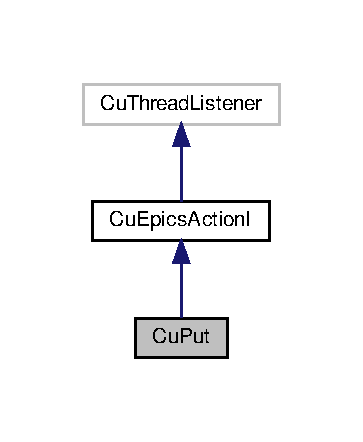
\includegraphics[width=174pt]{classCuPut__inherit__graph}
\end{center}
\end{figure}
\subsection*{Public Member Functions}
\begin{DoxyCompactItemize}
\item 
\textbf{ Cu\+Put} (const \textbf{ Ep\+Source} \&src, \textbf{ Cumbia\+Epics} $\ast$ct)
\item 
virtual \textbf{ $\sim$\+Cu\+Put} ()
\item 
void \textbf{ set\+Write\+Value} (const Cu\+Variant \&wval)
\item 
void \textbf{ on\+Progress} (int step, int total, const Cu\+Data \&data)
\item 
void \textbf{ on\+Result} (const Cu\+Data \&data)
\item 
Cu\+Data \textbf{ get\+Token} () const
\item 
\textbf{ Ep\+Source} \textbf{ get\+Source} () const
\item 
\textbf{ Type} \textbf{ get\+Type} () const
\item 
void \textbf{ add\+Data\+Listener} (Cu\+Data\+Listener $\ast$l)
\item 
void \textbf{ remove\+Data\+Listener} (Cu\+Data\+Listener $\ast$l)
\item 
size\+\_\+t \textbf{ data\+Listeners\+Count} ()
\item 
void \textbf{ start} ()
\item 
void \textbf{ stop} ()
\item 
void \textbf{ send\+Data} (const Cu\+Data \&data)
\item 
void \textbf{ get\+Data} (Cu\+Data \&d\+\_\+inout) const
\end{DoxyCompactItemize}
\subsection*{Additional Inherited Members}


\subsection{Constructor \& Destructor Documentation}
\mbox{\label{classCuPut_a5aca2baf30558b8a30a5ba19d99207d3}} 
\index{Cu\+Put@{Cu\+Put}!Cu\+Put@{Cu\+Put}}
\index{Cu\+Put@{Cu\+Put}!Cu\+Put@{Cu\+Put}}
\subsubsection{Cu\+Put()}
{\footnotesize\ttfamily Cu\+Put\+::\+Cu\+Put (\begin{DoxyParamCaption}\item[{const \textbf{ Ep\+Source} \&}]{src,  }\item[{\textbf{ Cumbia\+Epics} $\ast$}]{ct }\end{DoxyParamCaption})}



References Cu\+T\+Writer\+Private\+::cumbia\+\_\+t, Cu\+T\+Writer\+Private\+::exit, Cu\+T\+Writer\+Private\+::li, Cu\+T\+Writer\+Private\+::log, and Cu\+T\+Writer\+Private\+::tsrc.

\mbox{\label{classCuPut_a62203bda48a30fa4a8a966a4d039ba7b}} 
\index{Cu\+Put@{Cu\+Put}!````~Cu\+Put@{$\sim$\+Cu\+Put}}
\index{````~Cu\+Put@{$\sim$\+Cu\+Put}!Cu\+Put@{Cu\+Put}}
\subsubsection{$\sim$\+Cu\+Put()}
{\footnotesize\ttfamily Cu\+Put\+::$\sim$\+Cu\+Put (\begin{DoxyParamCaption}{ }\end{DoxyParamCaption})\hspace{0.3cm}{\ttfamily [virtual]}}



\subsection{Member Function Documentation}
\mbox{\label{classCuPut_a304735be4bbef6c03d30862dd69e9213}} 
\index{Cu\+Put@{Cu\+Put}!add\+Data\+Listener@{add\+Data\+Listener}}
\index{add\+Data\+Listener@{add\+Data\+Listener}!Cu\+Put@{Cu\+Put}}
\subsubsection{add\+Data\+Listener()}
{\footnotesize\ttfamily void Cu\+Put\+::add\+Data\+Listener (\begin{DoxyParamCaption}\item[{Cu\+Data\+Listener $\ast$}]{l }\end{DoxyParamCaption})\hspace{0.3cm}{\ttfamily [virtual]}}



Implements \textbf{ Cu\+Epics\+ActionI} \doxyref{}{p.}{classCuEpicsActionI_a8e6c0261f02cb237d612e097fee6dc4a}.



References Cu\+T\+Writer\+Private\+::listeners.

\mbox{\label{classCuPut_ac342b254939cd2fc532210fd1ec55c1e}} 
\index{Cu\+Put@{Cu\+Put}!data\+Listeners\+Count@{data\+Listeners\+Count}}
\index{data\+Listeners\+Count@{data\+Listeners\+Count}!Cu\+Put@{Cu\+Put}}
\subsubsection{data\+Listeners\+Count()}
{\footnotesize\ttfamily size\+\_\+t Cu\+Put\+::data\+Listeners\+Count (\begin{DoxyParamCaption}{ }\end{DoxyParamCaption})\hspace{0.3cm}{\ttfamily [virtual]}}



Implements \textbf{ Cu\+Epics\+ActionI} \doxyref{}{p.}{classCuEpicsActionI_af7b509410aaee059c3105dfb10b33ee7}.



References Cu\+T\+Writer\+Private\+::listeners.

\mbox{\label{classCuPut_a12b24fa9a83564254812fb29c169dfd9}} 
\index{Cu\+Put@{Cu\+Put}!get\+Data@{get\+Data}}
\index{get\+Data@{get\+Data}!Cu\+Put@{Cu\+Put}}
\subsubsection{get\+Data()}
{\footnotesize\ttfamily void Cu\+Put\+::get\+Data (\begin{DoxyParamCaption}\item[{Cu\+Data \&}]{d\+\_\+inout }\end{DoxyParamCaption}) const\hspace{0.3cm}{\ttfamily [virtual]}}



Implements \textbf{ Cu\+Epics\+ActionI} \doxyref{}{p.}{classCuEpicsActionI_a063d9436f8a6b84a22a384d06c3996bd}.

\mbox{\label{classCuPut_a7ede2832b45255e30fae59388f0873b4}} 
\index{Cu\+Put@{Cu\+Put}!get\+Source@{get\+Source}}
\index{get\+Source@{get\+Source}!Cu\+Put@{Cu\+Put}}
\subsubsection{get\+Source()}
{\footnotesize\ttfamily \textbf{ Ep\+Source} Cu\+Put\+::get\+Source (\begin{DoxyParamCaption}{ }\end{DoxyParamCaption}) const\hspace{0.3cm}{\ttfamily [virtual]}}



Implements \textbf{ Cu\+Epics\+ActionI} \doxyref{}{p.}{classCuEpicsActionI_a2c97ba6d9bbd9e98fec51aa92d2becb6}.



References Cu\+T\+Writer\+Private\+::tsrc.

\mbox{\label{classCuPut_adccfd3ab18137c016c71a45bab87e64a}} 
\index{Cu\+Put@{Cu\+Put}!get\+Token@{get\+Token}}
\index{get\+Token@{get\+Token}!Cu\+Put@{Cu\+Put}}
\subsubsection{get\+Token()}
{\footnotesize\ttfamily Cu\+Data Cu\+Put\+::get\+Token (\begin{DoxyParamCaption}{ }\end{DoxyParamCaption}) const}



References Ep\+Source\+::get\+Name(), and Cu\+T\+Writer\+Private\+::tsrc.

\mbox{\label{classCuPut_aace1d281b4a27ee445aa023ce0d12483}} 
\index{Cu\+Put@{Cu\+Put}!get\+Type@{get\+Type}}
\index{get\+Type@{get\+Type}!Cu\+Put@{Cu\+Put}}
\subsubsection{get\+Type()}
{\footnotesize\ttfamily \textbf{ Cu\+Epics\+Action\+I\+::\+Type} Cu\+Put\+::get\+Type (\begin{DoxyParamCaption}{ }\end{DoxyParamCaption}) const\hspace{0.3cm}{\ttfamily [virtual]}}



Implements \textbf{ Cu\+Epics\+ActionI} \doxyref{}{p.}{classCuEpicsActionI_a7386456fda8f1fe44dac1960842b96a6}.



References Cu\+Epics\+Action\+I\+::\+Writer.



Referenced by on\+Result().

\mbox{\label{classCuPut_a5343b02bdd1ae0c9c2983315a04f918d}} 
\index{Cu\+Put@{Cu\+Put}!on\+Progress@{on\+Progress}}
\index{on\+Progress@{on\+Progress}!Cu\+Put@{Cu\+Put}}
\subsubsection{on\+Progress()}
{\footnotesize\ttfamily void Cu\+Put\+::on\+Progress (\begin{DoxyParamCaption}\item[{int}]{step,  }\item[{int}]{total,  }\item[{const Cu\+Data \&}]{data }\end{DoxyParamCaption})}

\mbox{\label{classCuPut_a850f308ddd6a5cd7778360a402830d51}} 
\index{Cu\+Put@{Cu\+Put}!on\+Result@{on\+Result}}
\index{on\+Result@{on\+Result}!Cu\+Put@{Cu\+Put}}
\subsubsection{on\+Result()}
{\footnotesize\ttfamily void Cu\+Put\+::on\+Result (\begin{DoxyParamCaption}\item[{const Cu\+Data \&}]{data }\end{DoxyParamCaption})}



References Cu\+Action\+Factory\+Service\+::\+Cu\+Action\+Factory\+Service\+Type, Cu\+T\+Writer\+Private\+::cumbia\+\_\+t, Ep\+Source\+::get\+Name(), get\+Type(), Cu\+T\+Writer\+Private\+::listeners, Cu\+T\+Writer\+Private\+::tsrc, and Cu\+Action\+Factory\+Service\+::unregister\+Action().

\mbox{\label{classCuPut_aea881574b86c093293ea4b16749aa187}} 
\index{Cu\+Put@{Cu\+Put}!remove\+Data\+Listener@{remove\+Data\+Listener}}
\index{remove\+Data\+Listener@{remove\+Data\+Listener}!Cu\+Put@{Cu\+Put}}
\subsubsection{remove\+Data\+Listener()}
{\footnotesize\ttfamily void Cu\+Put\+::remove\+Data\+Listener (\begin{DoxyParamCaption}\item[{Cu\+Data\+Listener $\ast$}]{l }\end{DoxyParamCaption})\hspace{0.3cm}{\ttfamily [virtual]}}



Implements \textbf{ Cu\+Epics\+ActionI} \doxyref{}{p.}{classCuEpicsActionI_a5f5c5045ae8f93ed95794538c495dfdf}.



References Cu\+T\+Writer\+Private\+::listeners, and stop().

\mbox{\label{classCuPut_aa157f27047f346c478acb8f7bd64f818}} 
\index{Cu\+Put@{Cu\+Put}!send\+Data@{send\+Data}}
\index{send\+Data@{send\+Data}!Cu\+Put@{Cu\+Put}}
\subsubsection{send\+Data()}
{\footnotesize\ttfamily void Cu\+Put\+::send\+Data (\begin{DoxyParamCaption}\item[{const Cu\+Data \&}]{data }\end{DoxyParamCaption})\hspace{0.3cm}{\ttfamily [virtual]}}



Implements \textbf{ Cu\+Epics\+ActionI} \doxyref{}{p.}{classCuEpicsActionI_acced5eb52ec2b30b2f21ca30b043d683}.

\mbox{\label{classCuPut_a5bfe678826233c3ce42a4dee5d5da478}} 
\index{Cu\+Put@{Cu\+Put}!set\+Write\+Value@{set\+Write\+Value}}
\index{set\+Write\+Value@{set\+Write\+Value}!Cu\+Put@{Cu\+Put}}
\subsubsection{set\+Write\+Value()}
{\footnotesize\ttfamily void Cu\+Put\+::set\+Write\+Value (\begin{DoxyParamCaption}\item[{const Cu\+Variant \&}]{wval }\end{DoxyParamCaption})}



References Cu\+T\+Writer\+Private\+::write\+\_\+val.



Referenced by Cu\+Epics\+Writer\+Factory\+::create().

\mbox{\label{classCuPut_a6f22cba2a2d20376c912d017eeb09236}} 
\index{Cu\+Put@{Cu\+Put}!start@{start}}
\index{start@{start}!Cu\+Put@{Cu\+Put}}
\subsubsection{start()}
{\footnotesize\ttfamily void Cu\+Put\+::start (\begin{DoxyParamCaption}{ }\end{DoxyParamCaption})\hspace{0.3cm}{\ttfamily [virtual]}}



Implements \textbf{ Cu\+Epics\+ActionI} \doxyref{}{p.}{classCuEpicsActionI_aa6b252261a7763d5e4266b9a68042cac}.



References Cu\+T\+Writer\+Private\+::activity, Cu\+Ep\+C\+A\+Service\+::\+Cu\+Epics\+Channel\+Access\+Service\+Type, Cu\+T\+Writer\+Private\+::cumbia\+\_\+t, Ep\+Source\+::get\+I\+O\+C(), Ep\+Source\+::get\+Name(), Ep\+Source\+::get\+P\+V(), Cumbia\+Epics\+::get\+Thread\+Events\+Bridge\+Factory(), Cumbia\+Epics\+::get\+Thread\+Factory\+Impl(), Ep\+Source\+::get\+Type(), Ep\+Source\+::\+PV, Cu\+T\+Writer\+Private\+::tsrc, and Cu\+T\+Writer\+Private\+::write\+\_\+val.

\mbox{\label{classCuPut_a04c85dea0e8c18f0ba4ee6b572848b8a}} 
\index{Cu\+Put@{Cu\+Put}!stop@{stop}}
\index{stop@{stop}!Cu\+Put@{Cu\+Put}}
\subsubsection{stop()}
{\footnotesize\ttfamily void Cu\+Put\+::stop (\begin{DoxyParamCaption}{ }\end{DoxyParamCaption})\hspace{0.3cm}{\ttfamily [virtual]}}



Implements \textbf{ Cu\+Epics\+ActionI} \doxyref{}{p.}{classCuEpicsActionI_adf2f365700c5cc859929db4495216323}.



Referenced by remove\+Data\+Listener().



The documentation for this class was generated from the following files\+:\begin{DoxyCompactItemize}
\item 
\textbf{ cuput.\+h}\item 
\textbf{ cuput.\+cpp}\end{DoxyCompactItemize}

\section{Cu\+PV Struct Reference}
\label{structCuPV}\index{Cu\+PV@{Cu\+PV}}


{\ttfamily \#include $<$cuepics-\/world.\+h$>$}

\subsection*{Public Attributes}
\begin{DoxyCompactItemize}
\item 
char \textbf{ name} [256]
\item 
chid \textbf{ ch\+\_\+id}
\item 
long \textbf{ dbf\+Type}
\item 
long \textbf{ dbr\+Type}
\item 
unsigned long \textbf{ n\+Elems}
\item 
unsigned long \textbf{ req\+Elems}
\item 
int \textbf{ status}
\item 
int \textbf{ ctrl\+\_\+status}
\item 
void $\ast$ \textbf{ value}
\item 
epics\+Time\+Stamp \textbf{ ts\+PreviousC}
\item 
epics\+Time\+Stamp \textbf{ ts\+PreviousS}
\item 
char \textbf{ first\+Stamp\+Printed}
\item 
char \textbf{ once\+Connected}
\item 
\textbf{ Cu\+Monitor\+Activity} $\ast$ \textbf{ monitor\+\_\+activity}
\end{DoxyCompactItemize}


\subsection{Member Data Documentation}
\mbox{\label{structCuPV_a441cee12096b965d93ab99989a96b828}} 
\index{Cu\+PV@{Cu\+PV}!ch\+\_\+id@{ch\+\_\+id}}
\index{ch\+\_\+id@{ch\+\_\+id}!Cu\+PV@{Cu\+PV}}
\subsubsection{ch\+\_\+id}
{\footnotesize\ttfamily chid Cu\+P\+V\+::ch\+\_\+id}



Referenced by Cu\+Monitor\+Activity\+::connection\+\_\+handler().

\mbox{\label{structCuPV_a16089d9a89698ae1c5df1c3466d23697}} 
\index{Cu\+PV@{Cu\+PV}!ctrl\+\_\+status@{ctrl\+\_\+status}}
\index{ctrl\+\_\+status@{ctrl\+\_\+status}!Cu\+PV@{Cu\+PV}}
\subsubsection{ctrl\+\_\+status}
{\footnotesize\ttfamily int Cu\+P\+V\+::ctrl\+\_\+status}

\mbox{\label{structCuPV_a38a61276adfeb7c8a75fbaa158d01e41}} 
\index{Cu\+PV@{Cu\+PV}!dbf\+Type@{dbf\+Type}}
\index{dbf\+Type@{dbf\+Type}!Cu\+PV@{Cu\+PV}}
\subsubsection{dbf\+Type}
{\footnotesize\ttfamily long Cu\+P\+V\+::dbf\+Type}



Referenced by Cu\+Monitor\+Activity\+::connection\+\_\+handler().

\mbox{\label{structCuPV_ade6e854708ebd90cf92291dd0373d91e}} 
\index{Cu\+PV@{Cu\+PV}!dbr\+Type@{dbr\+Type}}
\index{dbr\+Type@{dbr\+Type}!Cu\+PV@{Cu\+PV}}
\subsubsection{dbr\+Type}
{\footnotesize\ttfamily long Cu\+P\+V\+::dbr\+Type}



Referenced by Cu\+Monitor\+Activity\+::connection\+\_\+handler(), Cu\+Monitor\+Activity\+::event\+\_\+handler(), and Cu\+Epics\+World\+::extract\+Data().

\mbox{\label{structCuPV_a02e74701fb0ada1ca89c13d3da8a1ba8}} 
\index{Cu\+PV@{Cu\+PV}!first\+Stamp\+Printed@{first\+Stamp\+Printed}}
\index{first\+Stamp\+Printed@{first\+Stamp\+Printed}!Cu\+PV@{Cu\+PV}}
\subsubsection{first\+Stamp\+Printed}
{\footnotesize\ttfamily char Cu\+P\+V\+::first\+Stamp\+Printed}

\mbox{\label{structCuPV_a6bcc932414c433de20a121791b6e91ca}} 
\index{Cu\+PV@{Cu\+PV}!monitor\+\_\+activity@{monitor\+\_\+activity}}
\index{monitor\+\_\+activity@{monitor\+\_\+activity}!Cu\+PV@{Cu\+PV}}
\subsubsection{monitor\+\_\+activity}
{\footnotesize\ttfamily \textbf{ Cu\+Monitor\+Activity}$\ast$ Cu\+P\+V\+::monitor\+\_\+activity}



Referenced by Cu\+Monitor\+Activity\+::connection\+\_\+handler\+\_\+cb(), Cu\+Monitor\+Activity\+::event\+\_\+handler\+\_\+cb(), and Cu\+Monitor\+Activity\+::init().

\mbox{\label{structCuPV_a5b4a94b9875c2f467391f3724c5dbb56}} 
\index{Cu\+PV@{Cu\+PV}!name@{name}}
\index{name@{name}!Cu\+PV@{Cu\+PV}}
\subsubsection{name}
{\footnotesize\ttfamily char Cu\+P\+V\+::name[256]}



Referenced by Cu\+Monitor\+Activity\+::event\+\_\+handler().

\mbox{\label{structCuPV_aebb9cceb11972728961d7e6a1fc34e18}} 
\index{Cu\+PV@{Cu\+PV}!n\+Elems@{n\+Elems}}
\index{n\+Elems@{n\+Elems}!Cu\+PV@{Cu\+PV}}
\subsubsection{n\+Elems}
{\footnotesize\ttfamily unsigned long Cu\+P\+V\+::n\+Elems}



Referenced by Cu\+Monitor\+Activity\+::connection\+\_\+handler(), Cu\+Monitor\+Activity\+::event\+\_\+handler(), and Cu\+Epics\+World\+::extract\+Data().

\mbox{\label{structCuPV_a4a80a458b21ec2fcbdaa3bb2172593bc}} 
\index{Cu\+PV@{Cu\+PV}!once\+Connected@{once\+Connected}}
\index{once\+Connected@{once\+Connected}!Cu\+PV@{Cu\+PV}}
\subsubsection{once\+Connected}
{\footnotesize\ttfamily char Cu\+P\+V\+::once\+Connected}



Referenced by Cu\+Monitor\+Activity\+::connection\+\_\+handler(), and Cu\+Monitor\+Activity\+::init().

\mbox{\label{structCuPV_ad339a8ea01e2f53eb6951a5481ce7868}} 
\index{Cu\+PV@{Cu\+PV}!req\+Elems@{req\+Elems}}
\index{req\+Elems@{req\+Elems}!Cu\+PV@{Cu\+PV}}
\subsubsection{req\+Elems}
{\footnotesize\ttfamily unsigned long Cu\+P\+V\+::req\+Elems}



Referenced by Cu\+Monitor\+Activity\+::connection\+\_\+handler().

\mbox{\label{structCuPV_ad55a0bec6ad609731afa94a77c5d5dde}} 
\index{Cu\+PV@{Cu\+PV}!status@{status}}
\index{status@{status}!Cu\+PV@{Cu\+PV}}
\subsubsection{status}
{\footnotesize\ttfamily int Cu\+P\+V\+::status}



Referenced by Cu\+Monitor\+Activity\+::connection\+\_\+handler(), create\+\_\+pvs(), and Cu\+Monitor\+Activity\+::event\+\_\+handler().

\mbox{\label{structCuPV_a181d02d13acf6b3cbc8165eea36b1d6f}} 
\index{Cu\+PV@{Cu\+PV}!ts\+PreviousC@{ts\+PreviousC}}
\index{ts\+PreviousC@{ts\+PreviousC}!Cu\+PV@{Cu\+PV}}
\subsubsection{ts\+PreviousC}
{\footnotesize\ttfamily epics\+Time\+Stamp Cu\+P\+V\+::ts\+PreviousC}

\mbox{\label{structCuPV_a08a6b2e29f73e654d5108891e13225f8}} 
\index{Cu\+PV@{Cu\+PV}!ts\+PreviousS@{ts\+PreviousS}}
\index{ts\+PreviousS@{ts\+PreviousS}!Cu\+PV@{Cu\+PV}}
\subsubsection{ts\+PreviousS}
{\footnotesize\ttfamily epics\+Time\+Stamp Cu\+P\+V\+::ts\+PreviousS}

\mbox{\label{structCuPV_a6892830a1d61dcdab3c10d792a49cf6b}} 
\index{Cu\+PV@{Cu\+PV}!value@{value}}
\index{value@{value}!Cu\+PV@{Cu\+PV}}
\subsubsection{value}
{\footnotesize\ttfamily void$\ast$ Cu\+P\+V\+::value}



Referenced by Cu\+Monitor\+Activity\+::event\+\_\+handler(), and Cu\+Epics\+World\+::extract\+Data().



The documentation for this struct was generated from the following file\+:\begin{DoxyCompactItemize}
\item 
\textbf{ cuepics-\/world.\+h}\end{DoxyCompactItemize}

\section{Cu\+T\+Att\+Configuration\+Private Class Reference}
\label{classCuTAttConfigurationPrivate}\index{Cu\+T\+Att\+Configuration\+Private@{Cu\+T\+Att\+Configuration\+Private}}
\subsection*{Public Attributes}
\begin{DoxyCompactItemize}
\item 
std\+::list$<$ Cu\+Data\+Listener $\ast$ $>$ \textbf{ listeners}
\item 
\textbf{ Ep\+Source} \textbf{ tsrc}
\item 
\textbf{ Cumbia\+Epics} $\ast$ \textbf{ cumbia\+\_\+t}
\item 
Cu\+Activity $\ast$ \textbf{ activity}
\item 
bool \textbf{ exit}
\item 
Cu\+Con\+Log\+Impl \textbf{ li}
\item 
Cu\+Log \textbf{ log}
\item 
Cu\+Variant \textbf{ write\+\_\+val}
\item 
std\+::vector$<$ std\+::string $>$ \textbf{ desired\+\_\+props}
\item 
Cu\+Data \textbf{ conf\+\_\+data}
\end{DoxyCompactItemize}


\subsection{Member Data Documentation}
\mbox{\label{classCuTAttConfigurationPrivate_a915f51b338fab8ccc3c6ce42ae7e2821}} 
\index{Cu\+T\+Att\+Configuration\+Private@{Cu\+T\+Att\+Configuration\+Private}!activity@{activity}}
\index{activity@{activity}!Cu\+T\+Att\+Configuration\+Private@{Cu\+T\+Att\+Configuration\+Private}}
\subsubsection{activity}
{\footnotesize\ttfamily Cu\+Activity$\ast$ Cu\+T\+Att\+Configuration\+Private\+::activity}



Referenced by Cu\+Ep\+Configuration\+::start().

\mbox{\label{classCuTAttConfigurationPrivate_a775e2e0204fa330101bbd568ba96328c}} 
\index{Cu\+T\+Att\+Configuration\+Private@{Cu\+T\+Att\+Configuration\+Private}!conf\+\_\+data@{conf\+\_\+data}}
\index{conf\+\_\+data@{conf\+\_\+data}!Cu\+T\+Att\+Configuration\+Private@{Cu\+T\+Att\+Configuration\+Private}}
\subsubsection{conf\+\_\+data}
{\footnotesize\ttfamily Cu\+Data Cu\+T\+Att\+Configuration\+Private\+::conf\+\_\+data}



Referenced by Cu\+Ep\+Configuration\+::add\+Data\+Listener(), and Cu\+Ep\+Configuration\+::on\+Result().

\mbox{\label{classCuTAttConfigurationPrivate_a0504b6cbe2c4fca51b4b83d8aca54990}} 
\index{Cu\+T\+Att\+Configuration\+Private@{Cu\+T\+Att\+Configuration\+Private}!cumbia\+\_\+t@{cumbia\+\_\+t}}
\index{cumbia\+\_\+t@{cumbia\+\_\+t}!Cu\+T\+Att\+Configuration\+Private@{Cu\+T\+Att\+Configuration\+Private}}
\subsubsection{cumbia\+\_\+t}
{\footnotesize\ttfamily \textbf{ Cumbia\+Epics}$\ast$ Cu\+T\+Att\+Configuration\+Private\+::cumbia\+\_\+t}



Referenced by Cu\+Ep\+Configuration\+::\+Cu\+Ep\+Configuration(), Cu\+Ep\+Configuration\+::on\+Result(), and Cu\+Ep\+Configuration\+::start().

\mbox{\label{classCuTAttConfigurationPrivate_a28fe555f5ae9ff5423f638cae44323c7}} 
\index{Cu\+T\+Att\+Configuration\+Private@{Cu\+T\+Att\+Configuration\+Private}!desired\+\_\+props@{desired\+\_\+props}}
\index{desired\+\_\+props@{desired\+\_\+props}!Cu\+T\+Att\+Configuration\+Private@{Cu\+T\+Att\+Configuration\+Private}}
\subsubsection{desired\+\_\+props}
{\footnotesize\ttfamily std\+::vector$<$std\+::string$>$ Cu\+T\+Att\+Configuration\+Private\+::desired\+\_\+props}



Referenced by Cu\+Ep\+Configuration\+::set\+Desired\+Attribute\+Properties(), and Cu\+Ep\+Configuration\+::start().

\mbox{\label{classCuTAttConfigurationPrivate_abe6ccd702a5369d13be8c739029bc007}} 
\index{Cu\+T\+Att\+Configuration\+Private@{Cu\+T\+Att\+Configuration\+Private}!exit@{exit}}
\index{exit@{exit}!Cu\+T\+Att\+Configuration\+Private@{Cu\+T\+Att\+Configuration\+Private}}
\subsubsection{exit}
{\footnotesize\ttfamily bool Cu\+T\+Att\+Configuration\+Private\+::exit}

\mbox{\label{classCuTAttConfigurationPrivate_a93eff7a8218b6d4941d4328b3c048d24}} 
\index{Cu\+T\+Att\+Configuration\+Private@{Cu\+T\+Att\+Configuration\+Private}!li@{li}}
\index{li@{li}!Cu\+T\+Att\+Configuration\+Private@{Cu\+T\+Att\+Configuration\+Private}}
\subsubsection{li}
{\footnotesize\ttfamily Cu\+Con\+Log\+Impl Cu\+T\+Att\+Configuration\+Private\+::li}

\mbox{\label{classCuTAttConfigurationPrivate_ae419412b1e5d82fbf18d79ad622f2d20}} 
\index{Cu\+T\+Att\+Configuration\+Private@{Cu\+T\+Att\+Configuration\+Private}!listeners@{listeners}}
\index{listeners@{listeners}!Cu\+T\+Att\+Configuration\+Private@{Cu\+T\+Att\+Configuration\+Private}}
\subsubsection{listeners}
{\footnotesize\ttfamily std\+::list$<$Cu\+Data\+Listener $\ast$$>$ Cu\+T\+Att\+Configuration\+Private\+::listeners}



Referenced by Cu\+Ep\+Configuration\+::add\+Data\+Listener(), Cu\+Ep\+Configuration\+::data\+Listeners\+Count(), Cu\+Ep\+Configuration\+::on\+Result(), and Cu\+Ep\+Configuration\+::remove\+Data\+Listener().

\mbox{\label{classCuTAttConfigurationPrivate_a9ba469d4830a26fd4e9c1320abd3fc7e}} 
\index{Cu\+T\+Att\+Configuration\+Private@{Cu\+T\+Att\+Configuration\+Private}!log@{log}}
\index{log@{log}!Cu\+T\+Att\+Configuration\+Private@{Cu\+T\+Att\+Configuration\+Private}}
\subsubsection{log}
{\footnotesize\ttfamily Cu\+Log Cu\+T\+Att\+Configuration\+Private\+::log}

\mbox{\label{classCuTAttConfigurationPrivate_aac90b6d2b8722798431a84f3527e5afe}} 
\index{Cu\+T\+Att\+Configuration\+Private@{Cu\+T\+Att\+Configuration\+Private}!tsrc@{tsrc}}
\index{tsrc@{tsrc}!Cu\+T\+Att\+Configuration\+Private@{Cu\+T\+Att\+Configuration\+Private}}
\subsubsection{tsrc}
{\footnotesize\ttfamily \textbf{ Ep\+Source} Cu\+T\+Att\+Configuration\+Private\+::tsrc}



Referenced by Cu\+Ep\+Configuration\+::\+Cu\+Ep\+Configuration(), Cu\+Ep\+Configuration\+::get\+Source(), Cu\+Ep\+Configuration\+::get\+Token(), Cu\+Ep\+Configuration\+::on\+Result(), and Cu\+Ep\+Configuration\+::start().

\mbox{\label{classCuTAttConfigurationPrivate_a052c84c0a9d5d0e9615ee0bf1434b8a3}} 
\index{Cu\+T\+Att\+Configuration\+Private@{Cu\+T\+Att\+Configuration\+Private}!write\+\_\+val@{write\+\_\+val}}
\index{write\+\_\+val@{write\+\_\+val}!Cu\+T\+Att\+Configuration\+Private@{Cu\+T\+Att\+Configuration\+Private}}
\subsubsection{write\+\_\+val}
{\footnotesize\ttfamily Cu\+Variant Cu\+T\+Att\+Configuration\+Private\+::write\+\_\+val}



The documentation for this class was generated from the following file\+:\begin{DoxyCompactItemize}
\item 
\textbf{ cuepconfiguration.\+cpp}\end{DoxyCompactItemize}

\section{Cu\+T\+Writer\+Private Class Reference}
\label{classCuTWriterPrivate}\index{Cu\+T\+Writer\+Private@{Cu\+T\+Writer\+Private}}
\subsection*{Public Attributes}
\begin{DoxyCompactItemize}
\item 
std\+::list$<$ Cu\+Data\+Listener $\ast$ $>$ \textbf{ listeners}
\item 
\textbf{ Ep\+Source} \textbf{ tsrc}
\item 
\textbf{ Cumbia\+Epics} $\ast$ \textbf{ cumbia\+\_\+t}
\item 
Cu\+Activity $\ast$ \textbf{ activity}
\item 
bool \textbf{ exit}
\item 
Cu\+Con\+Log\+Impl \textbf{ li}
\item 
Cu\+Log \textbf{ log}
\item 
Cu\+Variant \textbf{ write\+\_\+val}
\end{DoxyCompactItemize}


\subsection{Member Data Documentation}
\mbox{\label{classCuTWriterPrivate_ac57f24277fdcd4e07fcbf93472ccf812}} 
\index{Cu\+T\+Writer\+Private@{Cu\+T\+Writer\+Private}!activity@{activity}}
\index{activity@{activity}!Cu\+T\+Writer\+Private@{Cu\+T\+Writer\+Private}}
\subsubsection{activity}
{\footnotesize\ttfamily Cu\+Activity$\ast$ Cu\+T\+Writer\+Private\+::activity}



Referenced by Cu\+Put\+::start().

\mbox{\label{classCuTWriterPrivate_a3fd8a2b6009a7cb757bce98445c83e00}} 
\index{Cu\+T\+Writer\+Private@{Cu\+T\+Writer\+Private}!cumbia\+\_\+t@{cumbia\+\_\+t}}
\index{cumbia\+\_\+t@{cumbia\+\_\+t}!Cu\+T\+Writer\+Private@{Cu\+T\+Writer\+Private}}
\subsubsection{cumbia\+\_\+t}
{\footnotesize\ttfamily \textbf{ Cumbia\+Epics}$\ast$ Cu\+T\+Writer\+Private\+::cumbia\+\_\+t}



Referenced by Cu\+Put\+::\+Cu\+Put(), Cu\+Put\+::on\+Result(), and Cu\+Put\+::start().

\mbox{\label{classCuTWriterPrivate_a92ca6a2bd437c76c98d687009b8c4fb7}} 
\index{Cu\+T\+Writer\+Private@{Cu\+T\+Writer\+Private}!exit@{exit}}
\index{exit@{exit}!Cu\+T\+Writer\+Private@{Cu\+T\+Writer\+Private}}
\subsubsection{exit}
{\footnotesize\ttfamily bool Cu\+T\+Writer\+Private\+::exit}



Referenced by Cu\+Put\+::\+Cu\+Put().

\mbox{\label{classCuTWriterPrivate_aca43bf794369de453e8ad37138f2b019}} 
\index{Cu\+T\+Writer\+Private@{Cu\+T\+Writer\+Private}!li@{li}}
\index{li@{li}!Cu\+T\+Writer\+Private@{Cu\+T\+Writer\+Private}}
\subsubsection{li}
{\footnotesize\ttfamily Cu\+Con\+Log\+Impl Cu\+T\+Writer\+Private\+::li}



Referenced by Cu\+Put\+::\+Cu\+Put().

\mbox{\label{classCuTWriterPrivate_a9e0909958695399c9834a67846bb3cc0}} 
\index{Cu\+T\+Writer\+Private@{Cu\+T\+Writer\+Private}!listeners@{listeners}}
\index{listeners@{listeners}!Cu\+T\+Writer\+Private@{Cu\+T\+Writer\+Private}}
\subsubsection{listeners}
{\footnotesize\ttfamily std\+::list$<$Cu\+Data\+Listener $\ast$$>$ Cu\+T\+Writer\+Private\+::listeners}



Referenced by Cu\+Put\+::add\+Data\+Listener(), Cu\+Put\+::data\+Listeners\+Count(), Cu\+Put\+::on\+Result(), and Cu\+Put\+::remove\+Data\+Listener().

\mbox{\label{classCuTWriterPrivate_a7c79035782cdfa0d8bbdfa97d4b31aef}} 
\index{Cu\+T\+Writer\+Private@{Cu\+T\+Writer\+Private}!log@{log}}
\index{log@{log}!Cu\+T\+Writer\+Private@{Cu\+T\+Writer\+Private}}
\subsubsection{log}
{\footnotesize\ttfamily Cu\+Log Cu\+T\+Writer\+Private\+::log}



Referenced by Cu\+Put\+::\+Cu\+Put().

\mbox{\label{classCuTWriterPrivate_a25fd85f0993488f1140f136e76106619}} 
\index{Cu\+T\+Writer\+Private@{Cu\+T\+Writer\+Private}!tsrc@{tsrc}}
\index{tsrc@{tsrc}!Cu\+T\+Writer\+Private@{Cu\+T\+Writer\+Private}}
\subsubsection{tsrc}
{\footnotesize\ttfamily \textbf{ Ep\+Source} Cu\+T\+Writer\+Private\+::tsrc}



Referenced by Cu\+Put\+::\+Cu\+Put(), Cu\+Put\+::get\+Source(), Cu\+Put\+::get\+Token(), Cu\+Put\+::on\+Result(), and Cu\+Put\+::start().

\mbox{\label{classCuTWriterPrivate_ac528e716bf797e0f0c7e1962162f29c7}} 
\index{Cu\+T\+Writer\+Private@{Cu\+T\+Writer\+Private}!write\+\_\+val@{write\+\_\+val}}
\index{write\+\_\+val@{write\+\_\+val}!Cu\+T\+Writer\+Private@{Cu\+T\+Writer\+Private}}
\subsubsection{write\+\_\+val}
{\footnotesize\ttfamily Cu\+Variant Cu\+T\+Writer\+Private\+::write\+\_\+val}



Referenced by Cu\+Put\+::set\+Write\+Value(), and Cu\+Put\+::start().



The documentation for this class was generated from the following file\+:\begin{DoxyCompactItemize}
\item 
\textbf{ cuput.\+cpp}\end{DoxyCompactItemize}

\section{Cu\+Write\+Activity Class Reference}
\label{classCuWriteActivity}\index{Cu\+Write\+Activity@{Cu\+Write\+Activity}}


{\ttfamily \#include $<$cuputactivity.\+h$>$}



Inheritance diagram for Cu\+Write\+Activity\+:\nopagebreak
\begin{figure}[H]
\begin{center}
\leavevmode
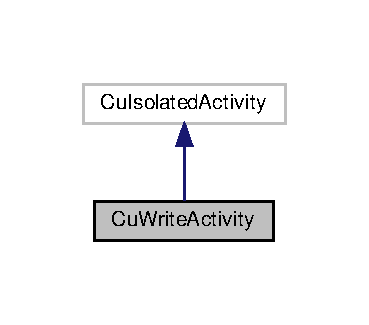
\includegraphics[width=177pt]{classCuWriteActivity__inherit__graph}
\end{center}
\end{figure}
\subsection*{Public Member Functions}
\begin{DoxyCompactItemize}
\item 
\textbf{ Cu\+Write\+Activity} (const Cu\+Data \&token, \textbf{ Cu\+Ep\+C\+A\+Service} $\ast$df)
\item 
virtual \textbf{ $\sim$\+Cu\+Write\+Activity} ()
\item 
void \textbf{ event} (Cu\+Activity\+Event $\ast$e)
\item 
bool \textbf{ matches} (const Cu\+Data \&token) const
\end{DoxyCompactItemize}
\subsection*{Protected Member Functions}
\begin{DoxyCompactItemize}
\item 
void \textbf{ init} ()
\item 
void \textbf{ execute} ()
\item 
void \textbf{ on\+Exit} ()
\end{DoxyCompactItemize}


\subsection{Constructor \& Destructor Documentation}
\mbox{\label{classCuWriteActivity_a0278f6c87765540946d578b9f9bd7d63}} 
\index{Cu\+Write\+Activity@{Cu\+Write\+Activity}!Cu\+Write\+Activity@{Cu\+Write\+Activity}}
\index{Cu\+Write\+Activity@{Cu\+Write\+Activity}!Cu\+Write\+Activity@{Cu\+Write\+Activity}}
\subsubsection{Cu\+Write\+Activity()}
{\footnotesize\ttfamily Cu\+Write\+Activity\+::\+Cu\+Write\+Activity (\begin{DoxyParamCaption}\item[{const Cu\+Data \&}]{token,  }\item[{\textbf{ Cu\+Ep\+C\+A\+Service} $\ast$}]{df }\end{DoxyParamCaption})}



References Cu\+Write\+Activity\+Private\+::epics\+\_\+service, Cu\+Write\+Activity\+Private\+::err, and Cu\+Write\+Activity\+Private\+::other\+\_\+thread\+\_\+id.

\mbox{\label{classCuWriteActivity_aef98deab4678b6d13b0597067427954f}} 
\index{Cu\+Write\+Activity@{Cu\+Write\+Activity}!````~Cu\+Write\+Activity@{$\sim$\+Cu\+Write\+Activity}}
\index{````~Cu\+Write\+Activity@{$\sim$\+Cu\+Write\+Activity}!Cu\+Write\+Activity@{Cu\+Write\+Activity}}
\subsubsection{$\sim$\+Cu\+Write\+Activity()}
{\footnotesize\ttfamily Cu\+Write\+Activity\+::$\sim$\+Cu\+Write\+Activity (\begin{DoxyParamCaption}{ }\end{DoxyParamCaption})\hspace{0.3cm}{\ttfamily [virtual]}}



\subsection{Member Function Documentation}
\mbox{\label{classCuWriteActivity_a7096f057f66631ea030f42fe9e817b6c}} 
\index{Cu\+Write\+Activity@{Cu\+Write\+Activity}!event@{event}}
\index{event@{event}!Cu\+Write\+Activity@{Cu\+Write\+Activity}}
\subsubsection{event()}
{\footnotesize\ttfamily void Cu\+Write\+Activity\+::event (\begin{DoxyParamCaption}\item[{Cu\+Activity\+Event $\ast$}]{e }\end{DoxyParamCaption})}

\mbox{\label{classCuWriteActivity_a6d8a87364002b18f420c9302c20d4a96}} 
\index{Cu\+Write\+Activity@{Cu\+Write\+Activity}!execute@{execute}}
\index{execute@{execute}!Cu\+Write\+Activity@{Cu\+Write\+Activity}}
\subsubsection{execute()}
{\footnotesize\ttfamily void Cu\+Write\+Activity\+::execute (\begin{DoxyParamCaption}{ }\end{DoxyParamCaption})\hspace{0.3cm}{\ttfamily [protected]}}



References Cu\+Write\+Activity\+Private\+::err, Cu\+Write\+Activity\+Private\+::msg, and Cu\+Write\+Activity\+Private\+::my\+\_\+thread\+\_\+id.

\mbox{\label{classCuWriteActivity_a0a0cde69cbe5f3e6dc1d633bf62fd204}} 
\index{Cu\+Write\+Activity@{Cu\+Write\+Activity}!init@{init}}
\index{init@{init}!Cu\+Write\+Activity@{Cu\+Write\+Activity}}
\subsubsection{init()}
{\footnotesize\ttfamily void Cu\+Write\+Activity\+::init (\begin{DoxyParamCaption}{ }\end{DoxyParamCaption})\hspace{0.3cm}{\ttfamily [protected]}}



References Cu\+Write\+Activity\+Private\+::my\+\_\+thread\+\_\+id, and Cu\+Write\+Activity\+Private\+::other\+\_\+thread\+\_\+id.

\mbox{\label{classCuWriteActivity_a6887775a9b2490d65541e67f9ac25e2b}} 
\index{Cu\+Write\+Activity@{Cu\+Write\+Activity}!matches@{matches}}
\index{matches@{matches}!Cu\+Write\+Activity@{Cu\+Write\+Activity}}
\subsubsection{matches()}
{\footnotesize\ttfamily bool Cu\+Write\+Activity\+::matches (\begin{DoxyParamCaption}\item[{const Cu\+Data \&}]{token }\end{DoxyParamCaption}) const}

\mbox{\label{classCuWriteActivity_a3266335817f6907435a8e9b3e54c36f6}} 
\index{Cu\+Write\+Activity@{Cu\+Write\+Activity}!on\+Exit@{on\+Exit}}
\index{on\+Exit@{on\+Exit}!Cu\+Write\+Activity@{Cu\+Write\+Activity}}
\subsubsection{on\+Exit()}
{\footnotesize\ttfamily void Cu\+Write\+Activity\+::on\+Exit (\begin{DoxyParamCaption}{ }\end{DoxyParamCaption})\hspace{0.3cm}{\ttfamily [protected]}}



References Cu\+Write\+Activity\+Private\+::err, Cu\+Epics\+World\+::fill\+Thread\+Info(), Cu\+Write\+Activity\+Private\+::msg, and Cu\+Write\+Activity\+Private\+::my\+\_\+thread\+\_\+id.



The documentation for this class was generated from the following files\+:\begin{DoxyCompactItemize}
\item 
\textbf{ cuputactivity.\+h}\item 
\textbf{ cuputactivity.\+cpp}\end{DoxyCompactItemize}

\section{Cu\+Write\+Activity\+Private Class Reference}
\label{classCuWriteActivityPrivate}\index{Cu\+Write\+Activity\+Private@{Cu\+Write\+Activity\+Private}}
\subsection*{Public Attributes}
\begin{DoxyCompactItemize}
\item 
\textbf{ Cu\+Ep\+C\+A\+Service} $\ast$ \textbf{ epics\+\_\+service}
\item 
std\+::string \textbf{ msg}
\item 
bool \textbf{ err}
\item 
pthread\+\_\+t \textbf{ my\+\_\+thread\+\_\+id}
\item 
pthread\+\_\+t \textbf{ other\+\_\+thread\+\_\+id}
\item 
Cu\+Data \textbf{ point\+\_\+info}
\end{DoxyCompactItemize}


\subsection{Member Data Documentation}
\mbox{\label{classCuWriteActivityPrivate_a53c62a50cd5c4bbae6ad887d01846831}} 
\index{Cu\+Write\+Activity\+Private@{Cu\+Write\+Activity\+Private}!epics\+\_\+service@{epics\+\_\+service}}
\index{epics\+\_\+service@{epics\+\_\+service}!Cu\+Write\+Activity\+Private@{Cu\+Write\+Activity\+Private}}
\subsubsection{epics\+\_\+service}
{\footnotesize\ttfamily \textbf{ Cu\+Ep\+C\+A\+Service}$\ast$ Cu\+Write\+Activity\+Private\+::epics\+\_\+service}



Referenced by Cu\+Write\+Activity\+::\+Cu\+Write\+Activity().

\mbox{\label{classCuWriteActivityPrivate_a885eca9c954ca5592b7d7cada294cd1e}} 
\index{Cu\+Write\+Activity\+Private@{Cu\+Write\+Activity\+Private}!err@{err}}
\index{err@{err}!Cu\+Write\+Activity\+Private@{Cu\+Write\+Activity\+Private}}
\subsubsection{err}
{\footnotesize\ttfamily bool Cu\+Write\+Activity\+Private\+::err}



Referenced by Cu\+Write\+Activity\+::\+Cu\+Write\+Activity(), Cu\+Write\+Activity\+::execute(), and Cu\+Write\+Activity\+::on\+Exit().

\mbox{\label{classCuWriteActivityPrivate_a84c08ce77441ed456685a0f2c8d6ac35}} 
\index{Cu\+Write\+Activity\+Private@{Cu\+Write\+Activity\+Private}!msg@{msg}}
\index{msg@{msg}!Cu\+Write\+Activity\+Private@{Cu\+Write\+Activity\+Private}}
\subsubsection{msg}
{\footnotesize\ttfamily std\+::string Cu\+Write\+Activity\+Private\+::msg}



Referenced by Cu\+Write\+Activity\+::execute(), and Cu\+Write\+Activity\+::on\+Exit().

\mbox{\label{classCuWriteActivityPrivate_a2a1bd9747fb88e389c4d7a0584fcdb8d}} 
\index{Cu\+Write\+Activity\+Private@{Cu\+Write\+Activity\+Private}!my\+\_\+thread\+\_\+id@{my\+\_\+thread\+\_\+id}}
\index{my\+\_\+thread\+\_\+id@{my\+\_\+thread\+\_\+id}!Cu\+Write\+Activity\+Private@{Cu\+Write\+Activity\+Private}}
\subsubsection{my\+\_\+thread\+\_\+id}
{\footnotesize\ttfamily pthread\+\_\+t Cu\+Write\+Activity\+Private\+::my\+\_\+thread\+\_\+id}



Referenced by Cu\+Write\+Activity\+::execute(), Cu\+Write\+Activity\+::init(), and Cu\+Write\+Activity\+::on\+Exit().

\mbox{\label{classCuWriteActivityPrivate_a166431d6df992d21599d7cfcdccdebc4}} 
\index{Cu\+Write\+Activity\+Private@{Cu\+Write\+Activity\+Private}!other\+\_\+thread\+\_\+id@{other\+\_\+thread\+\_\+id}}
\index{other\+\_\+thread\+\_\+id@{other\+\_\+thread\+\_\+id}!Cu\+Write\+Activity\+Private@{Cu\+Write\+Activity\+Private}}
\subsubsection{other\+\_\+thread\+\_\+id}
{\footnotesize\ttfamily pthread\+\_\+t Cu\+Write\+Activity\+Private\+::other\+\_\+thread\+\_\+id}



Referenced by Cu\+Write\+Activity\+::\+Cu\+Write\+Activity(), and Cu\+Write\+Activity\+::init().

\mbox{\label{classCuWriteActivityPrivate_a3b5730761a1b05648aebf80752cdafc7}} 
\index{Cu\+Write\+Activity\+Private@{Cu\+Write\+Activity\+Private}!point\+\_\+info@{point\+\_\+info}}
\index{point\+\_\+info@{point\+\_\+info}!Cu\+Write\+Activity\+Private@{Cu\+Write\+Activity\+Private}}
\subsubsection{point\+\_\+info}
{\footnotesize\ttfamily Cu\+Data Cu\+Write\+Activity\+Private\+::point\+\_\+info}



The documentation for this class was generated from the following file\+:\begin{DoxyCompactItemize}
\item 
\textbf{ cuputactivity.\+cpp}\end{DoxyCompactItemize}

\section{Ep\+Source Class Reference}
\label{classEpSource}\index{Ep\+Source@{Ep\+Source}}


{\ttfamily \#include $<$epsource.\+h$>$}

\subsection*{Public Types}
\begin{DoxyCompactItemize}
\item 
enum \textbf{ Type} \{ \textbf{ PV} = 0, 
\textbf{ Field}
 \}
\end{DoxyCompactItemize}
\subsection*{Public Member Functions}
\begin{DoxyCompactItemize}
\item 
\textbf{ Ep\+Source} ()
\item 
\textbf{ Ep\+Source} (const std\+::string s)
\item 
\textbf{ Ep\+Source} (const \textbf{ Ep\+Source} \&other)
\item 
string \textbf{ get\+I\+OC} () const
\item 
string \textbf{ get\+PV} () const
\item 
string \textbf{ get\+Field} () const
\item 
string \textbf{ get\+Name} () const
\item 
std\+::vector$<$ string $>$ \textbf{ get\+Args} () const
\item 
string \textbf{ to\+String} () const
\item 
\textbf{ Type} \textbf{ get\+Type} () const
\item 
\textbf{ Ep\+Source} \& \textbf{ operator=} (const \textbf{ Ep\+Source} \&other)
\item 
bool \textbf{ operator==} (const \textbf{ Ep\+Source} \&other) const
\item 
std\+::string \textbf{ get\+Args\+String} () const
\end{DoxyCompactItemize}


\subsection{Member Enumeration Documentation}
\mbox{\label{classEpSource_a85c6c6f7a918fdf85359a347cfe209a5}} 
\index{Ep\+Source@{Ep\+Source}!Type@{Type}}
\index{Type@{Type}!Ep\+Source@{Ep\+Source}}
\subsubsection{Type}
{\footnotesize\ttfamily enum \textbf{ Ep\+Source\+::\+Type}}

\begin{DoxyEnumFields}{Enumerator}
\raisebox{\heightof{T}}[0pt][0pt]{\index{PV@{PV}!Ep\+Source@{Ep\+Source}}\index{Ep\+Source@{Ep\+Source}!PV@{PV}}}\mbox{\label{classEpSource_a85c6c6f7a918fdf85359a347cfe209a5a7e382531e760b9ec5d2499b02d45b0e6}} 
PV&\\
\hline

\raisebox{\heightof{T}}[0pt][0pt]{\index{Field@{Field}!Ep\+Source@{Ep\+Source}}\index{Ep\+Source@{Ep\+Source}!Field@{Field}}}\mbox{\label{classEpSource_a85c6c6f7a918fdf85359a347cfe209a5a090e1c9f51b93f2bf5b62d93ebffbd0c}} 
Field&\\
\hline

\end{DoxyEnumFields}


\subsection{Constructor \& Destructor Documentation}
\mbox{\label{classEpSource_a085dc13a32d55cba76a96155c4c57207}} 
\index{Ep\+Source@{Ep\+Source}!Ep\+Source@{Ep\+Source}}
\index{Ep\+Source@{Ep\+Source}!Ep\+Source@{Ep\+Source}}
\subsubsection{Ep\+Source()\hspace{0.1cm}{\footnotesize\ttfamily [1/3]}}
{\footnotesize\ttfamily Ep\+Source\+::\+Ep\+Source (\begin{DoxyParamCaption}{ }\end{DoxyParamCaption})}

\mbox{\label{classEpSource_a0e907f68fb4a7a20ed11112a5b74277f}} 
\index{Ep\+Source@{Ep\+Source}!Ep\+Source@{Ep\+Source}}
\index{Ep\+Source@{Ep\+Source}!Ep\+Source@{Ep\+Source}}
\subsubsection{Ep\+Source()\hspace{0.1cm}{\footnotesize\ttfamily [2/3]}}
{\footnotesize\ttfamily Ep\+Source\+::\+Ep\+Source (\begin{DoxyParamCaption}\item[{const std\+::string}]{s }\end{DoxyParamCaption})}

\mbox{\label{classEpSource_ad864cc732e96dac5210e1ec703a863b4}} 
\index{Ep\+Source@{Ep\+Source}!Ep\+Source@{Ep\+Source}}
\index{Ep\+Source@{Ep\+Source}!Ep\+Source@{Ep\+Source}}
\subsubsection{Ep\+Source()\hspace{0.1cm}{\footnotesize\ttfamily [3/3]}}
{\footnotesize\ttfamily Ep\+Source\+::\+Ep\+Source (\begin{DoxyParamCaption}\item[{const \textbf{ Ep\+Source} \&}]{other }\end{DoxyParamCaption})}



\subsection{Member Function Documentation}
\mbox{\label{classEpSource_a4ceeafa8be0982d354ae4f48ffa4c8c7}} 
\index{Ep\+Source@{Ep\+Source}!get\+Args@{get\+Args}}
\index{get\+Args@{get\+Args}!Ep\+Source@{Ep\+Source}}
\subsubsection{get\+Args()}
{\footnotesize\ttfamily std\+::vector$<$ string $>$ Ep\+Source\+::get\+Args (\begin{DoxyParamCaption}{ }\end{DoxyParamCaption}) const}



References get\+Args\+String().

\mbox{\label{classEpSource_a326fec362bb4eb57b5bb48cc4ed49cc5}} 
\index{Ep\+Source@{Ep\+Source}!get\+Args\+String@{get\+Args\+String}}
\index{get\+Args\+String@{get\+Args\+String}!Ep\+Source@{Ep\+Source}}
\subsubsection{get\+Args\+String()}
{\footnotesize\ttfamily std\+::string Ep\+Source\+::get\+Args\+String (\begin{DoxyParamCaption}{ }\end{DoxyParamCaption}) const}



Referenced by get\+Args(), and to\+String().

\mbox{\label{classEpSource_a9f683f46d4eccd3b2188641aa428af5e}} 
\index{Ep\+Source@{Ep\+Source}!get\+Field@{get\+Field}}
\index{get\+Field@{get\+Field}!Ep\+Source@{Ep\+Source}}
\subsubsection{get\+Field()}
{\footnotesize\ttfamily string Ep\+Source\+::get\+Field (\begin{DoxyParamCaption}{ }\end{DoxyParamCaption}) const}

\mbox{\label{classEpSource_a02247d03c99709ce0953e410f771faba}} 
\index{Ep\+Source@{Ep\+Source}!get\+I\+OC@{get\+I\+OC}}
\index{get\+I\+OC@{get\+I\+OC}!Ep\+Source@{Ep\+Source}}
\subsubsection{get\+I\+O\+C()}
{\footnotesize\ttfamily string Ep\+Source\+::get\+I\+OC (\begin{DoxyParamCaption}{ }\end{DoxyParamCaption}) const}



Referenced by Cu\+Put\+::start(), Cu\+Ep\+Configuration\+::start(), and to\+String().

\mbox{\label{classEpSource_a86cb212076d70e189f4e4f4abcc5363c}} 
\index{Ep\+Source@{Ep\+Source}!get\+Name@{get\+Name}}
\index{get\+Name@{get\+Name}!Ep\+Source@{Ep\+Source}}
\subsubsection{get\+Name()}
{\footnotesize\ttfamily string Ep\+Source\+::get\+Name (\begin{DoxyParamCaption}{ }\end{DoxyParamCaption}) const}



Referenced by Cu\+Put\+::get\+Token(), Cu\+Ep\+Configuration\+::get\+Token(), Cu\+Monitor\+::get\+Token(), Cu\+Put\+::on\+Result(), Cu\+Ep\+Configuration\+::on\+Result(), Cu\+Monitor\+::on\+Result(), Cu\+Put\+::start(), and Cu\+Ep\+Configuration\+::start().

\mbox{\label{classEpSource_a27eaf4b50e154bdc521dbe7489e5b889}} 
\index{Ep\+Source@{Ep\+Source}!get\+PV@{get\+PV}}
\index{get\+PV@{get\+PV}!Ep\+Source@{Ep\+Source}}
\subsubsection{get\+P\+V()}
{\footnotesize\ttfamily string Ep\+Source\+::get\+PV (\begin{DoxyParamCaption}{ }\end{DoxyParamCaption}) const}



Referenced by Cu\+Put\+::start(), Cu\+Ep\+Configuration\+::start(), and to\+String().

\mbox{\label{classEpSource_a40cb9e162b05d1272b8330d9f6aef4c2}} 
\index{Ep\+Source@{Ep\+Source}!get\+Type@{get\+Type}}
\index{get\+Type@{get\+Type}!Ep\+Source@{Ep\+Source}}
\subsubsection{get\+Type()}
{\footnotesize\ttfamily \textbf{ Ep\+Source\+::\+Type} Ep\+Source\+::get\+Type (\begin{DoxyParamCaption}{ }\end{DoxyParamCaption}) const}



References Field, and PV.



Referenced by Cu\+Put\+::start(), Cu\+Ep\+Configuration\+::start(), and to\+String().

\mbox{\label{classEpSource_ac1ecad9470b6cf4277d6d6d4f250f8ac}} 
\index{Ep\+Source@{Ep\+Source}!operator=@{operator=}}
\index{operator=@{operator=}!Ep\+Source@{Ep\+Source}}
\subsubsection{operator=()}
{\footnotesize\ttfamily \textbf{ Ep\+Source} \& Ep\+Source\+::operator= (\begin{DoxyParamCaption}\item[{const \textbf{ Ep\+Source} \&}]{other }\end{DoxyParamCaption})}

\mbox{\label{classEpSource_a7cb2815e80216a7a287b3e9d0c5780c5}} 
\index{Ep\+Source@{Ep\+Source}!operator==@{operator==}}
\index{operator==@{operator==}!Ep\+Source@{Ep\+Source}}
\subsubsection{operator==()}
{\footnotesize\ttfamily bool Ep\+Source\+::operator== (\begin{DoxyParamCaption}\item[{const \textbf{ Ep\+Source} \&}]{other }\end{DoxyParamCaption}) const}

\mbox{\label{classEpSource_a97a1c3a5baf6b530339f583e51439a55}} 
\index{Ep\+Source@{Ep\+Source}!to\+String@{to\+String}}
\index{to\+String@{to\+String}!Ep\+Source@{Ep\+Source}}
\subsubsection{to\+String()}
{\footnotesize\ttfamily std\+::string Ep\+Source\+::to\+String (\begin{DoxyParamCaption}{ }\end{DoxyParamCaption}) const}



References get\+Args\+String(), get\+I\+O\+C(), get\+P\+V(), get\+Type(), and PV.



The documentation for this class was generated from the following files\+:\begin{DoxyCompactItemize}
\item 
\textbf{ epsource.\+h}\item 
\textbf{ epsource.\+cpp}\end{DoxyCompactItemize}

\chapter{File Documentation}
\section{cuepactionfactories.\+cpp File Reference}
\label{cuepactionfactories_8cpp}\index{cuepactionfactories.\+cpp@{cuepactionfactories.\+cpp}}
{\ttfamily \#include \char`\"{}cuepactionfactories.\+h\char`\"{}}\newline
{\ttfamily \#include \char`\"{}cumonitor.\+h\char`\"{}}\newline
{\ttfamily \#include \char`\"{}cuput.\+h\char`\"{}}\newline
{\ttfamily \#include \char`\"{}cuepconfiguration.\+h\char`\"{}}\newline
{\ttfamily \#include $<$cumacros.\+h$>$}\newline
{\ttfamily \#include $<$cadef.\+h$>$}\newline
{\ttfamily \#include $<$cudata.\+h$>$}\newline
Include dependency graph for cuepactionfactories.\+cpp\+:\nopagebreak
\begin{figure}[H]
\begin{center}
\leavevmode
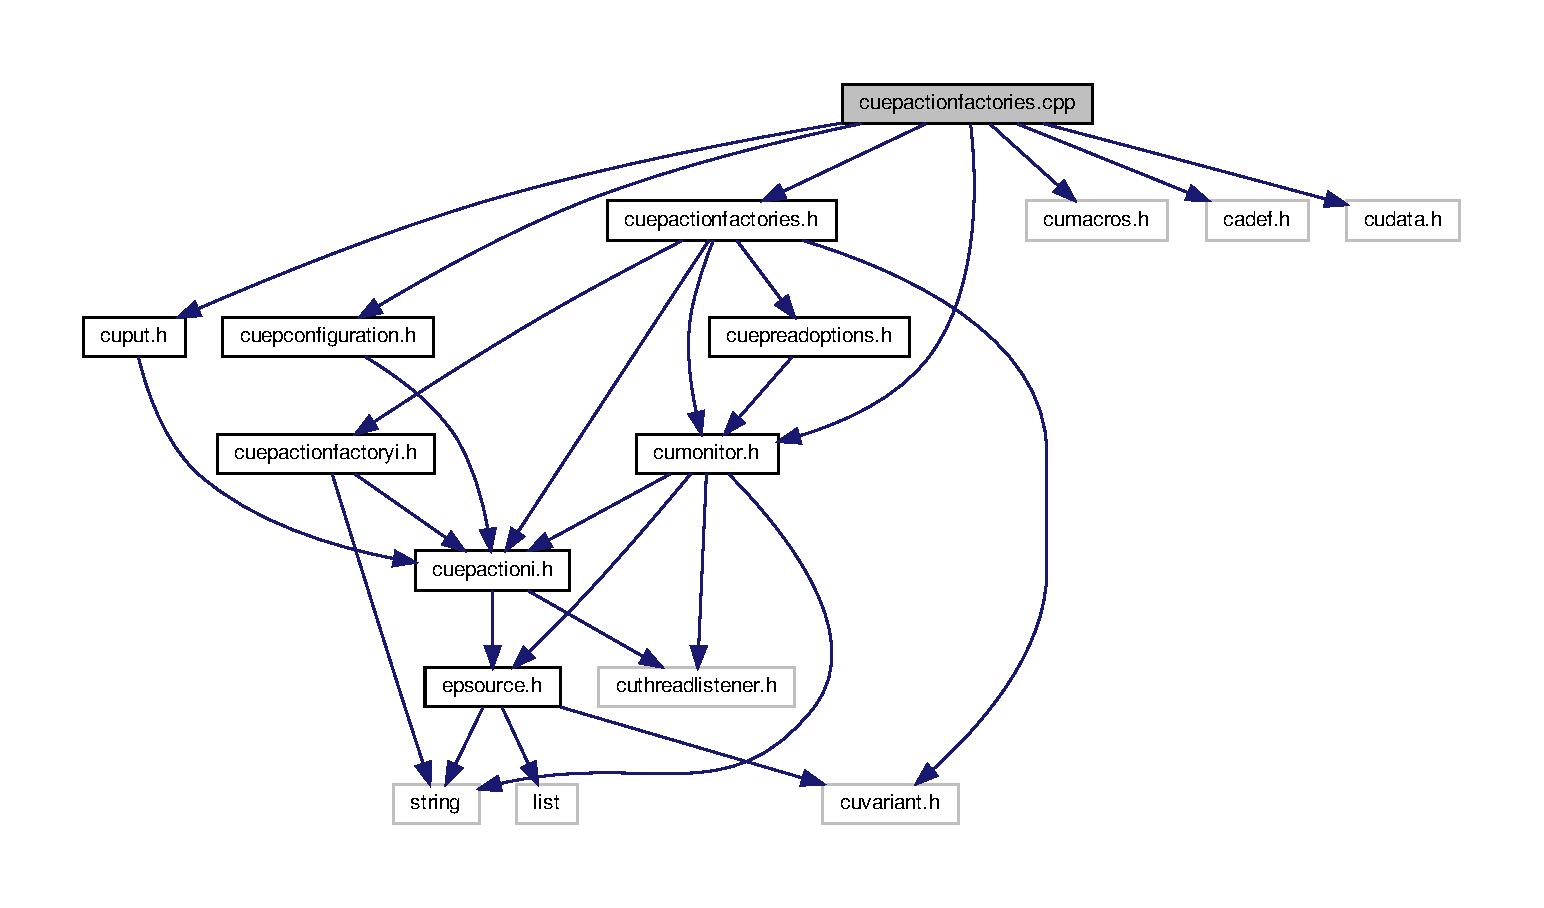
\includegraphics[width=350pt]{cuepactionfactories_8cpp__incl}
\end{center}
\end{figure}

\section{cuepactionfactories.\+h File Reference}
\label{cuepactionfactories_8h}\index{cuepactionfactories.\+h@{cuepactionfactories.\+h}}
{\ttfamily \#include $<$cuepactionfactoryi.\+h$>$}\newline
{\ttfamily \#include $<$cuepactioni.\+h$>$}\newline
{\ttfamily \#include $<$cuvariant.\+h$>$}\newline
{\ttfamily \#include $<$cumonitor.\+h$>$}\newline
{\ttfamily \#include $<$cuepreadoptions.\+h$>$}\newline
Include dependency graph for cuepactionfactories.\+h\+:\nopagebreak
\begin{figure}[H]
\begin{center}
\leavevmode
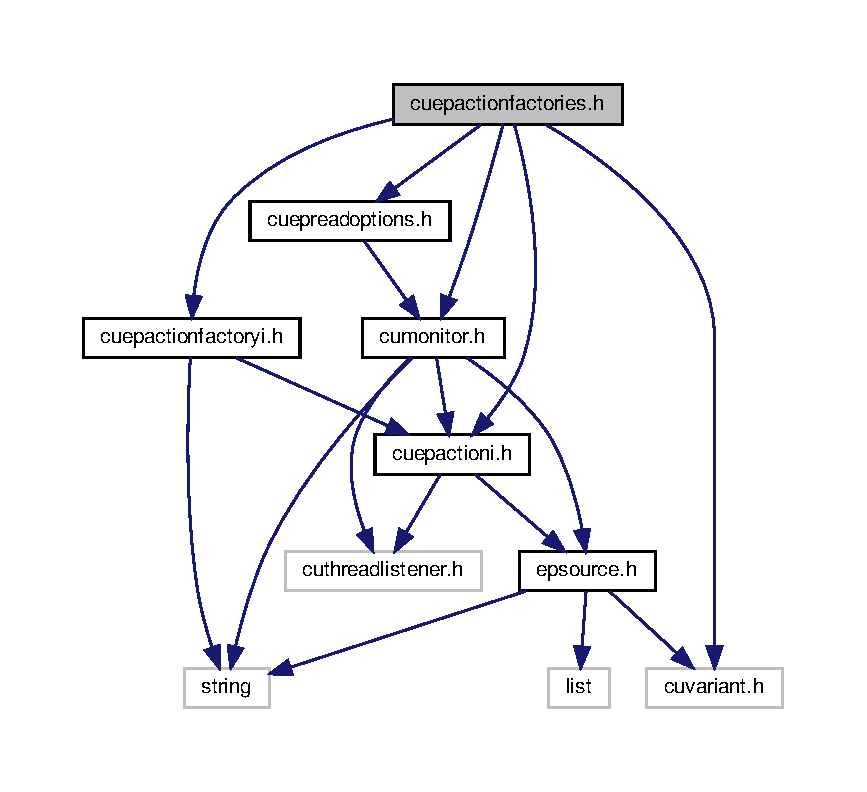
\includegraphics[width=350pt]{cuepactionfactories_8h__incl}
\end{center}
\end{figure}
This graph shows which files directly or indirectly include this file\+:\nopagebreak
\begin{figure}[H]
\begin{center}
\leavevmode
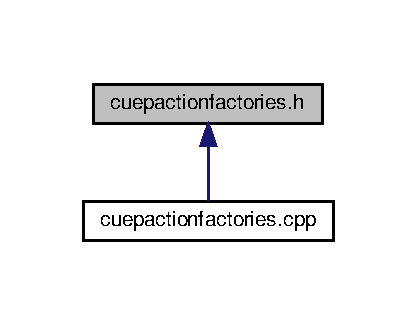
\includegraphics[width=200pt]{cuepactionfactories_8h__dep__incl}
\end{center}
\end{figure}
\subsection*{Classes}
\begin{DoxyCompactItemize}
\item 
class \textbf{ Cu\+Epics\+Reader\+Factory}
\item 
class \textbf{ Cu\+Epics\+Writer\+Factory}
\item 
class \textbf{ Cu\+Epics\+Att\+Conf\+Factory}
\end{DoxyCompactItemize}

\section{cuepactionfactoryi.\+h File Reference}
\label{cuepactionfactoryi_8h}\index{cuepactionfactoryi.\+h@{cuepactionfactoryi.\+h}}
{\ttfamily \#include $<$string$>$}\newline
{\ttfamily \#include $<$cuepactioni.\+h$>$}\newline
Include dependency graph for cuepactionfactoryi.\+h\+:\nopagebreak
\begin{figure}[H]
\begin{center}
\leavevmode
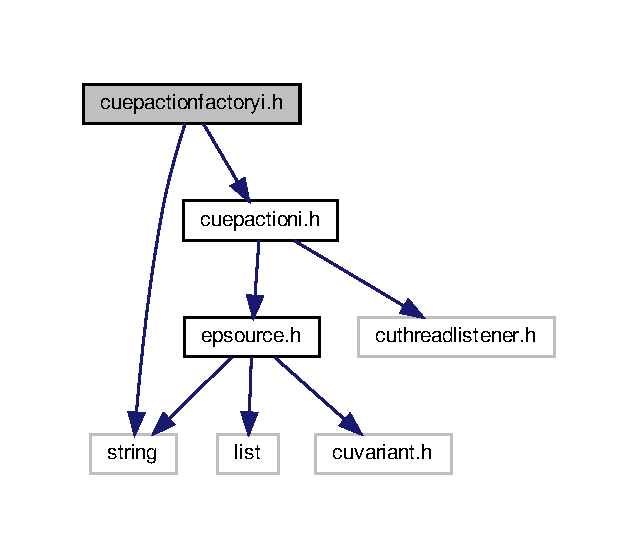
\includegraphics[width=306pt]{cuepactionfactoryi_8h__incl}
\end{center}
\end{figure}
This graph shows which files directly or indirectly include this file\+:\nopagebreak
\begin{figure}[H]
\begin{center}
\leavevmode
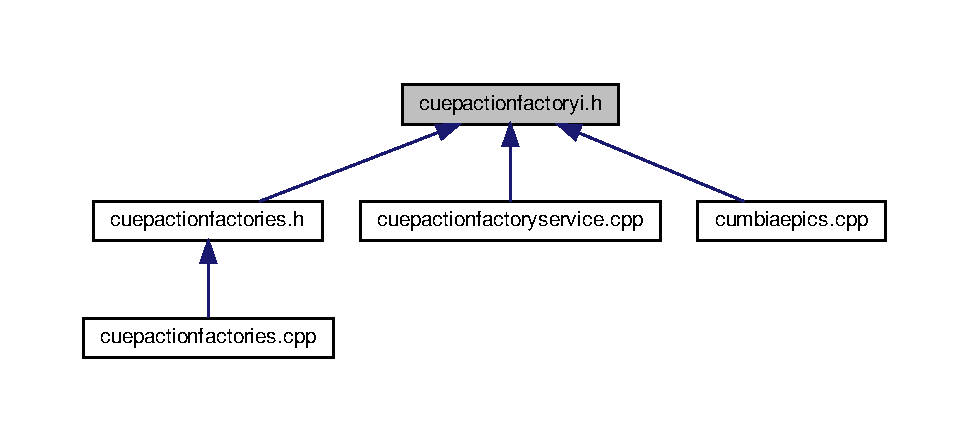
\includegraphics[width=350pt]{cuepactionfactoryi_8h__dep__incl}
\end{center}
\end{figure}
\subsection*{Classes}
\begin{DoxyCompactItemize}
\item 
class \textbf{ Cu\+Epics\+Action\+FactoryI}
\end{DoxyCompactItemize}

\section{cuepactionfactoryservice.\+cpp File Reference}
\label{cuepactionfactoryservice_8cpp}\index{cuepactionfactoryservice.\+cpp@{cuepactionfactoryservice.\+cpp}}
{\ttfamily \#include \char`\"{}cuepactionfactoryi.\+h\char`\"{}}\newline
{\ttfamily \#include \char`\"{}cuepactionfactoryservice.\+h\char`\"{}}\newline
{\ttfamily \#include \char`\"{}cuepics-\/world.\+h\char`\"{}}\newline
{\ttfamily \#include \char`\"{}epsource.\+h\char`\"{}}\newline
{\ttfamily \#include \char`\"{}cuepactioni.\+h\char`\"{}}\newline
{\ttfamily \#include $<$culog.\+h$>$}\newline
{\ttfamily \#include $<$cadef.\+h$>$}\newline
{\ttfamily \#include $<$map$>$}\newline
{\ttfamily \#include $<$mutex$>$}\newline
{\ttfamily \#include $<$cumacros.\+h$>$}\newline
Include dependency graph for cuepactionfactoryservice.\+cpp\+:\nopagebreak
\begin{figure}[H]
\begin{center}
\leavevmode
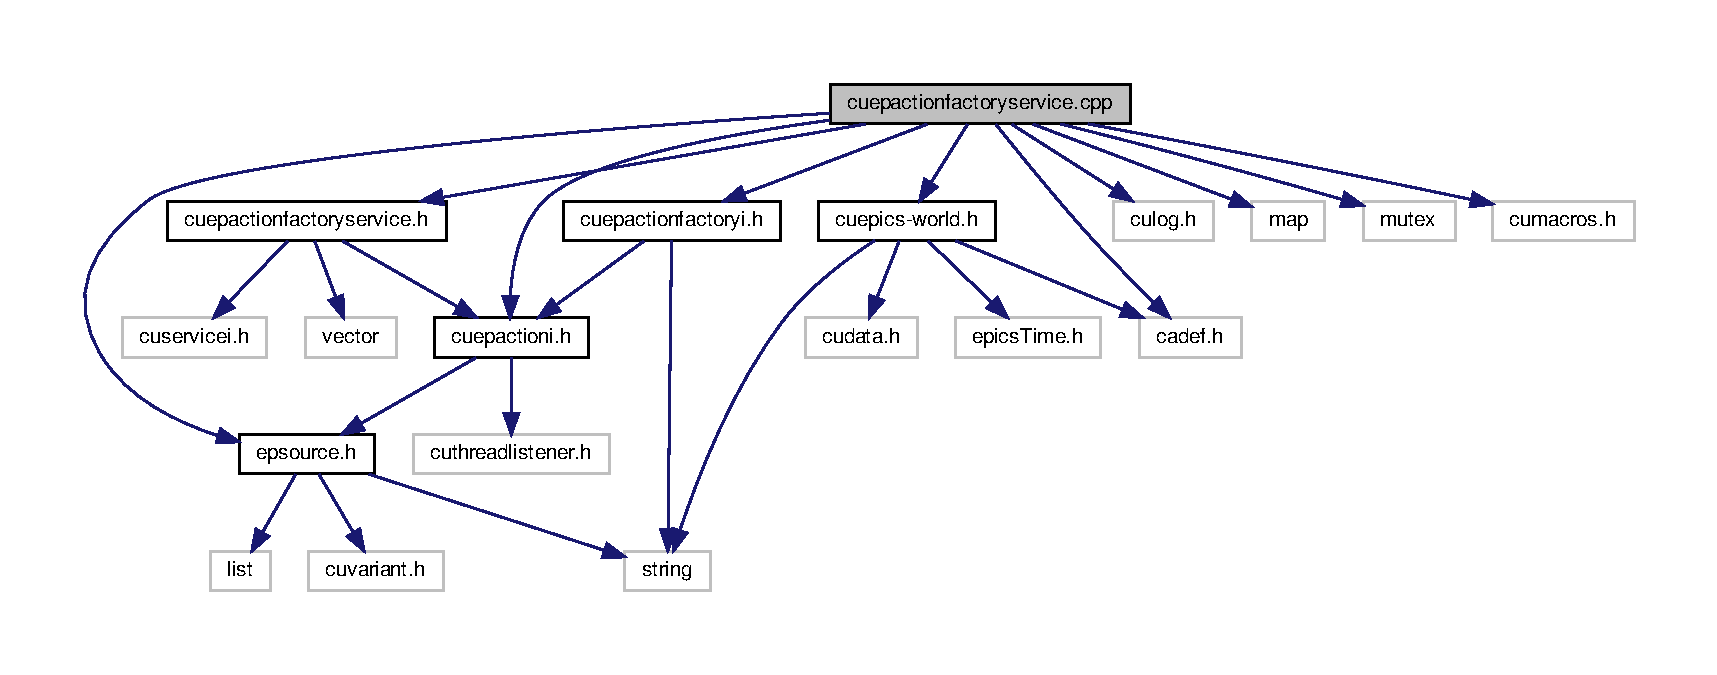
\includegraphics[width=350pt]{cuepactionfactoryservice_8cpp__incl}
\end{center}
\end{figure}
\subsection*{Classes}
\begin{DoxyCompactItemize}
\item 
class \textbf{ Cu\+Action\+Factory\+Service\+Private}
\end{DoxyCompactItemize}

\section{cuepactionfactoryservice.\+h File Reference}
\label{cuepactionfactoryservice_8h}\index{cuepactionfactoryservice.\+h@{cuepactionfactoryservice.\+h}}
{\ttfamily \#include $<$cuservicei.\+h$>$}\newline
{\ttfamily \#include $<$cuepactioni.\+h$>$}\newline
{\ttfamily \#include $<$vector$>$}\newline
Include dependency graph for cuepactionfactoryservice.\+h\+:\nopagebreak
\begin{figure}[H]
\begin{center}
\leavevmode
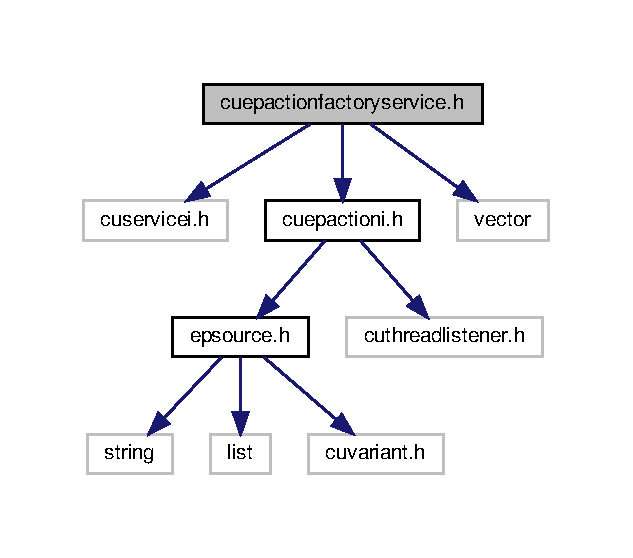
\includegraphics[width=304pt]{cuepactionfactoryservice_8h__incl}
\end{center}
\end{figure}
This graph shows which files directly or indirectly include this file\+:\nopagebreak
\begin{figure}[H]
\begin{center}
\leavevmode
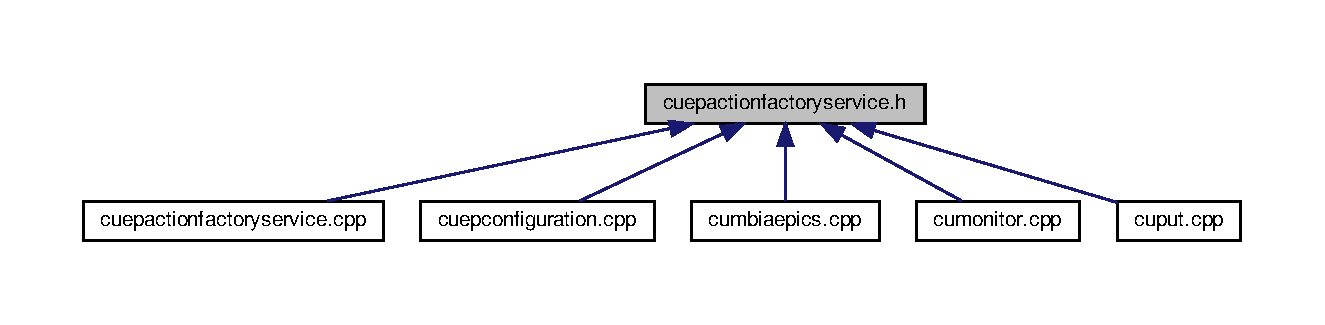
\includegraphics[width=350pt]{cuepactionfactoryservice_8h__dep__incl}
\end{center}
\end{figure}
\subsection*{Classes}
\begin{DoxyCompactItemize}
\item 
class \textbf{ Cu\+Action\+Factory\+Service}
\end{DoxyCompactItemize}

\section{cuepactioni.\+cpp File Reference}
\label{cuepactioni_8cpp}\index{cuepactioni.\+cpp@{cuepactioni.\+cpp}}
{\ttfamily \#include \char`\"{}cuepactioni.\+h\char`\"{}}\newline
Include dependency graph for cuepactioni.\+cpp\+:\nopagebreak
\begin{figure}[H]
\begin{center}
\leavevmode
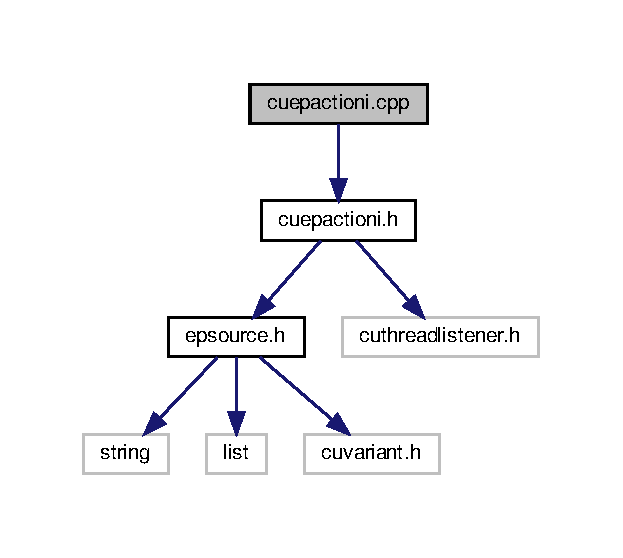
\includegraphics[width=299pt]{cuepactioni_8cpp__incl}
\end{center}
\end{figure}

\section{cuepactioni.\+h File Reference}
\label{cuepactioni_8h}\index{cuepactioni.\+h@{cuepactioni.\+h}}
{\ttfamily \#include $<$epsource.\+h$>$}\newline
{\ttfamily \#include $<$cuthreadlistener.\+h$>$}\newline
Include dependency graph for cuepactioni.\+h\+:\nopagebreak
\begin{figure}[H]
\begin{center}
\leavevmode
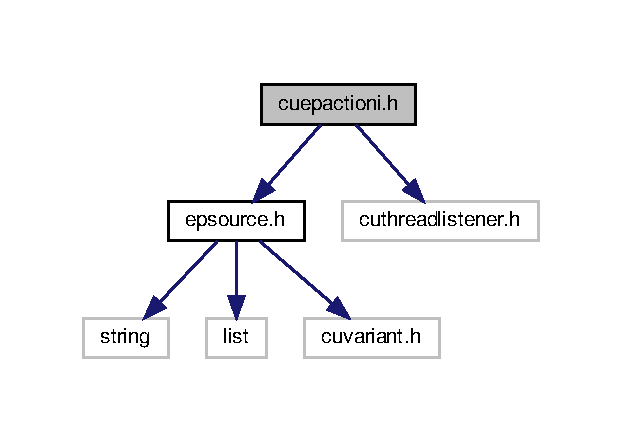
\includegraphics[width=299pt]{cuepactioni_8h__incl}
\end{center}
\end{figure}
This graph shows which files directly or indirectly include this file\+:\nopagebreak
\begin{figure}[H]
\begin{center}
\leavevmode
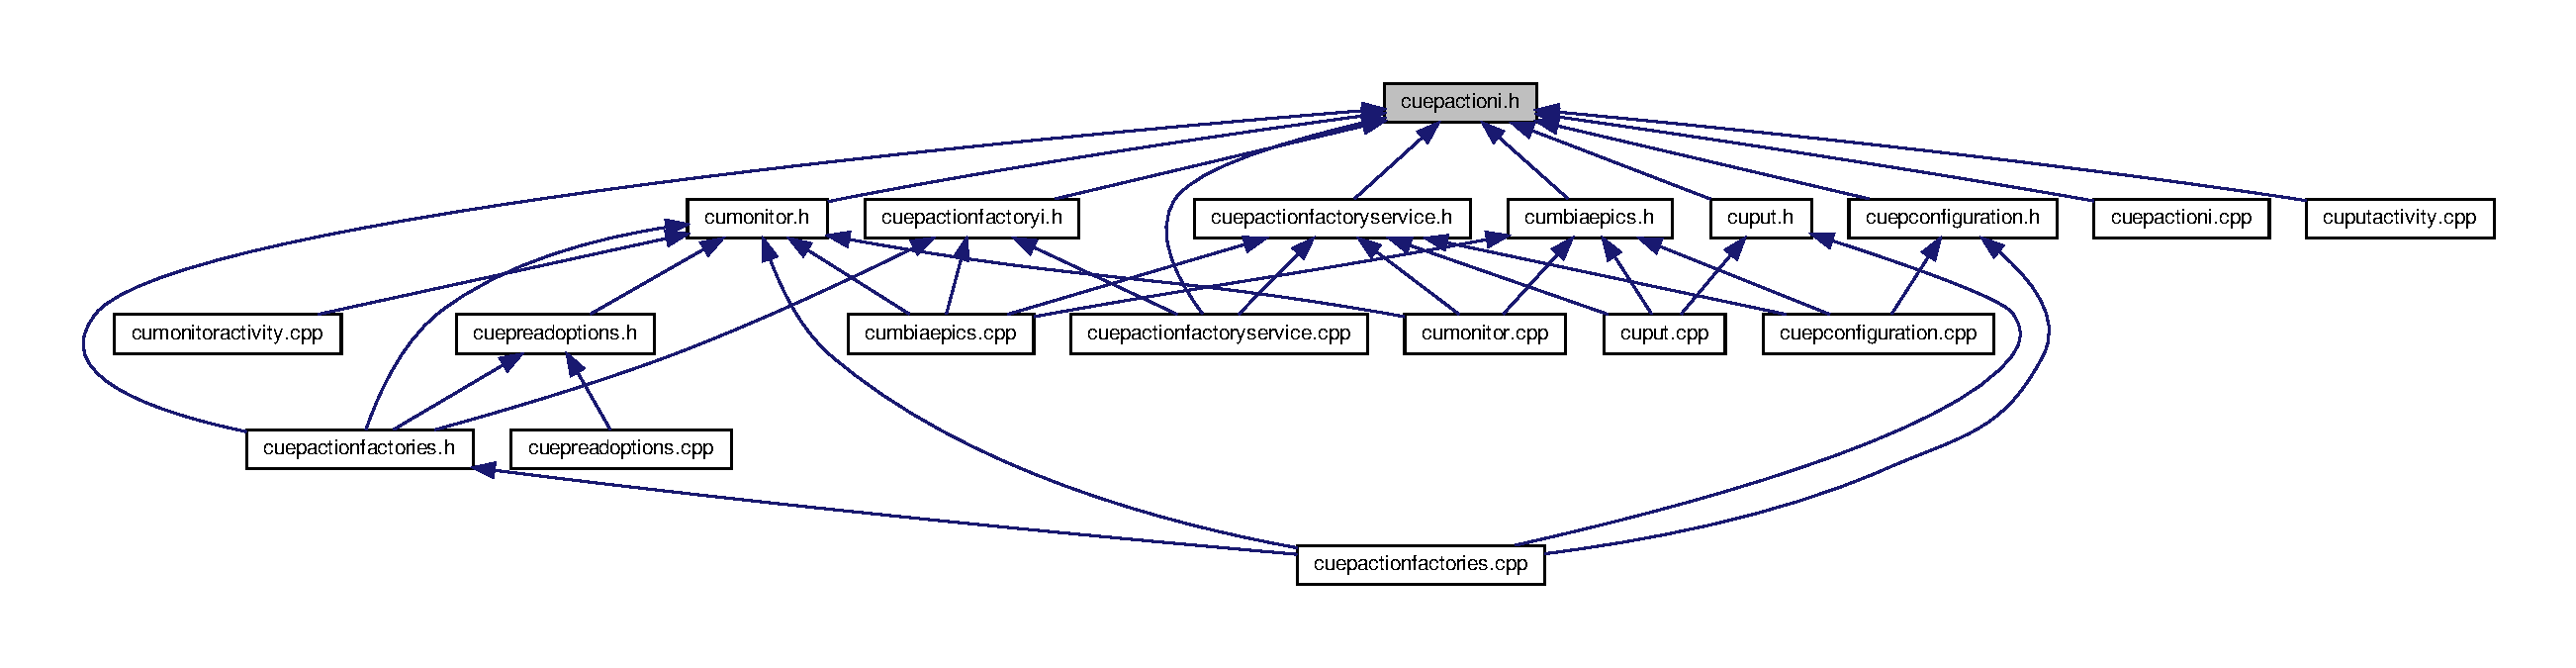
\includegraphics[width=350pt]{cuepactioni_8h__dep__incl}
\end{center}
\end{figure}
\subsection*{Classes}
\begin{DoxyCompactItemize}
\item 
class \textbf{ Cu\+Epics\+ActionI}
\begin{DoxyCompactList}\small\item\em an interface for an E\+P\+I\+CS {\itshape action}, as a reader (implemented) or a writer (not yet implemented) \end{DoxyCompactList}\end{DoxyCompactItemize}

\section{cuepcaservice.\+cpp File Reference}
\label{cuepcaservice_8cpp}\index{cuepcaservice.\+cpp@{cuepcaservice.\+cpp}}
{\ttfamily \#include \char`\"{}cuepcaservice.\+h\char`\"{}}\newline
{\ttfamily \#include $<$mutex$>$}\newline
{\ttfamily \#include $<$cumacros.\+h$>$}\newline
{\ttfamily \#include \char`\"{}epsource.\+h\char`\"{}}\newline
{\ttfamily \#include $<$cadef.\+h$>$}\newline
Include dependency graph for cuepcaservice.\+cpp\+:\nopagebreak
\begin{figure}[H]
\begin{center}
\leavevmode
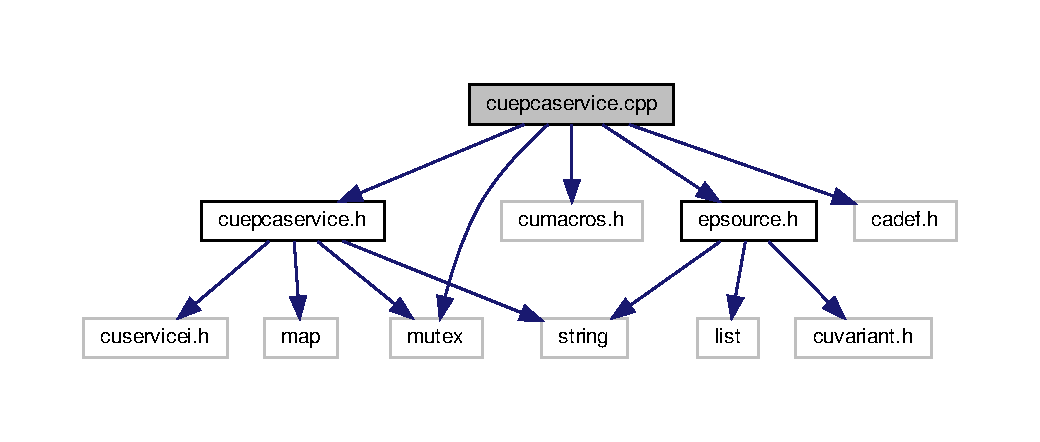
\includegraphics[width=350pt]{cuepcaservice_8cpp__incl}
\end{center}
\end{figure}

\section{cuepcaservice.\+h File Reference}
\label{cuepcaservice_8h}\index{cuepcaservice.\+h@{cuepcaservice.\+h}}
{\ttfamily \#include $<$cuservicei.\+h$>$}\newline
{\ttfamily \#include $<$map$>$}\newline
{\ttfamily \#include $<$string$>$}\newline
{\ttfamily \#include $<$mutex$>$}\newline
Include dependency graph for cuepcaservice.\+h\+:\nopagebreak
\begin{figure}[H]
\begin{center}
\leavevmode
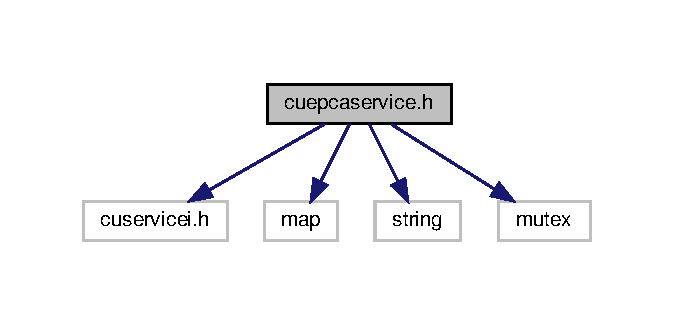
\includegraphics[width=324pt]{cuepcaservice_8h__incl}
\end{center}
\end{figure}
This graph shows which files directly or indirectly include this file\+:\nopagebreak
\begin{figure}[H]
\begin{center}
\leavevmode
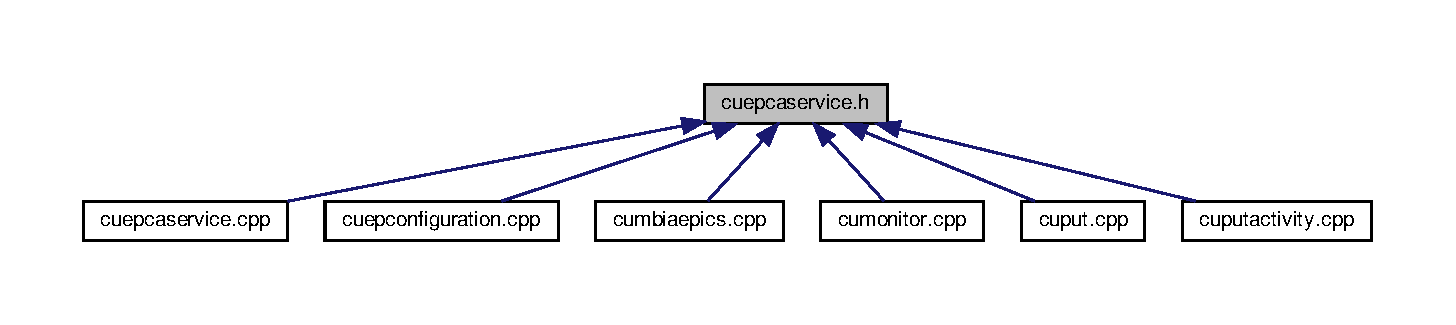
\includegraphics[width=350pt]{cuepcaservice_8h__dep__incl}
\end{center}
\end{figure}
\subsection*{Classes}
\begin{DoxyCompactItemize}
\item 
class \textbf{ Cu\+Ep\+C\+A\+Service}
\end{DoxyCompactItemize}

\section{cuepconfigactivity.\+cpp File Reference}
\label{cuepconfigactivity_8cpp}\index{cuepconfigactivity.\+cpp@{cuepconfigactivity.\+cpp}}
{\ttfamily \#include \char`\"{}cuepconfigactivity.\+h\char`\"{}}\newline
{\ttfamily \#include $<$cumacros.\+h$>$}\newline
{\ttfamily \#include \char`\"{}cuepics-\/world.\+h\char`\"{}}\newline
Include dependency graph for cuepconfigactivity.\+cpp\+:\nopagebreak
\begin{figure}[H]
\begin{center}
\leavevmode
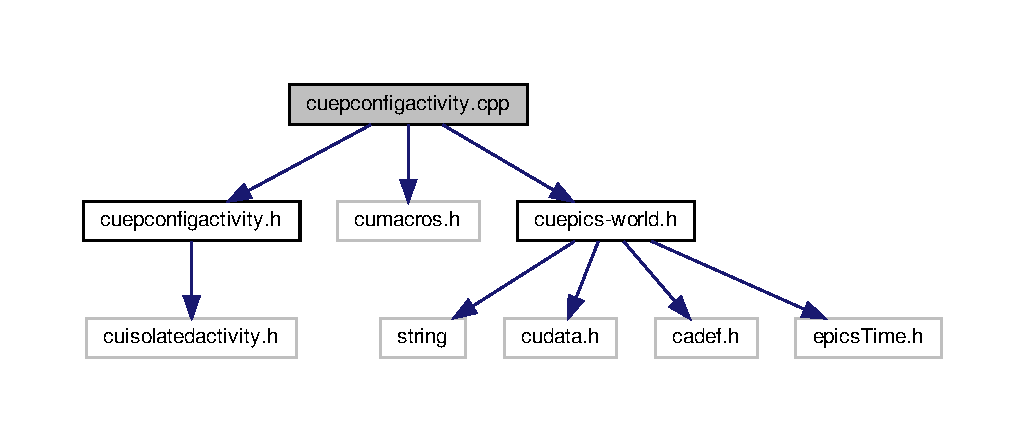
\includegraphics[width=350pt]{cuepconfigactivity_8cpp__incl}
\end{center}
\end{figure}
\subsection*{Classes}
\begin{DoxyCompactItemize}
\item 
class \textbf{ Cu\+Ep\+Config\+Activity\+Private}
\end{DoxyCompactItemize}

\section{cuepconfigactivity.\+h File Reference}
\label{cuepconfigactivity_8h}\index{cuepconfigactivity.\+h@{cuepconfigactivity.\+h}}
{\ttfamily \#include $<$cuisolatedactivity.\+h$>$}\newline
Include dependency graph for cuepconfigactivity.\+h\+:\nopagebreak
\begin{figure}[H]
\begin{center}
\leavevmode
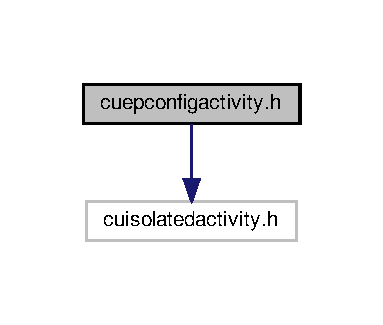
\includegraphics[width=184pt]{cuepconfigactivity_8h__incl}
\end{center}
\end{figure}
This graph shows which files directly or indirectly include this file\+:\nopagebreak
\begin{figure}[H]
\begin{center}
\leavevmode
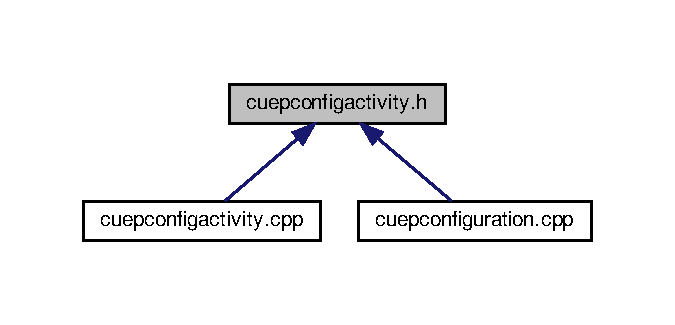
\includegraphics[width=324pt]{cuepconfigactivity_8h__dep__incl}
\end{center}
\end{figure}
\subsection*{Classes}
\begin{DoxyCompactItemize}
\item 
class \textbf{ Cu\+Ep\+Config\+Activity}
\end{DoxyCompactItemize}

\section{cuepconfiguration.\+cpp File Reference}
\label{cuepconfiguration_8cpp}\index{cuepconfiguration.\+cpp@{cuepconfiguration.\+cpp}}
{\ttfamily \#include \char`\"{}cuepconfiguration.\+h\char`\"{}}\newline
{\ttfamily \#include $<$culog.\+h$>$}\newline
{\ttfamily \#include $<$cumbiaepics.\+h$>$}\newline
{\ttfamily \#include $<$cumacros.\+h$>$}\newline
{\ttfamily \#include $<$cuserviceprovider.\+h$>$}\newline
{\ttfamily \#include \char`\"{}epsource.\+h\char`\"{}}\newline
{\ttfamily \#include $<$cuactivity.\+h$>$}\newline
{\ttfamily \#include \char`\"{}cuepcaservice.\+h\char`\"{}}\newline
{\ttfamily \#include \char`\"{}cuepconfigactivity.\+h\char`\"{}}\newline
{\ttfamily \#include \char`\"{}cuepactionfactoryservice.\+h\char`\"{}}\newline
{\ttfamily \#include \char`\"{}cudatalistener.\+h\char`\"{}}\newline
Include dependency graph for cuepconfiguration.\+cpp\+:\nopagebreak
\begin{figure}[H]
\begin{center}
\leavevmode
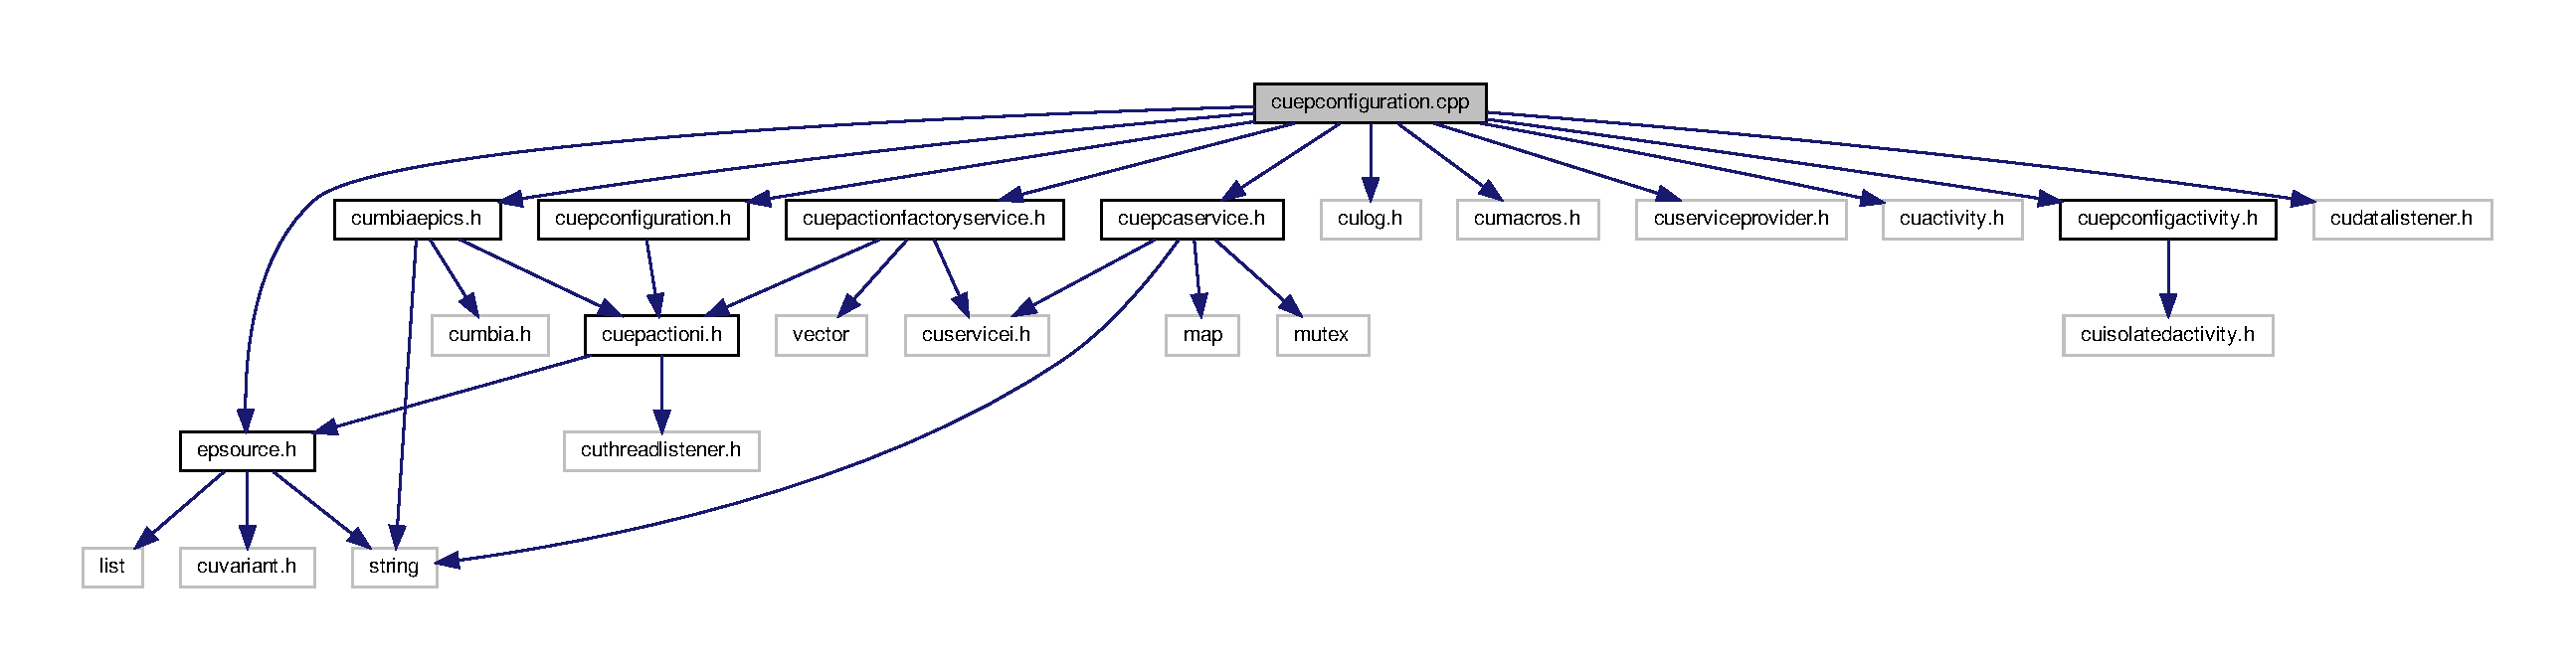
\includegraphics[width=350pt]{cuepconfiguration_8cpp__incl}
\end{center}
\end{figure}
\subsection*{Classes}
\begin{DoxyCompactItemize}
\item 
class \textbf{ Cu\+T\+Att\+Configuration\+Private}
\end{DoxyCompactItemize}

\section{cuepconfiguration.\+h File Reference}
\label{cuepconfiguration_8h}\index{cuepconfiguration.\+h@{cuepconfiguration.\+h}}
{\ttfamily \#include $<$cuepactioni.\+h$>$}\newline
Include dependency graph for cuepconfiguration.\+h\+:\nopagebreak
\begin{figure}[H]
\begin{center}
\leavevmode
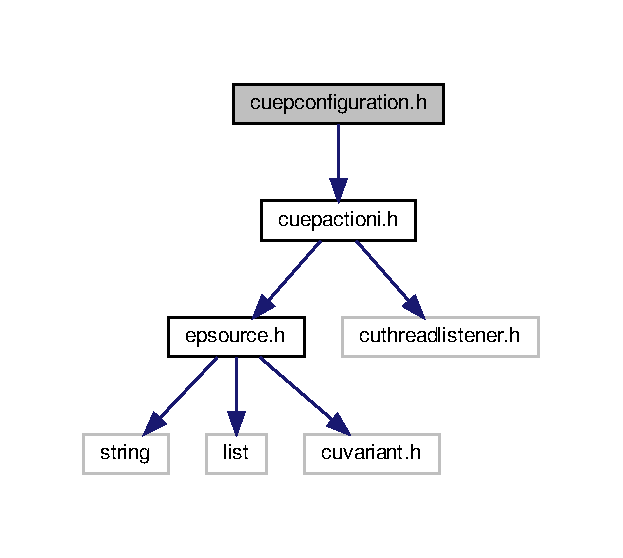
\includegraphics[width=299pt]{cuepconfiguration_8h__incl}
\end{center}
\end{figure}
This graph shows which files directly or indirectly include this file\+:\nopagebreak
\begin{figure}[H]
\begin{center}
\leavevmode
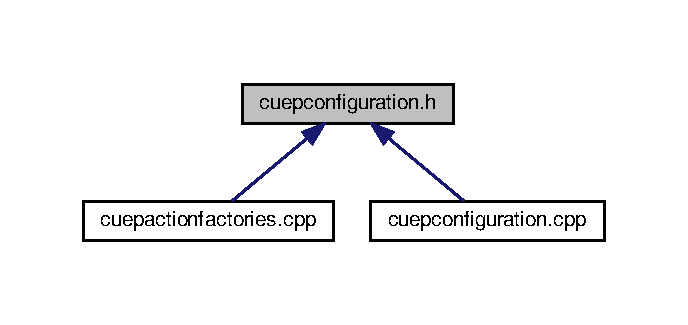
\includegraphics[width=330pt]{cuepconfiguration_8h__dep__incl}
\end{center}
\end{figure}
\subsection*{Classes}
\begin{DoxyCompactItemize}
\item 
class \textbf{ Cu\+Ep\+Configuration}
\end{DoxyCompactItemize}

\section{cuepics-\/world-\/config.cpp File Reference}
\label{cuepics-world-config_8cpp}\index{cuepics-\/world-\/config.\+cpp@{cuepics-\/world-\/config.\+cpp}}
{\ttfamily \#include \char`\"{}cuepics-\/world-\/config.\+h\char`\"{}}\newline
Include dependency graph for cuepics-\/world-\/config.cpp\+:\nopagebreak
\begin{figure}[H]
\begin{center}
\leavevmode
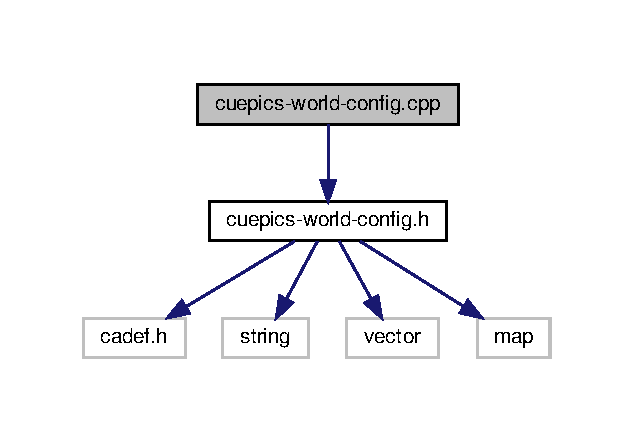
\includegraphics[width=304pt]{cuepics-world-config_8cpp__incl}
\end{center}
\end{figure}
\subsection*{Classes}
\begin{DoxyCompactItemize}
\item 
class \textbf{ Cu\+Epics\+World\+Config\+Private}
\end{DoxyCompactItemize}

\section{cuepics-\/world-\/config.h File Reference}
\label{cuepics-world-config_8h}\index{cuepics-\/world-\/config.\+h@{cuepics-\/world-\/config.\+h}}
{\ttfamily \#include $<$cadef.\+h$>$}\newline
{\ttfamily \#include $<$string$>$}\newline
{\ttfamily \#include $<$vector$>$}\newline
{\ttfamily \#include $<$map$>$}\newline
Include dependency graph for cuepics-\/world-\/config.h\+:\nopagebreak
\begin{figure}[H]
\begin{center}
\leavevmode
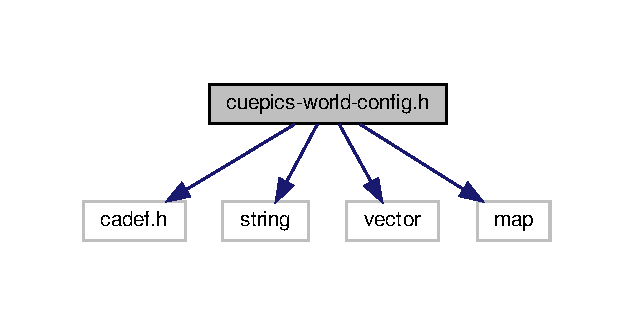
\includegraphics[width=304pt]{cuepics-world-config_8h__incl}
\end{center}
\end{figure}
This graph shows which files directly or indirectly include this file\+:\nopagebreak
\begin{figure}[H]
\begin{center}
\leavevmode
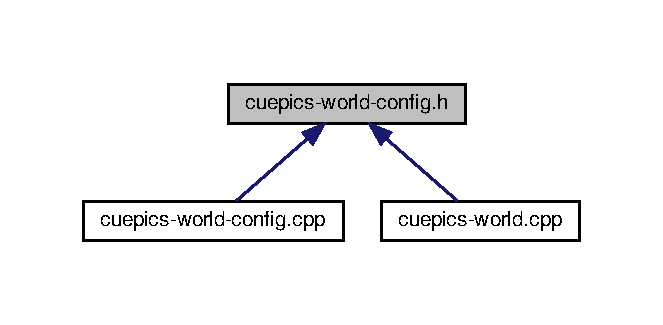
\includegraphics[width=318pt]{cuepics-world-config_8h__dep__incl}
\end{center}
\end{figure}
\subsection*{Classes}
\begin{DoxyCompactItemize}
\item 
class \textbf{ Cu\+Epics\+World\+Config}
\begin{DoxyCompactList}\small\item\em A class containing some configurations useful to several other objects. \end{DoxyCompactList}\end{DoxyCompactItemize}

\section{cuepics-\/world.cpp File Reference}
\label{cuepics-world_8cpp}\index{cuepics-\/world.\+cpp@{cuepics-\/world.\+cpp}}
{\ttfamily \#include \char`\"{}cuepics-\/world.\+h\char`\"{}}\newline
{\ttfamily \#include \char`\"{}cuepics-\/world-\/config.\+h\char`\"{}}\newline
{\ttfamily \#include $<$cumacros.\+h$>$}\newline
{\ttfamily \#include $<$regex$>$}\newline
{\ttfamily \#include $<$vector$>$}\newline
{\ttfamily \#include $<$string$>$}\newline
{\ttfamily \#include $<$stdio.\+h$>$}\newline
{\ttfamily \#include $<$stdlib.\+h$>$}\newline
{\ttfamily \#include $<$string.\+h$>$}\newline
{\ttfamily \#include $<$alarm.\+h$>$}\newline
{\ttfamily \#include $<$epics\+Time.\+h$>$}\newline
{\ttfamily \#include $<$epics\+String.\+h$>$}\newline
Include dependency graph for cuepics-\/world.cpp\+:\nopagebreak
\begin{figure}[H]
\begin{center}
\leavevmode
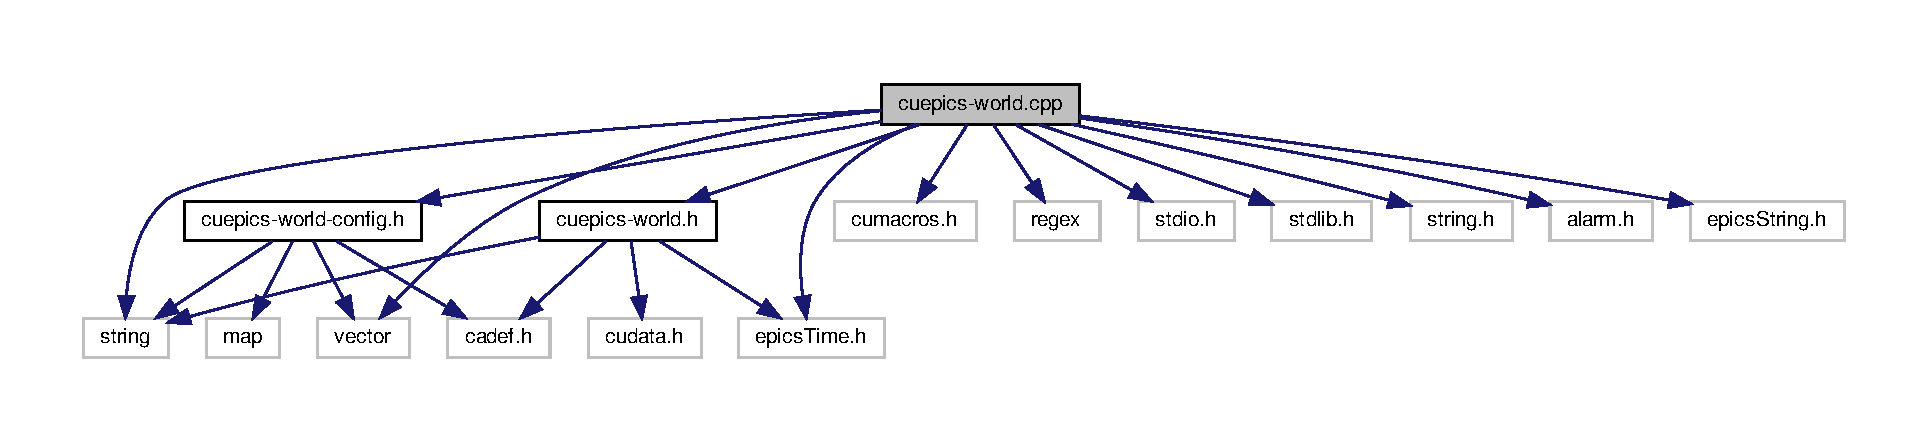
\includegraphics[width=350pt]{cuepics-world_8cpp__incl}
\end{center}
\end{figure}
\subsection*{Classes}
\begin{DoxyCompactItemize}
\item 
class \textbf{ Cu\+Epics\+World\+Private}
\end{DoxyCompactItemize}
\subsection*{Macros}
\begin{DoxyCompactItemize}
\item 
\#define \textbf{ T\+I\+M\+E\+T\+E\+X\+T\+L\+EN}~28          /$\ast$ Length of timestamp text buffer $\ast$/
\item 
\#define \textbf{ F\+M\+T\+\_\+\+T\+I\+ME}~\char`\"{}    Timestamp\+:        \%s\char`\"{}
\item 
\#define \textbf{ A\+R\+G\+S\+\_\+\+T\+I\+ME}(T)~time\+Text
\item 
\#define \textbf{ F\+M\+T\+\_\+\+S\+TS}
\item 
\#define \textbf{ A\+R\+G\+S\+\_\+\+S\+TS}(T)
\item 
\#define \textbf{ A\+R\+G\+S\+\_\+\+S\+T\+S\+\_\+\+U\+N\+S\+I\+G\+N\+ED}(T)
\item 
\#define \textbf{ F\+M\+T\+\_\+\+A\+CK}
\item 
\#define \textbf{ A\+R\+G\+S\+\_\+\+A\+CK}(T)
\item 
\#define \textbf{ F\+M\+T\+\_\+\+U\+N\+I\+TS}~\char`\"{}    Units\+:            \%s\char`\"{}
\item 
\#define \textbf{ A\+R\+G\+S\+\_\+\+U\+N\+I\+TS}(T)~((struct T $\ast$)value)-\/$>$units
\item 
\#define \textbf{ F\+M\+T\+\_\+\+P\+R\+EC}~\char`\"{}    Precision\+:        \%d\char`\"{}
\item 
\#define \textbf{ A\+R\+G\+S\+\_\+\+P\+R\+EC}(T)~((struct T $\ast$)value)-\/$>$precision
\item 
\#define \textbf{ F\+M\+T\+\_\+\+GR}(F\+MT)
\item 
\#define \textbf{ A\+R\+G\+S\+\_\+\+GR}(T,  F)
\item 
\#define \textbf{ F\+M\+T\+\_\+\+C\+T\+RL}(F\+MT)
\item 
\#define \textbf{ A\+R\+G\+S\+\_\+\+C\+T\+RL}(T,  F)
\item 
\#define \textbf{ P\+R\+N\+\_\+\+D\+B\+R\+\_\+\+S\+TS}(T)
\item 
\#define \textbf{ P\+R\+N\+\_\+\+D\+B\+R\+\_\+\+T\+I\+ME}(T)
\item 
\#define \textbf{ P\+R\+N\+\_\+\+D\+B\+R\+\_\+\+GR}(T,  F,  F\+MT)
\item 
\#define \textbf{ P\+R\+N\+\_\+\+D\+B\+R\+\_\+\+G\+R\+\_\+\+P\+R\+EC}(T,  F,  F\+MT)
\item 
\#define \textbf{ P\+R\+N\+\_\+\+D\+B\+R\+\_\+\+C\+T\+RL}(T,  F,  F\+MT)
\item 
\#define \textbf{ P\+R\+N\+\_\+\+D\+B\+R\+\_\+\+C\+T\+R\+L\+\_\+\+P\+R\+EC}(T,  F,  F\+MT)
\item 
\#define \textbf{ P\+R\+N\+\_\+\+D\+B\+R\+\_\+\+S\+T\+S\+A\+CK}(T)
\item 
\#define \textbf{ P\+R\+N\+\_\+\+D\+B\+R\+\_\+\+X\+\_\+\+E\+N\+UM}(T)
\item 
\#define \textbf{ D\+B\+R\+\_\+\+P\+R\+I\+N\+T\+\_\+\+B\+U\+F\+F\+E\+R\+\_\+\+S\+I\+ZE}
\end{DoxyCompactItemize}
\subsection*{Functions}
\begin{DoxyCompactItemize}
\item 
char $\ast$ \textbf{ dbr2str} (const void $\ast$value, unsigned type)
\item 
int \textbf{ create\+\_\+pvs} (\textbf{ Cu\+PV} $\ast$pvs, int n\+Pvs, ca\+Ch $\ast$p\+CB)
\item 
int \textbf{ connect\+\_\+pvs} (\textbf{ Cu\+PV} $\ast$pvs, int n\+Pvs)
\end{DoxyCompactItemize}
\subsection*{Variables}
\begin{DoxyCompactItemize}
\item 
char \textbf{ dbl\+Format\+Str} [30] = \char`\"{}\%g\char`\"{}
\item 
char \textbf{ time\+Format\+Str} [30] = \char`\"{}\%Y-\/\%m-\/\%d \%H\+:\%M\+:\%S.\%06f\char`\"{}
\item 
char \textbf{ field\+Separator} = \textquotesingle{} \textquotesingle{}
\item 
int \textbf{ enum\+As\+Nr} = 0
\item 
int \textbf{ char\+Arr\+As\+Str} = 0
\item 
double \textbf{ ca\+Timeout} = 1.\+0
\item 
capri \textbf{ ca\+Priority} = \textbf{ D\+E\+F\+A\+U\+L\+T\+\_\+\+C\+A\+\_\+\+P\+R\+I\+O\+R\+I\+TY}
\end{DoxyCompactItemize}


\subsection{Macro Definition Documentation}
\mbox{\label{cuepics-world_8cpp_ad3dc9bbb6870d02f047d3b9c9330d497}} 
\index{cuepics-\/world.\+cpp@{cuepics-\/world.\+cpp}!A\+R\+G\+S\+\_\+\+A\+CK@{A\+R\+G\+S\+\_\+\+A\+CK}}
\index{A\+R\+G\+S\+\_\+\+A\+CK@{A\+R\+G\+S\+\_\+\+A\+CK}!cuepics-\/world.\+cpp@{cuepics-\/world.\+cpp}}
\subsubsection{A\+R\+G\+S\+\_\+\+A\+CK}
{\footnotesize\ttfamily \#define A\+R\+G\+S\+\_\+\+A\+CK(\begin{DoxyParamCaption}\item[{}]{T }\end{DoxyParamCaption})}

{\bfseries Value\+:}
\begin{DoxyCode}
((\textcolor{keyword}{struct }T *)value)->ackt ? \textcolor{stringliteral}{"YES"} : \textcolor{stringliteral}{"NO"},   \(\backslash\)
    sevr\_to\_str\_unsigned(((\textcolor{keyword}{struct} T *)value)->acks)
\end{DoxyCode}
\mbox{\label{cuepics-world_8cpp_a8980351b4abc0732c9537704941599e9}} 
\index{cuepics-\/world.\+cpp@{cuepics-\/world.\+cpp}!A\+R\+G\+S\+\_\+\+C\+T\+RL@{A\+R\+G\+S\+\_\+\+C\+T\+RL}}
\index{A\+R\+G\+S\+\_\+\+C\+T\+RL@{A\+R\+G\+S\+\_\+\+C\+T\+RL}!cuepics-\/world.\+cpp@{cuepics-\/world.\+cpp}}
\subsubsection{A\+R\+G\+S\+\_\+\+C\+T\+RL}
{\footnotesize\ttfamily \#define A\+R\+G\+S\+\_\+\+C\+T\+RL(\begin{DoxyParamCaption}\item[{}]{T,  }\item[{}]{F }\end{DoxyParamCaption})}

{\bfseries Value\+:}
\begin{DoxyCode}
(F)((\textcolor{keyword}{struct} T *)value)->lower\_ctrl\_limit,   \(\backslash\)
    (F)((\textcolor{keyword}{struct }T *)value)->upper\_ctrl\_limit
\end{DoxyCode}
\mbox{\label{cuepics-world_8cpp_ae756576a66c8eee0f3af4872ef835f78}} 
\index{cuepics-\/world.\+cpp@{cuepics-\/world.\+cpp}!A\+R\+G\+S\+\_\+\+GR@{A\+R\+G\+S\+\_\+\+GR}}
\index{A\+R\+G\+S\+\_\+\+GR@{A\+R\+G\+S\+\_\+\+GR}!cuepics-\/world.\+cpp@{cuepics-\/world.\+cpp}}
\subsubsection{A\+R\+G\+S\+\_\+\+GR}
{\footnotesize\ttfamily \#define A\+R\+G\+S\+\_\+\+GR(\begin{DoxyParamCaption}\item[{}]{T,  }\item[{}]{F }\end{DoxyParamCaption})}

{\bfseries Value\+:}
\begin{DoxyCode}
(F)((\textcolor{keyword}{struct} T *)value)->lower\_disp\_limit,   \(\backslash\)
    (F)((\textcolor{keyword}{struct }T *)value)->upper\_disp\_limit,   \(\backslash\)
    (F)((\textcolor{keyword}{struct} T *)value)->lower\_alarm\_limit,  \(\backslash\)
    (F)((\textcolor{keyword}{struct }T *)value)->lower\_warning\_limit, \(\backslash\)
    (F)((\textcolor{keyword}{struct} T *)value)->upper\_warning\_limit, \(\backslash\)
    (F)((\textcolor{keyword}{struct }T *)value)->upper\_alarm\_limit
\end{DoxyCode}
\mbox{\label{cuepics-world_8cpp_a5991444508c9ea9a812821324d19683f}} 
\index{cuepics-\/world.\+cpp@{cuepics-\/world.\+cpp}!A\+R\+G\+S\+\_\+\+P\+R\+EC@{A\+R\+G\+S\+\_\+\+P\+R\+EC}}
\index{A\+R\+G\+S\+\_\+\+P\+R\+EC@{A\+R\+G\+S\+\_\+\+P\+R\+EC}!cuepics-\/world.\+cpp@{cuepics-\/world.\+cpp}}
\subsubsection{A\+R\+G\+S\+\_\+\+P\+R\+EC}
{\footnotesize\ttfamily \#define A\+R\+G\+S\+\_\+\+P\+R\+EC(\begin{DoxyParamCaption}\item[{}]{T }\end{DoxyParamCaption})~((struct T $\ast$)value)-\/$>$precision}

\mbox{\label{cuepics-world_8cpp_a34ec6d92f385861e90c6e975d846c0f7}} 
\index{cuepics-\/world.\+cpp@{cuepics-\/world.\+cpp}!A\+R\+G\+S\+\_\+\+S\+TS@{A\+R\+G\+S\+\_\+\+S\+TS}}
\index{A\+R\+G\+S\+\_\+\+S\+TS@{A\+R\+G\+S\+\_\+\+S\+TS}!cuepics-\/world.\+cpp@{cuepics-\/world.\+cpp}}
\subsubsection{A\+R\+G\+S\+\_\+\+S\+TS}
{\footnotesize\ttfamily \#define A\+R\+G\+S\+\_\+\+S\+TS(\begin{DoxyParamCaption}\item[{}]{T }\end{DoxyParamCaption})}

{\bfseries Value\+:}
\begin{DoxyCode}
stat_to_str(((\textcolor{keyword}{struct} T *)value)->status),   \(\backslash\)
    sevr\_to\_str(((\textcolor{keyword}{struct} T *)value)->severity)
\end{DoxyCode}
\mbox{\label{cuepics-world_8cpp_a0c3cc335f840727d94aca2b2e71902a2}} 
\index{cuepics-\/world.\+cpp@{cuepics-\/world.\+cpp}!A\+R\+G\+S\+\_\+\+S\+T\+S\+\_\+\+U\+N\+S\+I\+G\+N\+ED@{A\+R\+G\+S\+\_\+\+S\+T\+S\+\_\+\+U\+N\+S\+I\+G\+N\+ED}}
\index{A\+R\+G\+S\+\_\+\+S\+T\+S\+\_\+\+U\+N\+S\+I\+G\+N\+ED@{A\+R\+G\+S\+\_\+\+S\+T\+S\+\_\+\+U\+N\+S\+I\+G\+N\+ED}!cuepics-\/world.\+cpp@{cuepics-\/world.\+cpp}}
\subsubsection{A\+R\+G\+S\+\_\+\+S\+T\+S\+\_\+\+U\+N\+S\+I\+G\+N\+ED}
{\footnotesize\ttfamily \#define A\+R\+G\+S\+\_\+\+S\+T\+S\+\_\+\+U\+N\+S\+I\+G\+N\+ED(\begin{DoxyParamCaption}\item[{}]{T }\end{DoxyParamCaption})}

{\bfseries Value\+:}
\begin{DoxyCode}
stat_to_str_unsigned(((\textcolor{keyword}{struct} T *)value)->status),  \(\backslash\)
    sevr\_to\_str\_unsigned(((\textcolor{keyword}{struct} T *)value)->severity)
\end{DoxyCode}
\mbox{\label{cuepics-world_8cpp_af6a02f5f350dd81984b878fa094257f8}} 
\index{cuepics-\/world.\+cpp@{cuepics-\/world.\+cpp}!A\+R\+G\+S\+\_\+\+T\+I\+ME@{A\+R\+G\+S\+\_\+\+T\+I\+ME}}
\index{A\+R\+G\+S\+\_\+\+T\+I\+ME@{A\+R\+G\+S\+\_\+\+T\+I\+ME}!cuepics-\/world.\+cpp@{cuepics-\/world.\+cpp}}
\subsubsection{A\+R\+G\+S\+\_\+\+T\+I\+ME}
{\footnotesize\ttfamily \#define A\+R\+G\+S\+\_\+\+T\+I\+ME(\begin{DoxyParamCaption}\item[{}]{T }\end{DoxyParamCaption})~time\+Text}

\mbox{\label{cuepics-world_8cpp_ac2e342f50b639a6a6c24c9ce707a2029}} 
\index{cuepics-\/world.\+cpp@{cuepics-\/world.\+cpp}!A\+R\+G\+S\+\_\+\+U\+N\+I\+TS@{A\+R\+G\+S\+\_\+\+U\+N\+I\+TS}}
\index{A\+R\+G\+S\+\_\+\+U\+N\+I\+TS@{A\+R\+G\+S\+\_\+\+U\+N\+I\+TS}!cuepics-\/world.\+cpp@{cuepics-\/world.\+cpp}}
\subsubsection{A\+R\+G\+S\+\_\+\+U\+N\+I\+TS}
{\footnotesize\ttfamily \#define A\+R\+G\+S\+\_\+\+U\+N\+I\+TS(\begin{DoxyParamCaption}\item[{}]{T }\end{DoxyParamCaption})~((struct T $\ast$)value)-\/$>$units}

\mbox{\label{cuepics-world_8cpp_ab9c46c052b42b16a762fb5b52f1c3904}} 
\index{cuepics-\/world.\+cpp@{cuepics-\/world.\+cpp}!D\+B\+R\+\_\+\+P\+R\+I\+N\+T\+\_\+\+B\+U\+F\+F\+E\+R\+\_\+\+S\+I\+ZE@{D\+B\+R\+\_\+\+P\+R\+I\+N\+T\+\_\+\+B\+U\+F\+F\+E\+R\+\_\+\+S\+I\+ZE}}
\index{D\+B\+R\+\_\+\+P\+R\+I\+N\+T\+\_\+\+B\+U\+F\+F\+E\+R\+\_\+\+S\+I\+ZE@{D\+B\+R\+\_\+\+P\+R\+I\+N\+T\+\_\+\+B\+U\+F\+F\+E\+R\+\_\+\+S\+I\+ZE}!cuepics-\/world.\+cpp@{cuepics-\/world.\+cpp}}
\subsubsection{D\+B\+R\+\_\+\+P\+R\+I\+N\+T\+\_\+\+B\+U\+F\+F\+E\+R\+\_\+\+S\+I\+ZE}
{\footnotesize\ttfamily \#define D\+B\+R\+\_\+\+P\+R\+I\+N\+T\+\_\+\+B\+U\+F\+F\+E\+R\+\_\+\+S\+I\+ZE}

{\bfseries Value\+:}
\begin{DoxyCode}
50                        \textcolor{comment}{/* timestamp */}                         \(\backslash\)
    + 2 * 30                    \textcolor{comment}{/* status / Severity */}                 \(\backslash\)
    + 2 * 30                    \textcolor{comment}{/* acks / ackt */}                       \(\backslash\)
    + 20 + MAX\_UNITS\_SIZE       \textcolor{comment}{/* units */}                             \(\backslash\)
    + 30                        \textcolor{comment}{/* precision */}                         \(\backslash\)
    + 6 * 45                    \textcolor{comment}{/* graphic limits */}                    \(\backslash\)
    + 2 * 45                    \textcolor{comment}{/* control limits */}                    \(\backslash\)
    + 30 + (MAX\_ENUM\_STATES * (20 + MAX\_ENUM\_STRING\_SIZE)) \textcolor{comment}{/* enums */}  \(\backslash\)
    + 50                        \textcolor{comment}{/* just to be sure */}
\end{DoxyCode}


Referenced by dbr2str().

\mbox{\label{cuepics-world_8cpp_a535506b14ed6cd00891461bae5908cb3}} 
\index{cuepics-\/world.\+cpp@{cuepics-\/world.\+cpp}!F\+M\+T\+\_\+\+A\+CK@{F\+M\+T\+\_\+\+A\+CK}}
\index{F\+M\+T\+\_\+\+A\+CK@{F\+M\+T\+\_\+\+A\+CK}!cuepics-\/world.\+cpp@{cuepics-\/world.\+cpp}}
\subsubsection{F\+M\+T\+\_\+\+A\+CK}
{\footnotesize\ttfamily \#define F\+M\+T\+\_\+\+A\+CK}

{\bfseries Value\+:}
\begin{DoxyCode}
\textcolor{stringliteral}{"    Ack transient?:   %s\(\backslash\)n"}                \(\backslash\)
    \textcolor{stringliteral}{"    Ack severity:     %s"}
\end{DoxyCode}
\mbox{\label{cuepics-world_8cpp_a9ec448c630a99dd83240a72c4c8f6b76}} 
\index{cuepics-\/world.\+cpp@{cuepics-\/world.\+cpp}!F\+M\+T\+\_\+\+C\+T\+RL@{F\+M\+T\+\_\+\+C\+T\+RL}}
\index{F\+M\+T\+\_\+\+C\+T\+RL@{F\+M\+T\+\_\+\+C\+T\+RL}!cuepics-\/world.\+cpp@{cuepics-\/world.\+cpp}}
\subsubsection{F\+M\+T\+\_\+\+C\+T\+RL}
{\footnotesize\ttfamily \#define F\+M\+T\+\_\+\+C\+T\+RL(\begin{DoxyParamCaption}\item[{}]{F\+MT }\end{DoxyParamCaption})}

{\bfseries Value\+:}
\begin{DoxyCode}
\textcolor{stringliteral}{"    Lo ctrl limit:    "} #FMT \textcolor{stringliteral}{"\(\backslash\)n"}          \(\backslash\)
    \textcolor{stringliteral}{"    Hi ctrl limit:    "} #FMT
\end{DoxyCode}
\mbox{\label{cuepics-world_8cpp_a198c5670c00cdce095fcb90c7a9dc502}} 
\index{cuepics-\/world.\+cpp@{cuepics-\/world.\+cpp}!F\+M\+T\+\_\+\+GR@{F\+M\+T\+\_\+\+GR}}
\index{F\+M\+T\+\_\+\+GR@{F\+M\+T\+\_\+\+GR}!cuepics-\/world.\+cpp@{cuepics-\/world.\+cpp}}
\subsubsection{F\+M\+T\+\_\+\+GR}
{\footnotesize\ttfamily \#define F\+M\+T\+\_\+\+GR(\begin{DoxyParamCaption}\item[{}]{F\+MT }\end{DoxyParamCaption})}

{\bfseries Value\+:}
\begin{DoxyCode}
\textcolor{stringliteral}{"    Lo disp limit:    "} #FMT \textcolor{stringliteral}{"\(\backslash\)n"}          \(\backslash\)
    \textcolor{stringliteral}{"    Hi disp limit:    "} #FMT \textcolor{stringliteral}{"\(\backslash\)n"}          \(\backslash\)
    \textcolor{stringliteral}{"    Lo alarm limit:   "} #FMT \textcolor{stringliteral}{"\(\backslash\)n"}          \(\backslash\)
    \textcolor{stringliteral}{"    Lo warn limit:    "} #FMT \textcolor{stringliteral}{"\(\backslash\)n"}          \(\backslash\)
    \textcolor{stringliteral}{"    Hi warn limit:    "} #FMT \textcolor{stringliteral}{"\(\backslash\)n"}          \(\backslash\)
    \textcolor{stringliteral}{"    Hi alarm limit:   "} #FMT
\end{DoxyCode}
\mbox{\label{cuepics-world_8cpp_a8629eb39aeb7a9e156c6a06abd51accf}} 
\index{cuepics-\/world.\+cpp@{cuepics-\/world.\+cpp}!F\+M\+T\+\_\+\+P\+R\+EC@{F\+M\+T\+\_\+\+P\+R\+EC}}
\index{F\+M\+T\+\_\+\+P\+R\+EC@{F\+M\+T\+\_\+\+P\+R\+EC}!cuepics-\/world.\+cpp@{cuepics-\/world.\+cpp}}
\subsubsection{F\+M\+T\+\_\+\+P\+R\+EC}
{\footnotesize\ttfamily \#define F\+M\+T\+\_\+\+P\+R\+EC~\char`\"{}    Precision\+:        \%d\char`\"{}}

\mbox{\label{cuepics-world_8cpp_a47d7a4b59d8262932b8361c24094af19}} 
\index{cuepics-\/world.\+cpp@{cuepics-\/world.\+cpp}!F\+M\+T\+\_\+\+S\+TS@{F\+M\+T\+\_\+\+S\+TS}}
\index{F\+M\+T\+\_\+\+S\+TS@{F\+M\+T\+\_\+\+S\+TS}!cuepics-\/world.\+cpp@{cuepics-\/world.\+cpp}}
\subsubsection{F\+M\+T\+\_\+\+S\+TS}
{\footnotesize\ttfamily \#define F\+M\+T\+\_\+\+S\+TS}

{\bfseries Value\+:}
\begin{DoxyCode}
\textcolor{stringliteral}{"    Status:           %s\(\backslash\)n"}                \(\backslash\)
    \textcolor{stringliteral}{"    Severity:         %s"}
\end{DoxyCode}
\mbox{\label{cuepics-world_8cpp_a6c3ba388a488ad2cf5c9fecad527de66}} 
\index{cuepics-\/world.\+cpp@{cuepics-\/world.\+cpp}!F\+M\+T\+\_\+\+T\+I\+ME@{F\+M\+T\+\_\+\+T\+I\+ME}}
\index{F\+M\+T\+\_\+\+T\+I\+ME@{F\+M\+T\+\_\+\+T\+I\+ME}!cuepics-\/world.\+cpp@{cuepics-\/world.\+cpp}}
\subsubsection{F\+M\+T\+\_\+\+T\+I\+ME}
{\footnotesize\ttfamily \#define F\+M\+T\+\_\+\+T\+I\+ME~\char`\"{}    Timestamp\+:        \%s\char`\"{}}

\mbox{\label{cuepics-world_8cpp_a3a614b78bc0be0167a64e695d8d03601}} 
\index{cuepics-\/world.\+cpp@{cuepics-\/world.\+cpp}!F\+M\+T\+\_\+\+U\+N\+I\+TS@{F\+M\+T\+\_\+\+U\+N\+I\+TS}}
\index{F\+M\+T\+\_\+\+U\+N\+I\+TS@{F\+M\+T\+\_\+\+U\+N\+I\+TS}!cuepics-\/world.\+cpp@{cuepics-\/world.\+cpp}}
\subsubsection{F\+M\+T\+\_\+\+U\+N\+I\+TS}
{\footnotesize\ttfamily \#define F\+M\+T\+\_\+\+U\+N\+I\+TS~\char`\"{}    Units\+:            \%s\char`\"{}}

\mbox{\label{cuepics-world_8cpp_a09b5c761e5a4c841ee2ff2c1b425d87d}} 
\index{cuepics-\/world.\+cpp@{cuepics-\/world.\+cpp}!P\+R\+N\+\_\+\+D\+B\+R\+\_\+\+C\+T\+RL@{P\+R\+N\+\_\+\+D\+B\+R\+\_\+\+C\+T\+RL}}
\index{P\+R\+N\+\_\+\+D\+B\+R\+\_\+\+C\+T\+RL@{P\+R\+N\+\_\+\+D\+B\+R\+\_\+\+C\+T\+RL}!cuepics-\/world.\+cpp@{cuepics-\/world.\+cpp}}
\subsubsection{P\+R\+N\+\_\+\+D\+B\+R\+\_\+\+C\+T\+RL}
{\footnotesize\ttfamily \#define P\+R\+N\+\_\+\+D\+B\+R\+\_\+\+C\+T\+RL(\begin{DoxyParamCaption}\item[{}]{T,  }\item[{}]{F,  }\item[{}]{F\+MT }\end{DoxyParamCaption})}

{\bfseries Value\+:}
\begin{DoxyCode}
sprintf(str,                                                                \(\backslash\)
    FMT_STS \textcolor{stringliteral}{"\(\backslash\)n"} FMT_UNITS \textcolor{stringliteral}{"\(\backslash\)n"} FMT_GR(FMT) \textcolor{stringliteral}{"\(\backslash\)n"} FMT_CTRL(FMT),         \(\backslash\)
    ARGS_STS(T), ARGS_UNITS(T), ARGS_GR(T,F),    ARGS_CTRL(T,F))
\end{DoxyCode}


Referenced by dbr2str().

\mbox{\label{cuepics-world_8cpp_a1416ed646e86c2d9b66a586d3af7a6e7}} 
\index{cuepics-\/world.\+cpp@{cuepics-\/world.\+cpp}!P\+R\+N\+\_\+\+D\+B\+R\+\_\+\+C\+T\+R\+L\+\_\+\+P\+R\+EC@{P\+R\+N\+\_\+\+D\+B\+R\+\_\+\+C\+T\+R\+L\+\_\+\+P\+R\+EC}}
\index{P\+R\+N\+\_\+\+D\+B\+R\+\_\+\+C\+T\+R\+L\+\_\+\+P\+R\+EC@{P\+R\+N\+\_\+\+D\+B\+R\+\_\+\+C\+T\+R\+L\+\_\+\+P\+R\+EC}!cuepics-\/world.\+cpp@{cuepics-\/world.\+cpp}}
\subsubsection{P\+R\+N\+\_\+\+D\+B\+R\+\_\+\+C\+T\+R\+L\+\_\+\+P\+R\+EC}
{\footnotesize\ttfamily \#define P\+R\+N\+\_\+\+D\+B\+R\+\_\+\+C\+T\+R\+L\+\_\+\+P\+R\+EC(\begin{DoxyParamCaption}\item[{}]{T,  }\item[{}]{F,  }\item[{}]{F\+MT }\end{DoxyParamCaption})}

{\bfseries Value\+:}
\begin{DoxyCode}
sprintf(str,                                                                        \(\backslash\)
    FMT_STS \textcolor{stringliteral}{"\(\backslash\)n"} FMT_UNITS \textcolor{stringliteral}{"\(\backslash\)n"} FMT_PREC \textcolor{stringliteral}{"\(\backslash\)n"} FMT_GR(FMT) \textcolor{stringliteral}{"\(\backslash\)n"} FMT_CTRL(FMT),   \(\backslash\)
    ARGS_STS(T), ARGS_UNITS(T), ARGS_PREC(T), ARGS_GR(T,F),    ARGS_CTRL(T,F))
\end{DoxyCode}


Referenced by dbr2str().

\mbox{\label{cuepics-world_8cpp_a43d963aa4a72306b9eb999354dbea088}} 
\index{cuepics-\/world.\+cpp@{cuepics-\/world.\+cpp}!P\+R\+N\+\_\+\+D\+B\+R\+\_\+\+GR@{P\+R\+N\+\_\+\+D\+B\+R\+\_\+\+GR}}
\index{P\+R\+N\+\_\+\+D\+B\+R\+\_\+\+GR@{P\+R\+N\+\_\+\+D\+B\+R\+\_\+\+GR}!cuepics-\/world.\+cpp@{cuepics-\/world.\+cpp}}
\subsubsection{P\+R\+N\+\_\+\+D\+B\+R\+\_\+\+GR}
{\footnotesize\ttfamily \#define P\+R\+N\+\_\+\+D\+B\+R\+\_\+\+GR(\begin{DoxyParamCaption}\item[{}]{T,  }\item[{}]{F,  }\item[{}]{F\+MT }\end{DoxyParamCaption})}

{\bfseries Value\+:}
\begin{DoxyCode}
sprintf(str,                                        \(\backslash\)
    FMT_STS \textcolor{stringliteral}{"\(\backslash\)n"} FMT_UNITS \textcolor{stringliteral}{"\(\backslash\)n"} FMT_GR(FMT),    \(\backslash\)
    ARGS_STS(T), ARGS_UNITS(T), ARGS_GR(T,F))
\end{DoxyCode}


Referenced by dbr2str().

\mbox{\label{cuepics-world_8cpp_ae58f9da42d2cf10ce60d46239338f857}} 
\index{cuepics-\/world.\+cpp@{cuepics-\/world.\+cpp}!P\+R\+N\+\_\+\+D\+B\+R\+\_\+\+G\+R\+\_\+\+P\+R\+EC@{P\+R\+N\+\_\+\+D\+B\+R\+\_\+\+G\+R\+\_\+\+P\+R\+EC}}
\index{P\+R\+N\+\_\+\+D\+B\+R\+\_\+\+G\+R\+\_\+\+P\+R\+EC@{P\+R\+N\+\_\+\+D\+B\+R\+\_\+\+G\+R\+\_\+\+P\+R\+EC}!cuepics-\/world.\+cpp@{cuepics-\/world.\+cpp}}
\subsubsection{P\+R\+N\+\_\+\+D\+B\+R\+\_\+\+G\+R\+\_\+\+P\+R\+EC}
{\footnotesize\ttfamily \#define P\+R\+N\+\_\+\+D\+B\+R\+\_\+\+G\+R\+\_\+\+P\+R\+EC(\begin{DoxyParamCaption}\item[{}]{T,  }\item[{}]{F,  }\item[{}]{F\+MT }\end{DoxyParamCaption})}

{\bfseries Value\+:}
\begin{DoxyCode}
sprintf(str,                                                        \(\backslash\)
    FMT_STS \textcolor{stringliteral}{"\(\backslash\)n"} FMT_UNITS \textcolor{stringliteral}{"\(\backslash\)n"} FMT_PREC \textcolor{stringliteral}{"\(\backslash\)n"} FMT_GR(FMT),      \(\backslash\)
    ARGS_STS(T), ARGS_UNITS(T), ARGS_PREC(T), ARGS_GR(T,F))
\end{DoxyCode}


Referenced by dbr2str().

\mbox{\label{cuepics-world_8cpp_a02f221ce80ed853021c08f24325a0317}} 
\index{cuepics-\/world.\+cpp@{cuepics-\/world.\+cpp}!P\+R\+N\+\_\+\+D\+B\+R\+\_\+\+S\+TS@{P\+R\+N\+\_\+\+D\+B\+R\+\_\+\+S\+TS}}
\index{P\+R\+N\+\_\+\+D\+B\+R\+\_\+\+S\+TS@{P\+R\+N\+\_\+\+D\+B\+R\+\_\+\+S\+TS}!cuepics-\/world.\+cpp@{cuepics-\/world.\+cpp}}
\subsubsection{P\+R\+N\+\_\+\+D\+B\+R\+\_\+\+S\+TS}
{\footnotesize\ttfamily \#define P\+R\+N\+\_\+\+D\+B\+R\+\_\+\+S\+TS(\begin{DoxyParamCaption}\item[{}]{T }\end{DoxyParamCaption})}

{\bfseries Value\+:}
\begin{DoxyCode}
sprintf(str,                                \(\backslash\)
    FMT_STS,                            \(\backslash\)
    ARGS_STS(T))
\end{DoxyCode}


Referenced by dbr2str().

\mbox{\label{cuepics-world_8cpp_aa8af4ab3587a067d7fb5882feb11a9ea}} 
\index{cuepics-\/world.\+cpp@{cuepics-\/world.\+cpp}!P\+R\+N\+\_\+\+D\+B\+R\+\_\+\+S\+T\+S\+A\+CK@{P\+R\+N\+\_\+\+D\+B\+R\+\_\+\+S\+T\+S\+A\+CK}}
\index{P\+R\+N\+\_\+\+D\+B\+R\+\_\+\+S\+T\+S\+A\+CK@{P\+R\+N\+\_\+\+D\+B\+R\+\_\+\+S\+T\+S\+A\+CK}!cuepics-\/world.\+cpp@{cuepics-\/world.\+cpp}}
\subsubsection{P\+R\+N\+\_\+\+D\+B\+R\+\_\+\+S\+T\+S\+A\+CK}
{\footnotesize\ttfamily \#define P\+R\+N\+\_\+\+D\+B\+R\+\_\+\+S\+T\+S\+A\+CK(\begin{DoxyParamCaption}\item[{}]{T }\end{DoxyParamCaption})}

{\bfseries Value\+:}
\begin{DoxyCode}
sprintf(str,                                \(\backslash\)
    FMT_STS \textcolor{stringliteral}{"\(\backslash\)n"} FMT_ACK,               \(\backslash\)
    ARGS_STS_UNSIGNED(T), ARGS_ACK(T))
\end{DoxyCode}


Referenced by dbr2str().

\mbox{\label{cuepics-world_8cpp_a5571c3df911af191bda65996e71523c9}} 
\index{cuepics-\/world.\+cpp@{cuepics-\/world.\+cpp}!P\+R\+N\+\_\+\+D\+B\+R\+\_\+\+T\+I\+ME@{P\+R\+N\+\_\+\+D\+B\+R\+\_\+\+T\+I\+ME}}
\index{P\+R\+N\+\_\+\+D\+B\+R\+\_\+\+T\+I\+ME@{P\+R\+N\+\_\+\+D\+B\+R\+\_\+\+T\+I\+ME}!cuepics-\/world.\+cpp@{cuepics-\/world.\+cpp}}
\subsubsection{P\+R\+N\+\_\+\+D\+B\+R\+\_\+\+T\+I\+ME}
{\footnotesize\ttfamily \#define P\+R\+N\+\_\+\+D\+B\+R\+\_\+\+T\+I\+ME(\begin{DoxyParamCaption}\item[{}]{T }\end{DoxyParamCaption})}

{\bfseries Value\+:}
\begin{DoxyCode}
epicsTimeToStrftime(timeText, TIMETEXTLEN, timeFormatStr,   \(\backslash\)
    &(((\textcolor{keyword}{struct} T *)value)->stamp));         \(\backslash\)
    sprintf(str,                                                \(\backslash\)
    FMT_TIME \textcolor{stringliteral}{"\(\backslash\)n"} FMT_STS,                              \(\backslash\)
    ARGS_TIME(T), ARGS_STS(T))
\end{DoxyCode}


Referenced by dbr2str().

\mbox{\label{cuepics-world_8cpp_aabf7e2ac7e330a82c65d5bf0e9be8f2b}} 
\index{cuepics-\/world.\+cpp@{cuepics-\/world.\+cpp}!P\+R\+N\+\_\+\+D\+B\+R\+\_\+\+X\+\_\+\+E\+N\+UM@{P\+R\+N\+\_\+\+D\+B\+R\+\_\+\+X\+\_\+\+E\+N\+UM}}
\index{P\+R\+N\+\_\+\+D\+B\+R\+\_\+\+X\+\_\+\+E\+N\+UM@{P\+R\+N\+\_\+\+D\+B\+R\+\_\+\+X\+\_\+\+E\+N\+UM}!cuepics-\/world.\+cpp@{cuepics-\/world.\+cpp}}
\subsubsection{P\+R\+N\+\_\+\+D\+B\+R\+\_\+\+X\+\_\+\+E\+N\+UM}
{\footnotesize\ttfamily \#define P\+R\+N\+\_\+\+D\+B\+R\+\_\+\+X\+\_\+\+E\+N\+UM(\begin{DoxyParamCaption}\item[{}]{T }\end{DoxyParamCaption})}

{\bfseries Value\+:}
\begin{DoxyCode}
n = ((\textcolor{keyword}{struct }T *)value)->no\_str;                    \(\backslash\)
    PRN\_DBR\_STS(T);                                     \(\backslash\)
    sprintf(str+strlen(str),                            \(\backslash\)
    \textcolor{stringliteral}{"\(\backslash\)n    Enums:            (%2d)"}, n);    \(\backslash\)
    for (i=0; i<n; i++)                                 \(\backslash\)
    sprintf(str+strlen(str),                        \(\backslash\)
    \textcolor{stringliteral}{"\(\backslash\)n                      [%2d] %s"}, i,  \(\backslash\)
    ((\textcolor{keyword}{struct} T *)value)->strs[i]);
\end{DoxyCode}


Referenced by dbr2str().

\mbox{\label{cuepics-world_8cpp_a995e052e2e4953cee4eca69051f17801}} 
\index{cuepics-\/world.\+cpp@{cuepics-\/world.\+cpp}!T\+I\+M\+E\+T\+E\+X\+T\+L\+EN@{T\+I\+M\+E\+T\+E\+X\+T\+L\+EN}}
\index{T\+I\+M\+E\+T\+E\+X\+T\+L\+EN@{T\+I\+M\+E\+T\+E\+X\+T\+L\+EN}!cuepics-\/world.\+cpp@{cuepics-\/world.\+cpp}}
\subsubsection{T\+I\+M\+E\+T\+E\+X\+T\+L\+EN}
{\footnotesize\ttfamily \#define T\+I\+M\+E\+T\+E\+X\+T\+L\+EN~28          /$\ast$ Length of timestamp text buffer $\ast$/}



Referenced by dbr2str(), and Cu\+Epics\+World\+::put\+Timestamp().



\subsection{Function Documentation}
\mbox{\label{cuepics-world_8cpp_a9b5b6025321a6802e5c0e16fc5f7ce9a}} 
\index{cuepics-\/world.\+cpp@{cuepics-\/world.\+cpp}!connect\+\_\+pvs@{connect\+\_\+pvs}}
\index{connect\+\_\+pvs@{connect\+\_\+pvs}!cuepics-\/world.\+cpp@{cuepics-\/world.\+cpp}}
\subsubsection{connect\+\_\+pvs()}
{\footnotesize\ttfamily int connect\+\_\+pvs (\begin{DoxyParamCaption}\item[{\textbf{ Cu\+PV} $\ast$}]{pvs,  }\item[{int}]{n\+Pvs }\end{DoxyParamCaption})}



References ca\+Timeout, and create\+\_\+pvs().

\mbox{\label{cuepics-world_8cpp_a0e2d4c91a34468490cbfccf013e05ea5}} 
\index{cuepics-\/world.\+cpp@{cuepics-\/world.\+cpp}!create\+\_\+pvs@{create\+\_\+pvs}}
\index{create\+\_\+pvs@{create\+\_\+pvs}!cuepics-\/world.\+cpp@{cuepics-\/world.\+cpp}}
\subsubsection{create\+\_\+pvs()}
{\footnotesize\ttfamily int create\+\_\+pvs (\begin{DoxyParamCaption}\item[{\textbf{ Cu\+PV} $\ast$}]{pvs,  }\item[{int}]{n\+Pvs,  }\item[{ca\+Ch $\ast$}]{p\+CB }\end{DoxyParamCaption})}



References ca\+Priority, and Cu\+P\+V\+::status.



Referenced by connect\+\_\+pvs(), and Cu\+Monitor\+Activity\+::init().

\mbox{\label{cuepics-world_8cpp_a703b41b0f7b2221eff13d827ae0ab9b3}} 
\index{cuepics-\/world.\+cpp@{cuepics-\/world.\+cpp}!dbr2str@{dbr2str}}
\index{dbr2str@{dbr2str}!cuepics-\/world.\+cpp@{cuepics-\/world.\+cpp}}
\subsubsection{dbr2str()}
{\footnotesize\ttfamily char$\ast$ dbr2str (\begin{DoxyParamCaption}\item[{const void $\ast$}]{value,  }\item[{unsigned}]{type }\end{DoxyParamCaption})}



References D\+B\+R\+\_\+\+P\+R\+I\+N\+T\+\_\+\+B\+U\+F\+F\+E\+R\+\_\+\+S\+I\+ZE, P\+R\+N\+\_\+\+D\+B\+R\+\_\+\+C\+T\+RL, P\+R\+N\+\_\+\+D\+B\+R\+\_\+\+C\+T\+R\+L\+\_\+\+P\+R\+EC, P\+R\+N\+\_\+\+D\+B\+R\+\_\+\+GR, P\+R\+N\+\_\+\+D\+B\+R\+\_\+\+G\+R\+\_\+\+P\+R\+EC, P\+R\+N\+\_\+\+D\+B\+R\+\_\+\+S\+TS, P\+R\+N\+\_\+\+D\+B\+R\+\_\+\+S\+T\+S\+A\+CK, P\+R\+N\+\_\+\+D\+B\+R\+\_\+\+T\+I\+ME, P\+R\+N\+\_\+\+D\+B\+R\+\_\+\+X\+\_\+\+E\+N\+UM, and T\+I\+M\+E\+T\+E\+X\+T\+L\+EN.



\subsection{Variable Documentation}
\mbox{\label{cuepics-world_8cpp_acd49e1150b00929469c7ee6045c317bf}} 
\index{cuepics-\/world.\+cpp@{cuepics-\/world.\+cpp}!ca\+Priority@{ca\+Priority}}
\index{ca\+Priority@{ca\+Priority}!cuepics-\/world.\+cpp@{cuepics-\/world.\+cpp}}
\subsubsection{ca\+Priority}
{\footnotesize\ttfamily capri ca\+Priority = \textbf{ D\+E\+F\+A\+U\+L\+T\+\_\+\+C\+A\+\_\+\+P\+R\+I\+O\+R\+I\+TY}}



Referenced by create\+\_\+pvs().

\mbox{\label{cuepics-world_8cpp_a849d8602b082fe2275cc6c6c7ad40a36}} 
\index{cuepics-\/world.\+cpp@{cuepics-\/world.\+cpp}!ca\+Timeout@{ca\+Timeout}}
\index{ca\+Timeout@{ca\+Timeout}!cuepics-\/world.\+cpp@{cuepics-\/world.\+cpp}}
\subsubsection{ca\+Timeout}
{\footnotesize\ttfamily double ca\+Timeout = 1.\+0}



Referenced by connect\+\_\+pvs(), and Cu\+Monitor\+Activity\+::init().

\mbox{\label{cuepics-world_8cpp_ab815500b3a67737b1515e93ead71be9a}} 
\index{cuepics-\/world.\+cpp@{cuepics-\/world.\+cpp}!char\+Arr\+As\+Str@{char\+Arr\+As\+Str}}
\index{char\+Arr\+As\+Str@{char\+Arr\+As\+Str}!cuepics-\/world.\+cpp@{cuepics-\/world.\+cpp}}
\subsubsection{char\+Arr\+As\+Str}
{\footnotesize\ttfamily int char\+Arr\+As\+Str = 0}

\mbox{\label{cuepics-world_8cpp_acecde06e62d65b0846442140b3f0089f}} 
\index{cuepics-\/world.\+cpp@{cuepics-\/world.\+cpp}!dbl\+Format\+Str@{dbl\+Format\+Str}}
\index{dbl\+Format\+Str@{dbl\+Format\+Str}!cuepics-\/world.\+cpp@{cuepics-\/world.\+cpp}}
\subsubsection{dbl\+Format\+Str}
{\footnotesize\ttfamily char dbl\+Format\+Str[30] = \char`\"{}\%g\char`\"{}}

\mbox{\label{cuepics-world_8cpp_ac5d1502aca61767572e2b377375668b3}} 
\index{cuepics-\/world.\+cpp@{cuepics-\/world.\+cpp}!enum\+As\+Nr@{enum\+As\+Nr}}
\index{enum\+As\+Nr@{enum\+As\+Nr}!cuepics-\/world.\+cpp@{cuepics-\/world.\+cpp}}
\subsubsection{enum\+As\+Nr}
{\footnotesize\ttfamily int enum\+As\+Nr = 0}



Referenced by Cu\+Monitor\+Activity\+::connection\+\_\+handler().

\mbox{\label{cuepics-world_8cpp_a95466c19d4d0e1ad87c6a0852119dc6b}} 
\index{cuepics-\/world.\+cpp@{cuepics-\/world.\+cpp}!field\+Separator@{field\+Separator}}
\index{field\+Separator@{field\+Separator}!cuepics-\/world.\+cpp@{cuepics-\/world.\+cpp}}
\subsubsection{field\+Separator}
{\footnotesize\ttfamily char field\+Separator = \textquotesingle{} \textquotesingle{}}

\mbox{\label{cuepics-world_8cpp_aef64c841c7d11f7342513f8315fc24de}} 
\index{cuepics-\/world.\+cpp@{cuepics-\/world.\+cpp}!time\+Format\+Str@{time\+Format\+Str}}
\index{time\+Format\+Str@{time\+Format\+Str}!cuepics-\/world.\+cpp@{cuepics-\/world.\+cpp}}
\subsubsection{time\+Format\+Str}
{\footnotesize\ttfamily char time\+Format\+Str[30] = \char`\"{}\%Y-\/\%m-\/\%d \%H\+:\%M\+:\%S.\%06f\char`\"{}}


\section{cuepics-\/world.h File Reference}
\label{cuepics-world_8h}\index{cuepics-\/world.\+h@{cuepics-\/world.\+h}}
{\ttfamily \#include $<$string$>$}\newline
{\ttfamily \#include $<$cudata.\+h$>$}\newline
{\ttfamily \#include $<$cadef.\+h$>$}\newline
{\ttfamily \#include $<$epics\+Time.\+h$>$}\newline
Include dependency graph for cuepics-\/world.h\+:\nopagebreak
\begin{figure}[H]
\begin{center}
\leavevmode
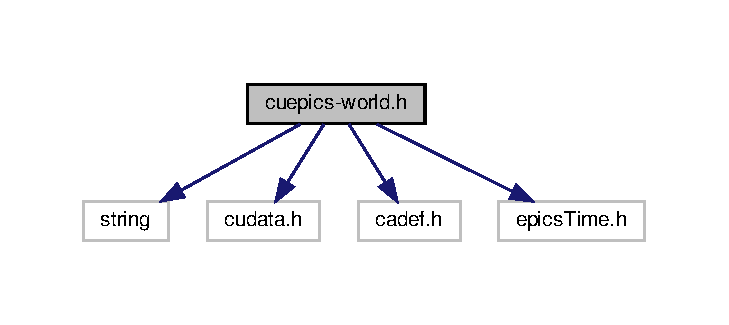
\includegraphics[width=350pt]{cuepics-world_8h__incl}
\end{center}
\end{figure}
This graph shows which files directly or indirectly include this file\+:\nopagebreak
\begin{figure}[H]
\begin{center}
\leavevmode
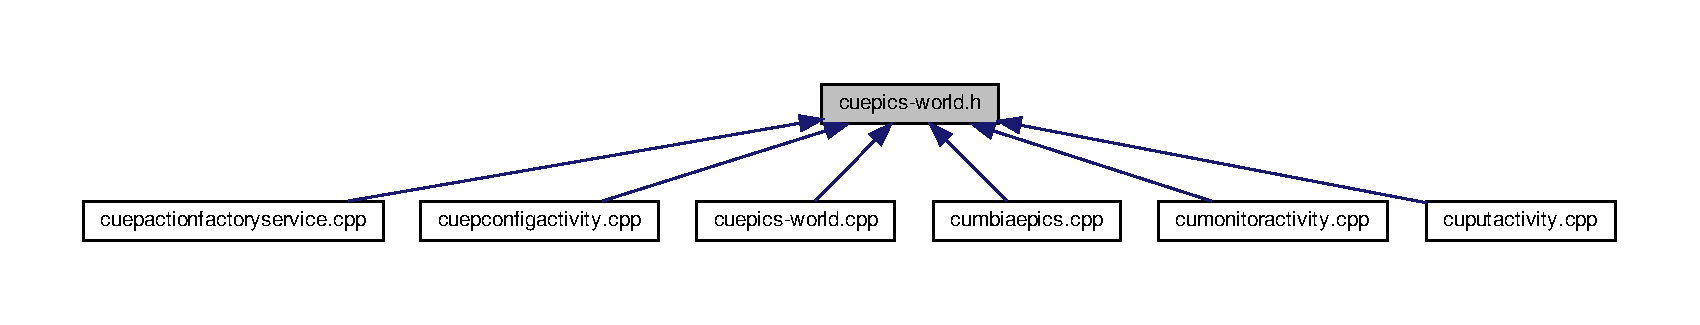
\includegraphics[width=350pt]{cuepics-world_8h__dep__incl}
\end{center}
\end{figure}
\subsection*{Classes}
\begin{DoxyCompactItemize}
\item 
struct \textbf{ Cu\+PV}
\item 
class \textbf{ Cu\+Epics\+World}
\end{DoxyCompactItemize}
\subsection*{Macros}
\begin{DoxyCompactItemize}
\item 
\#define \textbf{ stat\+\_\+to\+\_\+str}(stat)
\item 
\#define \textbf{ sevr\+\_\+to\+\_\+str}(stat)
\item 
\#define \textbf{ stat\+\_\+to\+\_\+str\+\_\+unsigned}(stat)
\item 
\#define \textbf{ sevr\+\_\+to\+\_\+str\+\_\+unsigned}(stat)
\item 
\#define \textbf{ D\+E\+F\+A\+U\+L\+T\+\_\+\+C\+A\+\_\+\+P\+R\+I\+O\+R\+I\+TY}~0  /$\ast$ Default CA priority $\ast$/
\item 
\#define \textbf{ D\+E\+F\+A\+U\+L\+T\+\_\+\+C\+A\+\_\+\+T\+I\+M\+E\+O\+UT}~1.\+0     /$\ast$ Default CA timeout $\ast$/
\end{DoxyCompactItemize}
\subsection*{Functions}
\begin{DoxyCompactItemize}
\item 
char $\ast$ \textbf{ val2str} (const void $\ast$v, unsigned type, int index)
\item 
char $\ast$ \textbf{ dbr2str} (const void $\ast$value, unsigned type)
\item 
void \textbf{ print\+\_\+time\+\_\+val\+\_\+sts} (\textbf{ Cu\+PV} $\ast$\textbf{ Cu\+PV}, unsigned long req\+Elems)
\item 
int \textbf{ create\+\_\+pvs} (\textbf{ Cu\+PV} $\ast$pvs, int n\+Pvs, ca\+Ch $\ast$p\+CB)
\item 
int \textbf{ connect\+\_\+pvs} (\textbf{ Cu\+PV} $\ast$pvs, int n\+Pvs)
\end{DoxyCompactItemize}
\subsection*{Variables}
\begin{DoxyCompactItemize}
\item 
int \textbf{ ts\+Src\+Server}
\item 
int \textbf{ ts\+Src\+Client}
\item 
int \textbf{ enum\+As\+Nr}
\item 
int \textbf{ char\+Arr\+As\+Str}
\item 
double \textbf{ ca\+Timeout}
\item 
char \textbf{ dbl\+Format\+Str} [$\,$]
\item 
char \textbf{ field\+Separator}
\item 
capri \textbf{ ca\+Priority}
\end{DoxyCompactItemize}


\subsection{Macro Definition Documentation}
\mbox{\label{cuepics-world_8h_a6d8de8e70685f0bb36fb3fb37d17fc5c}} 
\index{cuepics-\/world.\+h@{cuepics-\/world.\+h}!D\+E\+F\+A\+U\+L\+T\+\_\+\+C\+A\+\_\+\+P\+R\+I\+O\+R\+I\+TY@{D\+E\+F\+A\+U\+L\+T\+\_\+\+C\+A\+\_\+\+P\+R\+I\+O\+R\+I\+TY}}
\index{D\+E\+F\+A\+U\+L\+T\+\_\+\+C\+A\+\_\+\+P\+R\+I\+O\+R\+I\+TY@{D\+E\+F\+A\+U\+L\+T\+\_\+\+C\+A\+\_\+\+P\+R\+I\+O\+R\+I\+TY}!cuepics-\/world.\+h@{cuepics-\/world.\+h}}
\subsubsection{D\+E\+F\+A\+U\+L\+T\+\_\+\+C\+A\+\_\+\+P\+R\+I\+O\+R\+I\+TY}
{\footnotesize\ttfamily \#define D\+E\+F\+A\+U\+L\+T\+\_\+\+C\+A\+\_\+\+P\+R\+I\+O\+R\+I\+TY~0  /$\ast$ Default CA priority $\ast$/}

\mbox{\label{cuepics-world_8h_af16d153c96320f645bb69bff1c124458}} 
\index{cuepics-\/world.\+h@{cuepics-\/world.\+h}!D\+E\+F\+A\+U\+L\+T\+\_\+\+C\+A\+\_\+\+T\+I\+M\+E\+O\+UT@{D\+E\+F\+A\+U\+L\+T\+\_\+\+C\+A\+\_\+\+T\+I\+M\+E\+O\+UT}}
\index{D\+E\+F\+A\+U\+L\+T\+\_\+\+C\+A\+\_\+\+T\+I\+M\+E\+O\+UT@{D\+E\+F\+A\+U\+L\+T\+\_\+\+C\+A\+\_\+\+T\+I\+M\+E\+O\+UT}!cuepics-\/world.\+h@{cuepics-\/world.\+h}}
\subsubsection{D\+E\+F\+A\+U\+L\+T\+\_\+\+C\+A\+\_\+\+T\+I\+M\+E\+O\+UT}
{\footnotesize\ttfamily \#define D\+E\+F\+A\+U\+L\+T\+\_\+\+C\+A\+\_\+\+T\+I\+M\+E\+O\+UT~1.\+0     /$\ast$ Default CA timeout $\ast$/}



Referenced by Cu\+Monitor\+Activity\+::init().

\mbox{\label{cuepics-world_8h_ab950f17fbdedaa1c6d23ed63b4e38466}} 
\index{cuepics-\/world.\+h@{cuepics-\/world.\+h}!sevr\+\_\+to\+\_\+str@{sevr\+\_\+to\+\_\+str}}
\index{sevr\+\_\+to\+\_\+str@{sevr\+\_\+to\+\_\+str}!cuepics-\/world.\+h@{cuepics-\/world.\+h}}
\subsubsection{sevr\+\_\+to\+\_\+str}
{\footnotesize\ttfamily \#define sevr\+\_\+to\+\_\+str(\begin{DoxyParamCaption}\item[{}]{stat }\end{DoxyParamCaption})}

{\bfseries Value\+:}
\begin{DoxyCode}
((stat) >= 0 && (stat) <= (signed)lastEpicsAlarmSev) ?  \(\backslash\)
        epicsAlarmSeverityStrings[stat] : \textcolor{stringliteral}{"??"}
\end{DoxyCode}
\mbox{\label{cuepics-world_8h_a443b018d23b91b2a0cd3bb57ecda1053}} 
\index{cuepics-\/world.\+h@{cuepics-\/world.\+h}!sevr\+\_\+to\+\_\+str\+\_\+unsigned@{sevr\+\_\+to\+\_\+str\+\_\+unsigned}}
\index{sevr\+\_\+to\+\_\+str\+\_\+unsigned@{sevr\+\_\+to\+\_\+str\+\_\+unsigned}!cuepics-\/world.\+h@{cuepics-\/world.\+h}}
\subsubsection{sevr\+\_\+to\+\_\+str\+\_\+unsigned}
{\footnotesize\ttfamily \#define sevr\+\_\+to\+\_\+str\+\_\+unsigned(\begin{DoxyParamCaption}\item[{}]{stat }\end{DoxyParamCaption})}

{\bfseries Value\+:}
\begin{DoxyCode}
((stat) <= lastEpicsAlarmSev) ?         \(\backslash\)
        epicsAlarmSeverityStrings[stat] : \textcolor{stringliteral}{"??"}
\end{DoxyCode}
\mbox{\label{cuepics-world_8h_a834673cdde5183e266f5633f448ee6a4}} 
\index{cuepics-\/world.\+h@{cuepics-\/world.\+h}!stat\+\_\+to\+\_\+str@{stat\+\_\+to\+\_\+str}}
\index{stat\+\_\+to\+\_\+str@{stat\+\_\+to\+\_\+str}!cuepics-\/world.\+h@{cuepics-\/world.\+h}}
\subsubsection{stat\+\_\+to\+\_\+str}
{\footnotesize\ttfamily \#define stat\+\_\+to\+\_\+str(\begin{DoxyParamCaption}\item[{}]{stat }\end{DoxyParamCaption})}

{\bfseries Value\+:}
\begin{DoxyCode}
((stat) >= 0 && (stat) <= (signed)lastEpicsAlarmCond) ? \(\backslash\)
        epicsAlarmConditionStrings[stat] : \textcolor{stringliteral}{"??"}
\end{DoxyCode}
\mbox{\label{cuepics-world_8h_a11b6d756452c9d2f99639f8482463385}} 
\index{cuepics-\/world.\+h@{cuepics-\/world.\+h}!stat\+\_\+to\+\_\+str\+\_\+unsigned@{stat\+\_\+to\+\_\+str\+\_\+unsigned}}
\index{stat\+\_\+to\+\_\+str\+\_\+unsigned@{stat\+\_\+to\+\_\+str\+\_\+unsigned}!cuepics-\/world.\+h@{cuepics-\/world.\+h}}
\subsubsection{stat\+\_\+to\+\_\+str\+\_\+unsigned}
{\footnotesize\ttfamily \#define stat\+\_\+to\+\_\+str\+\_\+unsigned(\begin{DoxyParamCaption}\item[{}]{stat }\end{DoxyParamCaption})}

{\bfseries Value\+:}
\begin{DoxyCode}
((stat) <= lastEpicsAlarmCond) ?        \(\backslash\)
        epicsAlarmConditionStrings[stat] : \textcolor{stringliteral}{"??"}
\end{DoxyCode}


\subsection{Function Documentation}
\mbox{\label{cuepics-world_8h_a9b5b6025321a6802e5c0e16fc5f7ce9a}} 
\index{cuepics-\/world.\+h@{cuepics-\/world.\+h}!connect\+\_\+pvs@{connect\+\_\+pvs}}
\index{connect\+\_\+pvs@{connect\+\_\+pvs}!cuepics-\/world.\+h@{cuepics-\/world.\+h}}
\subsubsection{connect\+\_\+pvs()}
{\footnotesize\ttfamily int connect\+\_\+pvs (\begin{DoxyParamCaption}\item[{\textbf{ Cu\+PV} $\ast$}]{pvs,  }\item[{int}]{n\+Pvs }\end{DoxyParamCaption})}



References ca\+Timeout, and create\+\_\+pvs().

\mbox{\label{cuepics-world_8h_a0e2d4c91a34468490cbfccf013e05ea5}} 
\index{cuepics-\/world.\+h@{cuepics-\/world.\+h}!create\+\_\+pvs@{create\+\_\+pvs}}
\index{create\+\_\+pvs@{create\+\_\+pvs}!cuepics-\/world.\+h@{cuepics-\/world.\+h}}
\subsubsection{create\+\_\+pvs()}
{\footnotesize\ttfamily int create\+\_\+pvs (\begin{DoxyParamCaption}\item[{\textbf{ Cu\+PV} $\ast$}]{pvs,  }\item[{int}]{n\+Pvs,  }\item[{ca\+Ch $\ast$}]{p\+CB }\end{DoxyParamCaption})}



References ca\+Priority, and Cu\+P\+V\+::status.



Referenced by connect\+\_\+pvs(), and Cu\+Monitor\+Activity\+::init().

\mbox{\label{cuepics-world_8h_a703b41b0f7b2221eff13d827ae0ab9b3}} 
\index{cuepics-\/world.\+h@{cuepics-\/world.\+h}!dbr2str@{dbr2str}}
\index{dbr2str@{dbr2str}!cuepics-\/world.\+h@{cuepics-\/world.\+h}}
\subsubsection{dbr2str()}
{\footnotesize\ttfamily char$\ast$ dbr2str (\begin{DoxyParamCaption}\item[{const void $\ast$}]{value,  }\item[{unsigned}]{type }\end{DoxyParamCaption})}



References D\+B\+R\+\_\+\+P\+R\+I\+N\+T\+\_\+\+B\+U\+F\+F\+E\+R\+\_\+\+S\+I\+ZE, P\+R\+N\+\_\+\+D\+B\+R\+\_\+\+C\+T\+RL, P\+R\+N\+\_\+\+D\+B\+R\+\_\+\+C\+T\+R\+L\+\_\+\+P\+R\+EC, P\+R\+N\+\_\+\+D\+B\+R\+\_\+\+GR, P\+R\+N\+\_\+\+D\+B\+R\+\_\+\+G\+R\+\_\+\+P\+R\+EC, P\+R\+N\+\_\+\+D\+B\+R\+\_\+\+S\+TS, P\+R\+N\+\_\+\+D\+B\+R\+\_\+\+S\+T\+S\+A\+CK, P\+R\+N\+\_\+\+D\+B\+R\+\_\+\+T\+I\+ME, P\+R\+N\+\_\+\+D\+B\+R\+\_\+\+X\+\_\+\+E\+N\+UM, and T\+I\+M\+E\+T\+E\+X\+T\+L\+EN.

\mbox{\label{cuepics-world_8h_a64ebf50cc59eed67f3b6c169d1474adb}} 
\index{cuepics-\/world.\+h@{cuepics-\/world.\+h}!print\+\_\+time\+\_\+val\+\_\+sts@{print\+\_\+time\+\_\+val\+\_\+sts}}
\index{print\+\_\+time\+\_\+val\+\_\+sts@{print\+\_\+time\+\_\+val\+\_\+sts}!cuepics-\/world.\+h@{cuepics-\/world.\+h}}
\subsubsection{print\+\_\+time\+\_\+val\+\_\+sts()}
{\footnotesize\ttfamily void print\+\_\+time\+\_\+val\+\_\+sts (\begin{DoxyParamCaption}\item[{\textbf{ Cu\+PV} $\ast$}]{Cu\+PV,  }\item[{unsigned long}]{req\+Elems }\end{DoxyParamCaption})}

\mbox{\label{cuepics-world_8h_a9261e3a03fea98e28b8071f356f316db}} 
\index{cuepics-\/world.\+h@{cuepics-\/world.\+h}!val2str@{val2str}}
\index{val2str@{val2str}!cuepics-\/world.\+h@{cuepics-\/world.\+h}}
\subsubsection{val2str()}
{\footnotesize\ttfamily char$\ast$ val2str (\begin{DoxyParamCaption}\item[{const void $\ast$}]{v,  }\item[{unsigned}]{type,  }\item[{int}]{index }\end{DoxyParamCaption})}



\subsection{Variable Documentation}
\mbox{\label{cuepics-world_8h_acd49e1150b00929469c7ee6045c317bf}} 
\index{cuepics-\/world.\+h@{cuepics-\/world.\+h}!ca\+Priority@{ca\+Priority}}
\index{ca\+Priority@{ca\+Priority}!cuepics-\/world.\+h@{cuepics-\/world.\+h}}
\subsubsection{ca\+Priority}
{\footnotesize\ttfamily capri ca\+Priority}



Referenced by create\+\_\+pvs().

\mbox{\label{cuepics-world_8h_a849d8602b082fe2275cc6c6c7ad40a36}} 
\index{cuepics-\/world.\+h@{cuepics-\/world.\+h}!ca\+Timeout@{ca\+Timeout}}
\index{ca\+Timeout@{ca\+Timeout}!cuepics-\/world.\+h@{cuepics-\/world.\+h}}
\subsubsection{ca\+Timeout}
{\footnotesize\ttfamily double ca\+Timeout}



Referenced by connect\+\_\+pvs(), and Cu\+Monitor\+Activity\+::init().

\mbox{\label{cuepics-world_8h_ab815500b3a67737b1515e93ead71be9a}} 
\index{cuepics-\/world.\+h@{cuepics-\/world.\+h}!char\+Arr\+As\+Str@{char\+Arr\+As\+Str}}
\index{char\+Arr\+As\+Str@{char\+Arr\+As\+Str}!cuepics-\/world.\+h@{cuepics-\/world.\+h}}
\subsubsection{char\+Arr\+As\+Str}
{\footnotesize\ttfamily int char\+Arr\+As\+Str}

\mbox{\label{cuepics-world_8h_ac826521101c3471ae17791bf5d8ca932}} 
\index{cuepics-\/world.\+h@{cuepics-\/world.\+h}!dbl\+Format\+Str@{dbl\+Format\+Str}}
\index{dbl\+Format\+Str@{dbl\+Format\+Str}!cuepics-\/world.\+h@{cuepics-\/world.\+h}}
\subsubsection{dbl\+Format\+Str}
{\footnotesize\ttfamily char dbl\+Format\+Str[$\,$]}

\mbox{\label{cuepics-world_8h_ac5d1502aca61767572e2b377375668b3}} 
\index{cuepics-\/world.\+h@{cuepics-\/world.\+h}!enum\+As\+Nr@{enum\+As\+Nr}}
\index{enum\+As\+Nr@{enum\+As\+Nr}!cuepics-\/world.\+h@{cuepics-\/world.\+h}}
\subsubsection{enum\+As\+Nr}
{\footnotesize\ttfamily int enum\+As\+Nr}



Referenced by Cu\+Monitor\+Activity\+::connection\+\_\+handler().

\mbox{\label{cuepics-world_8h_a95466c19d4d0e1ad87c6a0852119dc6b}} 
\index{cuepics-\/world.\+h@{cuepics-\/world.\+h}!field\+Separator@{field\+Separator}}
\index{field\+Separator@{field\+Separator}!cuepics-\/world.\+h@{cuepics-\/world.\+h}}
\subsubsection{field\+Separator}
{\footnotesize\ttfamily char field\+Separator}

\mbox{\label{cuepics-world_8h_ae3b188dce8c6270bc3e2474efff1239a}} 
\index{cuepics-\/world.\+h@{cuepics-\/world.\+h}!ts\+Src\+Client@{ts\+Src\+Client}}
\index{ts\+Src\+Client@{ts\+Src\+Client}!cuepics-\/world.\+h@{cuepics-\/world.\+h}}
\subsubsection{ts\+Src\+Client}
{\footnotesize\ttfamily int ts\+Src\+Client}

\mbox{\label{cuepics-world_8h_aa4a232f845284e406fa604be69efb1ee}} 
\index{cuepics-\/world.\+h@{cuepics-\/world.\+h}!ts\+Src\+Server@{ts\+Src\+Server}}
\index{ts\+Src\+Server@{ts\+Src\+Server}!cuepics-\/world.\+h@{cuepics-\/world.\+h}}
\subsubsection{ts\+Src\+Server}
{\footnotesize\ttfamily int ts\+Src\+Server}


\section{cuepreadoptions.\+cpp File Reference}
\label{cuepreadoptions_8cpp}\index{cuepreadoptions.\+cpp@{cuepreadoptions.\+cpp}}
{\ttfamily \#include \char`\"{}cuepreadoptions.\+h\char`\"{}}\newline
Include dependency graph for cuepreadoptions.\+cpp\+:\nopagebreak
\begin{figure}[H]
\begin{center}
\leavevmode
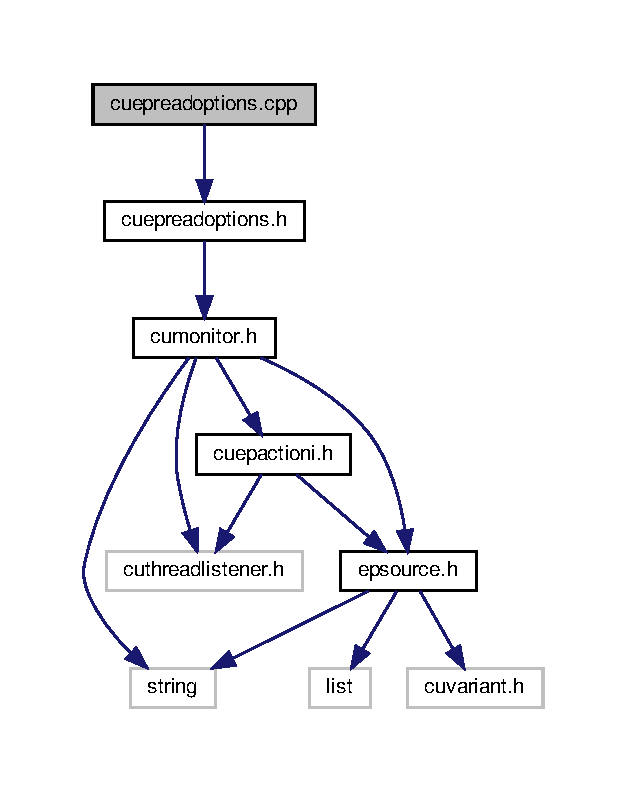
\includegraphics[width=301pt]{cuepreadoptions_8cpp__incl}
\end{center}
\end{figure}

\section{cuepreadoptions.\+h File Reference}
\label{cuepreadoptions_8h}\index{cuepreadoptions.\+h@{cuepreadoptions.\+h}}
{\ttfamily \#include $<$cumonitor.\+h$>$}\newline
Include dependency graph for cuepreadoptions.\+h\+:\nopagebreak
\begin{figure}[H]
\begin{center}
\leavevmode
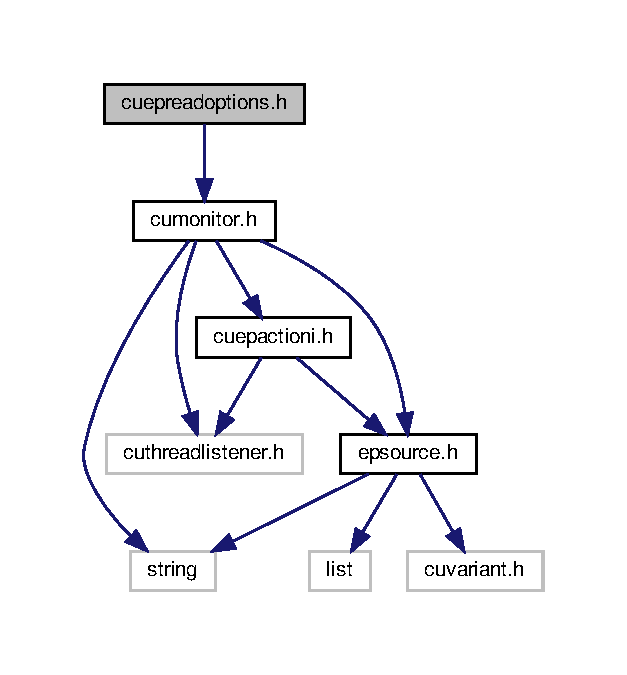
\includegraphics[width=301pt]{cuepreadoptions_8h__incl}
\end{center}
\end{figure}
This graph shows which files directly or indirectly include this file\+:\nopagebreak
\begin{figure}[H]
\begin{center}
\leavevmode
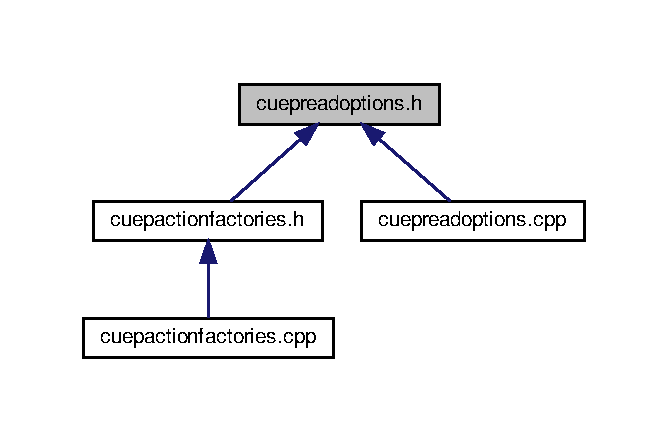
\includegraphics[width=321pt]{cuepreadoptions_8h__dep__incl}
\end{center}
\end{figure}
\subsection*{Classes}
\begin{DoxyCompactItemize}
\item 
class \textbf{ Cu\+Epics\+Read\+Options}
\end{DoxyCompactItemize}

\section{cumbiaepics.\+cpp File Reference}
\label{cumbiaepics_8cpp}\index{cumbiaepics.\+cpp@{cumbiaepics.\+cpp}}
{\ttfamily \#include \char`\"{}cumbiaepics.\+h\char`\"{}}\newline
{\ttfamily \#include $<$cumbia.\+h$>$}\newline
{\ttfamily \#include $<$culog.\+h$>$}\newline
{\ttfamily \#include $<$cumacros.\+h$>$}\newline
{\ttfamily \#include $<$cudatalistener.\+h$>$}\newline
{\ttfamily \#include $<$cuserviceprovider.\+h$>$}\newline
{\ttfamily \#include \char`\"{}cuepactionfactoryservice.\+h\char`\"{}}\newline
{\ttfamily \#include \char`\"{}cuepactionfactoryi.\+h\char`\"{}}\newline
{\ttfamily \#include \char`\"{}cuepcaservice.\+h\char`\"{}}\newline
{\ttfamily \#include \char`\"{}cuepics-\/world.\+h\char`\"{}}\newline
{\ttfamily \#include \char`\"{}cumonitor.\+h\char`\"{}}\newline
{\ttfamily \#include $<$cuthreadfactoryimpl.\+h$>$}\newline
{\ttfamily \#include $<$cuthreadseventbridgefactory\+\_\+i.\+h$>$}\newline
Include dependency graph for cumbiaepics.\+cpp\+:\nopagebreak
\begin{figure}[H]
\begin{center}
\leavevmode
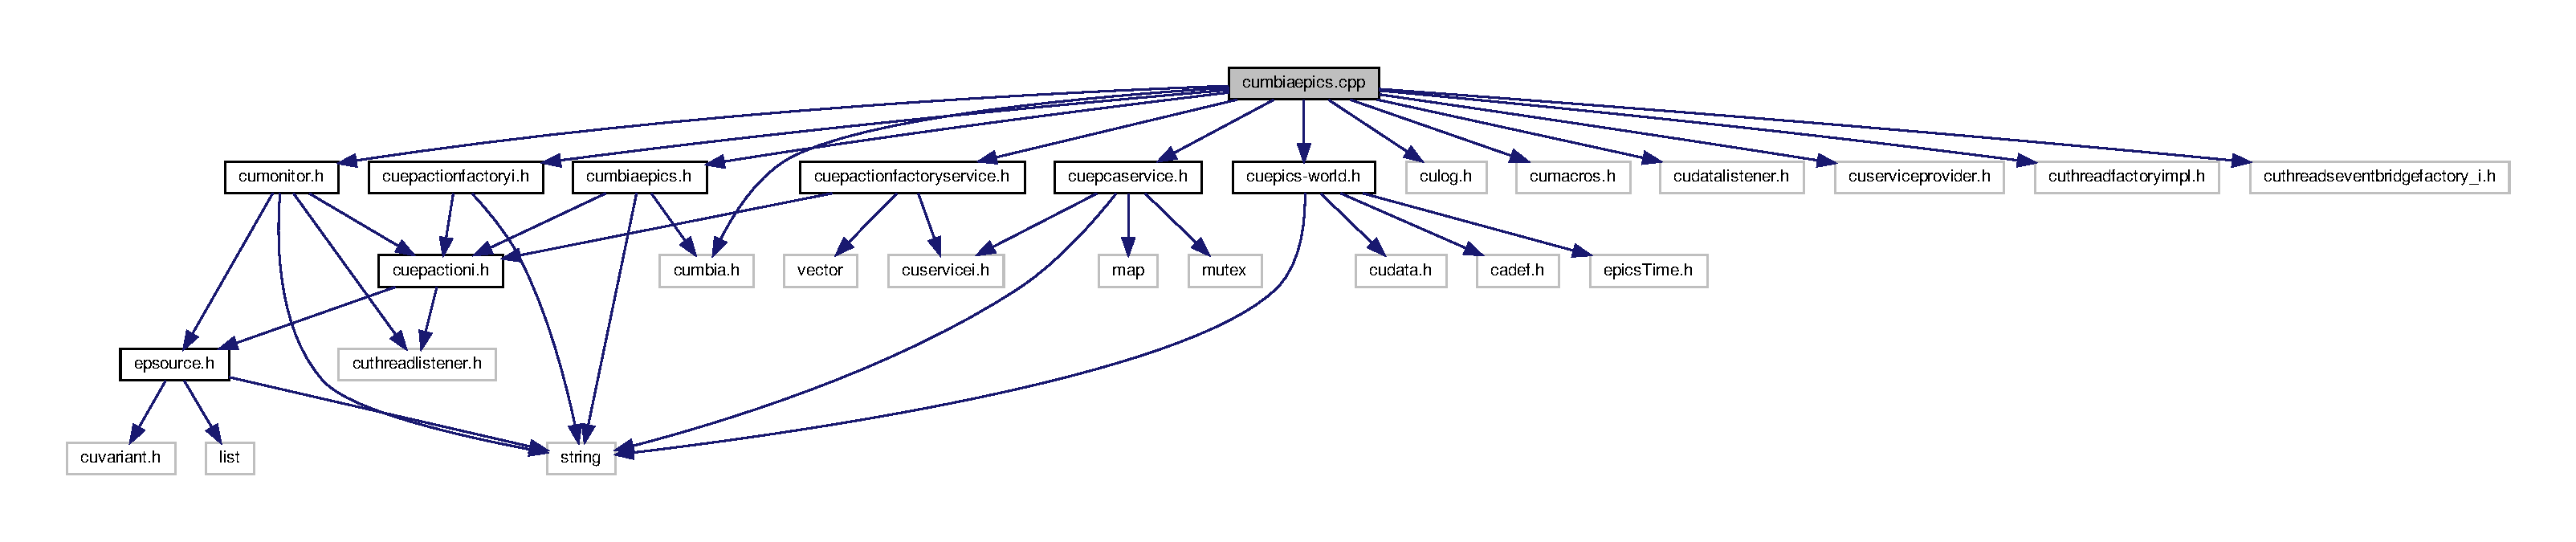
\includegraphics[width=350pt]{cumbiaepics_8cpp__incl}
\end{center}
\end{figure}

\section{cumbiaepics.\+h File Reference}
\label{cumbiaepics_8h}\index{cumbiaepics.\+h@{cumbiaepics.\+h}}
{\ttfamily \#include $<$cumbia.\+h$>$}\newline
{\ttfamily \#include \char`\"{}cuepactioni.\+h\char`\"{}}\newline
{\ttfamily \#include $<$string$>$}\newline
Include dependency graph for cumbiaepics.\+h\+:\nopagebreak
\begin{figure}[H]
\begin{center}
\leavevmode
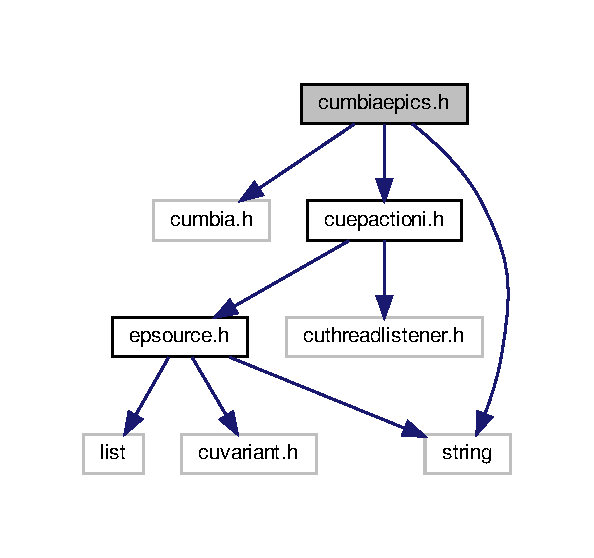
\includegraphics[width=285pt]{cumbiaepics_8h__incl}
\end{center}
\end{figure}
This graph shows which files directly or indirectly include this file\+:\nopagebreak
\begin{figure}[H]
\begin{center}
\leavevmode
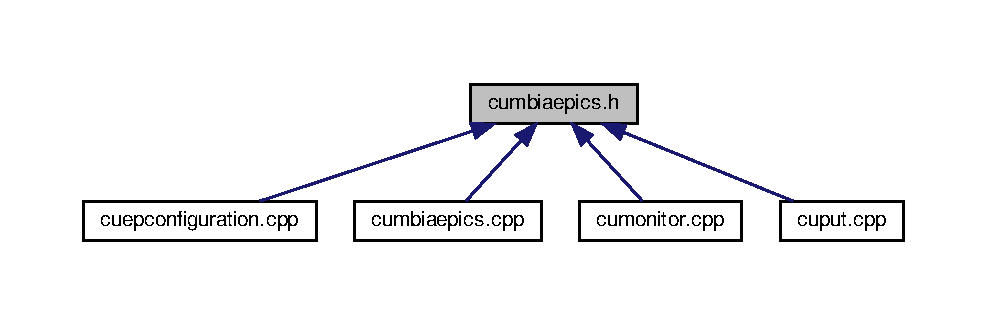
\includegraphics[width=350pt]{cumbiaepics_8h__dep__incl}
\end{center}
\end{figure}
\subsection*{Classes}
\begin{DoxyCompactItemize}
\item 
class \textbf{ Cumbia\+Epics}
\begin{DoxyCompactList}\small\item\em Cumbia implementation over the E\+P\+I\+CS control system. \end{DoxyCompactList}\end{DoxyCompactItemize}

\section{cumonitor.\+cpp File Reference}
\label{cumonitor_8cpp}\index{cumonitor.\+cpp@{cumonitor.\+cpp}}
{\ttfamily \#include \char`\"{}cumonitor.\+h\char`\"{}}\newline
{\ttfamily \#include \char`\"{}cumbiaepics.\+h\char`\"{}}\newline
{\ttfamily \#include \char`\"{}cuepactionfactoryservice.\+h\char`\"{}}\newline
{\ttfamily \#include \char`\"{}cuepcaservice.\+h\char`\"{}}\newline
{\ttfamily \#include \char`\"{}epsource.\+h\char`\"{}}\newline
{\ttfamily \#include $<$cudatalistener.\+h$>$}\newline
{\ttfamily \#include $<$cuserviceprovider.\+h$>$}\newline
{\ttfamily \#include $<$cumacros.\+h$>$}\newline
{\ttfamily \#include $<$list$>$}\newline
{\ttfamily \#include $<$cuthreadfactoryimpl\+\_\+i.\+h$>$}\newline
{\ttfamily \#include $<$cuthreadseventbridgefactory\+\_\+i.\+h$>$}\newline
{\ttfamily \#include $<$cuactivitymanager.\+h$>$}\newline
{\ttfamily \#include \char`\"{}cumonitoractivity.\+h\char`\"{}}\newline
{\ttfamily \#include $<$culog.\+h$>$}\newline
{\ttfamily \#include $<$cadef.\+h$>$}\newline
Include dependency graph for cumonitor.\+cpp\+:\nopagebreak
\begin{figure}[H]
\begin{center}
\leavevmode
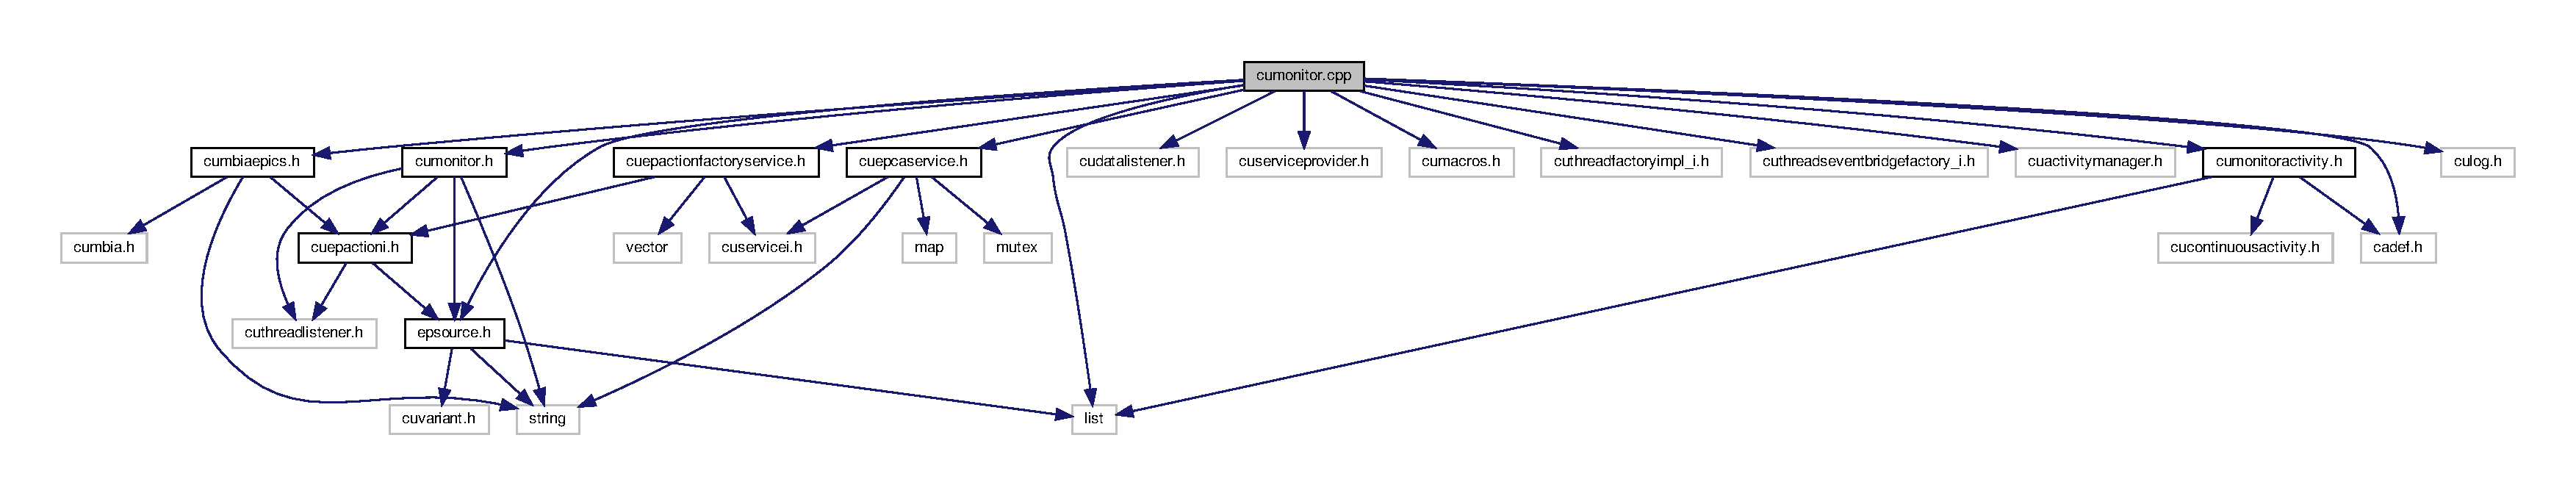
\includegraphics[width=350pt]{cumonitor_8cpp__incl}
\end{center}
\end{figure}
\subsection*{Classes}
\begin{DoxyCompactItemize}
\item 
class \textbf{ Cu\+Monitor\+Private}
\end{DoxyCompactItemize}

\section{cumonitor.\+h File Reference}
\label{cumonitor_8h}\index{cumonitor.\+h@{cumonitor.\+h}}
{\ttfamily \#include $<$string$>$}\newline
{\ttfamily \#include $<$cuthreadlistener.\+h$>$}\newline
{\ttfamily \#include $<$epsource.\+h$>$}\newline
{\ttfamily \#include $<$cuepactioni.\+h$>$}\newline
Include dependency graph for cumonitor.\+h\+:\nopagebreak
\begin{figure}[H]
\begin{center}
\leavevmode
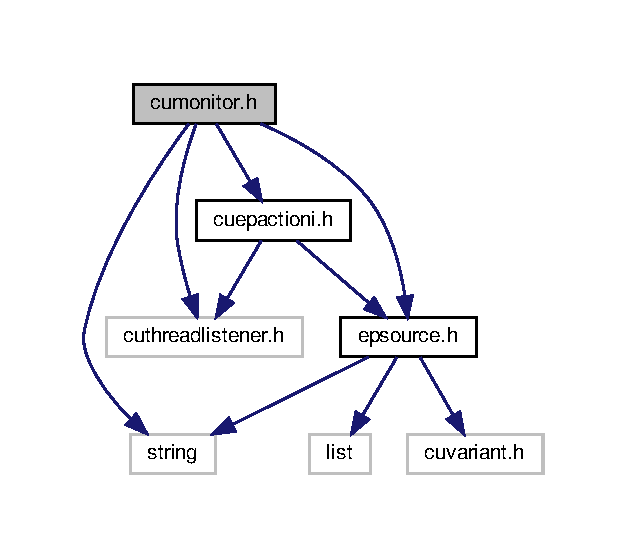
\includegraphics[width=301pt]{cumonitor_8h__incl}
\end{center}
\end{figure}
This graph shows which files directly or indirectly include this file\+:\nopagebreak
\begin{figure}[H]
\begin{center}
\leavevmode
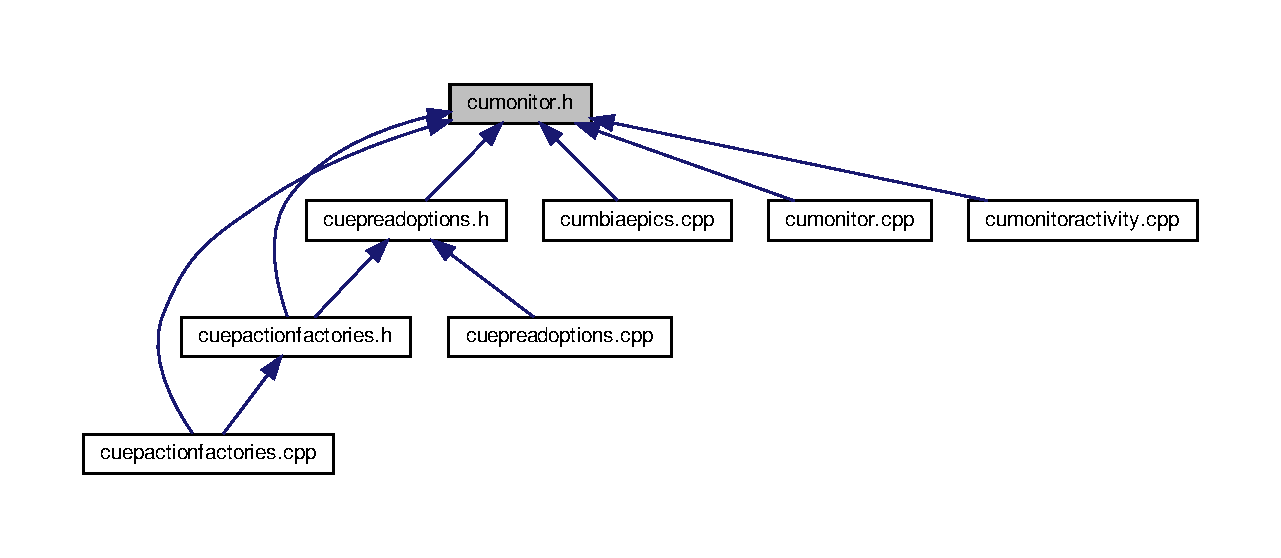
\includegraphics[width=350pt]{cumonitor_8h__dep__incl}
\end{center}
\end{figure}
\subsection*{Classes}
\begin{DoxyCompactItemize}
\item 
class \textbf{ Cu\+Monitor}
\end{DoxyCompactItemize}

\section{cumonitoractivity.\+cpp File Reference}
\label{cumonitoractivity_8cpp}\index{cumonitoractivity.\+cpp@{cumonitoractivity.\+cpp}}
{\ttfamily \#include \char`\"{}cumonitor.\+h\char`\"{}}\newline
{\ttfamily \#include \char`\"{}cumonitoractivity.\+h\char`\"{}}\newline
{\ttfamily \#include \char`\"{}epsource.\+h\char`\"{}}\newline
{\ttfamily \#include \char`\"{}cuepics-\/world.\+h\char`\"{}}\newline
{\ttfamily \#include $<$cadef.\+h$>$}\newline
{\ttfamily \#include $<$cumacros.\+h$>$}\newline
{\ttfamily \#include $<$stdlib.\+h$>$}\newline
{\ttfamily \#include $<$string.\+h$>$}\newline
{\ttfamily \#include $<$cuactivitymanager.\+h$>$}\newline
Include dependency graph for cumonitoractivity.\+cpp\+:\nopagebreak
\begin{figure}[H]
\begin{center}
\leavevmode
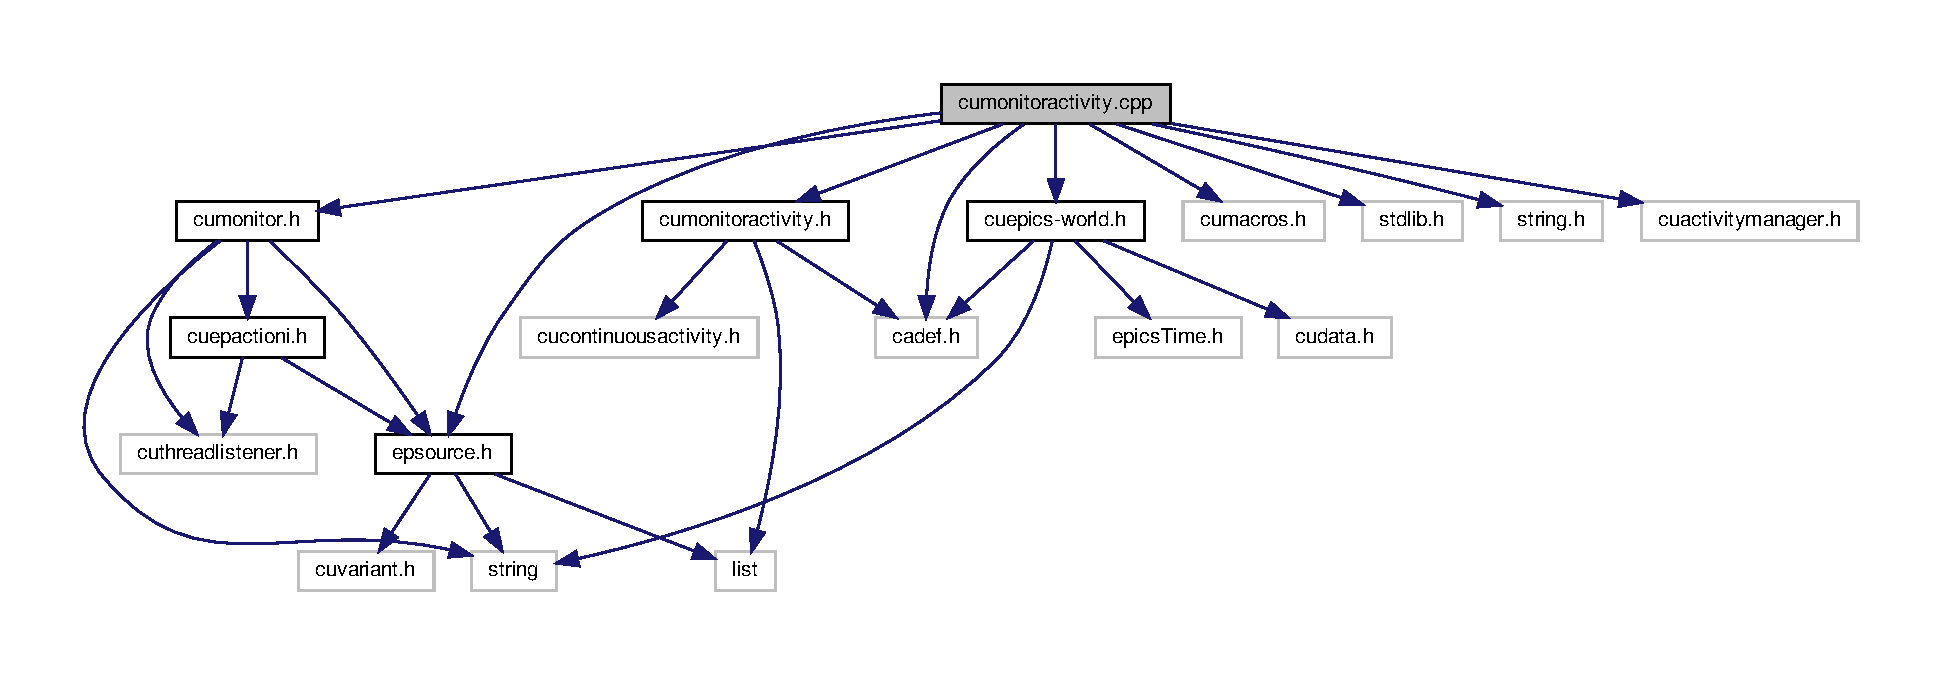
\includegraphics[width=350pt]{cumonitoractivity_8cpp__incl}
\end{center}
\end{figure}
\subsection*{Classes}
\begin{DoxyCompactItemize}
\item 
class \textbf{ Cu\+Monitor\+Activity\+Private}
\end{DoxyCompactItemize}

\section{cumonitoractivity.\+h File Reference}
\label{cumonitoractivity_8h}\index{cumonitoractivity.\+h@{cumonitoractivity.\+h}}
{\ttfamily \#include $<$cucontinuousactivity.\+h$>$}\newline
{\ttfamily \#include $<$list$>$}\newline
{\ttfamily \#include $<$cadef.\+h$>$}\newline
Include dependency graph for cumonitoractivity.\+h\+:\nopagebreak
\begin{figure}[H]
\begin{center}
\leavevmode
\includegraphics[width=309pt]{cumonitoractivity_8h__incl}
\end{center}
\end{figure}
This graph shows which files directly or indirectly include this file\+:\nopagebreak
\begin{figure}[H]
\begin{center}
\leavevmode
\includegraphics[width=286pt]{cumonitoractivity_8h__dep__incl}
\end{center}
\end{figure}
\subsection*{Classes}
\begin{DoxyCompactItemize}
\item 
class \textbf{ Cu\+Monitor\+Activity}
\end{DoxyCompactItemize}

\section{cuput.\+cpp File Reference}
\label{cuput_8cpp}\index{cuput.\+cpp@{cuput.\+cpp}}
{\ttfamily \#include \char`\"{}cuput.\+h\char`\"{}}\newline
{\ttfamily \#include \char`\"{}cumbiaepics.\+h\char`\"{}}\newline
{\ttfamily \#include \char`\"{}cuputactivity.\+h\char`\"{}}\newline
{\ttfamily \#include \char`\"{}cuepactionfactoryservice.\+h\char`\"{}}\newline
{\ttfamily \#include \char`\"{}cuepcaservice.\+h\char`\"{}}\newline
{\ttfamily \#include $<$cudatalistener.\+h$>$}\newline
{\ttfamily \#include $<$cuserviceprovider.\+h$>$}\newline
{\ttfamily \#include $<$cumacros.\+h$>$}\newline
{\ttfamily \#include $<$list$>$}\newline
{\ttfamily \#include $<$cuthreadfactoryimpl\+\_\+i.\+h$>$}\newline
{\ttfamily \#include $<$cuthreadseventbridgefactory\+\_\+i.\+h$>$}\newline
{\ttfamily \#include $<$cuactivitymanager.\+h$>$}\newline
{\ttfamily \#include $<$culog.\+h$>$}\newline
{\ttfamily \#include $<$cadef.\+h$>$}\newline
Include dependency graph for cuput.\+cpp\+:\nopagebreak
\begin{figure}[H]
\begin{center}
\leavevmode
\includegraphics[width=350pt]{cuput_8cpp__incl}
\end{center}
\end{figure}
\subsection*{Classes}
\begin{DoxyCompactItemize}
\item 
class \textbf{ Cu\+T\+Writer\+Private}
\end{DoxyCompactItemize}

\section{cuput.\+h File Reference}
\label{cuput_8h}\index{cuput.\+h@{cuput.\+h}}
{\ttfamily \#include $<$cuepactioni.\+h$>$}\newline
Include dependency graph for cuput.\+h\+:\nopagebreak
\begin{figure}[H]
\begin{center}
\leavevmode
\includegraphics[width=299pt]{cuput_8h__incl}
\end{center}
\end{figure}
This graph shows which files directly or indirectly include this file\+:\nopagebreak
\begin{figure}[H]
\begin{center}
\leavevmode
\includegraphics[width=278pt]{cuput_8h__dep__incl}
\end{center}
\end{figure}
\subsection*{Classes}
\begin{DoxyCompactItemize}
\item 
class \textbf{ Cu\+Put}
\end{DoxyCompactItemize}

\section{cuputactivity.\+cpp File Reference}
\label{cuputactivity_8cpp}\index{cuputactivity.\+cpp@{cuputactivity.\+cpp}}
{\ttfamily \#include \char`\"{}cuputactivity.\+h\char`\"{}}\newline
{\ttfamily \#include \char`\"{}cuepactioni.\+h\char`\"{}}\newline
{\ttfamily \#include \char`\"{}cuepics-\/world.\+h\char`\"{}}\newline
{\ttfamily \#include \char`\"{}cuepcaservice.\+h\char`\"{}}\newline
{\ttfamily \#include $<$cumacros.\+h$>$}\newline
Include dependency graph for cuputactivity.\+cpp\+:\nopagebreak
\begin{figure}[H]
\begin{center}
\leavevmode
\includegraphics[width=350pt]{cuputactivity_8cpp__incl}
\end{center}
\end{figure}
\subsection*{Classes}
\begin{DoxyCompactItemize}
\item 
class \textbf{ Cu\+Write\+Activity\+Private}
\end{DoxyCompactItemize}

\section{cuputactivity.\+h File Reference}
\label{cuputactivity_8h}\index{cuputactivity.\+h@{cuputactivity.\+h}}
{\ttfamily \#include $<$cuisolatedactivity.\+h$>$}\newline
Include dependency graph for cuputactivity.\+h\+:\nopagebreak
\begin{figure}[H]
\begin{center}
\leavevmode
\includegraphics[width=181pt]{cuputactivity_8h__incl}
\end{center}
\end{figure}
This graph shows which files directly or indirectly include this file\+:\nopagebreak
\begin{figure}[H]
\begin{center}
\leavevmode
\includegraphics[width=248pt]{cuputactivity_8h__dep__incl}
\end{center}
\end{figure}
\subsection*{Classes}
\begin{DoxyCompactItemize}
\item 
class \textbf{ Cu\+Write\+Activity}
\end{DoxyCompactItemize}

\section{epsource.\+cpp File Reference}
\label{epsource_8cpp}\index{epsource.\+cpp@{epsource.\+cpp}}
{\ttfamily \#include $<$stdio.\+h$>$}\newline
{\ttfamily \#include $<$algorithm$>$}\newline
{\ttfamily \#include $<$regex$>$}\newline
{\ttfamily \#include $<$cumacros.\+h$>$}\newline
{\ttfamily \#include \char`\"{}epsource.\+h\char`\"{}}\newline
Include dependency graph for epsource.\+cpp\+:\nopagebreak
\begin{figure}[H]
\begin{center}
\leavevmode
\includegraphics[width=350pt]{epsource_8cpp__incl}
\end{center}
\end{figure}

\section{epsource.\+h File Reference}
\label{epsource_8h}\index{epsource.\+h@{epsource.\+h}}
{\ttfamily \#include $<$string$>$}\newline
{\ttfamily \#include $<$list$>$}\newline
{\ttfamily \#include $<$cuvariant.\+h$>$}\newline
Include dependency graph for epsource.\+h\+:\nopagebreak
\begin{figure}[H]
\begin{center}
\leavevmode
\includegraphics[width=251pt]{epsource_8h__incl}
\end{center}
\end{figure}
This graph shows which files directly or indirectly include this file\+:\nopagebreak
\begin{figure}[H]
\begin{center}
\leavevmode
\includegraphics[width=350pt]{epsource_8h__dep__incl}
\end{center}
\end{figure}
\subsection*{Classes}
\begin{DoxyCompactItemize}
\item 
class \textbf{ Ep\+Source}
\end{DoxyCompactItemize}

%--- End generated contents ---

% Index
\backmatter
\newpage
\phantomsection
\clearemptydoublepage
\addcontentsline{toc}{chapter}{Index}
\printindex

\end{document}
